% Options for packages loaded elsewhere
\PassOptionsToPackage{unicode}{hyperref}
\PassOptionsToPackage{hyphens}{url}
\PassOptionsToPackage{dvipsnames,svgnames,x11names}{xcolor}
%
\documentclass[
  letterpaper,
  DIV=11,
  numbers=noendperiod]{scrreprt}

\usepackage{amsmath,amssymb}
\usepackage{lmodern}
\usepackage{iftex}
\ifPDFTeX
  \usepackage[T1]{fontenc}
  \usepackage[utf8]{inputenc}
  \usepackage{textcomp} % provide euro and other symbols
\else % if luatex or xetex
  \usepackage{unicode-math}
  \defaultfontfeatures{Scale=MatchLowercase}
  \defaultfontfeatures[\rmfamily]{Ligatures=TeX,Scale=1}
\fi
% Use upquote if available, for straight quotes in verbatim environments
\IfFileExists{upquote.sty}{\usepackage{upquote}}{}
\IfFileExists{microtype.sty}{% use microtype if available
  \usepackage[]{microtype}
  \UseMicrotypeSet[protrusion]{basicmath} % disable protrusion for tt fonts
}{}
\makeatletter
\@ifundefined{KOMAClassName}{% if non-KOMA class
  \IfFileExists{parskip.sty}{%
    \usepackage{parskip}
  }{% else
    \setlength{\parindent}{0pt}
    \setlength{\parskip}{6pt plus 2pt minus 1pt}}
}{% if KOMA class
  \KOMAoptions{parskip=half}}
\makeatother
\usepackage{xcolor}
\setlength{\emergencystretch}{3em} % prevent overfull lines
\setcounter{secnumdepth}{5}
% Make \paragraph and \subparagraph free-standing
\ifx\paragraph\undefined\else
  \let\oldparagraph\paragraph
  \renewcommand{\paragraph}[1]{\oldparagraph{#1}\mbox{}}
\fi
\ifx\subparagraph\undefined\else
  \let\oldsubparagraph\subparagraph
  \renewcommand{\subparagraph}[1]{\oldsubparagraph{#1}\mbox{}}
\fi

\usepackage{color}
\usepackage{fancyvrb}
\newcommand{\VerbBar}{|}
\newcommand{\VERB}{\Verb[commandchars=\\\{\}]}
\DefineVerbatimEnvironment{Highlighting}{Verbatim}{commandchars=\\\{\}}
% Add ',fontsize=\small' for more characters per line
\usepackage{framed}
\definecolor{shadecolor}{RGB}{241,243,245}
\newenvironment{Shaded}{\begin{snugshade}}{\end{snugshade}}
\newcommand{\AlertTok}[1]{\textcolor[rgb]{0.68,0.00,0.00}{#1}}
\newcommand{\AnnotationTok}[1]{\textcolor[rgb]{0.37,0.37,0.37}{#1}}
\newcommand{\AttributeTok}[1]{\textcolor[rgb]{0.40,0.45,0.13}{#1}}
\newcommand{\BaseNTok}[1]{\textcolor[rgb]{0.68,0.00,0.00}{#1}}
\newcommand{\BuiltInTok}[1]{\textcolor[rgb]{0.00,0.23,0.31}{#1}}
\newcommand{\CharTok}[1]{\textcolor[rgb]{0.13,0.47,0.30}{#1}}
\newcommand{\CommentTok}[1]{\textcolor[rgb]{0.37,0.37,0.37}{#1}}
\newcommand{\CommentVarTok}[1]{\textcolor[rgb]{0.37,0.37,0.37}{\textit{#1}}}
\newcommand{\ConstantTok}[1]{\textcolor[rgb]{0.56,0.35,0.01}{#1}}
\newcommand{\ControlFlowTok}[1]{\textcolor[rgb]{0.00,0.23,0.31}{#1}}
\newcommand{\DataTypeTok}[1]{\textcolor[rgb]{0.68,0.00,0.00}{#1}}
\newcommand{\DecValTok}[1]{\textcolor[rgb]{0.68,0.00,0.00}{#1}}
\newcommand{\DocumentationTok}[1]{\textcolor[rgb]{0.37,0.37,0.37}{\textit{#1}}}
\newcommand{\ErrorTok}[1]{\textcolor[rgb]{0.68,0.00,0.00}{#1}}
\newcommand{\ExtensionTok}[1]{\textcolor[rgb]{0.00,0.23,0.31}{#1}}
\newcommand{\FloatTok}[1]{\textcolor[rgb]{0.68,0.00,0.00}{#1}}
\newcommand{\FunctionTok}[1]{\textcolor[rgb]{0.28,0.35,0.67}{#1}}
\newcommand{\ImportTok}[1]{\textcolor[rgb]{0.00,0.46,0.62}{#1}}
\newcommand{\InformationTok}[1]{\textcolor[rgb]{0.37,0.37,0.37}{#1}}
\newcommand{\KeywordTok}[1]{\textcolor[rgb]{0.00,0.23,0.31}{#1}}
\newcommand{\NormalTok}[1]{\textcolor[rgb]{0.00,0.23,0.31}{#1}}
\newcommand{\OperatorTok}[1]{\textcolor[rgb]{0.37,0.37,0.37}{#1}}
\newcommand{\OtherTok}[1]{\textcolor[rgb]{0.00,0.23,0.31}{#1}}
\newcommand{\PreprocessorTok}[1]{\textcolor[rgb]{0.68,0.00,0.00}{#1}}
\newcommand{\RegionMarkerTok}[1]{\textcolor[rgb]{0.00,0.23,0.31}{#1}}
\newcommand{\SpecialCharTok}[1]{\textcolor[rgb]{0.37,0.37,0.37}{#1}}
\newcommand{\SpecialStringTok}[1]{\textcolor[rgb]{0.13,0.47,0.30}{#1}}
\newcommand{\StringTok}[1]{\textcolor[rgb]{0.13,0.47,0.30}{#1}}
\newcommand{\VariableTok}[1]{\textcolor[rgb]{0.07,0.07,0.07}{#1}}
\newcommand{\VerbatimStringTok}[1]{\textcolor[rgb]{0.13,0.47,0.30}{#1}}
\newcommand{\WarningTok}[1]{\textcolor[rgb]{0.37,0.37,0.37}{\textit{#1}}}

\providecommand{\tightlist}{%
  \setlength{\itemsep}{0pt}\setlength{\parskip}{0pt}}\usepackage{longtable,booktabs,array}
\usepackage{calc} % for calculating minipage widths
% Correct order of tables after \paragraph or \subparagraph
\usepackage{etoolbox}
\makeatletter
\patchcmd\longtable{\par}{\if@noskipsec\mbox{}\fi\par}{}{}
\makeatother
% Allow footnotes in longtable head/foot
\IfFileExists{footnotehyper.sty}{\usepackage{footnotehyper}}{\usepackage{footnote}}
\makesavenoteenv{longtable}
\usepackage{graphicx}
\makeatletter
\def\maxwidth{\ifdim\Gin@nat@width>\linewidth\linewidth\else\Gin@nat@width\fi}
\def\maxheight{\ifdim\Gin@nat@height>\textheight\textheight\else\Gin@nat@height\fi}
\makeatother
% Scale images if necessary, so that they will not overflow the page
% margins by default, and it is still possible to overwrite the defaults
% using explicit options in \includegraphics[width, height, ...]{}
\setkeys{Gin}{width=\maxwidth,height=\maxheight,keepaspectratio}
% Set default figure placement to htbp
\makeatletter
\def\fps@figure{htbp}
\makeatother
\newlength{\cslhangindent}
\setlength{\cslhangindent}{1.5em}
\newlength{\csllabelwidth}
\setlength{\csllabelwidth}{3em}
\newlength{\cslentryspacingunit} % times entry-spacing
\setlength{\cslentryspacingunit}{\parskip}
\newenvironment{CSLReferences}[2] % #1 hanging-ident, #2 entry spacing
 {% don't indent paragraphs
  \setlength{\parindent}{0pt}
  % turn on hanging indent if param 1 is 1
  \ifodd #1
  \let\oldpar\par
  \def\par{\hangindent=\cslhangindent\oldpar}
  \fi
  % set entry spacing
  \setlength{\parskip}{#2\cslentryspacingunit}
 }%
 {}
\usepackage{calc}
\newcommand{\CSLBlock}[1]{#1\hfill\break}
\newcommand{\CSLLeftMargin}[1]{\parbox[t]{\csllabelwidth}{#1}}
\newcommand{\CSLRightInline}[1]{\parbox[t]{\linewidth - \csllabelwidth}{#1}\break}
\newcommand{\CSLIndent}[1]{\hspace{\cslhangindent}#1}

\KOMAoption{captions}{tableheading}
\makeatletter
\@ifpackageloaded{tcolorbox}{}{\usepackage[many]{tcolorbox}}
\@ifpackageloaded{fontawesome5}{}{\usepackage{fontawesome5}}
\definecolor{quarto-callout-color}{HTML}{909090}
\definecolor{quarto-callout-note-color}{HTML}{0758E5}
\definecolor{quarto-callout-important-color}{HTML}{CC1914}
\definecolor{quarto-callout-warning-color}{HTML}{EB9113}
\definecolor{quarto-callout-tip-color}{HTML}{00A047}
\definecolor{quarto-callout-caution-color}{HTML}{FC5300}
\definecolor{quarto-callout-color-frame}{HTML}{acacac}
\definecolor{quarto-callout-note-color-frame}{HTML}{4582ec}
\definecolor{quarto-callout-important-color-frame}{HTML}{d9534f}
\definecolor{quarto-callout-warning-color-frame}{HTML}{f0ad4e}
\definecolor{quarto-callout-tip-color-frame}{HTML}{02b875}
\definecolor{quarto-callout-caution-color-frame}{HTML}{fd7e14}
\makeatother
\makeatletter
\makeatother
\makeatletter
\@ifpackageloaded{bookmark}{}{\usepackage{bookmark}}
\makeatother
\makeatletter
\@ifpackageloaded{caption}{}{\usepackage{caption}}
\AtBeginDocument{%
\ifdefined\contentsname
  \renewcommand*\contentsname{Table des matières}
\else
  \newcommand\contentsname{Table des matières}
\fi
\ifdefined\listfigurename
  \renewcommand*\listfigurename{Liste des Figures}
\else
  \newcommand\listfigurename{Liste des Figures}
\fi
\ifdefined\listtablename
  \renewcommand*\listtablename{Liste des Tables}
\else
  \newcommand\listtablename{Liste des Tables}
\fi
\ifdefined\figurename
  \renewcommand*\figurename{Figure}
\else
  \newcommand\figurename{Figure}
\fi
\ifdefined\tablename
  \renewcommand*\tablename{Table}
\else
  \newcommand\tablename{Table}
\fi
}
\@ifpackageloaded{float}{}{\usepackage{float}}
\floatstyle{ruled}
\@ifundefined{c@chapter}{\newfloat{codelisting}{h}{lop}}{\newfloat{codelisting}{h}{lop}[chapter]}
\floatname{codelisting}{Listing}
\newcommand*\listoflistings{\listof{codelisting}{Liste des Listings}}
\makeatother
\makeatletter
\@ifpackageloaded{caption}{}{\usepackage{caption}}
\@ifpackageloaded{subcaption}{}{\usepackage{subcaption}}
\makeatother
\makeatletter
\@ifpackageloaded{tcolorbox}{}{\usepackage[many]{tcolorbox}}
\makeatother
\makeatletter
\@ifundefined{shadecolor}{\definecolor{shadecolor}{rgb}{.97, .97, .97}}
\makeatother
\makeatletter
\makeatother
\makeatletter
\@ifpackageloaded{fontawesome5}{}{\usepackage{fontawesome5}}
\makeatother
\ifLuaTeX
\usepackage[bidi=basic]{babel}
\else
\usepackage[bidi=default]{babel}
\fi
\babelprovide[main,import]{french}
% get rid of language-specific shorthands (see #6817):
\let\LanguageShortHands\languageshorthands
\def\languageshorthands#1{}
\ifLuaTeX
  \usepackage{selnolig}  % disable illegal ligatures
\fi
\IfFileExists{bookmark.sty}{\usepackage{bookmark}}{\usepackage{hyperref}}
\IfFileExists{xurl.sty}{\usepackage{xurl}}{} % add URL line breaks if available
\urlstyle{same} % disable monospaced font for URLs
\hypersetup{
  pdftitle={TP de Biométrie  Semestre 3 },
  pdfauthor={Benoît Simon-Bouhet},
  pdflang={fr},
  colorlinks=true,
  linkcolor={blue},
  filecolor={Maroon},
  citecolor={Blue},
  urlcolor={Blue},
  pdfcreator={LaTeX via pandoc}}

\title{TP de Biométrie Semestre 3}
\author{Benoît Simon-Bouhet}
\date{2022-09-16T00:00:00+02:00}

\begin{document}
\maketitle
\ifdefined\Shaded\renewenvironment{Shaded}{\begin{tcolorbox}[borderline west={3pt}{0pt}{shadecolor}, enhanced, breakable, frame hidden, boxrule=0pt, sharp corners, interior hidden]}{\end{tcolorbox}}\fi

\renewcommand*\contentsname{Table des matières}
{
\hypersetup{linkcolor=}
\setcounter{tocdepth}{2}
\tableofcontents
}
\bookmarksetup{startatroot}

\hypertarget{introduction}{%
\chapter*{Introduction}\label{introduction}}
\addcontentsline{toc}{chapter}{Introduction}

\hypertarget{objectifs}{%
\section*{Objectifs}\label{objectifs}}
\addcontentsline{toc}{section}{Objectifs}

Ce livre contient l'ensemble du matériel (contenus, exemples,
exercices\ldots) nécessaire à la réalisation des travaux pratiques de
\textbf{Biométrie} de l'EC `\emph{Outils pour l'étude et la
compréhension du vivant 2}' du semestre 3 de la licence Sciences de la
Vie de La Rochelle Université.

Les 4 grands chapitres de ce livre correspondent aux 3 objectifs
principaux de ces séances de TP et TEA :

\begin{enumerate}
\def\labelenumi{\arabic{enumi}.}
\item
  \textbf{Vous faire découvrir les logiciels
  \href{https://cran.r-project.org}{R} et
  \href{https://www.rstudio.com}{Rstudio}} (chap.~1 et 2) dans lesquels
  vous allez passer beaucoup de temps en licence puis en master. Si vous
  choisissez une spécialité de master qui implique de traiter des
  données (c'est-à-dire à peu près toutes les spécialités des Sciences
  de la Vie !) et/ou de communiquer des résultats d'analyses
  statistiques, alors \texttt{R} et \texttt{RStudio} devraient être les
  logiciels vers lesquels vous vous tournerez naturellement.
\item
  \textbf{Vous apprendre à faire des graphiques de qualités} dans
  \texttt{RStudio} et \textbf{vous faire prendre conscience de
  l'importance des visualisations graphiques} (chap.~3) :
\end{enumerate}

\begin{itemize}
\tightlist
\item
  d'une part, pour explorer des données inconnues et vous faire une
  première idée des informations qu'elles contiennent,
\item
  d'autre part, pour vous permettre de formuler des hypothèses
  pertinentes et intéressantes concernant les systèmes que vous étudiez,
\item
  et enfin, pour communiquer efficacement vos trouvailles à un public
  qui ne connaît pas vos données aussi bien que vous (cela inclut
  évidemment vos enseignants à l'issue de vos stages).
\end{itemize}

\begin{enumerate}
\def\labelenumi{\arabic{enumi}.}
\setcounter{enumi}{2}
\tightlist
\item
  \textbf{Vous apprendre à manipuler efficacement des tableaux de
  données de grande taille} (chap.~4). Cela signifie que vous devriez
  être mesure de sélectionner des variables (colonnes) d'un tableau,
  d'en créer de nouvelles en modifiant et/ou combinant des variables
  existantes, de filtrer des lignes spécifiques, etc.
\end{enumerate}

À l'issue de ces TP et TEA, vous devriez donc être suffisamment à l'aise
avec le logiciel \texttt{RStudio} pour y importer des données issues de
tableurs, les manipuler pour les mettre dans un format permettant les
représentations graphiques, et pour produire des graphiques pertinents,
adaptés aux données dont vous disposez, et d'une qualité vous permettant
de les intégrer sans honte à vos compte-rendus de TP et rapports de
stages.

D'ailleurs, les données que vous serez amenés à traiter lors de vos
stages, ou plus tard, lorsque vous serez en poste, ont souvent été
acquises à grands frais, et au prix d'efforts importants. Il est donc de
votre responsabilité d'en tirer le maximum. Et ça commence toujours (ou
presque), par la manipulation de données dans \texttt{RStudio} et
réalisation de visualisations graphiques parlantes.

Dernière choses : à partir de maintenant, tous les compte-rendus de TP
que vous aurez à produire dans le cadre de la licence SV devront
respecter les bonnes pratiques décrites dans ce document. En
particulier, les collègues de l'équipe pédagogique attendent en effet
que les graphiques que vous intégrerez à vos compte-rendus de TP soient
systématiquement produits dans \texttt{RStudio}.

\begin{center}\rule{0.5\linewidth}{0.5pt}\end{center}

\hypertarget{organisation}{%
\section*{Organisation}\label{organisation}}
\addcontentsline{toc}{section}{Organisation}

\hypertarget{volume-de-travail}{%
\subsection*{Volume de travail}\label{volume-de-travail}}
\addcontentsline{toc}{subsection}{Volume de travail}

Les travaux pratiques et TEA de biométrie auront lieu entre le 12
septembre et le 07 octobre 2022 :

\begin{itemize}
\tightlist
\item
  Semaine 37 (du 12 au 16 septembre) : 1 séance de TP d'1h30 et 1 séance
  de TEA d'1h30
\item
  Semaine 38 (du 19 au 23 septembre) : 1 séance de TP d'1h30 et 1 séance
  de TEA d'1h30
\item
  Semaine 39 (du 26 au 30 septembre) : 1 séance de TP d'1h30
\item
  Semaine 40 (du 03 au 07 octobre) : 1 séance de TP d'1h30
\end{itemize}

\textbf{Tous les TP ont lieu en salle MSI 217. Tous les TEA sont à
distance.}

Au total, chaque groupe aura donc 4 séances de TP et 2 séances de TEA.
C'est très peu pour atteindre les objectifs fixés et il y aura donc
évidemment du travail personnel à fournir en dehors de ces séances. Pour
chaque TP ou TEA prévu à l'emploi du temps, j'estime qu'une à deux
heures de travail personnel est nécessaire (soit 9 à 15 heures au total,
selon votre degré d'aisance, à répartir sur 4 semaines). Attention donc
: pensez bien à prévoir du temps dans vos plannings car le travail
personnel est essentiel pour progresser dans cette matière. J'insiste
sur l'importance de faire l'effort dès maintenant : vous allez en effet
avoir des enseignements qui reposent sur l'utilisation de ces logiciels
à chaque semestre de la licence du S3 au S6. C'est maintenant qu'il faut
acquérir des automatismes, cela vous fera gagner énormément de temps
ensuite.

\hypertarget{modalituxe9s-denseignement}{%
\subsection*{Modalités
d'enseignement}\label{modalituxe9s-denseignement}}
\addcontentsline{toc}{subsection}{Modalités d'enseignement}

Pour suivre cet enseignement vous pourrez utiliser les ordinateurs de
l'université, mais je ne peux que vous encourager à utiliser vos propres
ordinateurs, sous Windows, Linux ou MacOS. Lors de vos futurs stages et
pour rédiger vos comptes-rendus de TP, vous utiliserez le plus souvent
vos propres ordinateurs, autant prendre dès maintenant de bonnes
habitudes en installant les logiciels dont vous aurez besoin tout au
long de votre licence. Si vous ne possédez pas d'ordinateur, manifestez
vous rapidement auprès de moi car des solutions existent (prêt par
l'université, travail sur tablette via
\href{https://rstudio.cloud}{RStudio cloud}\ldots).

\begin{tcolorbox}[enhanced jigsaw, bottomtitle=1mm, title=\textcolor{quarto-callout-important-color}{\faExclamation}\hspace{0.5em}{Important}, breakable, opacitybacktitle=0.6, coltitle=black, opacityback=0, toprule=.15mm, toptitle=1mm, titlerule=0mm, colback=white, rightrule=.15mm, arc=.35mm, leftrule=.75mm, bottomrule=.15mm, left=2mm, colframe=quarto-callout-important-color-frame, colbacktitle=quarto-callout-important-color!10!white]
L'essentiel du contenu de cet enseignement peut être abordé en
autonomie, à distance, grâce à ce livre en ligne, aux ressources mises à
disposition sur Moodle et à votre ordinateur personnel. Cela signifie
que \textbf{la présence physique lors de ces séances de TP n'est pas
obligatoire}.
\end{tcolorbox}

Plus que des séances de TP classiques, considérez plutôt qu'il s'agit de
\textbf{permanences non-obligatoires} : si vous pensez avoir besoin
d'aide, si vous avez des points de blocage ou des questions sur le
contenu de ce document, sur les exercices demandés ou sur les quizz
Moodle, alors venez poser vos questions lors des séances de TP. Vous ne
serez d'ailleurs pas tenus de rester pendant 1h30 : si vous obtenez une
réponse en 10 minutes et que vous préférez travailler ailleurs, vous
serez libres de repartir !

De même, si vous n'avez pas de difficulté de compréhension, que vous
n'avez pas de problème avec les exercices de ce livre en ligne ni avec
les quizz Moodle, votre présence n'est pas requise. Si vous souhaitez
malgré tout venir en salle de TP, pas de problème, vous y serez toujours
les bienvenus.

Ce fonctionnement très souple a de nombreux avantages :

\begin{itemize}
\tightlist
\item
  vous vous organisez comme vous le souhaitez
\item
  vous ne venez que lorsque vous en avez vraiment besoin
\item
  celles et ceux qui se déplacent reçoivent une aide personnalisée
\item
  vous travaillez sur vos ordinateurs
\item
  les effectifs étant réduits, c'est aussi plus confortable pour moi !
\end{itemize}

Toutefois, pour que cette organisation fonctionne, cela demande de la
rigueur de votre part, en particulier sur la régularité du travail que
vous devez fournir. Si la présence en salle de TP n'est pas requise, le
travail demandé est bel et bien obligatoire ! Si vous venez en salle de
TP sans avoir travaillé en amont, votre venue sera totalement inutile
puisque vous n'aurez pas de question à poser et que vous passerez votre
séance à lire ce livre en ligne. Vous perdrez donc votre temps, celui de
vos collègues, et le mien. De même, si vous attendez la 4e semaine pour
vous y mettre, vous irez droit dans le mur. Je le répète, outre les 9h
de TP/TEA prévus dans vos emplois du temps, vous devez prévoir entre 9
et 15 heures de travail personnel supplémentaire.

Je vous laisse donc une grande liberté d'organisation. À vous d'en tirer
le maximum et de faire preuve du sérieux nécessaire. Le rythme auquel
vous devriez avancer est présenté dans la partie suivante intitulée
``Progression conseillée''.

\hypertarget{utilisation-de-slack}{%
\subsection*{Utilisation de Slack}\label{utilisation-de-slack}}
\addcontentsline{toc}{subsection}{Utilisation de Slack}

Outre les séances de permanence non-obligatoires, nous échangerons aussi
sur \href{https://slack.com/intl/fr-fr/}{l'application Slack}, qui
fonctionne un peu comme un ``twitter privé''. Slack facilite la
communication des équipes et permet de travailler ensemble. Créez-vous
un compte en ligne et installez le logiciel sur votre ordinateur (il
existe aussi des versions pour tablettes et smartphones). Lorsque vous
aurez installé le logiciel,
\href{https://join.slack.com/t/l2sv22-23ecoutils/shared_invite/zt-1g7vrl3v7-k_B2D2kMmuRdv_T237Oluw}{cliquez
sur ce lien} pour vous connecter à notre espace de travail commun
intitulé \texttt{L2\ SV\ 22-23\ /\ EC\ outils} (ce lien expire
régulièrement : faites moi signe s'il n'est plus valide).

Vous verrez que 2 ``chaînes'' sont disponibles :

\begin{itemize}
\tightlist
\item
  \#général : c'est là que les questions liées à l'organisation générale
  du cours, des TP et TEA doivent être posées. Si vous ne savez pas si
  une séance de permanence a lieu, posez la question ici.
\item
  \#questions-rstudio : c'est ici que toutes les questions pratiques
  liées à l'utilisation de \texttt{R} et \texttt{RStudio} devront êtres
  posées. Problèmes de syntaxe, problèmes liés à l'interface, à
  l'installation des packages ou à l'utilisation des fonctions, à la
  création des graphiques, à la manipulation des tableaux\ldots{} Tout
  ce qui concerne directement les logiciels sera traité ici. Vous êtes
  libres de poser des questions, de poster des captures d'écran, des
  morceaux de code, des messages d'erreur. Et \textbf{vous êtes bien
  entendus vivement encouragés à vous entraider et à répondre aux
  questions de vos collègues.} Je n'interviendrai ici que pour répondre
  aux questions laissées sans réponse ou si les réponses apportées sont
  inexactes. Le fonctionnement est celui d'un forum de discussion
  instantané. Vous en tirerez le plus grand bénéfice en participant et
  en n'ayant pas peur de poser des questions, même si elles vous
  paraissent idiotes. Rappelez-vous toujours que si vous vous posez une
  question, d'autres se la posent aussi probablement.
\end{itemize}

Ainsi, quand vous travaillerez à vos TP ou TEA, que vous soyez installés
chez vous ou en salle de TP, prenez l'habitude de garder Slack ouvert
sur votre ordinateur. Même si vous n'avez pas de question à poser, votre
participation active pour répondre à vos collègues est souhaitable et
souhaitée. Je vous incite donc fortement à vous \textbf{entraider} :
c'est très formateur pour celui qui explique, et celui qui rencontre une
difficulté a plus de chances de comprendre si c'est quelqu'un d'autre
qui lui explique plutôt que la personne qui a rédigé les instructions
mal comprises.

Ce document est fait pour vous permettre d'avancer en autonomie et vous
ne devriez normalement pas avoir beaucoup besoin de moi si votre lecture
est attentive. L'expérience montre en effet que la plupart du temps, il
suffit de lire correctement les paragraphes précédents et/ou suivants
pour obtenir la réponse à ses questions. J'essaie néanmoins de rester
disponible sur Slack pendant les séances de TP et de TEA de tous les
groupes. Cela veut donc dire que même si votre groupe n'est pas en TP,
vos questions ont des chances d'être lues et de recevoir des réponses
dès que d'autres groupes sont en TP ou TEA. Vous êtes d'ailleurs
encouragés à échanger sur Slack aussi pendant vos phases de travail
personnels.

\hypertarget{progession-conseilluxe9e}{%
\section*{Progession conseillée}\label{progession-conseilluxe9e}}
\addcontentsline{toc}{section}{Progession conseillée}

Pour apprendre à utiliser un logiciel comme \texttt{R}, il faut faire
les choses soi-même, ne pas avoir peur des messages d'erreurs (il faut
d'ailleurs apprendre à les déchiffrer pour comprendre d'où viennent les
problèmes), essayer maintes fois, se tromper beaucoup, recommencer, et
surtout, ne pas se décourager. J'utilise ce logiciel presque
quotidiennement depuis plus de 15 ans et à chaque session de travail, je
rencontre des messages d'erreur. Avec suffisamment d'habitude, on
apprend à les déchiffrer, et on corrige les problèmes en quelques
secondes. Ce livre est conçu pour vous faciliter la tâche, mais ne vous
y trompez pas, vous rencontrerez des difficultés, et c'est normal. C'est
le prix à payer pour profiter de la puissance du meilleur logiciel
permettant d'analyser des données, de produire des graphiques de qualité
et de réaliser toutes les statistiques dont vous aurez besoin d'ici la
fin de vos études et au-delà.

Pour que cet apprentissage soit le moins problématique possible, il
convient de prendre les choses dans l'ordre. C'est la raison pour
laquelle les chapitres de ce livre doivent être lus dans l'ordre, et les
exercices d'application faits au fur et à mesure de la lecture.

Idéalement, voilà les étapes que vous devriez avoir franchi chaque
semaine :

\begin{enumerate}
\def\labelenumi{\arabic{enumi}.}
\item
  La première semaine (37) est consacrée à l'installation des logiciels,
  à la découverte de l'environnement de travail, des \texttt{RProjects},
  des packages et des scripts. Avant votre deuxième séance, vous devrez
  être capables de créer un Rproject et un script, de télécharger et
  d'installer des packages, et d'exécuter des commandes simples dans
  votre script. Vous devrez avoir suivi les tutoriels de DataCamp et
  connaitre les types d'objets suivants : vecteurs, facteurs,
  data.frames (et tibbles). Vous devrez effectuer le premier quizz
  Moodle (attention, ce quizz est à faire seul !).
\item
  La deuxième semaine (38) est consacrée à la découverte des premiers
  jeux de données et du package \texttt{ggplot2}. Avant votre troisième
  séance, vous devrez avoir compris comment charger en mémoire les jeux
  de données disponibles dans un packages, vous devrez connaitre la
  syntaxe de base permettant de faire toutes sortes de graphiques avec
  \texttt{ggplot2} avec une ou deux variables. À terme, vous devrez être
  capables de choisir des graphiques appropriés selon le nombre et la
  nature des variables dont vous disposez. À ce stade, on ne demande
  rien de complexe, mais vous devrez, à minima, être capable de faire
  des barplots, des histogrammes et des nuages de points. Vous devrez
  effectuer le second quizz Moodle (attention, ce quizz est à faire seul
  !).
\item
  La troisième semaine (39) est consacrée à l'amélioration de la qualité
  de vos graphiques. Avant votre dernière séance de TP, vous devrez être
  capable de faire, outre les graphiques de la semaine précédente, des
  stripcharts, et des graphiques en lignes et des boxplots. Vous devrez
  également être capable de faire des sous-graphiques par catégories
  (\texttt{facet()}), de choisir un thème et des palettes de couleurs
  appropriées, et de légender/annoter correctement vos graphiques. Vous
  devrez effectuer le troisième quizz Moodle (attention, ce quizz est à
  faire seul !).
\item
  La quatrième semaine (40) est consacrée à la manipulation des tableaux
  de données. Avant la fin de cette semaine, vous devrez être capable de
  sélectionner des colonnes dans un tableau, de filtrer des lignes, et
  de créer de nouvelles variables. Vous devrez être capables d'enchaîner
  correctement les étapes suivantes : ouvrir le logiciel \textgreater{}
  créer un projet \textgreater{} créer un script \textgreater{} mettre
  en mémoire les packages utiles \textgreater{} importer des données
  \textgreater{} mettre en forme ces données \textgreater{} faire un ou
  des graphiques informatifs et correctement mis en forme. Vous devrez
  effectuer le quatrième et dernier quizz Moodle (attention, ce quizz
  est à faire seul !).
\end{enumerate}

\hypertarget{uxe9valuations}{%
\section*{Évaluation(s)}\label{uxe9valuations}}
\addcontentsline{toc}{section}{Évaluation(s)}

Vous serez évalués à 3 niveaux :

\begin{enumerate}
\def\labelenumi{\arabic{enumi}.}
\tightlist
\item
  Votre participation sur Slack
\item
  Les quizz Moodle
\item
  Une évaluation plus classique
\end{enumerate}

Les exercices demandés dans ce document en ligne ne seront ni ramassés,
ni notés : ils sont proposés pour que vous puissiez mettre en
application les notions récemment apprises et afin d'évaluer votre
propre progression et vos apprentissages. Mais tout ce que nous voyons
en TP et TEA devra être acquis à la fin des TP.

En particulier, je vérifierai que les étapes décrites précédemment sont
maîtrisées (ouvrir le logiciel \textgreater{} créer un projet
\textgreater{} créer un script \textgreater{} mettre en mémoire les
packages utiles \textgreater{} importer des données \textgreater{}
mettre en forme ces données \textgreater{} faire un ou des graphiques
informatifs et correctement mis en forme) en vous fournissant un jeu de
données inconnu que vous devrez importer et mettre en forme dans
\texttt{RStudio} afin de produire quelques graphiques informatifs. Cette
évaluation aura lieu soit en salle informatique, soit dans le cadre d'un
compte-rendu de TP que vous devrez rendre pour un collègue. Si cette
modalité est mise en place, je vous en dirai plus en temps utile.

\bookmarksetup{startatroot}

\hypertarget{sec-bases}{%
\chapter{R et RStudio : les bases}\label{sec-bases}}

\hypertarget{pruxe9ambule}{%
\section{Préambule}\label{pruxe9ambule}}

Avant de commencer à explorer des données dans \texttt{R}, il y a
plusieurs concepts clés qu'il faut comprendre en premier lieu :

\begin{enumerate}
\def\labelenumi{\arabic{enumi}.}
\tightlist
\item
  Que sont \texttt{R} et \texttt{RStudio} ?
\item
  Comment s'y prend-on pour coder dans \texttt{R} ?
\item
  Que sont les \texttt{packages} ?
\end{enumerate}

Une bonne maîtrise des éléments présentés dans ce chapitre est
indispensable pour aborder sereinement les chapitres suivants, à
commencer par le chapitre Chapitre~\ref{sec-dataset}, qui présente un
jeu de données que nous explorerons en détail un peu plus tard. Lisez
donc attentivement ce chapitre et faites bien tous les exercices
demandés.

Ce chapitre est en grande partie basé sur les 3 ressources suivantes que
je vous encourage à consulter si vous souhaitez obtenir plus de détails
:

\begin{enumerate}
\def\labelenumi{\arabic{enumi}.}
\tightlist
\item
  L'ouvrage intitulé
  \href{https://moderndive.com/index.html}{ModernDive}, de Chester Ismay
  et Albert Y. Kim. Une bonne partie de ce livre est très largement
  inspirée de cet ouvrage. C'est en anglais, mais c'est un très bon
  texte d'introduction aux statistiques sous \texttt{R} et
  \texttt{RStudio}.
\item
  L'ouvrage intitulé
  \href{https://ismayc.github.io/rbasics-book/}{Getting used to R,
  RStudio, and R Markdown} de Chester Ismay, comprend des podcasts (en
  anglais toujours) que vous pouvez suivre en apprenant.
\item
  Les tutoriels en ligne de \href{https://datacamp.com/}{DataCamp}.
  DataCamp est une plateforme de e-learning accessible depuis n'importe
  quel navigateur internet et dont la priorité est l'enseignement des
  ``data sciences''. Leurs tutoriels vous aideront à apprendre certains
  des concepts de développés dans ce livre.
\end{enumerate}

\begin{tcolorbox}[enhanced jigsaw, bottomtitle=1mm, title=\textcolor{quarto-callout-important-color}{\faExclamation}\hspace{0.5em}{Important}, breakable, opacitybacktitle=0.6, coltitle=black, opacityback=0, toprule=.15mm, toptitle=1mm, titlerule=0mm, colback=white, rightrule=.15mm, arc=.35mm, leftrule=.75mm, bottomrule=.15mm, left=2mm, colframe=quarto-callout-important-color-frame, colbacktitle=quarto-callout-important-color!10!white]
Avant d'aller plus loin, rendez-vous sur
\href{https://www.datacamp.com/}{le site de DataCamp} et créez-vous un
compte gratuit.
\end{tcolorbox}

\hypertarget{que-sont-r-et-rstudio}{%
\section{\texorpdfstring{Que sont \texttt{R} et \texttt{RStudio}
?}{Que sont R et RStudio ?}}\label{que-sont-r-et-rstudio}}

Pour l'ensemble de ces TP, j'attends de vous que vous utilisiez
\texttt{R} \emph{via} \texttt{RStudio}. Les utilisateurs novices
confondent souvent les deux. Pour tenter une analogie simple :

\begin{itemize}
\tightlist
\item
  \texttt{R} est le moteur d'une voiture
\item
  \texttt{RStudio} est l'habitacle, le tableau de bord, les
  pédales\ldots{}
\end{itemize}

Si vous n'avez pas de moteur, vous n'irez nulle part. En revanche, un
moteur sans tableau de bord est difficile à manœuvrer. Il est en effet
beaucoup plus simple de faire avancer une voiture depuis l'habitacle,
plutôt qu'en actionnant à la main les câbles et leviers du moteur.

En l'occurrence, \texttt{R} est un langage de programmation capable de
produire des graphiques et de réaliser des analyses statistiques, des
plus simples aux plus complexes. \texttt{RStudio} est un ``emballage''
qui rend l'utilisation de \texttt{R} plus aisée. \texttt{RStudio} est ce
qu'on appelle un IDE ou ``Integrated Development Environment''. On peut
utiliser \texttt{R} sans \texttt{RStudio}, mais c'est nettement plus
compliqué, nettement moins pratique.

\hypertarget{sec-install}{%
\subsection{Installation}\label{sec-install}}

\begin{tcolorbox}[enhanced jigsaw, bottomtitle=1mm, title=\textcolor{quarto-callout-warning-color}{\faExclamationTriangle}\hspace{0.5em}{Avertissement}, breakable, opacitybacktitle=0.6, coltitle=black, opacityback=0, toprule=.15mm, toptitle=1mm, titlerule=0mm, colback=white, rightrule=.15mm, arc=.35mm, leftrule=.75mm, bottomrule=.15mm, left=2mm, colframe=quarto-callout-warning-color-frame, colbacktitle=quarto-callout-warning-color!10!white]
Si vous travaillez exclusivement sur les ordinateurs de l'Université,
vous pouvez passer cette section. En revanche, si vous souhaitez
utiliser \texttt{R} et \texttt{RStudio} sur votre ordinateur personnel,
alors lisez attentivement la suite !
\end{tcolorbox}

Avant tout, vous devez télécharger et installer \texttt{R},
\textbf{puis} \texttt{RStudio}, dans cet ordre :

\begin{enumerate}
\def\labelenumi{\arabic{enumi}.}
\tightlist
\item
  \href{https://cran.r-project.org}{Téléchargez et installez \texttt{R}}
\end{enumerate}

\begin{itemize}
\tightlist
\item
  Vous devez installer ce logiciel en premier.
\item
  Cliquez sur le lien de téléchargement qui correspond à votre système
  d'exploitation, puis, sur ``base'', si vous êtes sous Windows, sur
  ``\texttt{R-4.2.1.pkg}'' si vous êtes sous Mac avec processeur Intel,
  ou sur \texttt{R-4.2.1-arm64.pkg} si vous êtes sous Mac avec
  processeur M1 ou M2 (sous Mac, cliquez sur le Menu , puis sur ``À
  propos de ce Mac'' et regardez à la rubrique ``Processeur), et suivez
  les instructions.
\end{itemize}

\begin{enumerate}
\def\labelenumi{\arabic{enumi}.}
\setcounter{enumi}{1}
\tightlist
\item
  \href{https://www.rstudio.com/products/RStudio/\#Desktop}{Téléchargez
  et installez \texttt{RStudio}}
\end{enumerate}

\begin{itemize}
\tightlist
\item
  Cliquez sur ``RStudio Desktop'', puis sur ``Download RStudio
  Desktop''.
\item
  Choisissez la version gratuite et cliquez sur le lien de
  téléchargement qui correspond à votre système d'exploitation.
\end{itemize}

\hypertarget{utiliser-r-depuis-rstudio}{%
\subsection{\texorpdfstring{Utiliser \texttt{R} depuis
\texttt{RStudio}}{Utiliser R depuis RStudio}}\label{utiliser-r-depuis-rstudio}}

Puisqu'il est beaucoup plus facile d'utiliser \texttt{Rstudio} pour
interagir avec \texttt{R}, nous utiliserons exclusivement l'interface de
\texttt{RStudio.} Après les installations réalisées à la
Section~\ref{sec-install}, vous disposez de 2 nouveaux logiciels sur
votre ordinateur. \texttt{RStudio} ne peut fonctionner sans \texttt{R},
mais nous travaillerons exclusivement dans \texttt{RStudio} :

\begin{itemize}
\tightlist
\item
  \texttt{R}, ne pas ouvrir ceci : 
\includegraphics{./images/Rlogo.png}
\item
  \texttt{RStudio}, ouvrir cela :
  
\includegraphics{./images/RStudio-Ball.png}
\end{itemize}

À l'université, vous trouverez \texttt{RStudio} dans le menu Windows.
Quand vous ouvrez RStudio pour la première fois, vous devriez obtenir
une fenêtre qui ressemble à ceci :

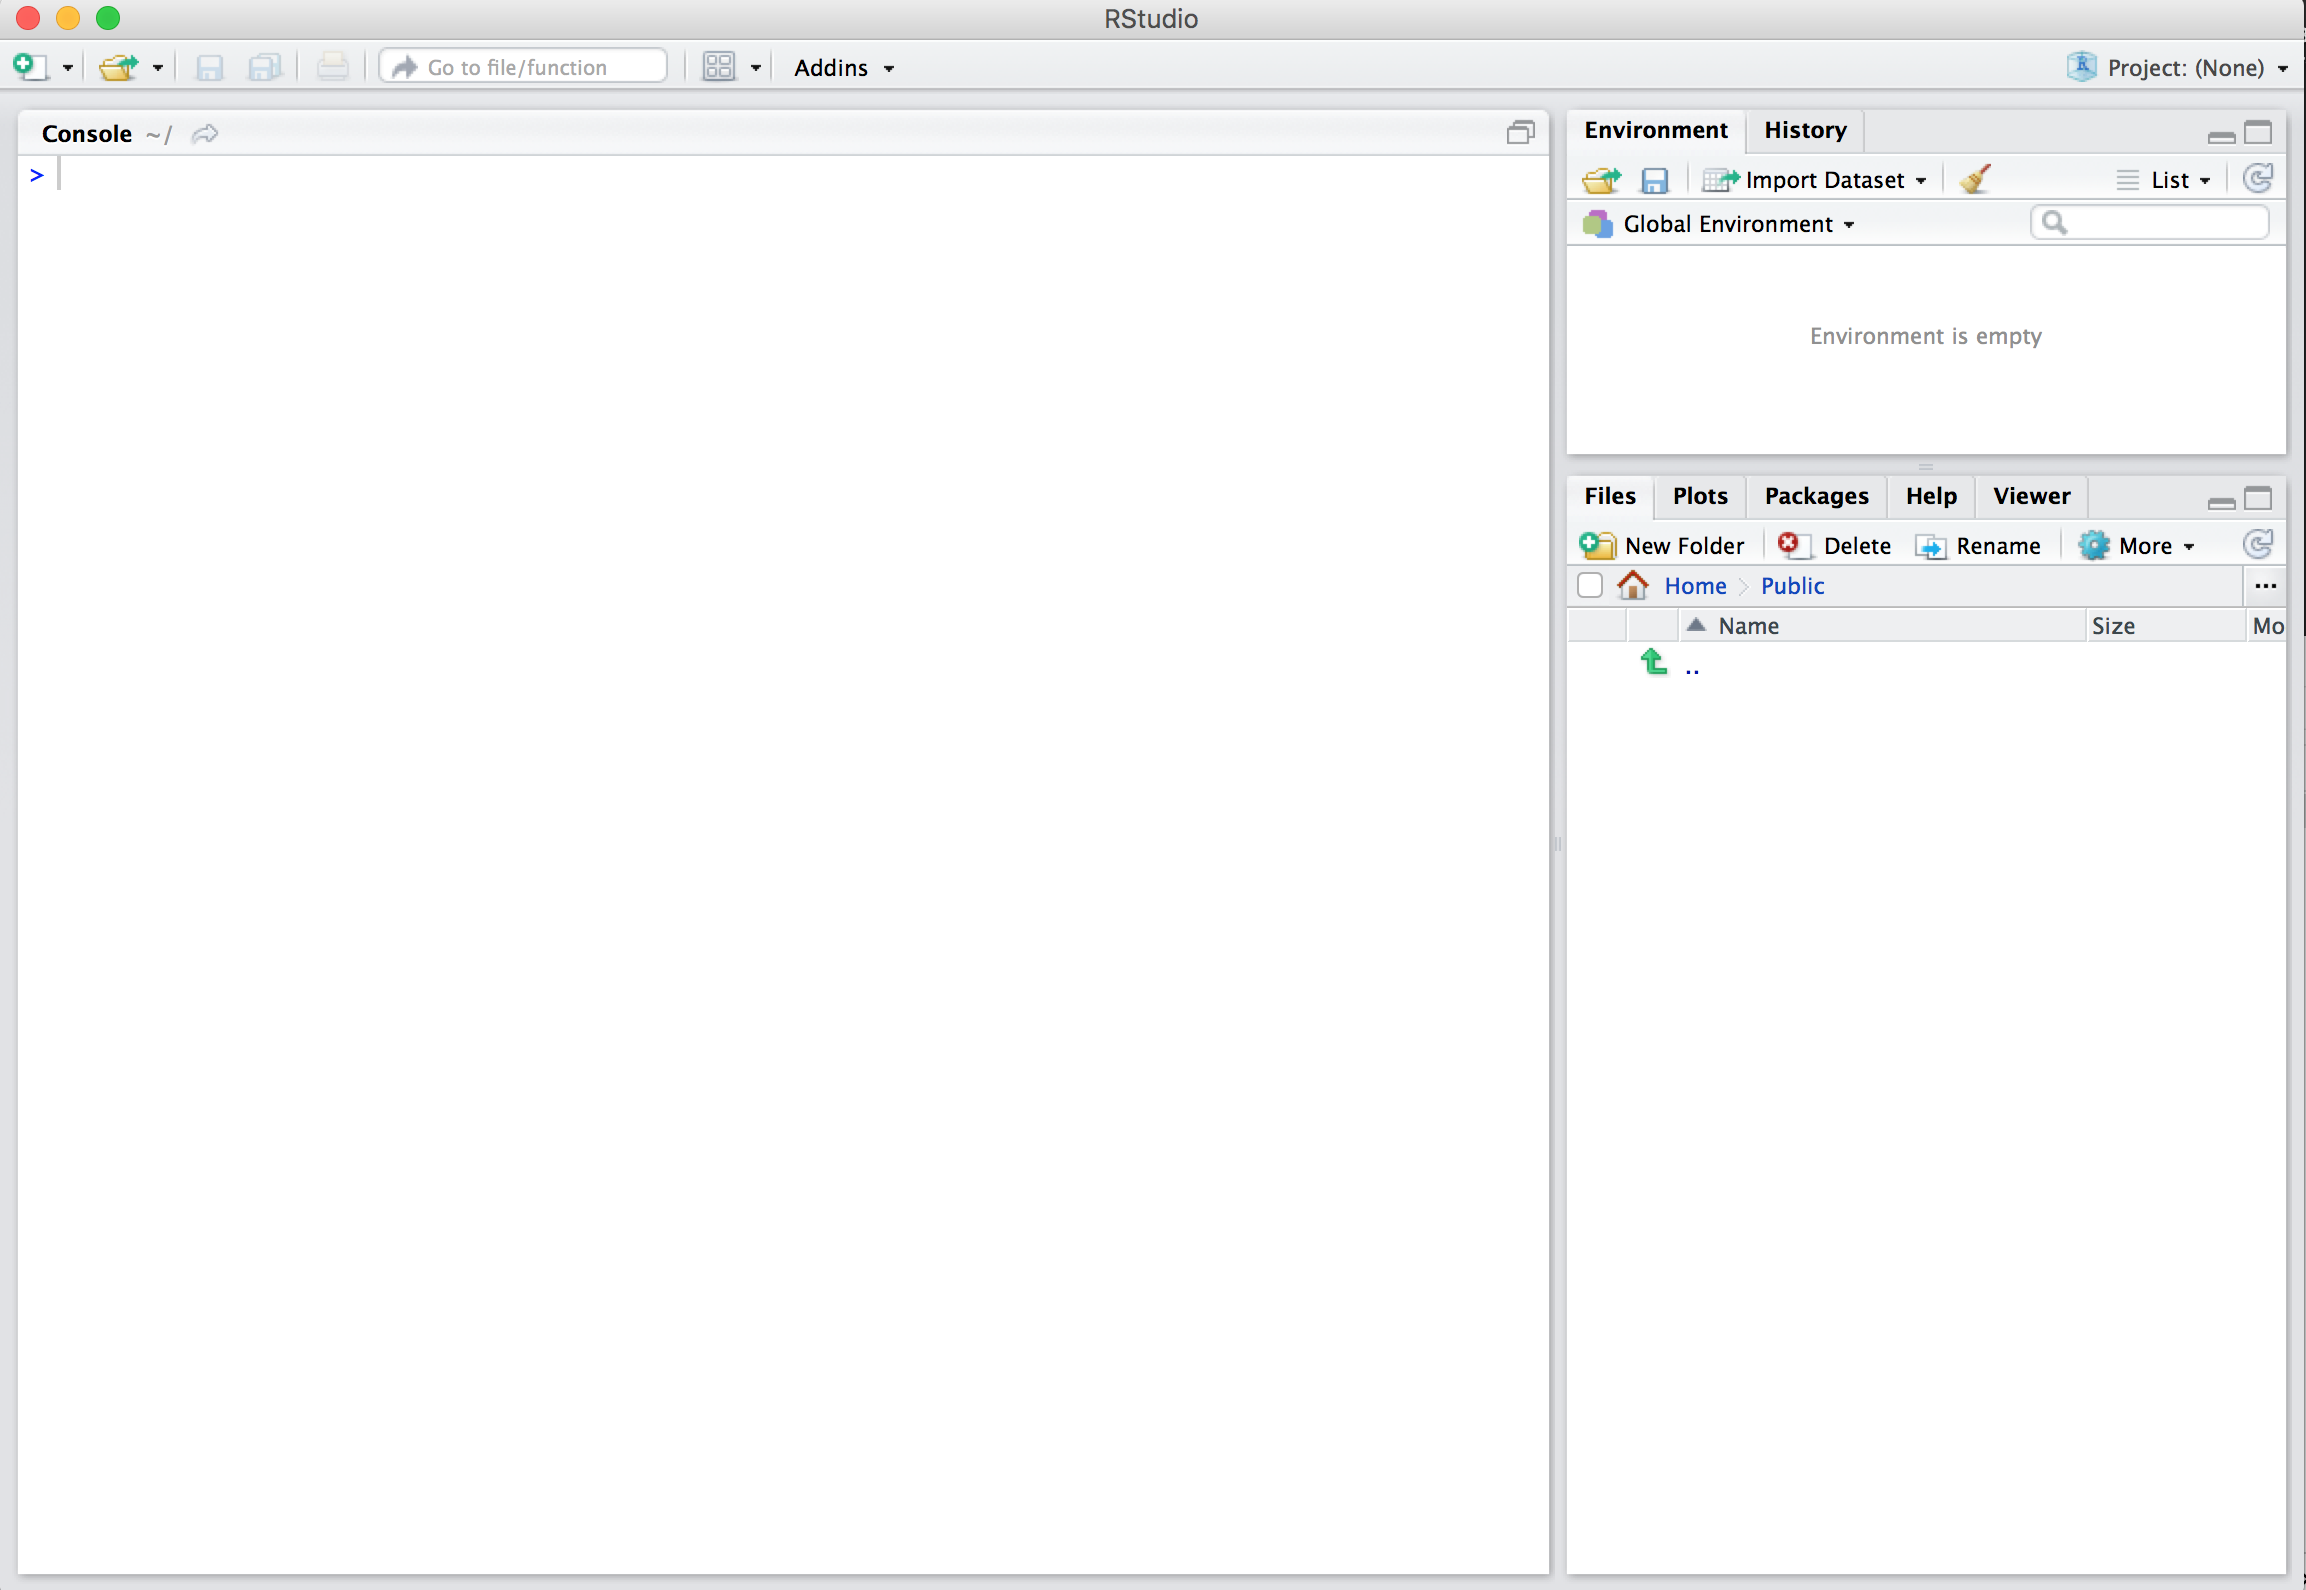
\includegraphics{./images/rstudio.png}

Prenez le temps d'explorer cette interface, cliquez sur les différents
onglets, ouvrez les menus, allez faire un tour dans les préférences du
logiciel pour découvrir les différents panneaux de l'application, en
particulier la Console dans laquelle nous exécuterons très bientôt du
code \texttt{R}.

\hypertarget{sec-code}{%
\section{\texorpdfstring{Comment exécuter du code \texttt{R}
?}{Comment exécuter du code R ?}}\label{sec-code}}

Contrairement à d'autres logiciels comme Excel, STATA ou SAS qui
fournissent des interfaces où tout se fait en cliquant avec sa souris,
\texttt{R} est un langage interprété, ce qui signifie que vous devez
taper des commandes, écrites en code \texttt{R}. C'est-à-dire que vous
devez \textbf{programmer} en \texttt{R} (j'utilise les termes ``coder''
et ``programmer'' de manière interchangeable dans ce livre).

Il n'est pas nécessaire d'être un programmeur pour utiliser \texttt{R},
néanmoins, il est nécessaire de programmer ! Il existe en effet un
ensemble de concepts de programmation de base que les utilisateurs
\texttt{R} doivent comprendre et maîtriser. Par conséquent, bien que ce
livre ne soit pas un livre sur la programmation, vous en apprendrez
juste assez sur ces concepts de programmation de base pour explorer et
analyser efficacement des données.

\hypertarget{la-console}{%
\subsection{La console}\label{la-console}}

La façon la plus simple d'interagir avec \texttt{RStudio} (mais pas du
tout la meilleure !) consiste à taper directement des commandes que
\texttt{R} pourra comprendre \textbf{dans la Console}.

Cliquez dans la console (après le symbole \texttt{\textgreater{}}) et
tapez ceci, sans oublier de valider en tapant sur la touche
\texttt{Entrée} :

\begin{Shaded}
\begin{Highlighting}[]
\DecValTok{3} \SpecialCharTok{+} \DecValTok{8}
\end{Highlighting}
\end{Shaded}

\begin{verbatim}
[1] 11
\end{verbatim}

Félicitations, vous venez de taper votre première instruction \texttt{R}
: vous savez maintenant faire des additions !

Dans la version en ligne de ce livre (en html), à chaque fois que du
code \texttt{R} sera fourni, il apparaîtra dans un cadre grisé avec une
ligne bleue à gauche, comme ci-dessus. Vous pourrez toujours taper dans
\texttt{RStudio}, les commandes qui figurent dans ces blocs de code,
afin d'obtenir vous même les résultats souhaités. Dans ce livre, lorsque
les commandes \texttt{R} produisent des résultats, ils sont affichés
juste en dessous des blocs de code. Enfin, en passant la souris sur les
blocs de code, vous verrez apparaître, à droite, une icône de
presse-papier qui vous permettra de copier-coller les commandes du livre
dans la console de \texttt{RStudio} ou, très bientôt, dans vos scripts.

\begin{tcolorbox}[enhanced jigsaw, bottomtitle=1mm, title=\textcolor{quarto-callout-warning-color}{\faExclamationTriangle}\hspace{0.5em}{Les risques du ``copier-coller'' {\faIcon{regular}}}, breakable, opacitybacktitle=0.6, coltitle=black, opacityback=0, toprule=.15mm, toptitle=1mm, titlerule=0mm, colback=white, rightrule=.15mm, arc=.35mm, leftrule=.75mm, bottomrule=.15mm, left=2mm, colframe=quarto-callout-warning-color-frame, colbacktitle=quarto-callout-warning-color!10!white]
Attention : il est fortement conseillé de réserver les copier-coller aux
blocs de commandes de (très) grande taille, ou en cas d'erreur de
syntaxe inexplicable. L'expérience a en effet montré qu'\textbf{on
apprend beaucoup mieux {en tapant soi-même les commandes}}. Ça n'est que
comme cela que l'on peut prendre conscience de toutes les subtilités du
langage (par exemple, faut-il mettre une virgule ou un point, une
parenthèse ou un crochet, le symbole moins ou un tilde, etc.). Je vous
conseille donc de taper vous-même les commandes autant que possible.
\end{tcolorbox}

\hypertarget{sec-script}{%
\subsection{Les scripts}\label{sec-script}}

Taper du code directement dans la console est probablement la pire façon
de travailler dans \texttt{RStudio}. Cela est parfois utile pour faire
un rapide calcul, ou pour vérifier qu'une commande fonctionne
correctement. Mais la plupart du temps, \textbf{vous devriez taper vos
commandes dans un script}.

\begin{tcolorbox}[enhanced jigsaw, bottomtitle=1mm, title=\textcolor{quarto-callout-important-color}{\faExclamation}\hspace{0.5em}{Définition importante !}, breakable, opacitybacktitle=0.6, coltitle=black, opacityback=0, toprule=.15mm, toptitle=1mm, titlerule=0mm, colback=white, rightrule=.15mm, arc=.35mm, leftrule=.75mm, bottomrule=.15mm, left=2mm, colframe=quarto-callout-important-color-frame, colbacktitle=quarto-callout-important-color!10!white]

Un script est un fichier au format ``texte brut'' (cela signifie qu'il
n'y a pas de mise en forme et que ce fichier peut-être ouvert par
n'importe quel éditeur de texte, y compris les plus simples comme le
bloc notes de Windows), dans lequel vous pouvez taper :

\begin{enumerate}
\def\labelenumi{\arabic{enumi}.}
\tightlist
\item
  des instructions qui seront comprises par \texttt{R} comme si vous les
  tapiez directement dans la console
\item
  des lignes de commentaires, qui doivent obligatoirement commencer par
  le symbole \texttt{\#}.
\end{enumerate}

\end{tcolorbox}

Les avantages de travailler dans un script sont nombreux :

\begin{enumerate}
\def\labelenumi{\arabic{enumi}.}
\tightlist
\item
  Vous pouvez sauvegarder votre script à tout moment (vous devriez
  prendre l'habitude de le sauvegarder très régulièrement). Vous gardez
  ainsi la trace de toutes les commandes que vous avez tapées.
\item
  Vous pouvez aisément partager votre script pour collaborer avec vos
  collègues de promo et enseignants.
\item
  Vous pouvez documenter votre démarche et les différentes étapes de vos
  analyses. \textbf{Vous devez ajouter autant de commentaires que
  possible}. Cela permettra à vos collaborateurs de comprendre ce que
  vous avez fait. Et dans 6 mois, cela vous permettra de comprendre ce
  que vous avez fait. Si votre démarche vous paraît cohérente
  aujourd'hui, il n'est en effet pas garanti que vous vous souviendrez
  de chaque détail quand vous vous re-plongerez dans vos analyses dans
  quelques temps. Donc aidez-vous vous même en commentant vos scripts
  dès maintenant.
\item
  Un script bien structuré, bien indenté (avec les bons retours à la
  ligne, des sauts de lignes, des espaces, bref, de l'air) et clair
  permet de rendre vos analyses répétables. Si vous passez 15 heures à
  analyser un tableau de données précis, il vous suffira de quelques
  secondes pour analyser un nouveau jeu de données similaire : vous
  n'aurez que quelques lignes à modifier dans votre script original pour
  l'appliquer à de nouvelles données.
\end{enumerate}

Vous pouvez créer un script en cliquant dans le menu ``File
\textgreater{} New File \textgreater{} R Script''. Un nouveau panneau
s'ouvre dans l'application. Pensez à sauvegarder immédiatement votre
nouveau script en cliquant dans le menu ``File \textgreater{} Save'' ou
``File \textgreater{} Save as\ldots{}''. Il faut pour cela lui donner un
nom et choisir un emplacement sur votre disque dur.

\begin{tcolorbox}[enhanced jigsaw, bottomtitle=1mm, title=\textcolor{quarto-callout-important-color}{\faExclamation}\hspace{0.5em}{Où sauvegarder vos scripts ? {\faIcon{regular}}}, breakable, opacitybacktitle=0.6, coltitle=black, opacityback=0, toprule=.15mm, toptitle=1mm, titlerule=0mm, colback=white, rightrule=.15mm, arc=.35mm, leftrule=.75mm, bottomrule=.15mm, left=2mm, colframe=quarto-callout-important-color-frame, colbacktitle=quarto-callout-important-color!10!white]
Je vous encourage vivement à créer, sur votre disque dur, un nouveau
dossier spécifique, que vous nommerez par exemple \texttt{BiometrieS3}.
Il est important que le nom de ce dossier de contienne pas de caractères
spéciaux (\emph{e.g.} accents, cédilles, apostrophes, espaces, etc.). Ce
dossier devrait être facilement accessible : vous y enregistrerez tous
vos scripts, vos jeux de données, vos graphiques, etc.

Si vous travaillez sur les ordinateurs de l'université, créez
{obligatoirement} votre dossier sur le disque
\texttt{W:\textbackslash{}}. Il s'agit de votre espace personnel sur le
réseau de l'université. Cela vous garantit que vous retrouverez votre
script la prochaine fois, même si vous utilisez un ordinateur différent.
\end{tcolorbox}

À partir de maintenant, vous ne devriez plus taper de commande
directement dans la console. Tapez systématiquement vos commandes dans
un script et sauvegardez-le régulièrement.

Pour exécuter les commandes du script dans la console, il suffit de
placer le curseur sur la ligne contenant la commande et de presser les
touches \texttt{ctrl\ +\ enter} (ou \texttt{command\ +\ enter} sous
macOS). Si un message d'erreur s'affiche dans la console, c'est que
votre instruction était erronée. Modifiez la directement dans votre
script et pressez à nouveau les touches \texttt{ctrl\ +\ enter} (ou
\texttt{command\ +\ enter} sous macOS) pour tenter à nouveau votre
chance. Idéalement, votre script ne devrait contenir que des commandes
qui fonctionnent et des commentaires expliquant à quoi servent ces
commandes.

Voici un exemple de script que je ne vous demande pas de reproduire.
Lisez simplement attentivement son contenu :

\begin{Shaded}
\begin{Highlighting}[]
\CommentTok{\# Penser à installer le package ggplot2 si besoin}
\CommentTok{\# install.packages("ggplot2")}

\CommentTok{\# Chargement du package}
\FunctionTok{library}\NormalTok{(ggplot2)}

\CommentTok{\# Mise en mémoire des données de qualité de l\textquotesingle{}air à New{-}York de mai à}
\CommentTok{\# septembre 1973}
\FunctionTok{data}\NormalTok{(airquality)}

\CommentTok{\# Affichage des premières lignes du tableau de données}
\FunctionTok{head}\NormalTok{(airquality)}

\CommentTok{\# Quelle est la structure de ce tableau ?}
\FunctionTok{str}\NormalTok{(airquality)}

\CommentTok{\# Réalisation d\textquotesingle{}un graphique présentant la relation entre la concentration}
\CommentTok{\# en ozone atmosphérique en ppb et la température en degrés Farenheit}
\FunctionTok{ggplot}\NormalTok{(}\AttributeTok{data =}\NormalTok{ airquality, }\AttributeTok{mapping =} \FunctionTok{aes}\NormalTok{(}\AttributeTok{x =}\NormalTok{ Temp, }\AttributeTok{y =}\NormalTok{ Ozone)) }\SpecialCharTok{+}
  \FunctionTok{geom\_point}\NormalTok{() }\SpecialCharTok{+}
  \FunctionTok{geom\_smooth}\NormalTok{(}\AttributeTok{method =} \StringTok{"loess"}\NormalTok{)}

\CommentTok{\# On constate une augmentation importante de la concentration d\textquotesingle{}ozone }
\CommentTok{\# pour des températures supérieures à 75ºF}
\end{Highlighting}
\end{Shaded}

Même si vous ne comprenez pas encore les commandes qui figurent dans ce
script (ça viendra !), voici ce que vous devez en retenir :

\begin{enumerate}
\def\labelenumi{\arabic{enumi}.}
\tightlist
\item
  Le script contient plus de lignes de commentaires que de commandes
  \texttt{R}.
\item
  Chaque étape de l'analyse est décrite en détail.
\item
  Les 2 dernières lignes du script décrivent les résultats obtenus (ici,
  un graphique).
\item
  Seules des commandes pertinentes et qui fonctionnent ont été
  conservées dans ce script.
\item
  Chaque ligne de commentaire commence par \texttt{\#}. Il est ainsi
  possible de conserver certaines commandes \texttt{R} dans le script,
  ``pour mémoire'', sans pour autant qu'elle ne soient exécutées. C'est
  le cas pour la ligne \texttt{\#\ install.packages("ggplot2")}.
\end{enumerate}

Si j'exécute ce script dans la console de \texttt{RStudio} (en
sélectionnant toutes les lignes et en pressant les touches
\texttt{ctrl\ +\ enter} ou \texttt{command\ +\ enter} sous macOS), voilà
ce qui est produit :

\begin{verbatim}
  Ozone Solar.R Wind Temp Month Day
1    41     190  7.4   67     5   1
2    36     118  8.0   72     5   2
3    12     149 12.6   74     5   3
4    18     313 11.5   62     5   4
5    NA      NA 14.3   56     5   5
6    28      NA 14.9   66     5   6
\end{verbatim}

\begin{verbatim}
'data.frame':   153 obs. of  6 variables:
 $ Ozone  : int  41 36 12 18 NA 28 23 19 8 NA ...
 $ Solar.R: int  190 118 149 313 NA NA 299 99 19 194 ...
 $ Wind   : num  7.4 8 12.6 11.5 14.3 14.9 8.6 13.8 20.1 8.6 ...
 $ Temp   : int  67 72 74 62 56 66 65 59 61 69 ...
 $ Month  : int  5 5 5 5 5 5 5 5 5 5 ...
 $ Day    : int  1 2 3 4 5 6 7 8 9 10 ...
\end{verbatim}

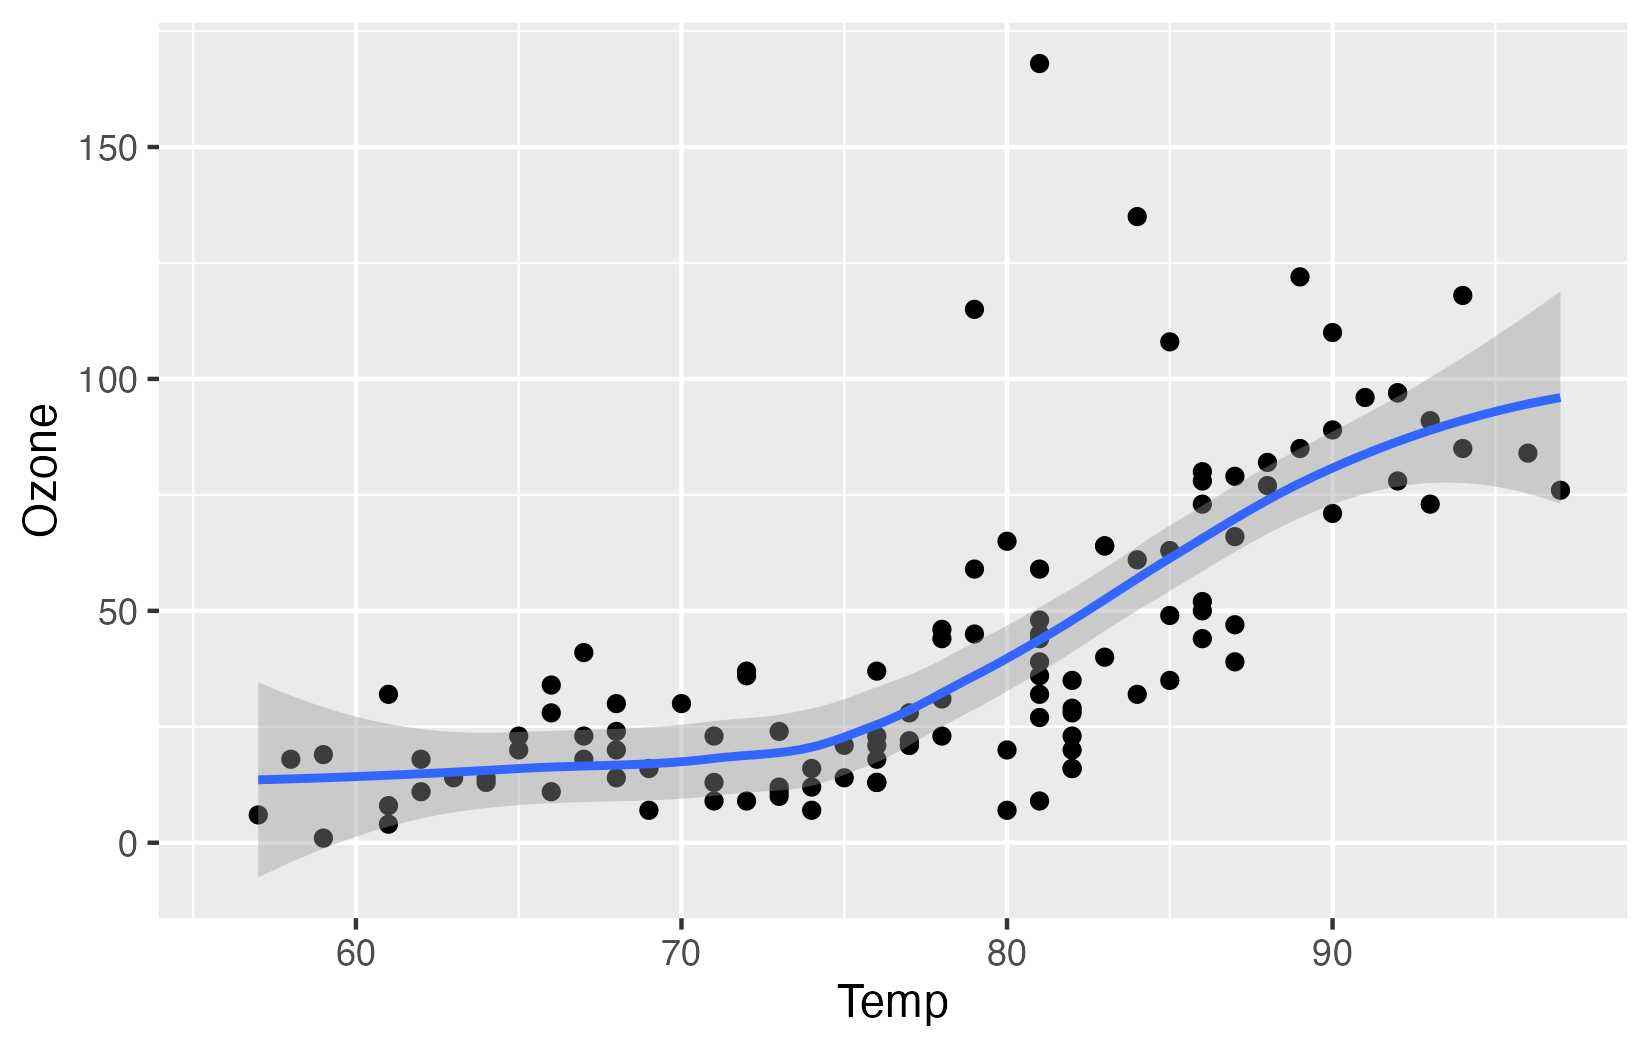
\includegraphics{./01-R-basics_files/figure-pdf/unnamed-chunk-3-1.png}

\hypertarget{les-projets-ou-rprojects}{%
\subsection{\texorpdfstring{Les projets, ou
\texttt{Rprojects}}{Les projets, ou Rprojects}}\label{les-projets-ou-rprojects}}

Pour travailler le plus efficacement possible avec \texttt{RStudio},
vous devriez créer, à l'intérieur de votre dossier de travail, un
nouveau fichier très particulier, qui s'appelle, dans le jargon de
\texttt{RStudio}, un \textbf{\texttt{Rproject}}.

Pour le créer, cliquez simplement dans le Menu ``File \textgreater{} New
Project\ldots{}''. Cette boîte de dialogue devrait apparaître :

\begin{figure}

{\centering 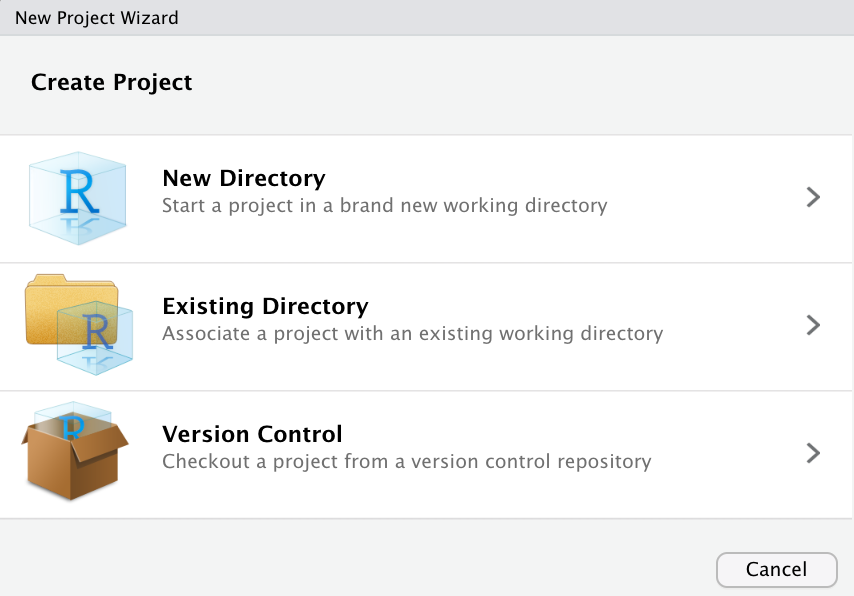
\includegraphics[width=0.6\textwidth,height=\textheight]{./images/Rproj1.png}

}

\end{figure}

Choisissez ``Existing Directory'', puis, dans la boîte de dialogue
suivante :

\begin{figure}

{\centering 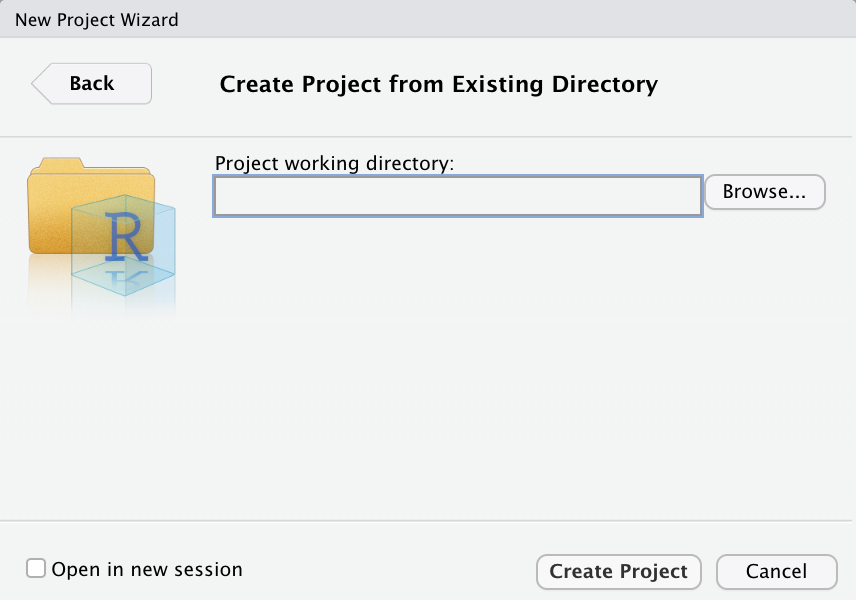
\includegraphics[width=0.6\textwidth,height=\textheight]{./images/Rproj2.png}

}

\end{figure}

cliquez sur ``Browse\ldots{}'', naviguez jusqu'au dossier que vous avez
créé plus tôt sur votre disque dur et qui contient votre script, puis
cliquez sur ``Create Project''. La fenêtre de \texttt{RStudio} se ferme,
puis une nouvelle fenêtre vierge apparaît. En apparence, rien n'a changé
ou presque. Pourtant :

\begin{enumerate}
\def\labelenumi{\arabic{enumi}.}
\tightlist
\item
  en haut à droite de la fenêtre de \texttt{RStudio}, le logiciel
  indique maintenant que vous êtes bel et bien à l'intérieur d'un
  \texttt{Rproject}. Au lieu de \texttt{Project:\ (None)}, on lit
  maintenant le nom du \texttt{Rproject} (chez moi,
  \texttt{BiometrieS3})
\item
  dans le quart inférieur droit de l'interface, l'onglet ``Files'' ne
  présente plus le même aspect. Avant de créer le \texttt{Rproject}, cet
  onglet présentait le chemin vers le dossier utilisé par défaut par le
  logiciel, ainsi que son contenu. Il s'agissait d'un dossier système
  auquel il vaut mieux ne pas toucher pour éviter les problèmes. Après
  la création du \texttt{Rproject}, l'onglet ``Files'' indique le
  contenu du dossier contenant le projet. Autrement dit, c'est ici que
  vous trouverez vos scripts, tableaux de données dans différents
  formats, figures sauvegardées, etc. Dans cet onglet, vous pouvez donc
  cliquer sur le nom de votre script pour l'ouvrir à nouveau, le
  modifier, l'exécuter\ldots{}
\end{enumerate}

\begin{figure}

\begin{minipage}[t]{0.50\linewidth}

{\centering 

\raisebox{-\height}{

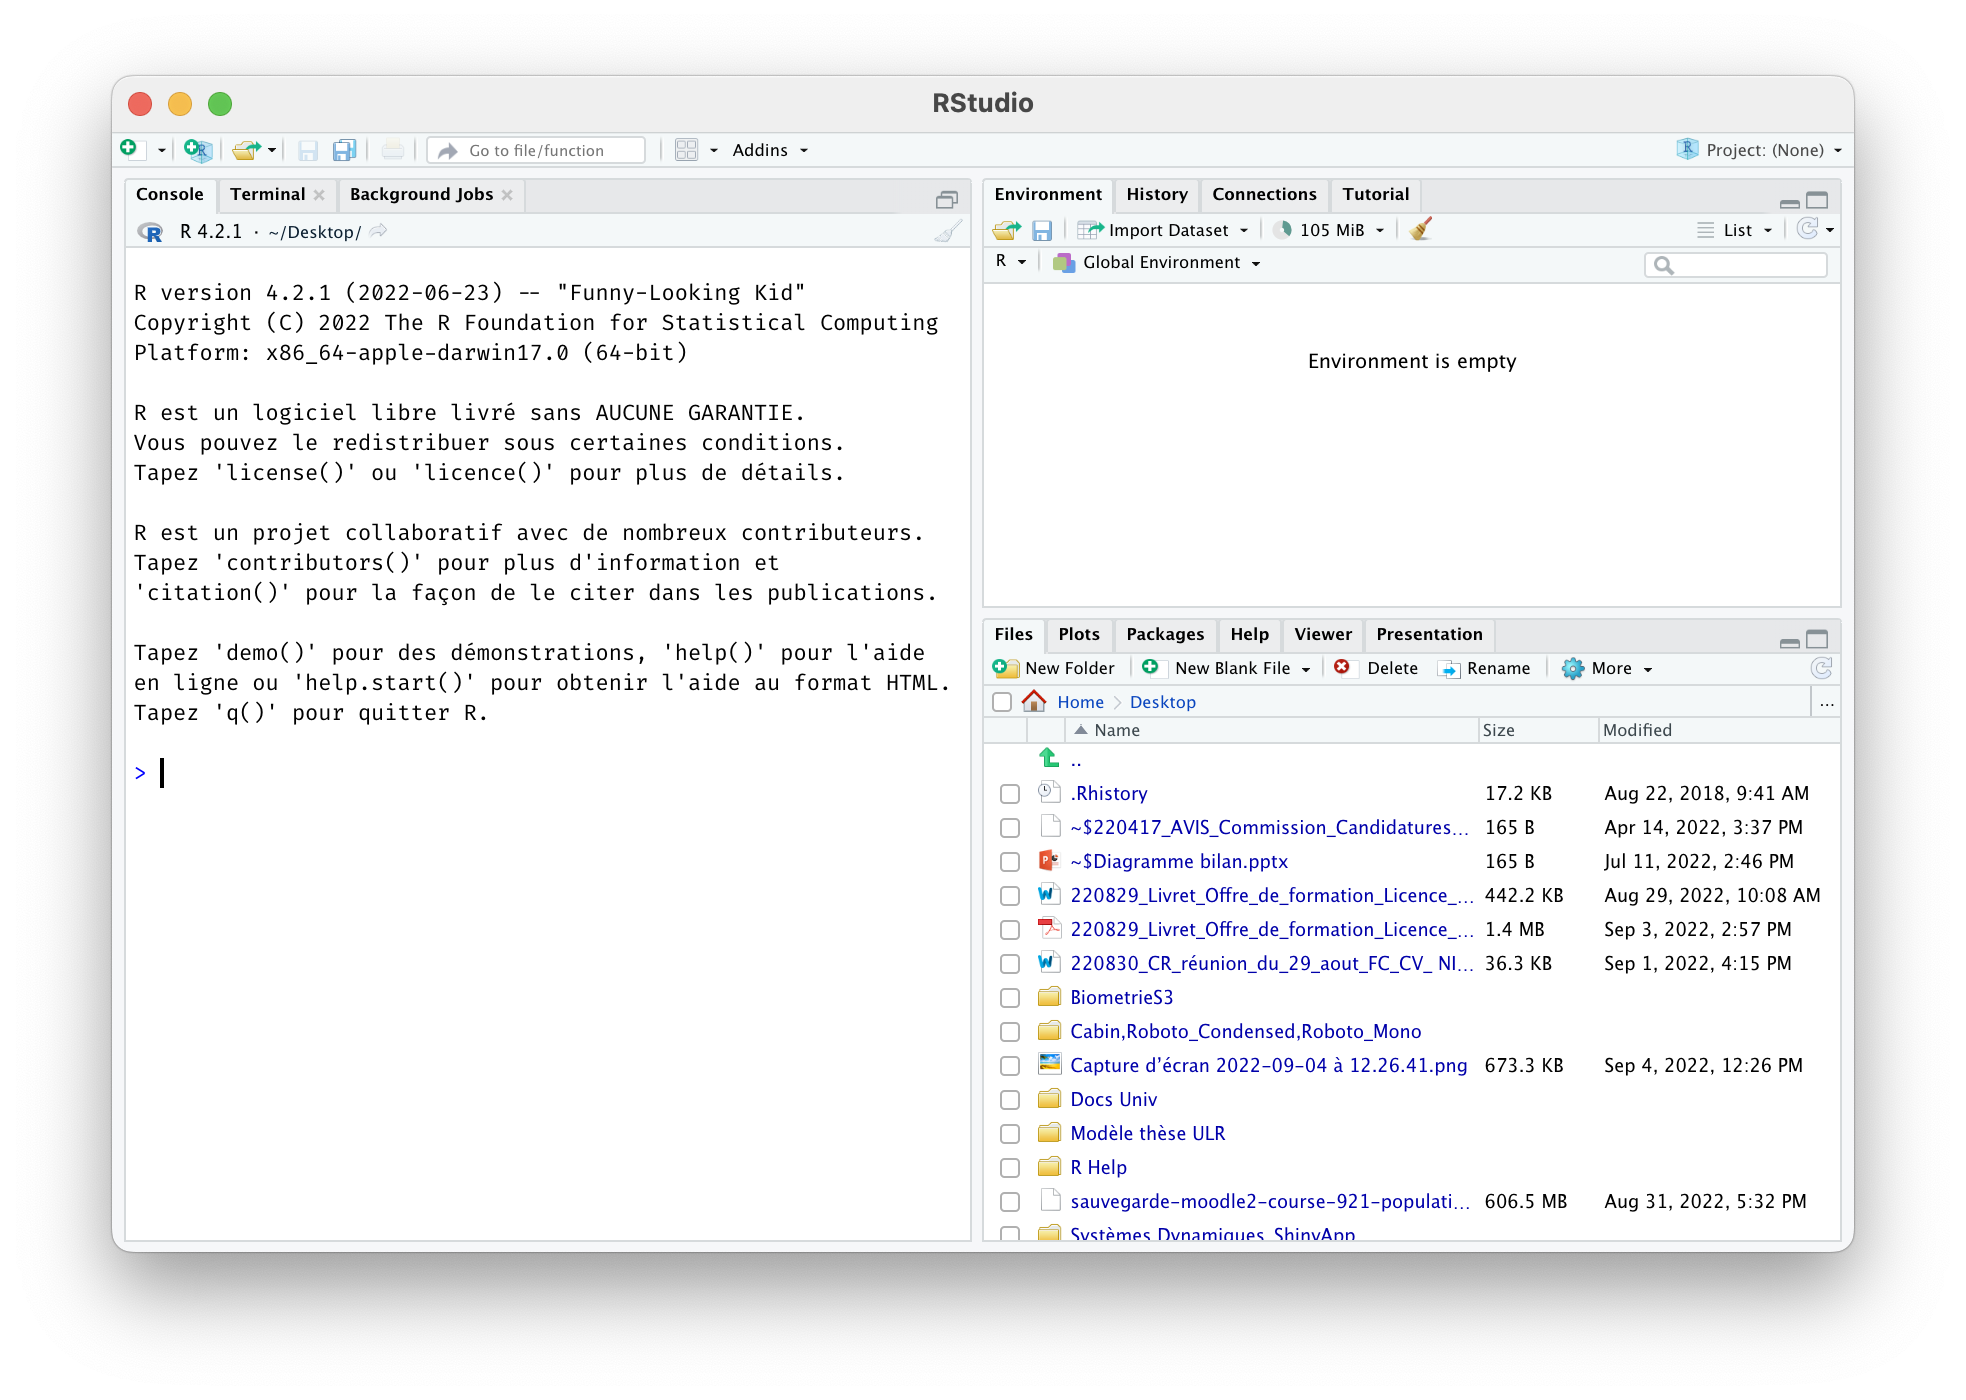
\includegraphics{./images/Avant.png}

}

\caption{Sans \texttt{Rproject}}

}

\end{minipage}%
%
\begin{minipage}[t]{0.50\linewidth}

{\centering 

\raisebox{-\height}{

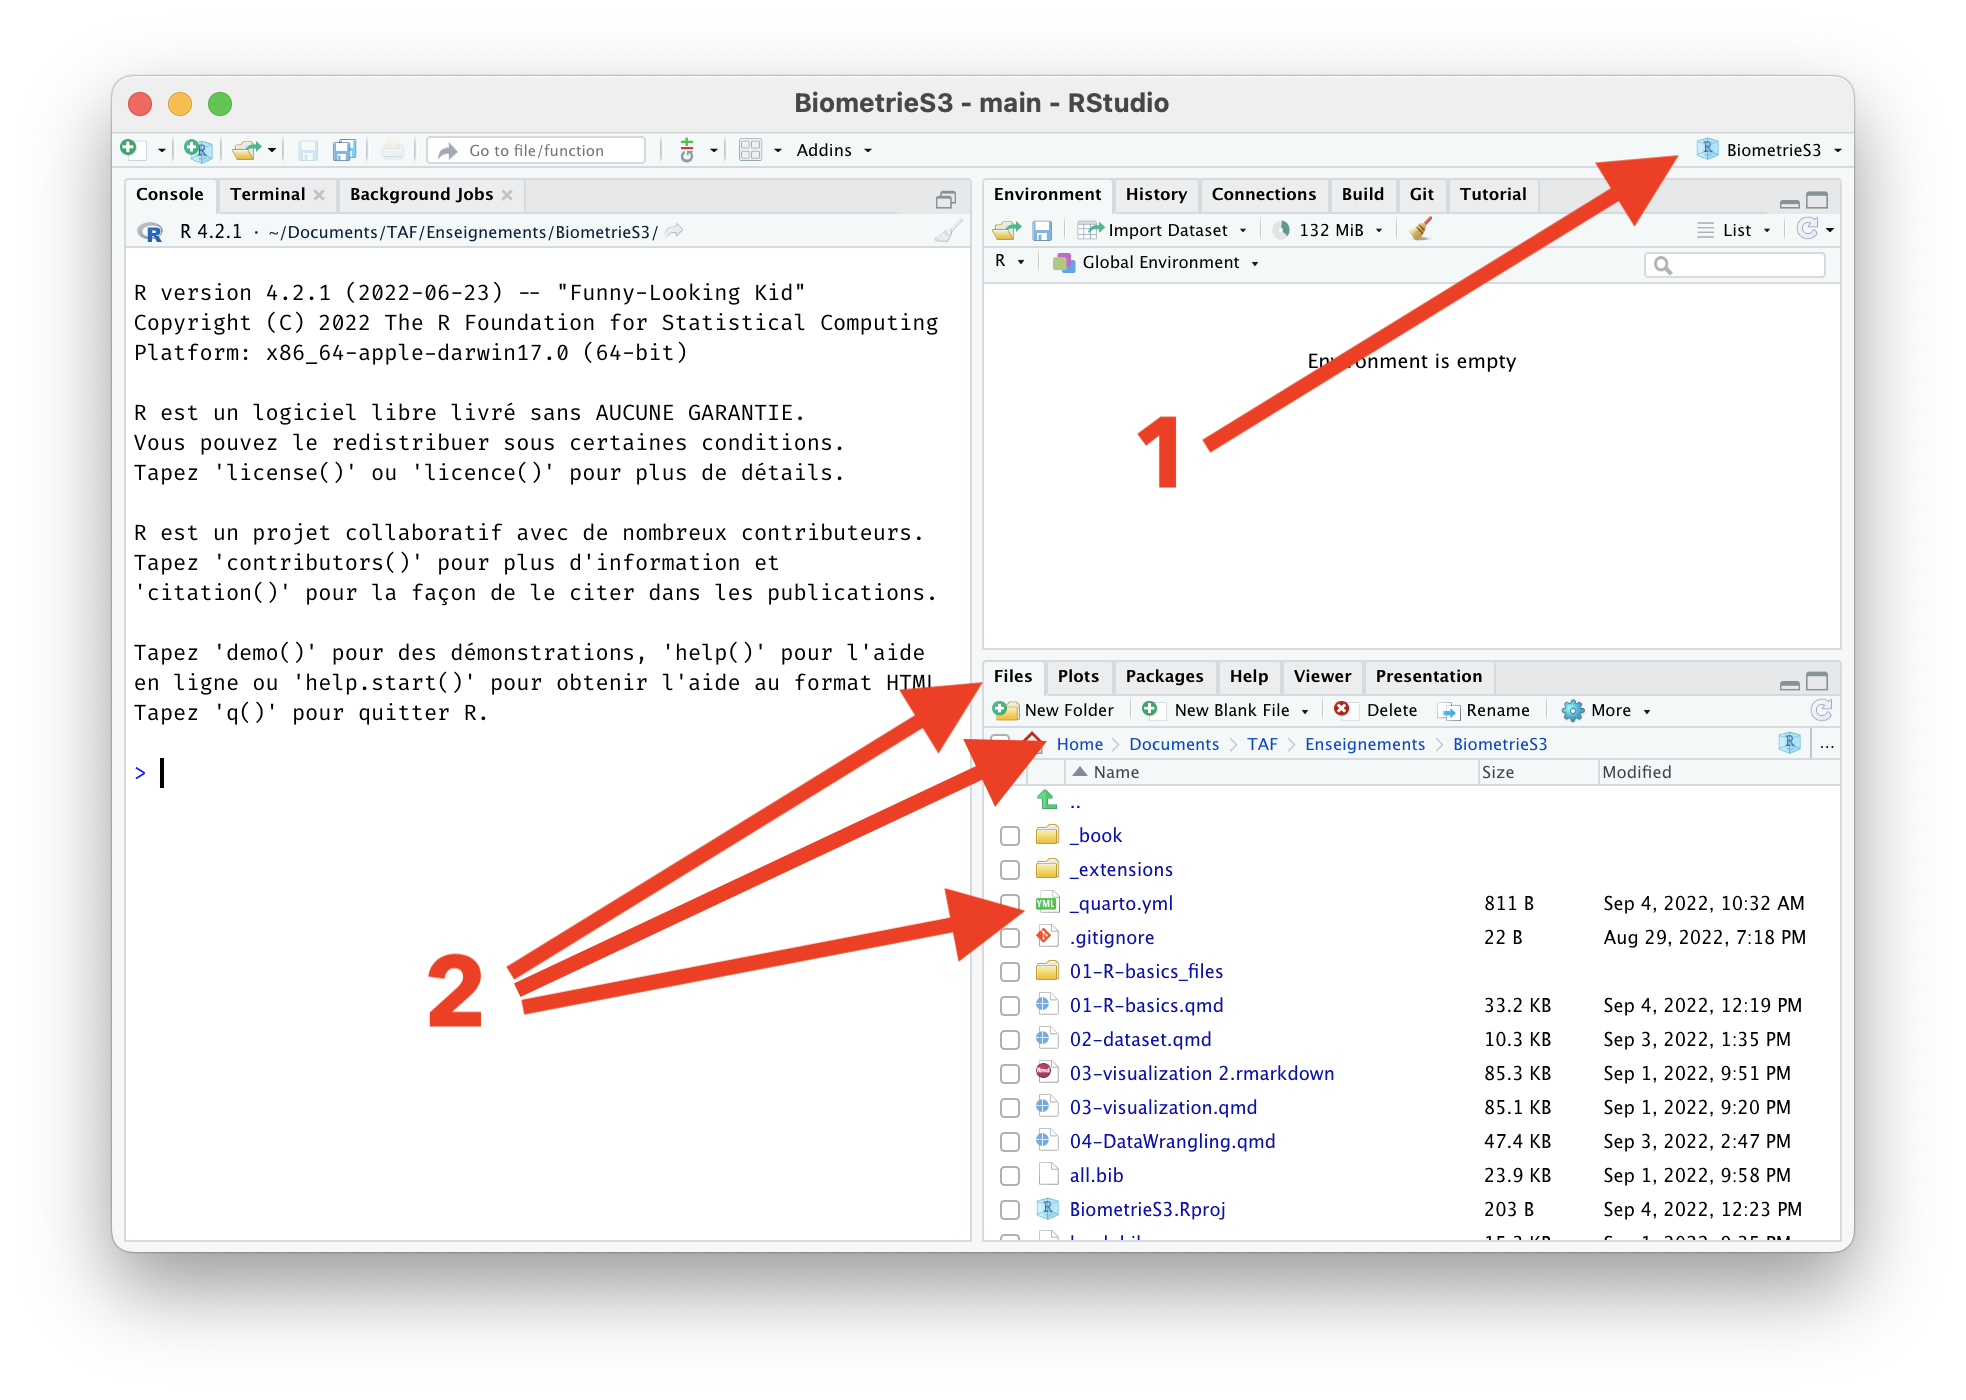
\includegraphics{./images/Après.png}

}

\caption{Avec \texttt{RProject}}

}

\end{minipage}%

\end{figure}

\begin{enumerate}
\def\labelenumi{\arabic{enumi}.}
\setcounter{enumi}{2}
\tightlist
\item
  un nouveau fichier portant l'extension \texttt{.rproj} a été créé dans
  votre dossier de travail. La prochaine fois que vous voudrez
  travailler dans \texttt{RStudio}, il vous suffira de double-cliquer
  sur ce fichier dans l'explorateur de fichier de Windows ou le Finder
  de MacOS, pour que \texttt{RStudio} s'ouvre, et que vous retrouviez
  tous vos fichiers et scripts de la fois précédente
\end{enumerate}

\begin{figure}

{\centering 
\includegraphics[width=0.2\textwidth,height=\textheight]{./images/Rproj3.png}

}

\end{figure}

Pour vérifier que tout s'est bien passé jusqu'ici, tapez la commande
suivante dans votre script puis envoyez-la dans la console en pressant
les touches \texttt{ctrl\ +\ entrée} (ou \texttt{command\ +\ entrée}
sous MacOS).

\begin{Shaded}
\begin{Highlighting}[]
\FunctionTok{getwd}\NormalTok{()}
\end{Highlighting}
\end{Shaded}

\texttt{RStudio} doit vous afficher, dans la console, le chemin jusqu'à
votre {répertoire de travail} ou ``Working Directory'' en anglais
(\texttt{getwd()} est l'abréviation de ``GET Working Directory''). Si
tout s'est bien passé, ce chemin doit être celui du dossier qui contient
votre script et le fichier \texttt{.Rproj} que vous venez de créer. Si
ce n'est pas le cas, reprenez calmement toutes les étapes décrites
depuis le début de la Section~\ref{sec-script}. Si ça ne fonctionne
toujours pas, contactez-moi sur Slack.

\begin{tcolorbox}[enhanced jigsaw, bottomtitle=1mm, title=\textcolor{quarto-callout-important-color}{\faExclamation}\hspace{0.5em}{Pour résumer\ldots{} \faIcon{computer}}, breakable, opacitybacktitle=0.6, coltitle=black, opacityback=0, toprule=.15mm, toptitle=1mm, titlerule=0mm, colback=white, rightrule=.15mm, arc=.35mm, leftrule=.75mm, bottomrule=.15mm, left=2mm, colframe=quarto-callout-important-color-frame, colbacktitle=quarto-callout-important-color!10!white]
Les \texttt{Rprojects} sont un moyen très pratique de travailler
efficacement dans \texttt{RStudio} car ils permettent de gérer
facilement la question du répertoire de travail. Lorsque vous envisagez
de travailler sur un nouveau sujet/projet/jeu de données/compte-rendu de
TP\ldots, les étapes à suivre, pour vous mettre dans une configuration
idéale qui vous évitera bien des problèmes par la suite, sont donc les
suivantes :

\begin{enumerate}
\def\labelenumi{\arabic{enumi}.}
\tightlist
\item
  Sur votre ordinateur, créez un nouveau dossier avec un nom simple, et
  à un endroit facile d'accès (pas de caractères spéciaux dans le chemin
  du dossier si possible)
\item
  Démarrez \texttt{RStudio}
\item
  Dans le logiciel, cliquez dans le menu ``File \textgreater{} New
  Project\ldots{}''
\item
  Choisissez ``Existing Directory'', puis naviguez jusqu'au dossier que
  vous venez de créer
\item
  Cliquez sur ``Create Project''
\item
  Créer un nouveau script (menu ``File \textgreater{} New File
  \textgreater{} R script'')
\item
  Donnez un nom à votre script (menu ``File \textgreater{} Save
  As\ldots{}'') pour le sauvegarder. Par défaut, \texttt{RStudio} vous
  propose d'enregistrer votre script dans le dossier de votre
  \texttt{Rproject}, ce qui est parfait.
\item
  Tapez \texttt{getwd()} dans votre script et exécutez cette commande en
  l'envoyant dans la console.
\end{enumerate}

Si le chemin qui s'affiche est celui du dossier contenant votre
\texttt{Rproject} et votre script, félicitation, vous êtes prêt·e à
travailler. Avec un peu d'habitude, ces étapes ne prennent qu'une à deux
minutes.
\end{tcolorbox}

\hypertarget{concepts-de-base-en-programmation-et-terminologie}{%
\subsection{Concepts de base en programmation et
terminologie}\label{concepts-de-base-en-programmation-et-terminologie}}

Après ces considérations techniques sur l'utilisation et les réglages de
\texttt{RStudio}, nous entrons maintenant dans le vif du sujet avec la
découverte des premiers éléments de syntaxe du langage \texttt{R}.

\hypertarget{sec-objects}{%
\subsubsection{Objets, types, vecteurs, facteurs et tableaux de
données}\label{sec-objects}}

Pour vous présenter les concepts de base et la terminologie de la
programmation dont nous aurons besoin, vous allez suivre des tutoriels
en ligne sur le site de DataCamp. Pour cette première prise en main,
tout va maintenant se passer dans votre navigateur internet, et vous
pouvez donc mettre de côté \texttt{RStudio} pour l'instant. Vous allez
voir que l'interface de DataCamp ressemble à une version simplifiée de
l'éditeur de script et de la console de \texttt{RStudio} : vous n'aurez
pas à vous soucier des réglages, de \texttt{Rprojects} ou de sauvegarder
quoi que ce soit. Si vous avez correctement créé votre compte gratuit
DataCamp comme indiqué au tout début de la Chapitre~\ref{sec-bases},
votre progression sera sauvegardée automatiquement. Il vous suffit de
cliquer sur les liens direct ci-dessous pour démarrer les tutoriels en
ligne.

Avant de démarrer, quelques précisions :

\begin{itemize}
\tightlist
\item
  pour chaque tutoriel que je vous demande de suivre, j'indique
  ci-dessous une liste des concepts de programmation qui sont couverts.
  N'hésitez pas à vous y référer (et à y revenir) tout au long du
  semestre si vous avez oublié certaines choses
\item
  ce tutoriel DataCamp contient 6 chapitres. Seuls les chapitres 1, 2,
  4, et 5 doivent être suivis. Nous ne travaillerons pas sur les
  matrices ni sur les listes
\item
  à la fin de chaque chapitre du tutoriel, revenez à ce livre en ligne
  pour cliquer sur le lien direct ver le chapitre suivant. Procéder
  ainsi vous évitera de suivre des chapitres inutiles du tutoriel, et
  cela vous permettra également d'éviter les demandes d'inscriptions
  payantes à DataCamp
\end{itemize}

Il est important de noter que, bien que ces tutoriels sont d'excellentes
introductions, une lecture seule, même attentive, est insuffisante pour
un apprentissage en profondeur et une rétention à long terme. Il faut
pour cela \textbf{pratiquer} et \textbf{répéter}. Outre les exercices
demandés dans DataCamp, que vous devez effectuer directement dans votre
navigateur, je vous encourage à prendre des notes, à multiplier les
essais, directement dans la console de \texttt{RStudio}, ou, de
préférence, dans un script que vous annoterez, pour vous assurer que
vous avez bien compris chaque partie.

Allez maintenant découvrir
\href{https://www.datacamp.com/community/open-courses/introduction-a-r}{le
cours d'introduction à R} sur DataCamp, et cliquez sur les liens des
chapitres ci-dessous. Au fur et à mesure de votre travail, notez les
termes importants et ce à quoi ils font référence.

\begin{itemize}
\tightlist
\item
  \href{https://campus.datacamp.com/courses/introduction-a-r/chapitre-1-introduction?ex=1}{Chapitre
  1 : introduction}

  \begin{itemize}
  \tightlist
  \item
    La console : l'endroit où vous tapez des commandes
  \item
    Les objets : où les valeurs sont stockées, comment assigner des
    valeurs à des objets
  \item
    Les types de données : entiers, doubles/numériques, caractères et
    logiques
  \end{itemize}
\item
  \href{https://campus.datacamp.com/courses/introduction-a-r/chapitre-2-les-vecteurs?ex=1}{Chapitre
  2 : vecteurs}

  \begin{itemize}
  \tightlist
  \item
    Les vecteurs : des collections de valeurs du même type
  \end{itemize}
\item
  \href{https://campus.datacamp.com/courses/introduction-a-r/chapitre-4-facteurs?ex=1}{Chapitre
  4 : les facteurs}

  \begin{itemize}
  \tightlist
  \item
    Des données catégorielles (et non pas \emph{numériques})
    représentées dans \texttt{R} sous forme de \texttt{factor}s
  \end{itemize}
\item
  \href{https://campus.datacamp.com/courses/introduction-a-r/chapitre-5-les-jeux-de-donnees?ex=1}{Chapitre
  5 : les jeux de données ou \texttt{data.frame}}

  \begin{itemize}
  \tightlist
  \item
    Les \texttt{data.frame}s sont similaires aux feuilles de calcul
    rectangulaires que l'on peut produire dans un tableur. Dans
    \texttt{R}, ce sont des objets rectangulaires (des tableaux !)
    contenant des jeux de données : les lignes correspondent aux
    observations et les colonnes aux variables décrivant les
    observations. La plupart du temps, c'est le format de données que
    nous utiliserons. Plus de détails dans le Chapitre~\ref{sec-dataset}
  \end{itemize}
\end{itemize}

Avant de passer à la suite, il nous reste 2 grandes notions à découvrir
dans le domaine du code et de la syntaxe afin de pouvoir travailler
efficacement dans \texttt{R} : les opérateurs de comparaison d'une part,
et les fonctions d'autre part. Pour les découvrir et expérimenter, et
puisque vous avez terminé les tutoriels DataCamp, reprenez maintenant
\texttt{RStudio} et travaillez dans votre script.

\hypertarget{sec-comparaison}{%
\subsubsection{Opérateurs de comparaison}\label{sec-comparaison}}

Comme leur nom l'indique, ils permettent de comparer des valeurs ou des
objets. Les principaux opérateurs de comparaison sont :

\begin{itemize}
\tightlist
\item
  \texttt{==} : égal à
\item
  \texttt{!=} : différent de
\item
  \texttt{\textgreater{}} : supérieur à
\item
  \texttt{\textless{}} : inférieur à
\item
  \texttt{\textgreater{}=} : supérieur ou égal à
\item
  \texttt{\textless{}=} : inférieur ou égal à
\end{itemize}

Ainsi, on peut tester si 3 est égal à 5 :

\begin{Shaded}
\begin{Highlighting}[]
\DecValTok{3} \SpecialCharTok{==} \DecValTok{5}
\end{Highlighting}
\end{Shaded}

\begin{verbatim}
[1] FALSE
\end{verbatim}

La réponse est bien entendu \texttt{FALSE}. Est-ce que 3 est inférieur à
5 ?

\begin{Shaded}
\begin{Highlighting}[]
\DecValTok{3} \SpecialCharTok{\textless{}} \DecValTok{5}
\end{Highlighting}
\end{Shaded}

\begin{verbatim}
[1] TRUE
\end{verbatim}

La réponse est maintenant \texttt{TRUE}. Lorsque l'on utilise un
opérateur de comparaison, la réponse est toujours soit vrai
(\texttt{TRUE}), soit faux (\texttt{FALSE}).

Il est aussi possible de comparer des chaînes de charactères :

\begin{Shaded}
\begin{Highlighting}[]
\StringTok{"Bonjour"} \SpecialCharTok{==} \StringTok{"Au revoir"}
\end{Highlighting}
\end{Shaded}

\begin{verbatim}
[1] FALSE
\end{verbatim}

\begin{Shaded}
\begin{Highlighting}[]
\StringTok{"Bonjour"} \SpecialCharTok{\textgreater{}=} \StringTok{"Au revoir"}
\end{Highlighting}
\end{Shaded}

\begin{verbatim}
[1] TRUE
\end{verbatim}

Manifestement, ``Bonjour'' est supérieur ou égal à ``Au revoir''. En
fait, \texttt{R} utilise l'ordre alphabétique pour comparer les chaînes
de caractères. Puisque dans l'alphabet, le ``B'' de ``Bonjour'' arrive
après le ``A'' de ``Au revoir'', pour \texttt{R}, ``Bonjour'' est
supérieur à ``Au revoir''.

Il est également possible d'utiliser ces opérateurs pour comparer un
chiffre et un vecteur :

\begin{Shaded}
\begin{Highlighting}[]
\NormalTok{tailles\_pop1 }\OtherTok{\textless{}{-}} \FunctionTok{c}\NormalTok{(}\DecValTok{112}\NormalTok{, }\DecValTok{28}\NormalTok{, }\DecValTok{86}\NormalTok{, }\DecValTok{14}\NormalTok{, }\DecValTok{154}\NormalTok{, }\DecValTok{73}\NormalTok{, }\DecValTok{63}\NormalTok{, }\DecValTok{48}\NormalTok{)}
\NormalTok{tailles\_pop1 }\SpecialCharTok{\textgreater{}} \DecValTok{80}
\end{Highlighting}
\end{Shaded}

\begin{verbatim}
[1]  TRUE FALSE  TRUE FALSE  TRUE FALSE FALSE FALSE
\end{verbatim}

Ici, l'opérateur nous permet d'identifier quels éléments du vecteur
\texttt{taille\_pop1} sont supérieurs à 80. Il s'agit des éléments
placés en première, troisième et cinquième positions.

Il est aussi possible de comparer 2 vecteurs qui contiennent le même
nombre d'éléments :

\begin{Shaded}
\begin{Highlighting}[]
\NormalTok{tailles\_pop2 }\OtherTok{\textless{}{-}} \FunctionTok{c}\NormalTok{(}\DecValTok{114}\NormalTok{, }\DecValTok{27}\NormalTok{, }\DecValTok{38}\NormalTok{, }\DecValTok{91}\NormalTok{, }\DecValTok{54}\NormalTok{, }\DecValTok{83}\NormalTok{, }\DecValTok{33}\NormalTok{, }\DecValTok{68}\NormalTok{)}
\NormalTok{tailles\_pop1 }\SpecialCharTok{\textgreater{}}\NormalTok{ tailles\_pop2}
\end{Highlighting}
\end{Shaded}

\begin{verbatim}
[1] FALSE  TRUE  TRUE FALSE  TRUE FALSE  TRUE FALSE
\end{verbatim}

Les comparaisons sont ici faites élément par élément. Ainsi, les
observations 2, 3, 5 et 7 du vecteur \texttt{tailles\_pop1} sont
supérieures aux observations 2, 3, 5 et 7 du vecteur
\texttt{tailles\_pop2} respectivement.

Ces vecteurs de vrais/faux sont très utiles car ils peuvent permettre de
compter le nombre d'éléments répondant à une certains condition :

\begin{Shaded}
\begin{Highlighting}[]
\FunctionTok{sum}\NormalTok{(tailles\_pop1 }\SpecialCharTok{\textgreater{}}\NormalTok{ tailles\_pop2)}
\end{Highlighting}
\end{Shaded}

\begin{verbatim}
[1] 4
\end{verbatim}

Lorsque l'on effectue une opération arithmétique (comme le calcul d'une
somme ou d'une moyenne) sur un vecteur de vrais/faux, les \texttt{TRUE}
sont remplacés par \texttt{1} et les \texttt{FALSE} par \texttt{0}. La
somme nous indique donc le nombre de vrais dans un vecteur de
vrais/faux, et la moyenne nous indique la proportion de vrais :

\begin{Shaded}
\begin{Highlighting}[]
\FunctionTok{mean}\NormalTok{(tailles\_pop1 }\SpecialCharTok{\textgreater{}}\NormalTok{ tailles\_pop2)}
\end{Highlighting}
\end{Shaded}

\begin{verbatim}
[1] 0.5
\end{verbatim}

\textbf{Note} : Attention, si les vecteurs comparés n'ont pas la même
taille, un message d'avertissement est affiché :

\begin{Shaded}
\begin{Highlighting}[]
\NormalTok{tailles\_pop3 }\OtherTok{\textless{}{-}} \FunctionTok{c}\NormalTok{(}\DecValTok{43}\NormalTok{, }\DecValTok{56}\NormalTok{, }\DecValTok{92}\NormalTok{)}
\NormalTok{tailles\_pop1}
\end{Highlighting}
\end{Shaded}

\begin{verbatim}
[1] 112  28  86  14 154  73  63  48
\end{verbatim}

\begin{Shaded}
\begin{Highlighting}[]
\NormalTok{tailles\_pop3}
\end{Highlighting}
\end{Shaded}

\begin{verbatim}
[1] 43 56 92
\end{verbatim}

\begin{Shaded}
\begin{Highlighting}[]
\NormalTok{tailles\_pop3 }\SpecialCharTok{\textgreater{}}\NormalTok{ tailles\_pop1}
\end{Highlighting}
\end{Shaded}

\begin{verbatim}
Warning in tailles_pop3 > tailles_pop1: la taille d'un objet plus long n'est pas
multiple de la taille d'un objet plus court
\end{verbatim}

\begin{verbatim}
[1] FALSE  TRUE  TRUE  TRUE FALSE  TRUE FALSE  TRUE
\end{verbatim}

Ici, \texttt{R} renvoie un résultat, accompagné d'un message
d'avertissement qui nous indique que tout ne s'est probablement pas
déroulé comme on le pensait. Dans un cas comme celui là, \texttt{R} va
en effet \emph{recycler} l'objet le plus court, ici
\texttt{tailles\_pop3} pour qu'une comparaison puisse être faite avec
chaque élément de l'objet le plus long (ici, \texttt{tailles\_pop1}).
Ainsi, 43 est comparé à 112, 56 est comparé à 28 et 92 est comparé à 86.
Puisque \texttt{tailles\_pop3} ne contient plus d'éléments, ils sont
recyclés, dans le même ordre : 43 est comparé à 14, 56 est comparé à
154, et ainsi de suite jusqu'à ce que tous les éléments de
\texttt{tailles\_pop1} aient été passés en revue.

Ce type de recyclage est très risqué car il est difficile de savoir ce
qui a été comparé avec quoi. En travaillant avec des tableaux plutôt
qu'avec des vecteurs, le problème est généralement évité puisque toutes
les colonnes d'un \texttt{data.frame} contiennent le même nombre
d'éléments.

\begin{tcolorbox}[enhanced jigsaw, bottomtitle=1mm, title=\textcolor{quarto-callout-warning-color}{\faExclamationTriangle}\hspace{0.5em}{Erreur ou avertissement ? \faIcon{bomb} ou \faIcon{triangle-exclamation}
?}, breakable, opacitybacktitle=0.6, coltitle=black, opacityback=0, toprule=.15mm, toptitle=1mm, titlerule=0mm, colback=white, rightrule=.15mm, arc=.35mm, leftrule=.75mm, bottomrule=.15mm, left=2mm, colframe=quarto-callout-warning-color-frame, colbacktitle=quarto-callout-warning-color!10!white]
Il ne faut pas confondre message d'erreur et message d'avertissement :

\begin{itemize}
\tightlist
\item
  Un message d'{erreur} commence généralement par \texttt{Error} ou
  \texttt{Erreur} et indique que \texttt{R} n'a pas compris ce que vous
  lui demandiez. Il n'a donc pas été en mesure de faire quoi que ce soit
  et votre commande n'a donc pas été exécutée. Vous devez absolument
  revenir à votre code et corriger la commande fautive car il y a fort à
  parier que si vous ne le faites pas, les commandes suivantes
  renverrons à leur tour un message d'erreur. Il est donc important de
  toujours revenir à la première erreur d'un script et de la corriger
  avant de passer à la suite.
\item
  Un message d'{avertissement} commence généralement par
  \texttt{Warning} et vous indique que quelque chose d'inhabituel, ou de
  ``non-optimal'' a été réalisé. Un résultat a été produit, mais
  peut-être n'est-il pas conforme à ce que vous attendiez. La prudence
  est donc requise.
\end{itemize}

Dans les deux cas, un message explique de façon plus ou moins claire ce
qui a posé problème. Progresser dans la maîtrise du logiciel et du
langage signifie en grande partie progresser dans la compréhension de la
signification de ces messages parfois obscures. Pour progresser, il faut
donc commencer par \textbf{lire attentivement ces messages}, et tenter
de comprendre ce qu'ils veulent dire.
\end{tcolorbox}

Dernière chose concernant les opérateurs de comparaison : la question
des données manquantes. Dans \texttt{R} les données manquantes sont
symbolisées par cette notation : \texttt{NA}, abréviation de ``Not
Available''. Le symbole \texttt{NaN} (comme ``Not a Number'') est
parfois aussi observé lorsque des opérations ont conduit à des
indéterminations. Mais c'est plus rare et la plupart du temps, les
\texttt{NaN}s peuvent être traités comme les \texttt{NA}s. L'un des
problèmes des données manquantes est qu'il est nécessaire de prendre des
précautions pour réaliser des comparaisons les impliquant :

\begin{Shaded}
\begin{Highlighting}[]
\DecValTok{3} \SpecialCharTok{==} \ConstantTok{NA}
\end{Highlighting}
\end{Shaded}

\begin{verbatim}
[1] NA
\end{verbatim}

On s'attend logiquement à ce que 3 ne soit pas considéré comme égal à
\texttt{NA}, et donc, on s'attend à obtenir \texttt{FALSE}. Pourtant, le
résultat est \texttt{NA}. La comparaison d'un élément quelconque à une
donnée manquante fournit toujours une donnée manquante : la comparaison
ne peut pas se faire, \texttt{R} n'a donc rien à retourner. C'est
également le cas aussi lorsque l'on compare deux valeurs manquantes :

\begin{Shaded}
\begin{Highlighting}[]
\ConstantTok{NA} \SpecialCharTok{==} \ConstantTok{NA}
\end{Highlighting}
\end{Shaded}

\begin{verbatim}
[1] NA
\end{verbatim}

C'est en fait assez logique. Imaginons que j'ignore l'âge de Pierre et
l'âge de Marie. Il n'y a aucune raison pour que leur âge soit le même,
mais il est tout à fait possible qu'il le soit. C'est impossible à
déterminer :

\begin{Shaded}
\begin{Highlighting}[]
\NormalTok{age\_Pierre }\OtherTok{\textless{}{-}} \ConstantTok{NA}
\NormalTok{age\_Marie }\OtherTok{\textless{}{-}} \ConstantTok{NA}
\NormalTok{age\_Pierre }\SpecialCharTok{==}\NormalTok{ age\_Marie}
\end{Highlighting}
\end{Shaded}

\begin{verbatim}
[1] NA
\end{verbatim}

Mais alors comment faire pour savoir si une valeur est manquante
puisqu'on ne peut pas utiliser les opérateurs de comparaison ? On
utilise la fonction \texttt{is.na()} :

\begin{Shaded}
\begin{Highlighting}[]
\FunctionTok{is.na}\NormalTok{(age\_Pierre)}
\end{Highlighting}
\end{Shaded}

\begin{verbatim}
[1] TRUE
\end{verbatim}

\begin{Shaded}
\begin{Highlighting}[]
\FunctionTok{is.na}\NormalTok{(tailles\_pop3)}
\end{Highlighting}
\end{Shaded}

\begin{verbatim}
[1] FALSE FALSE FALSE
\end{verbatim}

D'une façon générale, le point d'exclamation permet de signifier à
\texttt{R} que nous souhaitons obtenir le contraire d'une expression :

\begin{Shaded}
\begin{Highlighting}[]
\SpecialCharTok{!}\FunctionTok{is.na}\NormalTok{(age\_Pierre)}
\end{Highlighting}
\end{Shaded}

\begin{verbatim}
[1] FALSE
\end{verbatim}

\begin{Shaded}
\begin{Highlighting}[]
\SpecialCharTok{!}\FunctionTok{is.na}\NormalTok{(tailles\_pop3)}
\end{Highlighting}
\end{Shaded}

\begin{verbatim}
[1] TRUE TRUE TRUE
\end{verbatim}

Cette fonction nous sera très utile plus tard pour éliminer toutes les
lignes d'un tableau contenant des valeurs manquantes.

\hypertarget{sec-functions}{%
\subsubsection{L'utilisation des fonctions}\label{sec-functions}}

Dans \texttt{R}, les fonctions sont des objets particuliers qui
permettent d'effectuer des tâches très variées. Du calcul d'une moyenne
à la création d'un graphique, en passant par la réalisation d'analyses
statistiques complexes ou simplement l'affichage du chemin du répertoire
de travail, tout, dans \texttt{R}, repose sur l'utilisation de
fonctions. Vous en avez déjà vu un certain nombre :

\begin{longtable}[]{@{}
  >{\raggedleft\arraybackslash}p{(\columnwidth - 2\tabcolsep) * \real{0.2800}}
  >{\raggedright\arraybackslash}p{(\columnwidth - 2\tabcolsep) * \real{0.7200}}@{}}
\toprule()
\begin{minipage}[b]{\linewidth}\raggedleft
Fonction
\end{minipage} & \begin{minipage}[b]{\linewidth}\raggedright
Pour quoi faire ?
\end{minipage} \\
\midrule()
\endhead
\texttt{c()} & Créer des vecteurs \\
\texttt{class()} & Afficher ou modifier la classe d'un objet \\
\texttt{factor()} & Créer des facteurs \\
\texttt{getwd()} & Afficher le chemin du répertoire de travail \\
\texttt{head()} & Afficher les premiers éléments d'un objet \\
\texttt{is.na()} & Tester si un objet contient des valeurs manquantes \\
\texttt{mean()} & Calculer une moyenne \\
\texttt{names()} & Afficher ou modifier le nom des éléments d'un
vecteur \\
\texttt{order()} & Ordonner les éléments d'un objet \\
\texttt{subset()} & Extraire une partie des éléments d'un objet \\
\texttt{sum()} & Calculer une somme \\
\texttt{tail()} & Afficher les derniers éléments d'un objet \\
\bottomrule()
\end{longtable}

Cette liste va très rapidement s'allonger au fil des séances. Je vous
conseille donc vivement de tenir à jour une liste des fonctions
décrites, avec une explication de leur fonctionnement et éventuellement
un exemple de syntaxe.

Certaines fonctions ont besoin d'arguments (par exemple, la fonction
\texttt{factor()}), d'autres peuvent s'en passer (par exemple, la
fonction \texttt{getwd()}). Pour apprendre comment utiliser une fonction
particulière, pour découvrir quels sont ses arguments possibles, quel
est leur rôle et leur intérêt, la meilleure solution est de consulter
l'aide de cette fonction. Il suffit pour cela de taper un \texttt{?}
suivi du nom de la fonction :

\begin{Shaded}
\begin{Highlighting}[]
\NormalTok{?}\FunctionTok{factor}\NormalTok{()}
\end{Highlighting}
\end{Shaded}

Toutes les fonctions et jeux de données disponibles dans \texttt{R}
disposent d'un fichier d'aide similaire. Cela peut faire un peu peur au
premier abord (tout est en anglais !), mais ces fichiers d'aide ont
l'avantage d'être très complets, de fournir des exemples d'utilisation,
et ils sont tous construits sur le même modèle. Vous avez donc tout
intérêt à vous familiariser avec eux. Vous devriez d'ailleurs prendre
l'habitude de consulter l'aide de chaque fonction qui vous pose un
problème. Par exemple, le logarithme (en base 10) de 100 devrait faire
2, car 100 est égal à 10\^{}2. Pourtant :

\begin{Shaded}
\begin{Highlighting}[]
\FunctionTok{log}\NormalTok{(}\DecValTok{100}\NormalTok{)}
\end{Highlighting}
\end{Shaded}

\begin{verbatim}
[1] 4.60517
\end{verbatim}

Que se passe-t'il ? Pour le savoir, il faut consulter l'aide de la
fonction log :

\begin{Shaded}
\begin{Highlighting}[]
\NormalTok{?}\FunctionTok{log}\NormalTok{()}
\end{Highlighting}
\end{Shaded}

Ce fichier d'aide nous apprend que par défaut, la syntaxe de la fonction
\texttt{log()} est la suivante :

\begin{Shaded}
\begin{Highlighting}[]
\FunctionTok{log}\NormalTok{(x, }\AttributeTok{base =} \FunctionTok{exp}\NormalTok{(}\DecValTok{1}\NormalTok{))}
\end{Highlighting}
\end{Shaded}

Par défaut, la base du logarithme est fixée à \texttt{exp(1)}. Nous
avons donc calculé un logarithme népérien (en base \emph{e}). Cette
fonction prend donc 2 arguments :

\begin{enumerate}
\def\labelenumi{\arabic{enumi}.}
\tightlist
\item
  \texttt{x} ne possède pas de valeur par défaut : il nous faut
  obligatoirement fournir quelque chose (la rubrique ``Argument'' du
  fichier d'aide nous indique que \texttt{x} doit être un vecteur
  numérique ou complexe) afin que la fonction puisse calculer un
  logarithme
\item
  \texttt{base} possède un argument par défaut. Si nous ne spécifions
  pas nous même la valeur de \texttt{base}, elle sera fixée à sa valeur
  par défaut, c'est à dire \texttt{exp(1)}.
\end{enumerate}

Pour calculer le logarithme de 100 en base 10, il faut donc taper, au
choix, l'une de ces 3 expressions :

\begin{Shaded}
\begin{Highlighting}[]
\FunctionTok{log}\NormalTok{(}\AttributeTok{x =} \DecValTok{100}\NormalTok{, }\AttributeTok{base =} \DecValTok{10}\NormalTok{)}
\end{Highlighting}
\end{Shaded}

\begin{verbatim}
[1] 2
\end{verbatim}

\begin{Shaded}
\begin{Highlighting}[]
\FunctionTok{log}\NormalTok{(}\DecValTok{100}\NormalTok{, }\AttributeTok{base =} \DecValTok{10}\NormalTok{)}
\end{Highlighting}
\end{Shaded}

\begin{verbatim}
[1] 2
\end{verbatim}

\begin{Shaded}
\begin{Highlighting}[]
\FunctionTok{log}\NormalTok{(}\DecValTok{100}\NormalTok{, }\DecValTok{10}\NormalTok{)}
\end{Highlighting}
\end{Shaded}

\begin{verbatim}
[1] 2
\end{verbatim}

Le nom des arguments d'une fonction peut être omis tant que ses
arguments sont indiqués dans l'ordre attendu par la fonction (cet ordre
est celui qui est précisé à la rubrique ``Usage'' du fichier d'aide de
la fonction). Il est possible de modifier l'ordre des arguments d'une
fonction, mais il faut alors être parfaitement explicite et utiliser les
noms des arguments tels que définis dans le fichier d'aide.

Ainsi, pour calculer le logarithme de 100 en base 10, on ne peut pas
taper :

\begin{Shaded}
\begin{Highlighting}[]
\FunctionTok{log}\NormalTok{(}\DecValTok{10}\NormalTok{, }\DecValTok{100}\NormalTok{)}
\end{Highlighting}
\end{Shaded}

\begin{verbatim}
[1] 0.5
\end{verbatim}

car cela revient à calculer le logarithme de 10 en base 100. On peut en
revanche taper :

\begin{Shaded}
\begin{Highlighting}[]
\FunctionTok{log}\NormalTok{(}\AttributeTok{base =} \DecValTok{10}\NormalTok{, }\AttributeTok{x =} \DecValTok{100}\NormalTok{)}
\end{Highlighting}
\end{Shaded}

\begin{verbatim}
[1] 2
\end{verbatim}

\hypertarget{sec-packages}{%
\section{Les packages additionels}\label{sec-packages}}

Une source de confusion importante pour les nouveaux utilisateurs de
\texttt{R} est la notion de package. Les packages étendent les
fonctionnalités de \texttt{R} en fournissant des fonctions, des données
et de la documentation supplémentaires et peuvent être téléchargés
gratuitement sur Internet. Ils sont écrits par une communauté mondiale
d'utilisateurs de \texttt{R}. Par exemple, parmi les plus de 18000
packages disponibles à l'heure actuelle, nous utiliseront fréquemment :

\begin{itemize}
\tightlist
\item
  Le package \texttt{ggplot2} pour la visualisation des données dans le
  Chapitre~\ref{sec-viz}
\item
  Le package \texttt{dplyr} pour manipuler des tableaux de données dans
  le Chapitre~\ref{sec-wrangling}
\end{itemize}

Une bonne analogie pour les packages \texttt{R} : ils sont comme les
apps que vous téléchargez sur un téléphone portable. \texttt{R} est
comme un nouveau téléphone mobile. Il est capable de faire certaines
choses lorsque vous l'utilisez pour la première fois, mais il ne sait
pas tout faire. Les packages sont comme les apps que vous pouvez
télécharger dans l'App Store et Google Play. Pour utiliser un package,
comme pour utiliser Instagram, vous devez :

\begin{enumerate}
\def\labelenumi{\arabic{enumi}.}
\tightlist
\item
  Le télécharger et l'installer. Vous ne le faites qu'une fois grâce à
  la commande \texttt{install.packages()}
\item
  Le charger (en d'autres termes, l'ouvrir) en utilisant la commande
  \texttt{library()} à chaque nouvelle session de travail
\end{enumerate}

Donc, tout comme vous ne pouvez commencer à partager des photos avec vos
amis sur Instagram que si vous installez d'abord l'application et que
vous l'ouvrez, vous ne pouvez accéder aux données et fonctions d'un
package \texttt{R} que si vous installez d'abord le package et le
chargez avec la fonction \texttt{library()}. Passons en revue ces 2
étapes.

\hypertarget{installation-dun-package}{%
\subsection{Installation d'un package}\label{installation-dun-package}}

Il y a deux façons d'installer un package. Par example, pour installer
le package \texttt{ggplot2} :

\begin{enumerate}
\def\labelenumi{\arabic{enumi}.}
\tightlist
\item
  \textbf{Le plus simple} : Dans le quart inférieur droit de l'interface
  de \texttt{Rstudio} :

  \begin{enumerate}
  \def\labelenumii{\alph{enumii})}
  \tightlist
  \item
    Cliquez sur l'onglet ``Packages''
  \item
    Cliquez sur ``Install''
  \item
    Tapez le nom du package dans le champ ``Packages (separate multiple
    with space or comma):'' Pour notre exemple, tapez \texttt{ggplot2}
  \item
    Cliquez sur ``Install''
  \end{enumerate}
\item
  \textbf{Métode alternative} : Dans la console, tapez
  \texttt{install.packages("ggplot2")} (vous devez inclure les
  guillemets).
\end{enumerate}

En procédant de l'une ou l'autre façon, installez également les packages
suivants : \texttt{tidyverse} et \texttt{palmerpenguins}. Le
\texttt{tidyverse} est un ``méta-package'', qui permet en fait
d'installer de nombreux packages en une seule commande, dont
\texttt{ggplot2}, \texttt{tidyr}, \texttt{dplyr}, \texttt{magrittr} et
bien d'autres. Le package \texttt{palmerpenguins} contient un jeu de
données dont nous nous servirons copieusement dans les chapitres
suivants.

\begin{tcolorbox}[enhanced jigsaw, bottomtitle=1mm, title=\textcolor{quarto-callout-note-color}{\faInfo}\hspace{0.5em}{Note : \texttt{install.packages()}}, breakable, opacitybacktitle=0.6, coltitle=black, opacityback=0, toprule=.15mm, toptitle=1mm, titlerule=0mm, colback=white, rightrule=.15mm, arc=.35mm, leftrule=.75mm, bottomrule=.15mm, left=2mm, colframe=quarto-callout-note-color-frame, colbacktitle=quarto-callout-note-color!10!white]
Un package doit être installé une fois seulement sur un ordinateur, sauf
si une version plus récente est disponible et que vous souhaitez mettre
à jour ce package. Il n'est donc pas nécessaire de laisser ces commandes
dans votre script. Sinon, vous risquez de ré-installer les packages à
chaque nouvelle session de travail, ce qui est inutile et consomme
inutilement de la bande passante, des ressources numériques, et donc, du
carbone\ldots{} \faIcon{temperature-three-quarters}
\faIcon{earth-americas}
\end{tcolorbox}

\hypertarget{charger-un-package-en-muxe9moire}{%
\subsection{Charger un package en
mémoire}\label{charger-un-package-en-muxe9moire}}

Après avoir installé un package, vous pouvez le charger en utilisant la
fonction \texttt{library()}. Par exemple, pour charger \texttt{ggplot2}
et \texttt{dplyr} tapez ceci dans la console :

\begin{Shaded}
\begin{Highlighting}[]
\FunctionTok{library}\NormalTok{(ggplot2)}
\FunctionTok{library}\NormalTok{(dplyr)}
\end{Highlighting}
\end{Shaded}

Puisque ces packages font partie du \texttt{tidyverse}, on aurait pu les
charger tous les deux (et d'autres) en une seule étape en tapant :

\begin{Shaded}
\begin{Highlighting}[]
\FunctionTok{library}\NormalTok{(tidyverse)}
\end{Highlighting}
\end{Shaded}

Quand vous exécutez une commande, si vous voyez un message d'erreur
commençant par :

\begin{verbatim}
Error: could not find function...
\end{verbatim}

c'est probablement parce que vous tentez d'utiliser une fonction qui
fait partie d'un package que vous n'avez pas chargé. Pour corriger
l'erreur, il suffit donc de charger le package approprié avec la
commande \texttt{library()}.

\begin{tcolorbox}[enhanced jigsaw, bottomtitle=1mm, title=\textcolor{quarto-callout-note-color}{\faInfo}\hspace{0.5em}{Note : \texttt{library()}}, breakable, opacitybacktitle=0.6, coltitle=black, opacityback=0, toprule=.15mm, toptitle=1mm, titlerule=0mm, colback=white, rightrule=.15mm, arc=.35mm, leftrule=.75mm, bottomrule=.15mm, left=2mm, colframe=quarto-callout-note-color-frame, colbacktitle=quarto-callout-note-color!10!white]
Vous devrez charger à nouveau chaque package que vous souhaitez utiliser
\textbf{à chaque fois que vous ouvrirez une nouvelle session de travail
dans \texttt{RStudio}} (à chaque nouveau démarrage du logiciel, donc).
C'est une erreur fréquente pour les débutants. Pour l'éviter, pensez
bien à intégrer, tout en haut de votre script, les commandes
\texttt{library()} nécessaires pour chaque package que vous comptez
utiliser.
\end{tcolorbox}

\hypertarget{sec-Exo-1}{%
\section{Exercice}\label{sec-Exo-1}}

Dans votre dossier de travail, créez un nouveau script que vous nommerez
\texttt{ExoDiamonds.R}. Vous prendrez soin d'ajouter autant de
commentaires que nécessaire dans votre script afin de le structurer
correctement.

\begin{enumerate}
\def\labelenumi{\arabic{enumi}.}
\tightlist
\item
  Téléchargez (si besoin) et chargez le package \texttt{ggplot2}
\item
  Chargez le jeu de données \texttt{diamonds} grâce à la commande
  \texttt{data(diamonds)}
\item
  Déterminez le nombre de lignes et de colonnes de ce tableau nommé
  \texttt{diamonds}
\item
  Créez un nouveau tableau que vous nommerez \texttt{diamants\_chers}
  qui contiendra uniquement les informations des diamants dont le prix
  est supérieur ou égal à \$15000.
\item
  Combien de diamants coûtent \$15000 ou plus ?
\item
  Cela représente quelle proportion du jeu de données de départ ?
\item
  Triez ce tableau par ordre de prix décroissants et affichez les
  informations des 20 diamants les plus chers.
\end{enumerate}

\bookmarksetup{startatroot}

\hypertarget{sec-dataset}{%
\chapter{Explorez votre premier jeu de données}\label{sec-dataset}}

\hypertarget{pruxe9ambule-1}{%
\section{Préambule}\label{pruxe9ambule-1}}

Mettons en pratique tout ce que nous avons appris pour commencer à
explorer un jeu de données réel. Les données nous parviennent sous
différents formats, des images au texte en passant par des tableaux de
chiffres. Tout au long de ce document, nous nous concentrerons sur les
ensembles de données qui peuvent être stockés dans une feuille de
calcul, car il s'agit de la manière la plus courante de collecter des
données dans de nombreux domaines. N'oubliez pas ce que nous avons
appris dans la Section~\ref{sec-objects} : ces ensembles de données de
type ``tableurs'' sont appelés \texttt{data.frame} dans \texttt{R}, et
nous nous concentrerons sur l'utilisation de ces objets tout au long de
ce livre. S'il est évidemment possible d'importer dans \texttt{R} des
données stockées dans des fichiers Excel ou des fichiers textes, nous
allons dans un premier temps faire plus simple : nous travaillerons avec
des données déjà disponibles dans un packages que nous avons installé
dans la Section~\ref{sec-packages}.

Ainsi, commençons par charger les packages nécessaires pour ce chapitre
(cela suppose que vous les ayez déjà installés ; relisez la
Section~\ref{sec-packages} pour plus d'informations sur l'installation
et le chargement des packages \texttt{R} si vous ne l'avez pas déjà
fait). Au début de chaque chapitre, nous aurons systématiquement besoin
de charger quelques packages. Donc n'oubliez pas de les installer au
préalable si besoin.

\begin{Shaded}
\begin{Highlighting}[]
\CommentTok{\# Pensez à installer ces packages avant de les charger si besoin }
\FunctionTok{library}\NormalTok{(dplyr)}
\FunctionTok{library}\NormalTok{(palmerpenguins)}
\end{Highlighting}
\end{Shaded}

\begin{center}\rule{0.5\linewidth}{0.5pt}\end{center}

\hypertarget{le-package-palmerpenguins}{%
\section{\texorpdfstring{Le package
\texttt{palmerpenguins}}{Le package palmerpenguins}}\label{le-package-palmerpenguins}}

Ce package (Horst, Hill, et Gorman 2022) contient un jeu de données
collectées par Kristen Gorman (membre du ``Long Term Ecological Research
Network'\,') et la station de Palmer en Antarctique (Gorman, Williams,
et Fraser 2014). Les données contiennent des informations au sujet de
330 individus appartenant à 3 espèces de manchots (voir
figure\textasciitilde{}\ref{ppenguins}) étudiés sur 3 îles de l'archipel
de Palmer, an Antarctique. Ces espèces ont fait l'objet de nombreuses
études comparatives, notamment afin de déterminer comment elles
utilisent le milieu pour acquérir des ressources. Puisque ces 3 espèces
sont proches sur le plan phylogénétique et qu'elles occupent le même
habitat, la question de la compétition inter-spécifique, pour l'espace
et les ressources, se pose tout naturellement.

\begin{figure}

{\centering 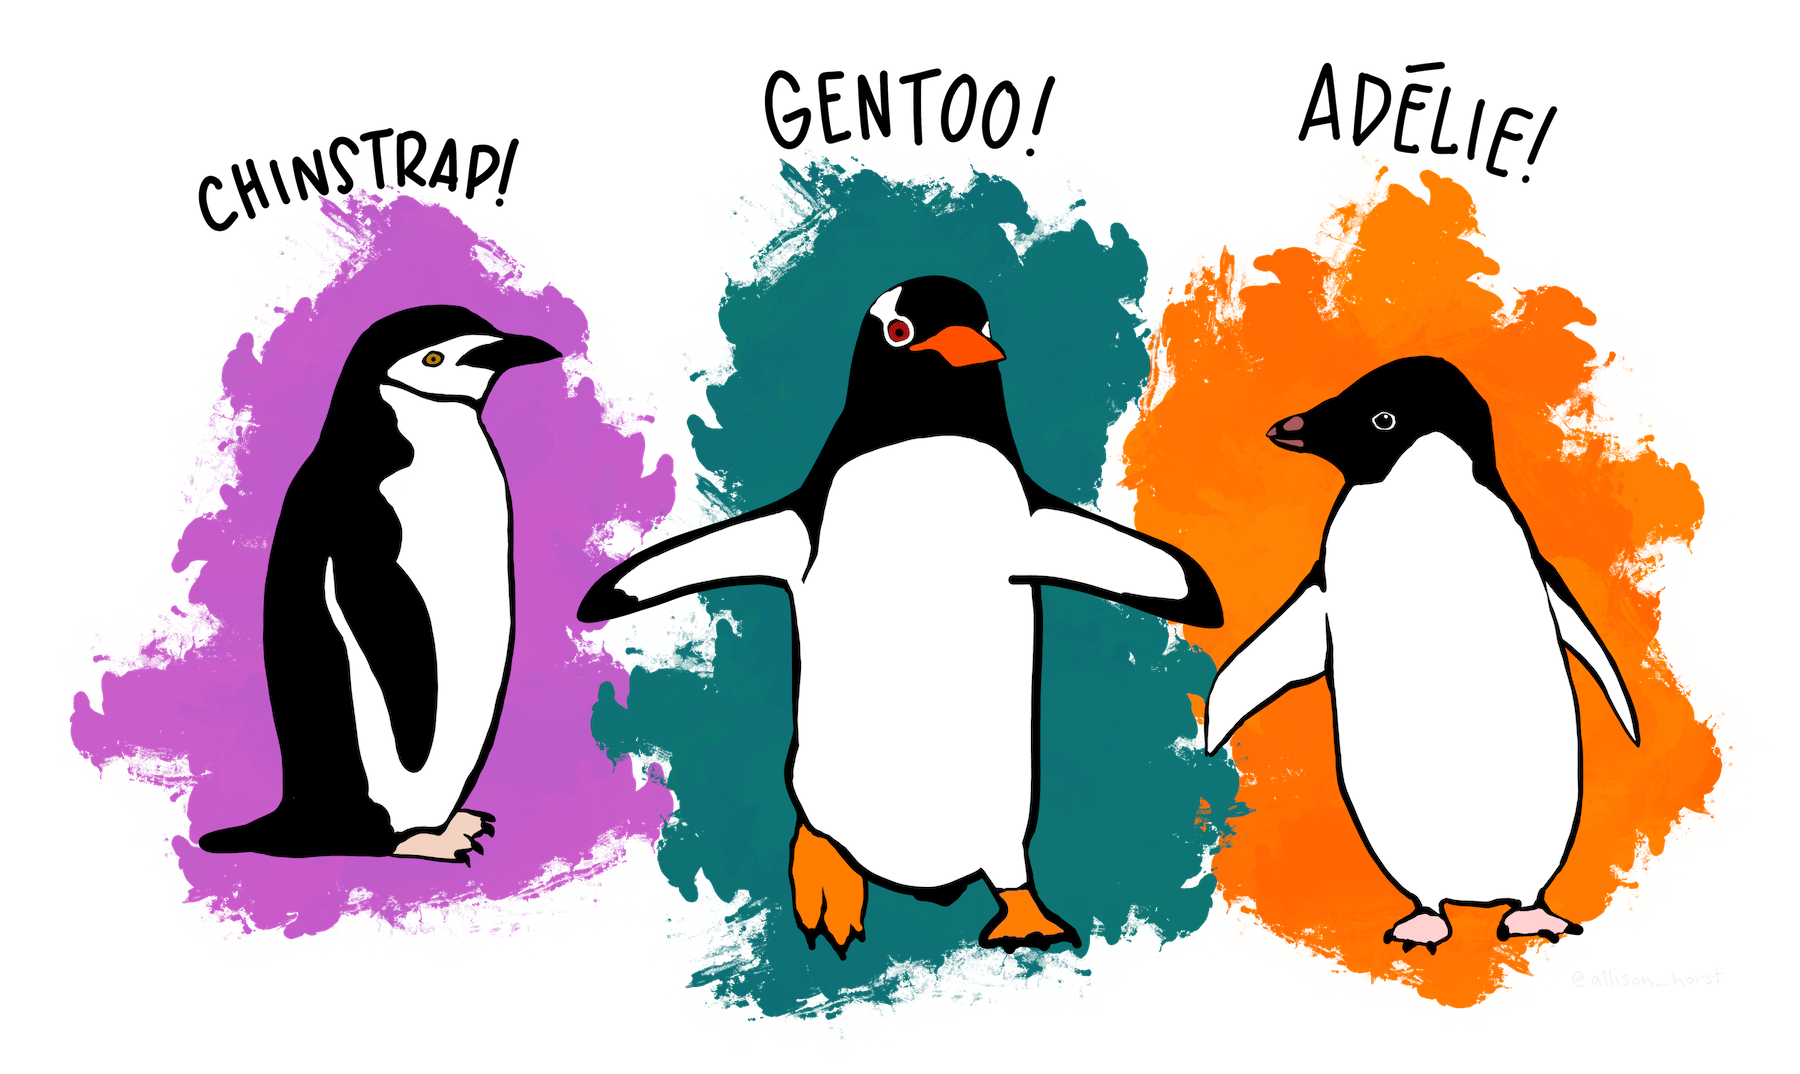
\includegraphics{./images/Penguins.png}

}

\caption{Les 3 espèces de manchots de l'archipel de Palmer. Illustration
: Allison Horst}

\end{figure}

\hypertarget{le-data-frame-penguins}{%
\section{\texorpdfstring{Le data frame
\texttt{penguins}}{Le data frame penguins}}\label{le-data-frame-penguins}}

Nous allons commencer par explorer le jeu de données \texttt{penguins}
qui est inclus avec le package \texttt{palmerpenguins} afin de nous
faire une idée de sa structure. Dans votre script, tapez la commande
suivante et exécutez la dans la console (selon les réglages de
\texttt{RStudio} et \emph{la largeur de votre console}, l'affichage peut
varier légèrement) :

\begin{Shaded}
\begin{Highlighting}[]
\NormalTok{penguins}
\end{Highlighting}
\end{Shaded}

\begin{verbatim}
# A tibble: 344 x 8
   species island    bill_length_mm bill_depth_mm flipper_~1 body_~2 sex    year
   <fct>   <fct>              <dbl>         <dbl>      <int>   <int> <fct> <int>
 1 Adelie  Torgersen           39.1          18.7        181    3750 male   2007
 2 Adelie  Torgersen           39.5          17.4        186    3800 fema~  2007
 3 Adelie  Torgersen           40.3          18          195    3250 fema~  2007
 4 Adelie  Torgersen           NA            NA           NA      NA <NA>   2007
 5 Adelie  Torgersen           36.7          19.3        193    3450 fema~  2007
 6 Adelie  Torgersen           39.3          20.6        190    3650 male   2007
 7 Adelie  Torgersen           38.9          17.8        181    3625 fema~  2007
 8 Adelie  Torgersen           39.2          19.6        195    4675 male   2007
 9 Adelie  Torgersen           34.1          18.1        193    3475 <NA>   2007
10 Adelie  Torgersen           42            20.2        190    4250 <NA>   2007
# ... with 334 more rows, and abbreviated variable names 1: flipper_length_mm,
#   2: body_mass_g
\end{verbatim}

Essayons de décrypter cet affichage :

\begin{itemize}
\tightlist
\item
  \texttt{A\ tibble:\ 344\ x\ 8} : un tibble est un \texttt{data.frame}
  amélioré. Il a toutes les caractéristiques d'un \texttt{data.frame},
  (tapez \texttt{class(penguins)} pour vous en convaincre), mais en
  plus, il a quelques propriétés intéressantes sur lesquelles nous
  reviendrons plus tard. Ce \texttt{tibble} possède donc :

  \begin{itemize}
  \tightlist
  \item
    344 lignes
  \item
    8 colonnes, qui correspondent aux variables. Dans un
    \texttt{tibble}, les observations sont toujours en lignes et les
    variables en colonnes
  \end{itemize}
\item
  \texttt{species}, \texttt{island}, \texttt{bill\_length\_mm},
  \texttt{bill\_depth\_mm}, \texttt{flipper\_length\_mm}\ldots{} sont
  les noms des colonnes, c'est à dire les variables de ce jeu de données
\item
  Nous avons ensuite les 10 premières lignes du tableau
\item
  \texttt{...\ with\ 334\ more\ rows,\ and\ abbreviated\ variable\ names...},
  nous indique que 334 lignes ne logent pas à l'écran et que le nom de
  certains variables a été abrégé afin de permettre un affichage plus
  clair. Ces données font toutefois partie intégrante du tableau
  \texttt{penguins}
\item
  les noms complets de toutes les variables abrégées sont également
  indiqués
\end{itemize}

Cette façon d'afficher les tableaux est spécifique des \texttt{tibble}s.
Vous noterez que le type de chaque variable est indiqué entre
\texttt{\textless{}...\textgreater{}}, juste sous les noms de colonnes.
Voici certains des types de données que vous pourrez rencontrer :

\begin{itemize}
\tightlist
\item
  \texttt{\textless{}int\textgreater{}} : nombres entiers (``integers'')
\item
  \texttt{\textless{}dbl\textgreater{}} : nombres réels (``doubles'')
\item
  \texttt{\textless{}chr\textgreater{}} : caractères (``characters'')
\item
  \texttt{\textless{}fct\textgreater{}} : facteurs (``factors'')
\item
  \texttt{\textless{}ord\textgreater{}} : facteurs ordonnés
  (``ordinals'')
\item
  \texttt{\textless{}lgl\textgreater{}} : logiques (colonne de
  vrais/faux : ``logical'')
\item
  \texttt{\textless{}date\textgreater{}} : dates
\item
  \texttt{\textless{}time\textgreater{}} : heures
\item
  \texttt{\textless{}dttm\textgreater{}} : combinaison de date et
  d'heure (``date time'')
\end{itemize}

Cette façon d'afficher le contenu d'un tableau permet d'y voir
(beaucoup) plus clair que l'affichage classique d'un
\texttt{data.frame}. Malheureusement, ce n'est pas toujours suffisant.
Voyons quelles sont les autres méthodes permettant d'explorer un
\texttt{data.frame}.

\hypertarget{explorer-un-data.frame}{%
\section{\texorpdfstring{Explorer un
\texttt{data.frame}}{Explorer un data.frame}}\label{explorer-un-data.frame}}

Parmi les nombreuses façons d'avoir une idée des données contenues dans
un \texttt{data.frame} tel que \texttt{penguins}, on présente ici 3
fonctions qui prennent le nom du \texttt{data.frame} en guise
d'argument, et un opérateur :

\begin{itemize}
\tightlist
\item
  la fonction \texttt{View()} intégrée à \texttt{RStudio}. C'est celle
  que vous utiliserez le plus souvent. Attention, elle s'écrit avec un
  ``V'' majuscule
\item
  la fonction \texttt{glimpse()} chargée avec le package \texttt{dplyr}.
  Elle est très similaire à la fonction \texttt{str()} découverte dans
  les tutoriels de DataCamp
\item
  l'opérateur \texttt{\$} permet d'accéder à une unique variable d'un
  \texttt{data.frame}
\item
  la fonction \texttt{skim()} du package \texttt{skimr} permet d'obtenir
  un résumé complet mais très synthétique et visuel des variables d'un
  \texttt{data.frame}
\end{itemize}

\hypertarget{sec-View}{%
\subsection{\texorpdfstring{\texttt{View()}}{View()}}\label{sec-View}}

Tapez \texttt{View(penguins)} dans votre script et exécutez la commande.
Un nouvel onglet contenant ce qui ressemble à un tableur doit s'ouvrir.

\begin{tcolorbox}[enhanced jigsaw, bottomtitle=1mm, title=\textcolor{quarto-callout-tip-color}{\faLightbulb}\hspace{0.5em}{Quizz : à quoi correspondent chacune des lignes de ce tableau ?}, breakable, opacitybacktitle=0.6, coltitle=black, opacityback=0, toprule=.15mm, toptitle=1mm, titlerule=0mm, colback=white, rightrule=.15mm, arc=.35mm, leftrule=.75mm, bottomrule=.15mm, left=2mm, colframe=quarto-callout-tip-color-frame, colbacktitle=quarto-callout-tip-color!10!white]

\begin{enumerate}
\def\labelenumi{\alph{enumi}.}
\tightlist
\item
  aux données d'une espèce
\item
  aux données d'une île
\item
  aux données d'un individu
\item
  aux données d'une population (plusieurs manchots à la fois)
\end{enumerate}

\end{tcolorbox}

Ici, vous pouvez donc explorer la totalité du tableau, passer chaque
variable en revue, et même appliquer des filtres pour ne visualiser
qu'une partie des données. Par exemple, essayez de déterminer combien
d'individus sont issus de l'île ``Biscoe''.

Ce tableau n'est pas facile à manipuler. Il est impossible de corriger
des valeurs, et lorsque l'on applique des filtres, il est impossible de
récupérer uniquement les données filtrées. Nous verrons plus tard
comment les obtenir en tapant des commandes simples dans un script. La
seule utilité de ce tableau est donc l'exploration visuelle des données.

\hypertarget{glimpse}{%
\subsection{\texorpdfstring{\texttt{glimpse()}}{glimpse()}}\label{glimpse}}

La seconde façon d'explorer les données contenues dans un tableau est
d'utiliser la fonction \texttt{glimpse()} après avoir chargé le package
\texttt{dplyr} :

\begin{Shaded}
\begin{Highlighting}[]
\FunctionTok{glimpse}\NormalTok{(penguins)}
\end{Highlighting}
\end{Shaded}

\begin{verbatim}
Rows: 344
Columns: 8
$ species           <fct> Adelie, Adelie, Adelie, Adelie, Adelie, Adelie, Adel~
$ island            <fct> Torgersen, Torgersen, Torgersen, Torgersen, Torgerse~
$ bill_length_mm    <dbl> 39.1, 39.5, 40.3, NA, 36.7, 39.3, 38.9, 39.2, 34.1, ~
$ bill_depth_mm     <dbl> 18.7, 17.4, 18.0, NA, 19.3, 20.6, 17.8, 19.6, 18.1, ~
$ flipper_length_mm <int> 181, 186, 195, NA, 193, 190, 181, 195, 193, 190, 186~
$ body_mass_g       <int> 3750, 3800, 3250, NA, 3450, 3650, 3625, 4675, 3475, ~
$ sex               <fct> male, female, female, NA, female, male, female, male~
$ year              <int> 2007, 2007, 2007, 2007, 2007, 2007, 2007, 2007, 2007~
\end{verbatim}

Ici, les premières observations sont présentées en lignes pour chaque
variable du jeu de données. Là encore, le type de chaque variable est
précisé. Essayez d'identifier 3 variables catégorielles. À quoi
correspondent-elles ? En quoi sont-elles différentes des variables
numériques ?

\hypertarget{lopuxe9rateur}{%
\subsection{\texorpdfstring{L'opérateur
\texttt{\$}}{L'opérateur \$}}\label{lopuxe9rateur}}

L'opérateur \texttt{\$} permet d'accéder à une unique variable grâce à
son nom. Par exemple on peut accéder à toutes les données concernant les
noms d'espèces (variable \texttt{species} du tableau \texttt{penguins})
en tapant :

\begin{Shaded}
\begin{Highlighting}[]
\NormalTok{penguins}\SpecialCharTok{$}\NormalTok{species}
\end{Highlighting}
\end{Shaded}

\begin{verbatim}
  [1] Adelie    Adelie    Adelie    Adelie    Adelie    Adelie    Adelie   
  [8] Adelie    Adelie    Adelie    Adelie    Adelie    Adelie    Adelie   
 [15] Adelie    Adelie    Adelie    Adelie    Adelie    Adelie    Adelie   
 [22] Adelie    Adelie    Adelie    Adelie    Adelie    Adelie    Adelie   
 [29] Adelie    Adelie    Adelie    Adelie    Adelie    Adelie    Adelie   
 [36] Adelie    Adelie    Adelie    Adelie    Adelie    Adelie    Adelie   
 [43] Adelie    Adelie    Adelie    Adelie    Adelie    Adelie    Adelie   
 [50] Adelie    Adelie    Adelie    Adelie    Adelie    Adelie    Adelie   
 [57] Adelie    Adelie    Adelie    Adelie    Adelie    Adelie    Adelie   
 [64] Adelie    Adelie    Adelie    Adelie    Adelie    Adelie    Adelie   
 [71] Adelie    Adelie    Adelie    Adelie    Adelie    Adelie    Adelie   
 [78] Adelie    Adelie    Adelie    Adelie    Adelie    Adelie    Adelie   
 [85] Adelie    Adelie    Adelie    Adelie    Adelie    Adelie    Adelie   
 [92] Adelie    Adelie    Adelie    Adelie    Adelie    Adelie    Adelie   
 [99] Adelie    Adelie    Adelie    Adelie    Adelie    Adelie    Adelie   
[106] Adelie    Adelie    Adelie    Adelie    Adelie    Adelie    Adelie   
[113] Adelie    Adelie    Adelie    Adelie    Adelie    Adelie    Adelie   
[120] Adelie    Adelie    Adelie    Adelie    Adelie    Adelie    Adelie   
[127] Adelie    Adelie    Adelie    Adelie    Adelie    Adelie    Adelie   
[134] Adelie    Adelie    Adelie    Adelie    Adelie    Adelie    Adelie   
[141] Adelie    Adelie    Adelie    Adelie    Adelie    Adelie    Adelie   
[148] Adelie    Adelie    Adelie    Adelie    Adelie    Gentoo    Gentoo   
[155] Gentoo    Gentoo    Gentoo    Gentoo    Gentoo    Gentoo    Gentoo   
[162] Gentoo    Gentoo    Gentoo    Gentoo    Gentoo    Gentoo    Gentoo   
[169] Gentoo    Gentoo    Gentoo    Gentoo    Gentoo    Gentoo    Gentoo   
[176] Gentoo    Gentoo    Gentoo    Gentoo    Gentoo    Gentoo    Gentoo   
[183] Gentoo    Gentoo    Gentoo    Gentoo    Gentoo    Gentoo    Gentoo   
[190] Gentoo    Gentoo    Gentoo    Gentoo    Gentoo    Gentoo    Gentoo   
[197] Gentoo    Gentoo    Gentoo    Gentoo    Gentoo    Gentoo    Gentoo   
[204] Gentoo    Gentoo    Gentoo    Gentoo    Gentoo    Gentoo    Gentoo   
[211] Gentoo    Gentoo    Gentoo    Gentoo    Gentoo    Gentoo    Gentoo   
[218] Gentoo    Gentoo    Gentoo    Gentoo    Gentoo    Gentoo    Gentoo   
[225] Gentoo    Gentoo    Gentoo    Gentoo    Gentoo    Gentoo    Gentoo   
[232] Gentoo    Gentoo    Gentoo    Gentoo    Gentoo    Gentoo    Gentoo   
[239] Gentoo    Gentoo    Gentoo    Gentoo    Gentoo    Gentoo    Gentoo   
[246] Gentoo    Gentoo    Gentoo    Gentoo    Gentoo    Gentoo    Gentoo   
[253] Gentoo    Gentoo    Gentoo    Gentoo    Gentoo    Gentoo    Gentoo   
[260] Gentoo    Gentoo    Gentoo    Gentoo    Gentoo    Gentoo    Gentoo   
[267] Gentoo    Gentoo    Gentoo    Gentoo    Gentoo    Gentoo    Gentoo   
[274] Gentoo    Gentoo    Gentoo    Chinstrap Chinstrap Chinstrap Chinstrap
[281] Chinstrap Chinstrap Chinstrap Chinstrap Chinstrap Chinstrap Chinstrap
[288] Chinstrap Chinstrap Chinstrap Chinstrap Chinstrap Chinstrap Chinstrap
[295] Chinstrap Chinstrap Chinstrap Chinstrap Chinstrap Chinstrap Chinstrap
[302] Chinstrap Chinstrap Chinstrap Chinstrap Chinstrap Chinstrap Chinstrap
[309] Chinstrap Chinstrap Chinstrap Chinstrap Chinstrap Chinstrap Chinstrap
[316] Chinstrap Chinstrap Chinstrap Chinstrap Chinstrap Chinstrap Chinstrap
[323] Chinstrap Chinstrap Chinstrap Chinstrap Chinstrap Chinstrap Chinstrap
[330] Chinstrap Chinstrap Chinstrap Chinstrap Chinstrap Chinstrap Chinstrap
[337] Chinstrap Chinstrap Chinstrap Chinstrap Chinstrap Chinstrap Chinstrap
[344] Chinstrap
Levels: Adelie Chinstrap Gentoo
\end{verbatim}

Cela nous permet de récupérer les données sous la forme d'un vecteur.
Attention toutefois, le tableau \texttt{penguins} contient beaucoup de
lignes. Récupérer une variable grâce à cet opérateur peut rapidement
saturer la console. Nous serons amenés à manipuler des tableaux
contenant plusieurs dizaines ou centaines de milliers de lignes. C'est
le cas du tableau \texttt{diamonds} du package \texttt{ggplot2} que vous
avez découvert dans les exercice de la Section~\ref{sec-Exo-1}.

Si, par exemple, vous souhaitez extraire les données relatives à la
clarté des diamants (colonne \texttt{clarity}) du tableau
\texttt{diamonds}, vous pouvez taper ceci :

\begin{Shaded}
\begin{Highlighting}[]
\FunctionTok{library}\NormalTok{(ggplot2)}
\NormalTok{diamonds}\SpecialCharTok{$}\NormalTok{clarity}
\end{Highlighting}
\end{Shaded}

Le résultat est pour le moins indigeste ! Lorsqu'un tableau contient de
nombreuses lignes, c'est rarement une bonne idée de transformer l'une de
ses colonnes en vecteur. Dans la mesure du possible, les données d'un
tableau doivent rester dans le tableau.

\hypertarget{skim}{%
\subsection{\texorpdfstring{\texttt{skim()}}{skim()}}\label{skim}}

Pour utiliser la fonction \texttt{skim()}, vous devez au préalable
installer le package \texttt{skimr} :

\begin{Shaded}
\begin{Highlighting}[]
\FunctionTok{install.packages}\NormalTok{(}\StringTok{"skimr"}\NormalTok{)}
\end{Highlighting}
\end{Shaded}

Ce package est un peu ``expérimental'' et il se peut que l'installation
pose problème. Si un message d'erreur apparaît lors de l'installation,
procédez comme suit :

\begin{enumerate}
\def\labelenumi{\arabic{enumi}.}
\tightlist
\item
  Quittez \texttt{RStudio} (sans oublier de sauvegarder votre travail au
  préalable)
\item
  Relancez \texttt{RStudio} et dans la console, tapez ceci :
\end{enumerate}

\begin{Shaded}
\begin{Highlighting}[]
\FunctionTok{install.packages}\NormalTok{(}\StringTok{"rlang"}\NormalTok{)}
\end{Highlighting}
\end{Shaded}

\begin{enumerate}
\def\labelenumi{\arabic{enumi}.}
\setcounter{enumi}{2}
\tightlist
\item
  Tentez d'installer \texttt{skimr} à nouveau.
\item
  Exécutez à nouveau tout votre script afin de retrouver votre travail
  dans l'état où il était avant de quitter \texttt{RStudio}.
\end{enumerate}

Si l'installation de \texttt{skimr} s'est bien passée, vous pouvez
maintenant taper ceci :

\begin{Shaded}
\begin{Highlighting}[]
\FunctionTok{library}\NormalTok{(skimr)}
\FunctionTok{skim}\NormalTok{(penguins)}
\end{Highlighting}
\end{Shaded}

\begin{longtable}[]{@{}ll@{}}
\caption{Data summary}\tabularnewline
\toprule()
\endhead
Name & penguins \\
Number of rows & 344 \\
Number of columns & 8 \\
\_\_\_\_\_\_\_\_\_\_\_\_\_\_\_\_\_\_\_\_\_\_\_ & \\
Column type frequency: & \\
factor & 3 \\
numeric & 5 \\
\_\_\_\_\_\_\_\_\_\_\_\_\_\_\_\_\_\_\_\_\_\_\_\_ & \\
Group variables & None \\
\bottomrule()
\end{longtable}

\textbf{Variable type: factor}

\begin{longtable}[]{@{}
  >{\raggedright\arraybackslash}p{(\columnwidth - 10\tabcolsep) * \real{0.1687}}
  >{\raggedleft\arraybackslash}p{(\columnwidth - 10\tabcolsep) * \real{0.1205}}
  >{\raggedleft\arraybackslash}p{(\columnwidth - 10\tabcolsep) * \real{0.1687}}
  >{\raggedright\arraybackslash}p{(\columnwidth - 10\tabcolsep) * \real{0.0964}}
  >{\raggedleft\arraybackslash}p{(\columnwidth - 10\tabcolsep) * \real{0.1084}}
  >{\raggedright\arraybackslash}p{(\columnwidth - 10\tabcolsep) * \real{0.3373}}@{}}
\toprule()
\begin{minipage}[b]{\linewidth}\raggedright
skim\_variable
\end{minipage} & \begin{minipage}[b]{\linewidth}\raggedleft
n\_missing
\end{minipage} & \begin{minipage}[b]{\linewidth}\raggedleft
complete\_rate
\end{minipage} & \begin{minipage}[b]{\linewidth}\raggedright
ordered
\end{minipage} & \begin{minipage}[b]{\linewidth}\raggedleft
n\_unique
\end{minipage} & \begin{minipage}[b]{\linewidth}\raggedright
top\_counts
\end{minipage} \\
\midrule()
\endhead
species & 0 & 1.00 & FALSE & 3 & Ade: 152, Gen: 124, Chi: 68 \\
island & 0 & 1.00 & FALSE & 3 & Bis: 168, Dre: 124, Tor: 52 \\
sex & 11 & 0.97 & FALSE & 2 & mal: 168, fem: 165 \\
\bottomrule()
\end{longtable}

\textbf{Variable type: numeric}

\begin{longtable}[]{@{}
  >{\raggedright\arraybackslash}p{(\columnwidth - 20\tabcolsep) * \real{0.1800}}
  >{\raggedleft\arraybackslash}p{(\columnwidth - 20\tabcolsep) * \real{0.1000}}
  >{\raggedleft\arraybackslash}p{(\columnwidth - 20\tabcolsep) * \real{0.1400}}
  >{\raggedleft\arraybackslash}p{(\columnwidth - 20\tabcolsep) * \real{0.0800}}
  >{\raggedleft\arraybackslash}p{(\columnwidth - 20\tabcolsep) * \real{0.0700}}
  >{\raggedleft\arraybackslash}p{(\columnwidth - 20\tabcolsep) * \real{0.0700}}
  >{\raggedleft\arraybackslash}p{(\columnwidth - 20\tabcolsep) * \real{0.0800}}
  >{\raggedleft\arraybackslash}p{(\columnwidth - 20\tabcolsep) * \real{0.0800}}
  >{\raggedleft\arraybackslash}p{(\columnwidth - 20\tabcolsep) * \real{0.0700}}
  >{\raggedleft\arraybackslash}p{(\columnwidth - 20\tabcolsep) * \real{0.0700}}
  >{\raggedright\arraybackslash}p{(\columnwidth - 20\tabcolsep) * \real{0.0600}}@{}}
\toprule()
\begin{minipage}[b]{\linewidth}\raggedright
skim\_variable
\end{minipage} & \begin{minipage}[b]{\linewidth}\raggedleft
n\_missing
\end{minipage} & \begin{minipage}[b]{\linewidth}\raggedleft
complete\_rate
\end{minipage} & \begin{minipage}[b]{\linewidth}\raggedleft
mean
\end{minipage} & \begin{minipage}[b]{\linewidth}\raggedleft
sd
\end{minipage} & \begin{minipage}[b]{\linewidth}\raggedleft
p0
\end{minipage} & \begin{minipage}[b]{\linewidth}\raggedleft
p25
\end{minipage} & \begin{minipage}[b]{\linewidth}\raggedleft
p50
\end{minipage} & \begin{minipage}[b]{\linewidth}\raggedleft
p75
\end{minipage} & \begin{minipage}[b]{\linewidth}\raggedleft
p100
\end{minipage} & \begin{minipage}[b]{\linewidth}\raggedright
hist
\end{minipage} \\
\midrule()
\endhead
bill\_length\_mm & 2 & 0.99 & 43.92 & 5.46 & 32.1 & 39.23 & 44.45 & 48.5
& 59.6 & ▃▇▇▆▁ \\
bill\_depth\_mm & 2 & 0.99 & 17.15 & 1.97 & 13.1 & 15.60 & 17.30 & 18.7
& 21.5 & ▅▅▇▇▂ \\
flipper\_length\_mm & 2 & 0.99 & 200.92 & 14.06 & 172.0 & 190.00 &
197.00 & 213.0 & 231.0 & ▂▇▃▅▂ \\
body\_mass\_g & 2 & 0.99 & 4201.75 & 801.95 & 2700.0 & 3550.00 & 4050.00
& 4750.0 & 6300.0 & ▃▇▆▃▂ \\
year & 0 & 1.00 & 2008.03 & 0.82 & 2007.0 & 2007.00 & 2008.00 & 2009.0 &
2009.0 & ▇▁▇▁▇ \\
\bottomrule()
\end{longtable}

Nous aurons l'occasion de revenir en détail sur la signification de tous
ces indices au semestre prochain. À ce stade, retenez que cette fonction
\texttt{skim()} permet d'accéder à un résumé très détaillé de chaque
variable d'un jeu de données. Par exemple, on apprend ici que la masse
corporelle moyenne des manchots de l'ensemble du jeu de données vaut
4201.75 grammes (ligne \texttt{body\_mass\_g}, colonne \texttt{mean}),
avec un écart-type de 0.82 grammes (colonne \texttt{sd}), et que la
masse de 2 individus est manquante (colonne \texttt{n\_missing}). Cette
fonction nous sera donc très utile au semestre prochain lorsque nous
aborderons la question des statistiques descriptives.

\hypertarget{les-fichiers-daide}{%
\subsection{Les fichiers d'aide}\label{les-fichiers-daide}}

Une fonctionnalité particulièrement utile de \texttt{R} est son système
d'aide. On peut obtenir de l'aide au sujet de n'importe quelle fonction
et de n'importe quel jeu de données en tapant un ``\texttt{?}''
immédiatement suivi du nom de la fonction ou de l'objet.

Par exemple, examinez l'aide du jeu de données \texttt{penguins} :

\begin{Shaded}
\begin{Highlighting}[]
\NormalTok{?penguins}
\end{Highlighting}
\end{Shaded}

Vous devriez absolument prendre l'habitude d'examiner les fichiers
d'aide des fonctions ou jeux de données pour lesquels vous avez des
questions. Ces fichiers sont très complets, et même s'il peuvent
paraître impressionnants au premier abord, ils sont tous structurés sur
le même modèle et vous aideront à comprendre comment utiliser les
fonctions, quels sont les arguments possibles, à quoi ils servent et
comment les utiliser.

Prenez le temps d'examiner le fichier d'aide du jeu de données
\texttt{penguins}. Avant de passer à la suite, assurez-vous d'avoir
compris à quoi correspondent chacune des 8 variables de ce tableau.

\hypertarget{sec-Exo-2}{%
\section{Exercices}\label{sec-Exo-2}}

Consultez l'aide du jeu de données \texttt{diamonds} du package
\texttt{ggplot2}.

\begin{itemize}
\tightlist
\item
  Quel est le code de la couleur la plus prisée ?
\item
  Quel est le code de la moins bonne clarté ?
\item
  À quoi correspond la variable \texttt{z} ?
\item
  En quoi la variable \texttt{depth} est-elle différente de la variable
  \texttt{z} ?
\end{itemize}

\bookmarksetup{startatroot}

\hypertarget{sec-viz}{%
\chapter{\texorpdfstring{Visualiser des données avec
\texttt{ggplot2}}{Visualiser des données avec ggplot2}}\label{sec-viz}}

\hypertarget{pruxe9ambule-2}{%
\section{Préambule}\label{pruxe9ambule-2}}

Dans le Chapitre~\ref{sec-bases} et le Chapitre~\ref{sec-dataset}, vous
avez découvert les concepts essentiels qu'il est important de maîtriser
avant de commencer à explorer en détail des données dans \texttt{R}. Les
éléments de syntaxe abordés dans la Section~\ref{sec-code} sont nombreux
et vous n'avez probablement pas tout retenu. C'est pourquoi je vous
conseille de garder les tutoriels de DataCamp à portée de main afin de
pouvoir refaire les parties que vous maîtrisez le moins. Ce n'est qu'en
répétant plusieurs fois ces tutoriels que les choses seront vraiment
comprises et que vous les retiendrez. Ainsi, si des éléments de code
présentés ci-dessous vous semblent obscurs, revenez en arrière : toutes
les réponses à vos questions se trouvent probablement dans les chapitres
précédents.

Après la découverte des bases du langage \texttt{R}, nous abordons
maintenant les parties de ce livre qui concernent la ``science des
données'' (ou ``Data Science'' pour nos amis anglo-saxons). Nous allons
voir dans ce chapitre qu'outre les fonctions \texttt{View()} et
\texttt{glimpse()}, l'exploration visuelle \emph{via} la représentation
graphique des données est un moyen indispensable et très puissant pour
comprendre ce qui se passe dans un jeu de données.

\begin{tcolorbox}[enhanced jigsaw, bottomtitle=1mm, title=\textcolor{quarto-callout-important-color}{\faExclamation}\hspace{0.5em}{Important}, breakable, opacitybacktitle=0.6, coltitle=black, opacityback=0, toprule=.15mm, toptitle=1mm, titlerule=0mm, colback=white, rightrule=.15mm, arc=.35mm, leftrule=.75mm, bottomrule=.15mm, left=2mm, colframe=quarto-callout-important-color-frame, colbacktitle=quarto-callout-important-color!10!white]
La visualisation de vos données devrait toujours être un
\textbf{préalable indispensable} à toute analyse statistique.
\end{tcolorbox}

La visualisation des données est en outre un excellent point de départ
quand on découvre la programmation sous \texttt{R}, car ses bénéfices
sont clairs et immédiats : vous pouvez créer des graphiques élégants et
informatifs qui vous aident à comprendre les données. Dans ce chapitre,
vous allez donc plonger dans l'art de la visualisation des données, en
apprenant la structure de base des graphiques réalisés avec
\texttt{ggplot2} qui permettent de transformer des données numériques et
catégorielles en graphiques.

Toutefois, la visualisation seule ne suffit généralement pas. Il est en
effet souvent nécessaire de transformer les données pour produire des
représentations plus parlantes. Ainsi, dans le
Chapitre~\ref{sec-wrangling}, vous découvrirez les fonctions clés qui
vous permettront de sélectionner des variables importantes, de filtrer
des observations, de créer de nouvelles variables, ou d'en modifier la
forme.

Ce n'est qu'en combinant les transformations de données et
représentations graphiques d'une part, avec votre curiosité et votre
esprit critique d'autre part, que vous serez véritablement en mesure de
réaliser une analyse exploratoire de vos données à la fois utile et
pertinente. C'est la seule façon d'identifier des questions
intéressantes sur vos données, afin de tenter d'y répondre par les
analyses statistiques et la modélisation qui seront abordées lors des
prochains semestres.

\begin{center}\rule{0.5\linewidth}{0.5pt}\end{center}

Dans ce chapitre, nous aurons besoin des packages suivants :

\begin{Shaded}
\begin{Highlighting}[]
\FunctionTok{library}\NormalTok{(ggplot2)}
\FunctionTok{library}\NormalTok{(dplyr)}
\FunctionTok{library}\NormalTok{(palmerpenguins)}
\end{Highlighting}
\end{Shaded}

Si ce n'est pas déjà fait, pensez à les installer avant de les charger
en mémoire.

Au niveau le plus élémentaire, les graphiques permettent de comprendre
comment les variables se comparent en termes de tendance centrale (à
quel endroit les valeurs ont tendance à être localisées, regroupées) et
leur dispersion (comment les données varient autour du centre). La chose
la plus importante à savoir sur les graphiques est qu'ils doivent être
créés pour que votre public (le professeur qui vous évalue, le collègue
avec qui vous collaborez, votre futur employeur, etc.) comprenne bien
les résultats et les informations que vous souhaitez transmettre. Il
s'agit d'un exercice d'équilibriste : d'une part, vous voulez mettre en
évidence autant de relations significatives et de résultats intéressants
que possible, mais de l'autre, vous ne voulez pas trop en inclure, afin
d'éviter de rendre votre graphique illisible ou de submerger votre
public. Tout comme n'importe quel paragraphe de document écrit, un
graphique doit permettre de \textbf{communiquer un message} (une idée
forte, un résultat marquant, une hypothèse nouvelle, etc).

Comme nous le verrons, les graphiques nous aident également à repérer
les tendances extrêmes et les valeurs aberrantes dans nos données. Nous
verrons aussi qu'une façon de faire, assez classique, consiste à
comparer la distribution d'une variable quantitative pour les différents
niveaux d'une variable catégorielle.

\begin{tcolorbox}[enhanced jigsaw, bottomtitle=1mm, title=\textcolor{quarto-callout-tip-color}{\faLightbulb}\hspace{0.5em}{Objectifs}, breakable, opacitybacktitle=0.6, coltitle=black, opacityback=0, toprule=.15mm, toptitle=1mm, titlerule=0mm, colback=white, rightrule=.15mm, arc=.35mm, leftrule=.75mm, bottomrule=.15mm, left=2mm, colframe=quarto-callout-tip-color-frame, colbacktitle=quarto-callout-tip-color!10!white]

Dans ce chapitre, vous apprendrez à :

\begin{enumerate}
\def\labelenumi{\arabic{enumi}.}
\tightlist
\item
  faire différents types de graphiques exploratoires avec le package
  \texttt{ggplot2} \faIcon{chart-line} \faIcon{chart-gantt}
  \faIcon{chart-column} \faIcon{chart-area}
\item
  choisir le ou les graphiques appropriés selon la nature des variables
  dont vous disposez ou que vous souhaitez mettre en relation
\item
  mettre vos graphiques en forme pour les intégrer dans vos rapports ou
  compte-rendus de TP
\end{enumerate}

\end{tcolorbox}

\hypertarget{sec-gggraph}{%
\section{La grammaire des graphiques}\label{sec-gggraph}}

Les lettres \texttt{gg} du package \texttt{ggplot2} sont l'abréviation
de ``\textbf{g}rammar of \textbf{g}raphics'' : la grammaire des
graphiques. De la même manière que nous construisons des phrases en
respectant des règles grammaticales précises (usage des noms, des
verbes, des sujets et adjectifs\ldots), la grammaire des graphiques
établit un certain nombre de règles permettant de construire des
graphiques : elle précise les composants d'un graphique en suivant le
cadre théorique défini par Wilkinson (2005).

\hypertarget{uxe9luxe9ments-de-la-grammaire}{%
\subsection{Éléments de la
grammaire}\label{uxe9luxe9ments-de-la-grammaire}}

En bref, la grammaire des graphiques nous dit que :

\begin{quote}
Un graphique est l'association (\texttt{mapping}) de données/variables
(\texttt{data}) à des attributs esthétiques (\texttt{aes}thetics)
d'objets géométriques (\texttt{geom}etric objects).
\end{quote}

Pour clarifier, on peut disséquer un graphique en 3 éléments essentiels
:

\begin{enumerate}
\def\labelenumi{\arabic{enumi}.}
\tightlist
\item
  \texttt{data} : le jeu de données contenant les variables que l'on va
  associer à des objets géométriques. Pour \texttt{ggplot2} les données
  doivent obligatoirement être stockées dans un \texttt{data.frame} ou
  un \texttt{tibble}
\item
  \texttt{geom} : les objets géométriques en question. Cela fait
  référence aux types d'objets que l'on peut observer sur le graphique
  (des points, des lignes, des barres, etc.)
\item
  \texttt{aes} : les attributs esthétiques des objets géométriques
  présents sur le graphique. Par exemple, la position sur les axes
  \texttt{x} et \texttt{y}, la couleur, la taille, la transparence, la
  forme, etc. Chacun de ces attributs esthétiques peut-être associé à
  une variable de notre jeu de données.
\end{enumerate}

Examinons un exemple pour bien comprendre.

\hypertarget{gapminder}{%
\subsection{Gapminder}\label{gapminder}}

En février 2006, un statisticien du nom de Hans Rosling a donné un TED
Talk intitulé
``\href{https://www.ted.com/talks/hans_rosling_shows_the_best_stats_you_ve_ever_seen}{The
best stats you'we ever seen}''. Au cours de cette conférence, Hans
Rosling présente des données sur l'économie mondiale, la santé et le
développement des pays du monde. Les données sont disponibles
\href{https://www.gapminder.org/tools/\#$chart-type=bubbles}{sur ce
site} et dans
\href{https://cran.r-project.org/web/packages/gapminder/index.html}{le
package \texttt{gapminder}}.

Pour l'année 2007, le jeu de données contient des informations pour 142
pays. Examinons les premières lignes de ce jeu de données :

\begin{longtable}[]{@{}llrrr@{}}
\caption{Les 6 premières lignes du jeu de données \texttt{gapminder}
pour l'année 2007.}\tabularnewline
\toprule()
Country & Continent & Life Expectancy & Population & GDP per Capita \\
\midrule()
\endfirsthead
\toprule()
Country & Continent & Life Expectancy & Population & GDP per Capita \\
\midrule()
\endhead
Afghanistan & Asia & 43.828 & 31889923 & 974.5803 \\
Albania & Europe & 76.423 & 3600523 & 5937.0295 \\
Algeria & Africa & 72.301 & 33333216 & 6223.3675 \\
Angola & Africa & 42.731 & 12420476 & 4797.2313 \\
Argentina & Americas & 75.320 & 40301927 & 12779.3796 \\
Australia & Oceania & 81.235 & 20434176 & 34435.3674 \\
\bottomrule()
\end{longtable}

Pour chaque ligne, les variables suivantes sont décrites :

\begin{itemize}
\tightlist
\item
  \texttt{Country} : le pays
\item
  \texttt{Continent} : le continent
\item
  \texttt{Life\ Expectancy} : espérance de vie à la naissance
\item
  \texttt{Population} : nombre de personnes vivant dans le pays
\item
  \texttt{GDP\ per\ Capita} : produit intérieur brut (PIB) par habitant
  en dollars américains. GDP est l'abréviation de ``Growth Domestic
  Product''. C'est un indicateur de l'activité économique d'un pays,
  parfois utilisé comme une approximation du revenu moyen par habitant.
\end{itemize}

Examinons maintenant la Figure~\ref{fig-gapminder} qui représente ces
variables pour chacun des 142 pays de ce jeu de données (notez
l'utilisation de la notation scientifique dans la légende, et de
l'échelle logarithmique de l'axe des abscisses).

\begin{figure}

{\centering 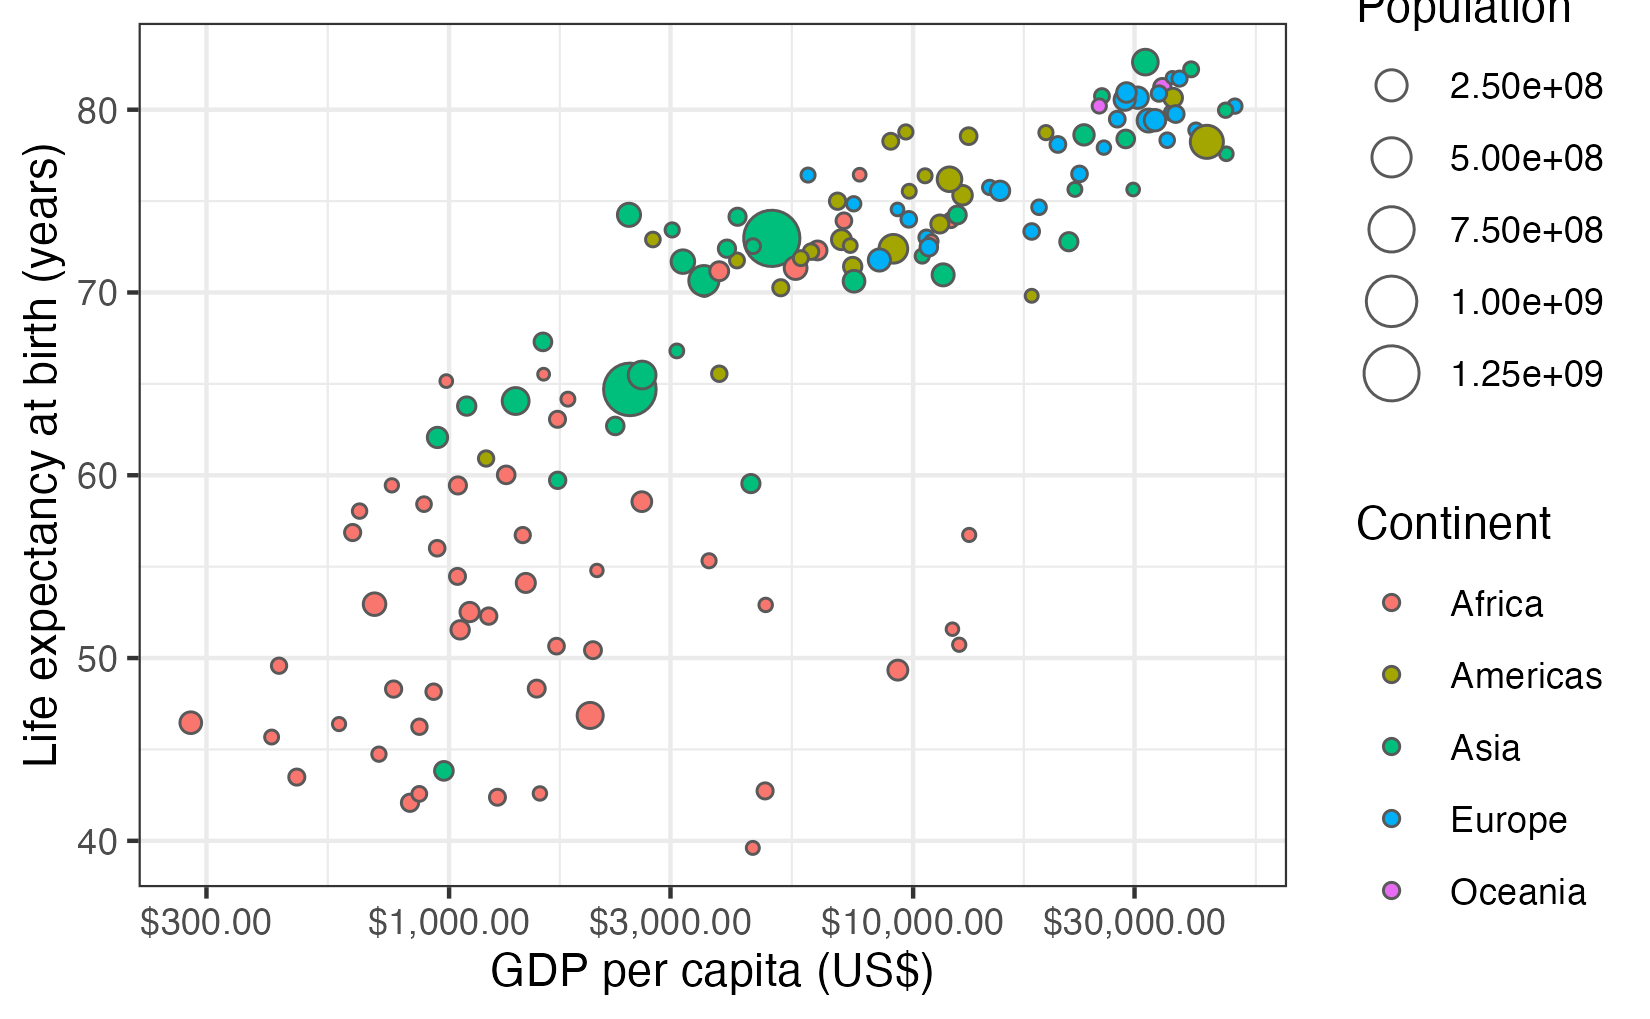
\includegraphics{./03-visualization_files/figure-pdf/fig-gapminder-1.png}

}

\caption{\label{fig-gapminder}Espérance de vie en fonction du PIB par
habitant en 2007.}

\end{figure}

Si on décrypte ce graphique du point de vue de la grammaire des
graphiques, on voit que :

\begin{itemize}
\tightlist
\item
  la variable \texttt{GDP\ per\ Capita} est associée à
  l'\texttt{aes}thetic \texttt{x} de la position des points
\item
  la variable \texttt{Life\ Expectancy} est associée à
  l'\texttt{aes}thetic \texttt{y} de la position des points
\item
  la variable \texttt{Population} est associée à l'\texttt{aes}thetic
  \texttt{size} (taille) des points
\item
  la variable \texttt{Continent} est associée à l'\texttt{aes}thetic
  \texttt{color} (couleur) des points
\end{itemize}

Ici, l'objet géométrique (ou \texttt{geom}) qui représente les données
est le point. Les données (ou \texttt{data}) sont contenues dans le
tableau \texttt{gapminder} et chacune de ces variables est associée
(\texttt{mapping}) aux caractéristiques esthétiques des points.

\hypertarget{autres-uxe9luxe9ments-de-la-grammaire-des-graphiques}{%
\subsection{Autres éléments de la grammaire des
graphiques}\label{autres-uxe9luxe9ments-de-la-grammaire-des-graphiques}}

Outre les éléments indispensables évoqués ici (\texttt{data},
\texttt{mapping}, \texttt{aes}, et \texttt{geom}), il existe d'autres
aspects de la grammaire des graphiques qui permettent de contrôler
l'aspect des graphiques. Ils ne sont pas toujours indispensables. Nous
en verrons néanmoins quelque-uns particulièrement utiles :

\begin{itemize}
\tightlist
\item
  \texttt{facet} : c'est un moyen très pratique de scinder le jeu de
  données en plusieurs sous-groupes et de produire automatiquement un
  graphique pour chacun d'entre eux.
\item
  \texttt{position} : permet notamment de modifier la position des
  barres d'un barplot.
\item
  \texttt{labs} : permet de définir les titres, sous-titres et légendes
  des axes d'un graphique
\item
  \texttt{theme} : permet de modifier l'apect général des graphiques en
  appliquant des thèmes prédéfinis ou en modifiant certains aspects de
  thèmes existants
\end{itemize}

\hypertarget{le-package-ggplot2}{%
\subsection{\texorpdfstring{Le package
\texttt{ggplot2}}{Le package ggplot2}}\label{le-package-ggplot2}}

Comme indiqué plus haut, le package \texttt{ggplot2} (Wickham et al.
2022) permet de réaliser des graphiques dans \texttt{R} en respectant
les principes de la grammaire des graphiques. Vous avez probablement
remarqué que depuis le début de la section Section~\ref{sec-gggraph},
beaucoup de termes sont écrits dans la police réservée au \texttt{code}
informatique. C'est parce que les éléments de la grammaire des
graphiques sont tous précisés dans la fonction \texttt{ggplot()} qui
demande, au grand minimum, que les éléments suivants soient spécifiés :

\begin{itemize}
\tightlist
\item
  le nom du \texttt{data.frame} contenant les variables qui seront
  utilisées pour le graphique. Ce nom correspond à l'argument
  \texttt{data} de la fonction \texttt{ggplot()}.
\item
  l'association des variables à des attributs esthétiques. Cela se fait
  grâce à l'argument \texttt{mapping} et la fonction \texttt{aes()}
\end{itemize}

Après avoir spécifié ces éléments, on ajoute des couches supplémentaires
au graphique grâce au signe \texttt{+}. La couche la plus essentielle à
ajouter à un graphique, est une couche contenant un élément géométrique,
ou \texttt{geom} (par exemple des points, des lignes ou des barres).
D'autres couches peuvent s'ajouter pour spécifier des titres, des
\texttt{facet}s ou des modifications des axes et des thèmes du
graphique.

Dans le cadre de ce cours, nous nous limiterons aux 5 types de
graphiques suivants :

\begin{enumerate}
\def\labelenumi{\arabic{enumi}.}
\tightlist
\item
  les nuages de points
\item
  les graphiques en lignes
\item
  les histogrammes
\item
  les diagrammes bâtons
\item
  les boîtes à moustaches (mais nous en dirons plus à ce sujet au
  semestre prochain)
\end{enumerate}

\hypertarget{votre-premier-graphique}{%
\subsection{Votre premier graphique}\label{votre-premier-graphique}}

Reprenons maintenant le jeu de données \texttt{penguins} :

\begin{Shaded}
\begin{Highlighting}[]
\NormalTok{penguins}
\end{Highlighting}
\end{Shaded}

\begin{verbatim}
# A tibble: 344 x 8
   species island    bill_length_mm bill_depth_mm flipper_~1 body_~2 sex    year
   <fct>   <fct>              <dbl>         <dbl>      <int>   <int> <fct> <int>
 1 Adelie  Torgersen           39.1          18.7        181    3750 male   2007
 2 Adelie  Torgersen           39.5          17.4        186    3800 fema~  2007
 3 Adelie  Torgersen           40.3          18          195    3250 fema~  2007
 4 Adelie  Torgersen           NA            NA           NA      NA <NA>   2007
 5 Adelie  Torgersen           36.7          19.3        193    3450 fema~  2007
 6 Adelie  Torgersen           39.3          20.6        190    3650 male   2007
 7 Adelie  Torgersen           38.9          17.8        181    3625 fema~  2007
 8 Adelie  Torgersen           39.2          19.6        195    4675 male   2007
 9 Adelie  Torgersen           34.1          18.1        193    3475 <NA>   2007
10 Adelie  Torgersen           42            20.2        190    4250 <NA>   2007
# ... with 334 more rows, and abbreviated variable names 1: flipper_length_mm,
#   2: body_mass_g
\end{verbatim}

Comme évoqué plus haut, il s'agit d'un \texttt{tibble}. Plusieurs de ses
variables concernent la biométrie des manchots, en particulier de son
bec (voir Figure~\ref{fig-morpho}).

\begin{figure}

{\centering 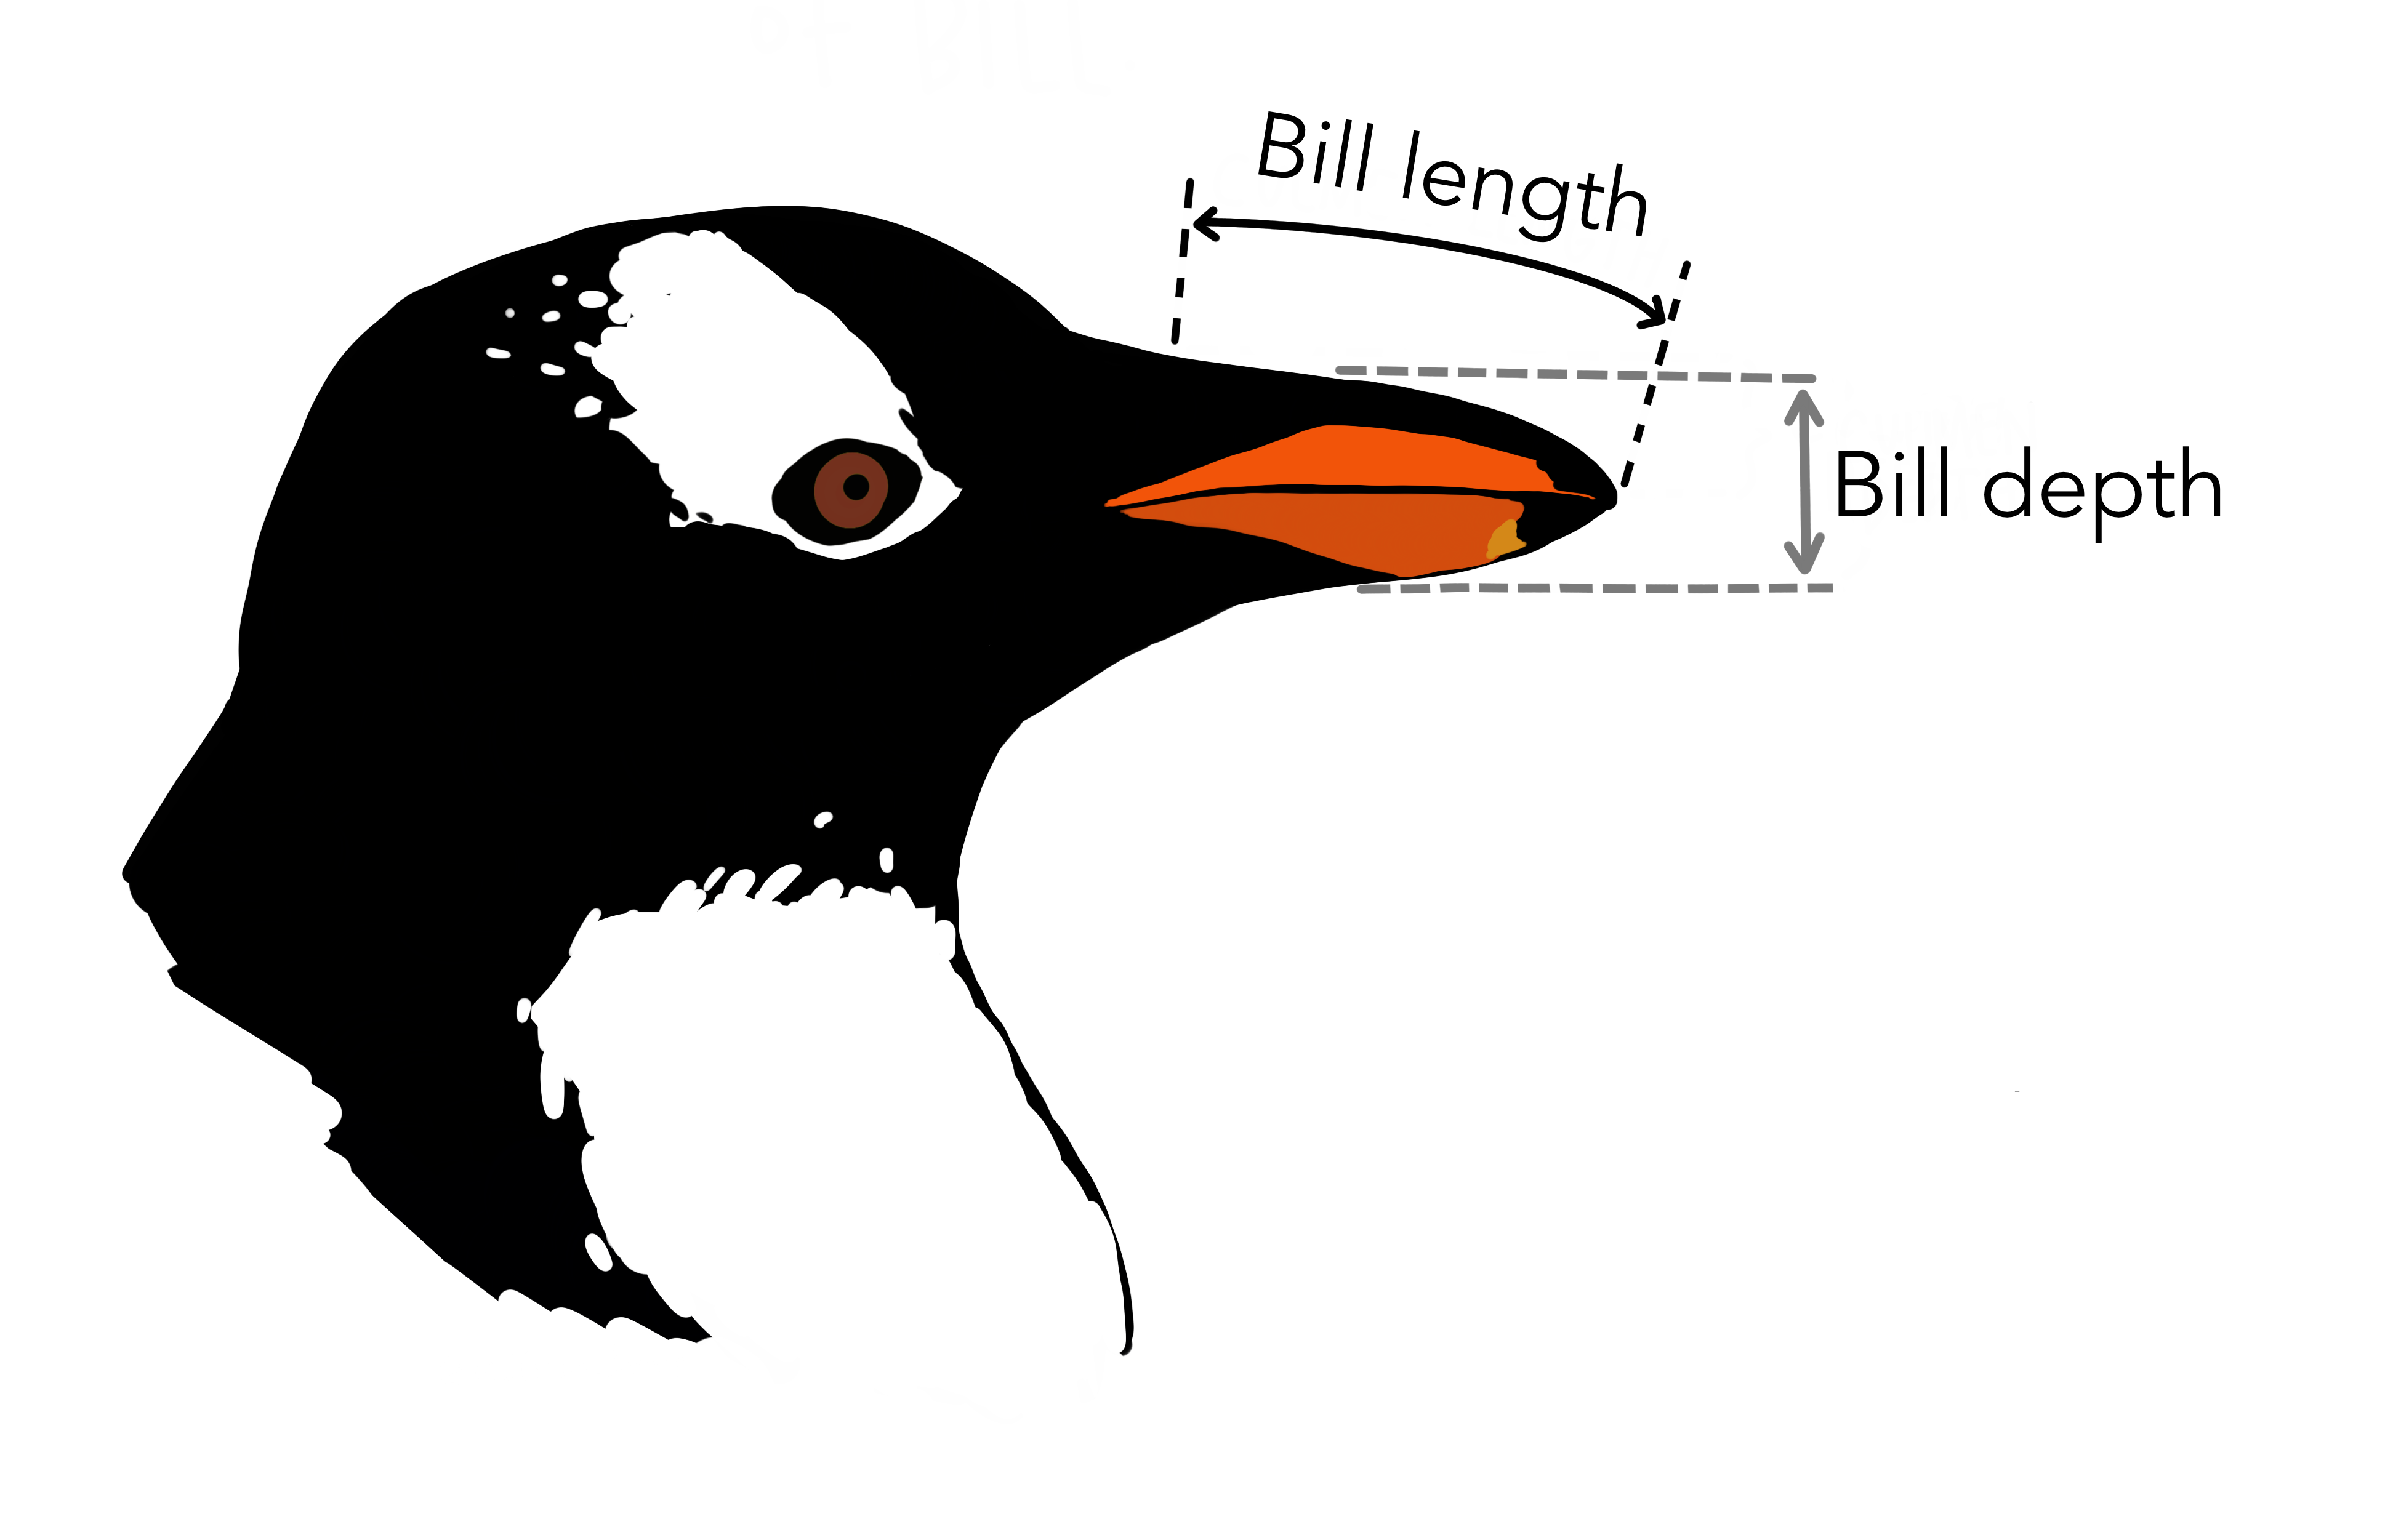
\includegraphics[width=0.5\textwidth,height=\textheight]{./images/culmen_depth.png}

}

\caption{\label{fig-morpho}Morphométrie du bec des manchots.
Illustration de Allison Horst}

\end{figure}

Supposons qu'on cherche à déterminer si la longueur du bec des manchots
est proportionnelle à leur masse. Pour produire un graphique permettant
de le déterminer, nous avons besoin des éléments suivants :

\begin{enumerate}
\def\labelenumi{\arabic{enumi}.}
\tightlist
\item
  \texttt{data} : le tableau \texttt{penguins}
\item
  un objet géométrique, ici, des points (\texttt{geom\_point()}) puisque
  nous disposons de 2 variables numériques (plus de détails à ce sujet
  plus bas)
\item
  l'association de certaines variables du jeu de données (ici,
  \texttt{body\_mass\_g} et \texttt{bill\_length\_mm}) à certaines
  caractéristiques esthétiques du graphiques (ici, la position sur les
  axes des \texttt{x} et des \texttt{y}), grâce à l'argument
  \texttt{mapping} et la fonction \texttt{aes()}.
\end{enumerate}

Concrètement, voilà le code qu'il faut taper dans votre script :

\begin{Shaded}
\begin{Highlighting}[]
\FunctionTok{ggplot}\NormalTok{(}\AttributeTok{data =}\NormalTok{ penguins, }\AttributeTok{mapping =} \FunctionTok{aes}\NormalTok{(}\AttributeTok{x =}\NormalTok{ body\_mass\_g, }\AttributeTok{y =}\NormalTok{ bill\_length\_mm))}
\end{Highlighting}
\end{Shaded}

\begin{figure}[H]

{\centering 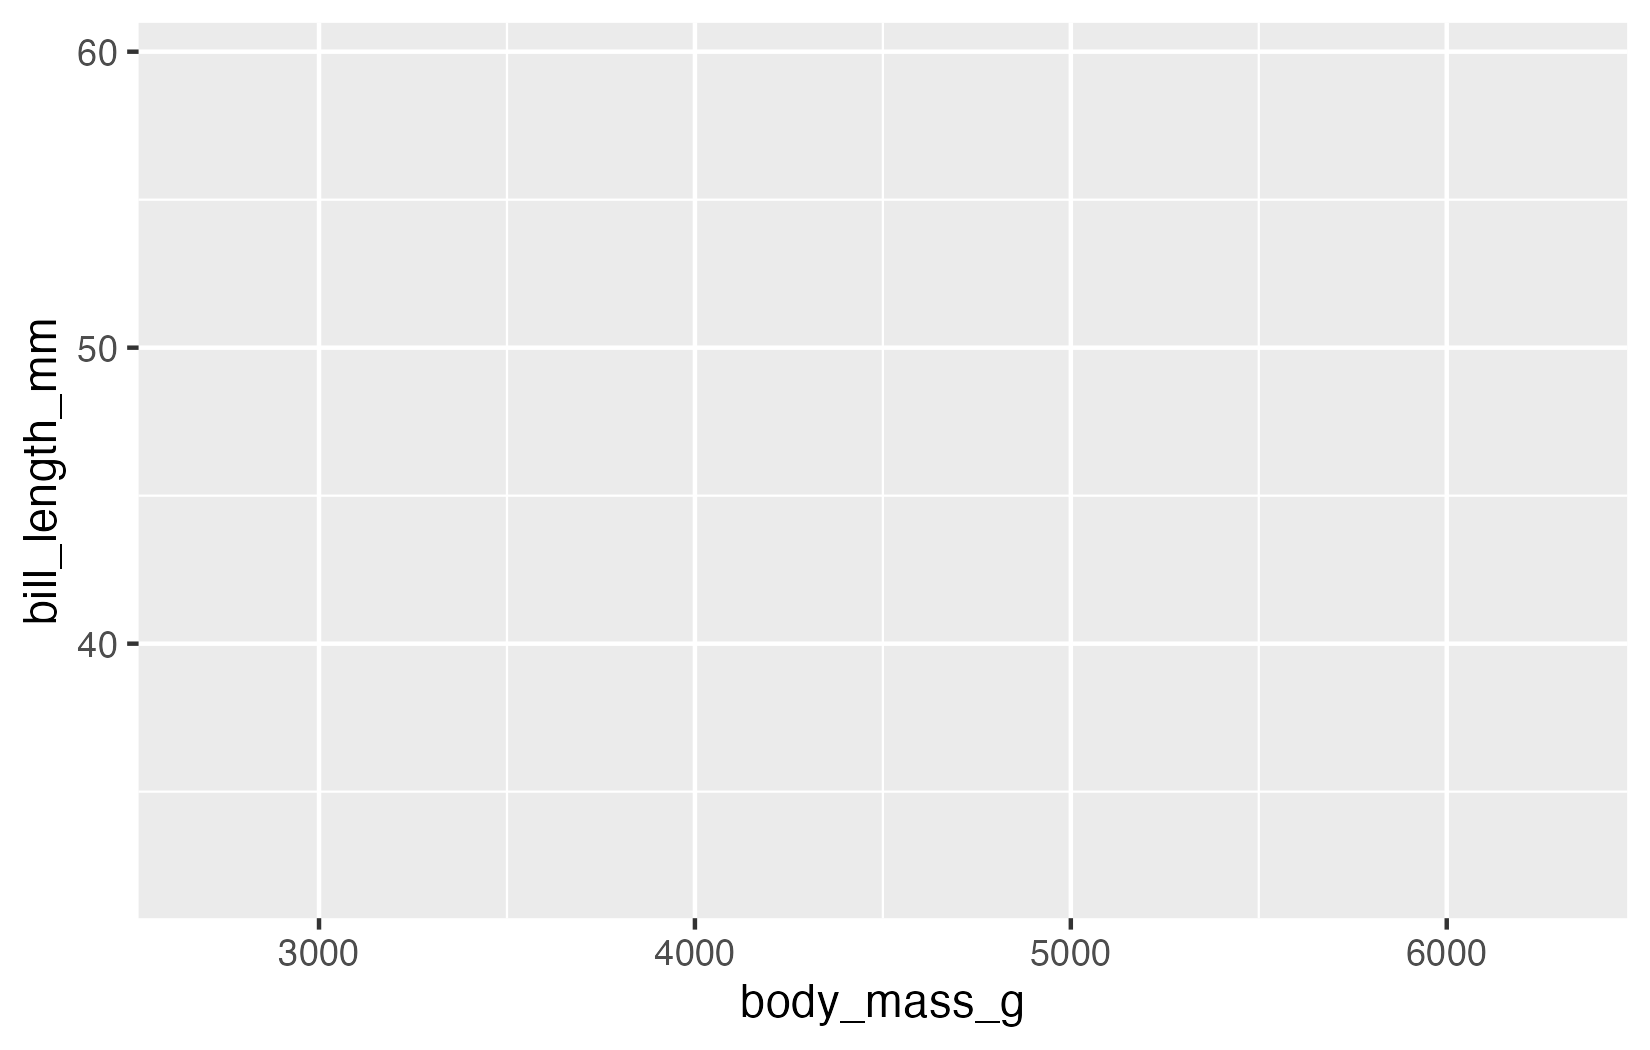
\includegraphics{./03-visualization_files/figure-pdf/unnamed-chunk-5-1.png}

}

\end{figure}

Cette première ligne de code permet de faire plusieurs choses :

\begin{enumerate}
\def\labelenumi{\arabic{enumi}.}
\tightlist
\item
  on indique à \texttt{R} qu'on souhaite faire un graphique (avec la
  fonction \texttt{ggplot()})
\item
  on indique à \texttt{R} que les données sont contenues dans l'objet
  \texttt{penguins} avec \texttt{data\ =\ penguins}
\item
  on associe (avec \texttt{mapping\ =} la variable
  \texttt{body\_mass\_g} à l'axe des \texttt{x} et la variable
  \texttt{bill\_length\_mm} à l'axe des \texttt{y}. On fait cela grâce à
  \texttt{aes(x\ =\ body\_mass\_g,\ y\ =\ bill\_length\_mm)}
\end{enumerate}

Cette commande génère la première couche du graphique. Il n'y a pas
encore de données car nous n'avons pas indiqué quel type d'objet
géométrique nous souhaitons afficher, mais la fenêtre graphique est bel
et bien créée, les axes apparaissent, ils sont légendés et leur échelle
est adaptée aux variables du tableau \texttt{penguins} que nous avons
sélectionnées. Pour terminer le graphique, il nous faut donc ajouter une
seconde couche, celle de l'objet géométrique :

\begin{Shaded}
\begin{Highlighting}[]
\FunctionTok{ggplot}\NormalTok{(}\AttributeTok{data =}\NormalTok{ penguins, }\AttributeTok{mapping =} \FunctionTok{aes}\NormalTok{(}\AttributeTok{x =}\NormalTok{ body\_mass\_g, }\AttributeTok{y =}\NormalTok{ bill\_length\_mm)) }\SpecialCharTok{+}
  \FunctionTok{geom\_point}\NormalTok{()}
\end{Highlighting}
\end{Shaded}

\begin{verbatim}
Warning: Removed 2 rows containing missing values (geom_point).
\end{verbatim}

\begin{figure}[H]

{\centering 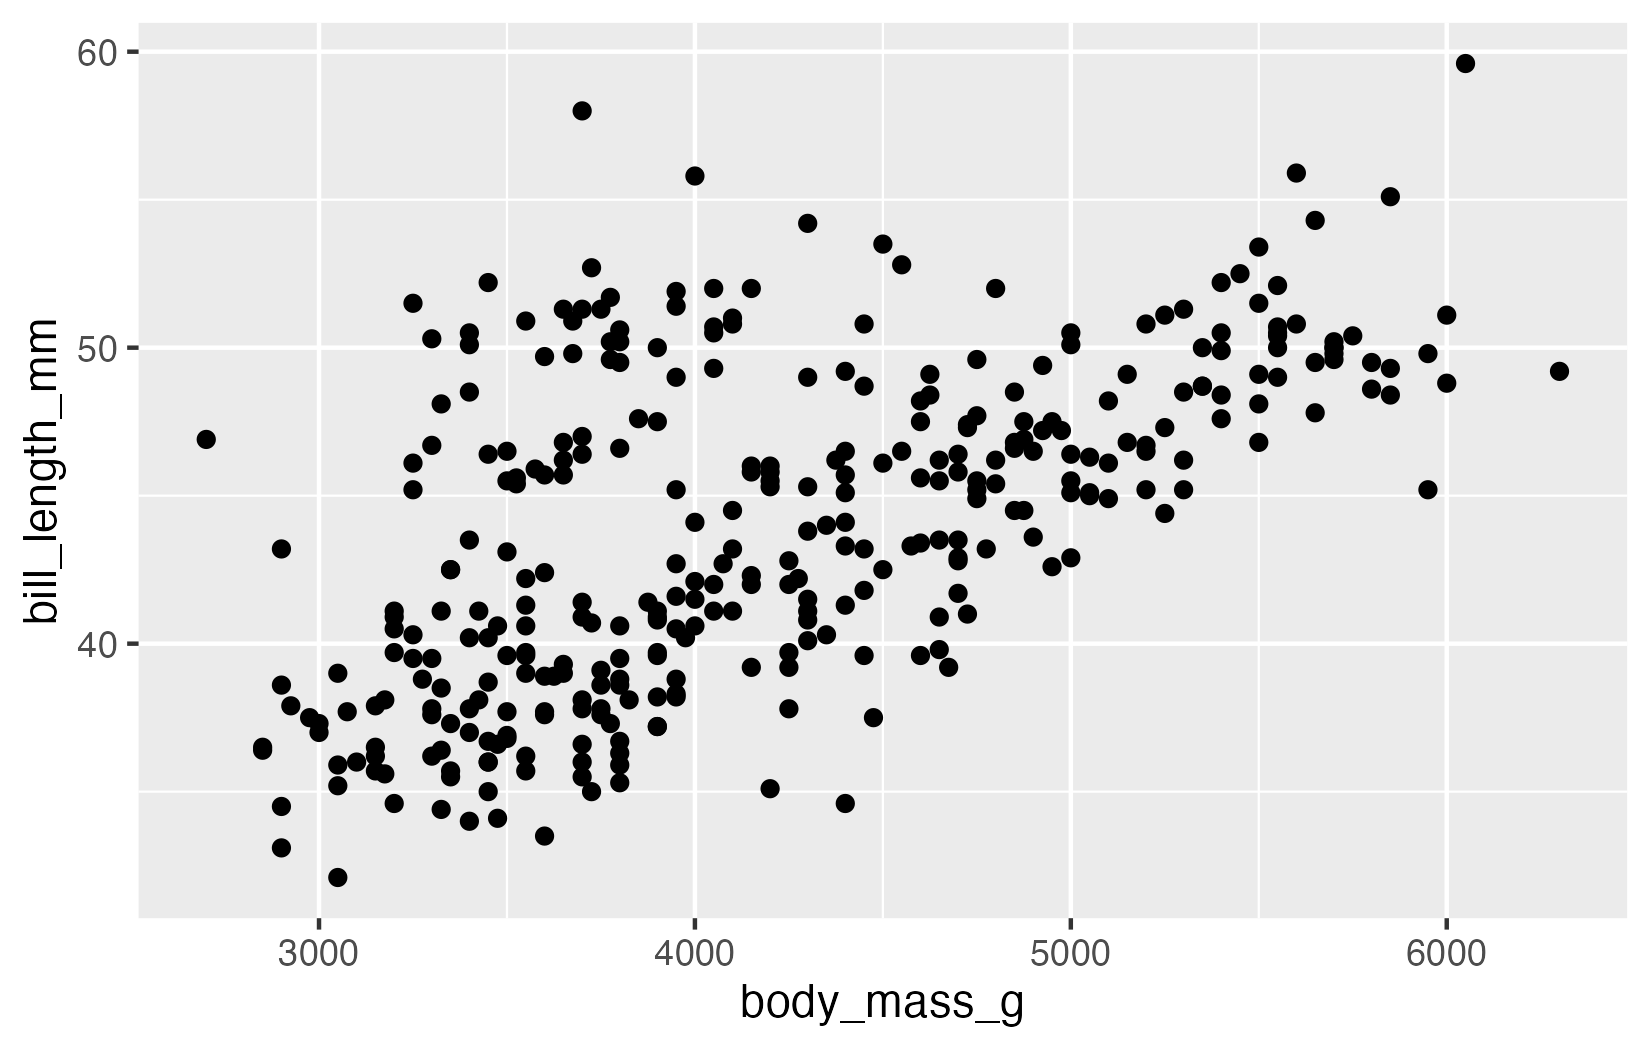
\includegraphics{./03-visualization_files/figure-pdf/unnamed-chunk-6-1.png}

}

\caption{Relation entre masse corporelle et longueur du bec chez les
manchots de l'archipel de Palmer}

\end{figure}

Au moment de produire ce graphique, \texttt{R} nous indique que 2 lignes
du tableau \texttt{penguins} ne figurent pas sur ce graphique car elles
possèdent des données manquantes (\texttt{NA}), pour l'une et/ou l'autre
des variables que nous avons sélectionnées. La fonction
\texttt{geom-point()} est donc incapable de les placer sur le graphique.

Vous avez donc ici un premier exemple de graphique très simple. Il est
loin d'être parfait (à minima, le titre des axes devrait être modifié),
mais il a le mérite de vous présenter la syntaxe que vous devrez
utiliser pour produire presque tous les graphiques qui vous seront
utiles avec \texttt{ggplot2}. En outre, on peut percevoir qu'il semble
exister une relation positive (mais imparfaite) entre longueur des becs
et masse des individus. Il faut toutefois être prudent car nous avons
ici utilisé toutes les données disponibles (donc les données des 3
espèces à la fois), ce qui est loin d'être pertinent.

\begin{tcolorbox}[enhanced jigsaw, bottomtitle=1mm, title=\textcolor{quarto-callout-tip-color}{\faLightbulb}\hspace{0.5em}{En résumé}, breakable, opacitybacktitle=0.6, coltitle=black, opacityback=0, toprule=.15mm, toptitle=1mm, titlerule=0mm, colback=white, rightrule=.15mm, arc=.35mm, leftrule=.75mm, bottomrule=.15mm, left=2mm, colframe=quarto-callout-tip-color-frame, colbacktitle=quarto-callout-tip-color!10!white]

\begin{itemize}
\tightlist
\item
  Au sein de la fonction \texttt{ggplot()}, on spécifie 2 composants de
  la grammaire des graphiques :

  \begin{enumerate}
  \def\labelenumi{\arabic{enumi}.}
  \tightlist
  \item
    le nom du tableau contenant les données grâce à l'argument
    \texttt{data\ =\ penguins}
  \item
    l'association (\texttt{mapping}) des variables du tableau de données
    à des caractéristiques esthétiques (\texttt{aes()}) en précisant
    \texttt{aes(x\ =\ body\_mass\_g,\ y\ =\ bill\_length\_mm)} :

    \begin{itemize}
    \tightlist
    \item
      la variable \texttt{body\_mass\_g} est associée à l'esthétique de
      position \texttt{x}
    \item
      la variable \texttt{bill\_length\_mm} est associée à l'esthétique
      de position \texttt{y}
    \end{itemize}
  \end{enumerate}
\item
  On ajoute une couche au graphique \texttt{ggplot()} grâce au symbole
  \texttt{+}. La couche en question précise le troisième élément
  indispensable de la grammaire des graphiques : l'objet
  \texttt{geom}étrique. Ici, les objets sont des \texttt{point}s. On le
  spécifie grâce à la fonction \texttt{geom\_point()}.
\end{itemize}

\end{tcolorbox}

Quelques remarques concernant les couches :

\begin{itemize}
\tightlist
\item
  Notez que le signe \texttt{+} est placé \emph{à la fin de la ligne}.
  Vous recevrez un message d'erreur si vous le placez au début.
\item
  Quand vous ajoutez une couche à un graphique, je vous encourage
  vivement à presser la touche \texttt{enter} de votre clavier juste
  après le symbole \texttt{+}. Ainsi, le code correspondant à chaque
  couche sera sur une ligne distincte, ce qui augmente considérablement
  la lisibilité de votre code.
\item
  Comme indiqué dans la Section~\ref{sec-functions}, tant que les
  arguments d'une fonction sont spécifiés dans l'ordre, on peut se
  passer d'écrire leur nom. Ainsi, les deux blocs de commande suivants
  produisent exactement le même résultat :
\end{itemize}

\begin{Shaded}
\begin{Highlighting}[]
\CommentTok{\# Le nom des arguments est précisé}
\FunctionTok{ggplot}\NormalTok{(}\AttributeTok{data =}\NormalTok{ penguins, }\AttributeTok{mapping =} \FunctionTok{aes}\NormalTok{(}\AttributeTok{x =}\NormalTok{ body\_mass\_g, }\AttributeTok{y =}\NormalTok{ bill\_length\_mm)) }\SpecialCharTok{+}
  \FunctionTok{geom\_point}\NormalTok{()}

\CommentTok{\# Le nom des arguments est omis}
\FunctionTok{ggplot}\NormalTok{(penguins, }\FunctionTok{aes}\NormalTok{(}\AttributeTok{x =}\NormalTok{ body\_mass\_g, }\AttributeTok{y =}\NormalTok{ bill\_length\_mm)) }\SpecialCharTok{+}
  \FunctionTok{geom\_point}\NormalTok{()}
\end{Highlighting}
\end{Shaded}

\hypertarget{sec-Exo-3}{%
\subsection{Exercices}\label{sec-Exo-3}}

\begin{enumerate}
\def\labelenumi{\arabic{enumi}.}
\tightlist
\item
  Donnez une raison pratique expliquant pourquoi les variables
  \texttt{body\_mass\_g} et \texttt{bill\_length\_mm} ont une relation
  positive
\item
  Quelles variables (pas nécessairement dans le tableau
  \texttt{penguins}) pourraient avoir une corrélation négative (relation
  négative) avec \texttt{body\_mass\_g} ? Pourquoi ? Rappelez-vous que
  nous étudions ici des variables numériques.
\item
  Citez les éléments de ce graphique/de ces données qui vous sautent le
  plus aux yeux ?
\item
  Créez un nouveau nuage de points en utilisant d'autres variables du
  jeu de données \texttt{penguins}
\end{enumerate}

\hypertarget{quel-graphique-dans-quelle-situation}{%
\section{Quel graphique dans quelle situation
?}\label{quel-graphique-dans-quelle-situation}}

Il n'est pas possible de faire n'importe quel type de graphique dans
n'importe quelle situation. Selon le nombre de variables dont on dispose
ou que l'on souhaite examiner, et selon la nature de ces variables
(numériques et/ou catégorielles), le choix des types de graphiques
possibles sera limité. Par exemple, les diagrammes bâtons sont réservés
aux variables catégorielles, alors que les histogrammes sont possibles
uniquement avec les variables numériques continues. Néanmoins, dans
certaines situations, plusieurs choix de graphiques seront possibles, et
vous aurez donc une certaine liberté. Vos choix seront alors guidés par
les objectifs que vous souhaiterez atteindre grâce aux graphiques, ainsi
que par vos préférences.

\begin{tcolorbox}[enhanced jigsaw, bottomtitle=1mm, title=\textcolor{quarto-callout-tip-color}{\faLightbulb}\hspace{0.5em}{Objectifs}, breakable, opacitybacktitle=0.6, coltitle=black, opacityback=0, toprule=.15mm, toptitle=1mm, titlerule=0mm, colback=white, rightrule=.15mm, arc=.35mm, leftrule=.75mm, bottomrule=.15mm, left=2mm, colframe=quarto-callout-tip-color-frame, colbacktitle=quarto-callout-tip-color!10!white]
Dans la suite de ce chapitre, nous traiterons donc des situations les
plus courantes : quel(s) type(s) de graphique(s) produire lorsque l'on
dispose d'une, deux ou trois variables ? Quel(s) type(s) de graphique(s)
produire lorsque les variables sont toutes numériques, toutes
catégorielles, ou lorsqu'on dispose de variables des deux types ?

Pour chaque situation, un ou des exemples seront fournis à partir des
données du tableau \texttt{penguins}. Cela sera aussi l'occasion de
présenter quelques subtilités liées à l'utilisation du package
\texttt{ggplot2}.
\end{tcolorbox}

\hypertarget{une-seule-variable-numuxe9rique}{%
\section{Une seule variable
numérique}\label{une-seule-variable-numuxe9rique}}

Lorsque l'on souhaite examiner une unique variable numérique, deux types
de représentations graphiques sont en général possible :

\begin{enumerate}
\def\labelenumi{\arabic{enumi}.}
\tightlist
\item
  les histogrammes : la variable d'intérêt est placée sur l'axe des
  \texttt{x} du graphique. Les valeurs utilisées sur l'axe des
  \texttt{y} est calculée automatiquement par le logiciel.
\item
  les nuages de points : la variable d'intérêt est placée sur l'axe des
  \texttt{y}. L'axe des \texttt{x} porte soit un simple numéro d'indice
  pour chaque observation, soit une unique valeur sans importance.
\end{enumerate}

Les syntaxes et options pour ces 2 types de graphiques sont présentées
ci-dessous.

\hypertarget{les-histogrammes}{%
\subsection{Les histogrammes}\label{les-histogrammes}}

\hypertarget{syntaxe-uxe9luxe9mentaire}{%
\subsubsection{Syntaxe élémentaire}\label{syntaxe-uxe9luxe9mentaire}}

Imaginons que l'on s'intéresse à la variable \texttt{body\_mass\_g} du
jeu de données \texttt{penguins}.

La syntaxe permettant de produire un histogramme, sous sa forme la plus
simple, est la suivante :

\begin{Shaded}
\begin{Highlighting}[]
\FunctionTok{ggplot}\NormalTok{(penguins, }\FunctionTok{aes}\NormalTok{(}\AttributeTok{x =}\NormalTok{ body\_mass\_g)) }\SpecialCharTok{+}
  \FunctionTok{geom\_histogram}\NormalTok{()}
\end{Highlighting}
\end{Shaded}

\begin{verbatim}
`stat_bin()` using `bins = 30`. Pick better value with `binwidth`.
\end{verbatim}

\begin{verbatim}
Warning: Removed 2 rows containing non-finite values (stat_bin).
\end{verbatim}

\begin{figure}[H]

{\centering 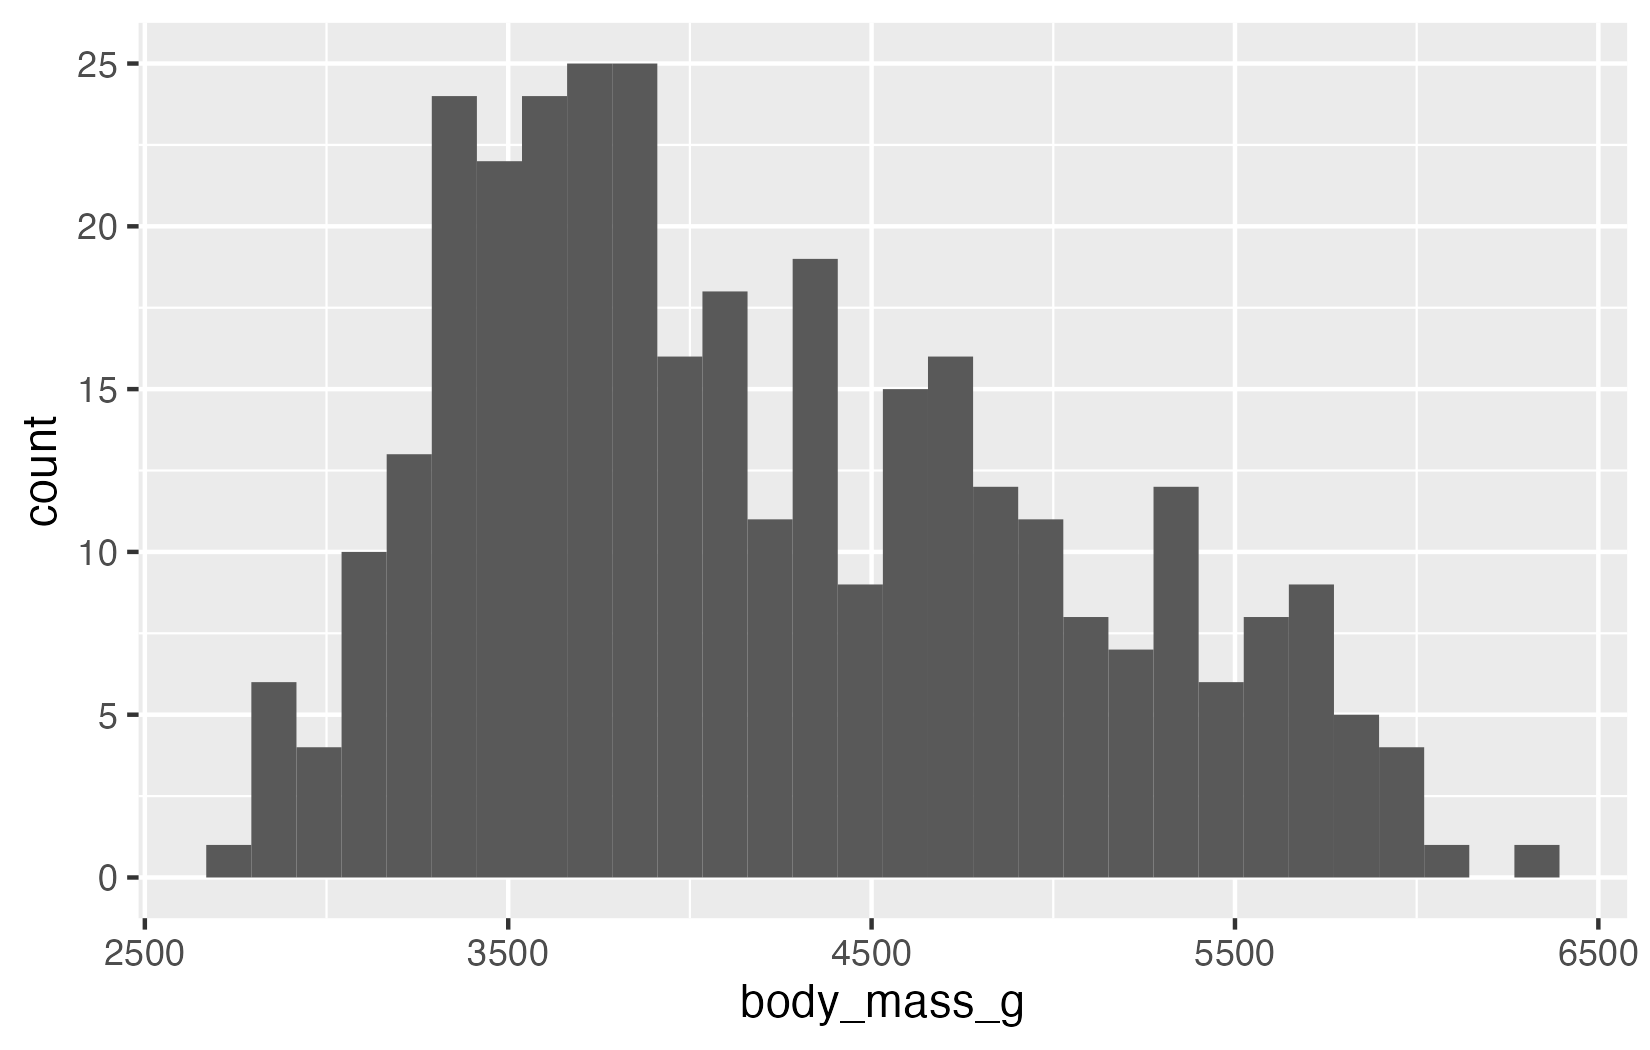
\includegraphics{./03-visualization_files/figure-pdf/unnamed-chunk-8-1.png}

}

\end{figure}

Deux messages nous sont adressés par le logiciel :

\begin{enumerate}
\def\labelenumi{\arabic{enumi}.}
\tightlist
\item
  \texttt{Message\ d\textquotesingle{}avis:\ Removed\ 2\ rows\ containing\ non-finite\ values\ (stat\_bin)}.
  Ce message indique, comme pour le premier nuage de points, que 2
  individus du tableau \texttt{penguins} ont une masse corporelle
  inconnue (\texttt{NA}). Ces 2 individus (donc les deux lignes
  correspondantes), ont été ignorés pour produire ce graphique
\item
  \texttt{\textquotesingle{}stat\_bin()\textquotesingle{}\ using\ \textquotesingle{}bins\ =\ 30\textquotesingle{}.\ Pick\ better\ value\ with\ \textquotesingle{}binwidth\textquotesingle{}}.
  Ce message indique que \texttt{R} a choisi pour nous les limites des
  classes utilisées pour faire l'histogramme. Sur un histogramme, la
  variable d'intérêt (toujours numérique et continue), qui apparaît sur
  l'axe des abscisses, est en effet ``découpée'' en plusieurs classes,
  en général de même taille, afin de permettre une représentation de la
  \textbf{distribution des valeurs}. Ici, \texttt{R} indique qu'il a
  créé 30 catégories pour nous, et que nous pouvons faire un choix
  différent grâce à l'argument \texttt{binwidth}. Nous y reviendrons un
  peu plus loin.
\end{enumerate}

Sur ce graphique, l'axe des abscisses porte donc la variable continue
``découpée'' en classes de mêmes largeur, et l'axe des ordonnées
renseigne sur le nombre (\texttt{count} ou fréquence absolue)
d'individus observés dans chaque classe. Les zones du graphique où les
barres sont les plus hautes indiquent donc les caractéristiques des
individus observés le plus fréquemment. À l'inverse, les barres les plus
courtes correspondent à des valeurs de masse rarement observées. Au
final, ce type de graphique permet de visualiser \textbf{la distribution
des données pour une variable numérique continue}.

Ici, on constate qu'une majorité d'individus semble avoir des masses
proches de 3500 grammes. Une autre portion non négligeable des individus
(mais moins importante) semble avoir une masse légèrement supérieure à
4500 grammes. Enfin, les masses supérieures à 6000 grammes sont très
rares. L'histogramme nous permet également de visualiser l'étendue des
données : les manchots étudiés ici ont des masses qui s'étalent d'un peu
plus de 2500 grammes à un peu moins de 6500 grammes.

\hypertarget{couleur}{%
\subsubsection{Couleur}\label{couleur}}

Pour rendre ce graphique plus facilement lisible, on peut en modifier la
couleur :

\begin{itemize}
\tightlist
\item
  la couleur de remplissage des barres peut-être spécifiée grâce à
  l'argument \texttt{fill\ =}
\item
  la couleur de contour des barres peut-être spécifiée grâce à
  l'argument \texttt{color\ =}
\end{itemize}

Une liste des couleurs disponibles dans \texttt{R} peut être affichée
dans la console en tapant :

\begin{Shaded}
\begin{Highlighting}[]
\FunctionTok{colors}\NormalTok{()}
\end{Highlighting}
\end{Shaded}

Vous pouvez voir à quelle couleur correspond chacun de ces noms
\href{http://www.stat.columbia.edu/~tzheng/files/Rcolor.pdf}{dans ce
document pdf}.

Mettons à jour notre histogramme en ajoutant un peu de couleur :

\begin{Shaded}
\begin{Highlighting}[]
\FunctionTok{ggplot}\NormalTok{(penguins, }\FunctionTok{aes}\NormalTok{(}\AttributeTok{x =}\NormalTok{ body\_mass\_g)) }\SpecialCharTok{+}
  \FunctionTok{geom\_histogram}\NormalTok{(}\AttributeTok{fill =} \StringTok{"steelblue"}\NormalTok{, }\AttributeTok{color =} \StringTok{"black"}\NormalTok{)}
\end{Highlighting}
\end{Shaded}

\begin{verbatim}
`stat_bin()` using `bins = 30`. Pick better value with `binwidth`.
\end{verbatim}

\begin{verbatim}
Warning: Removed 2 rows containing non-finite values (stat_bin).
\end{verbatim}

\begin{figure}[H]

{\centering 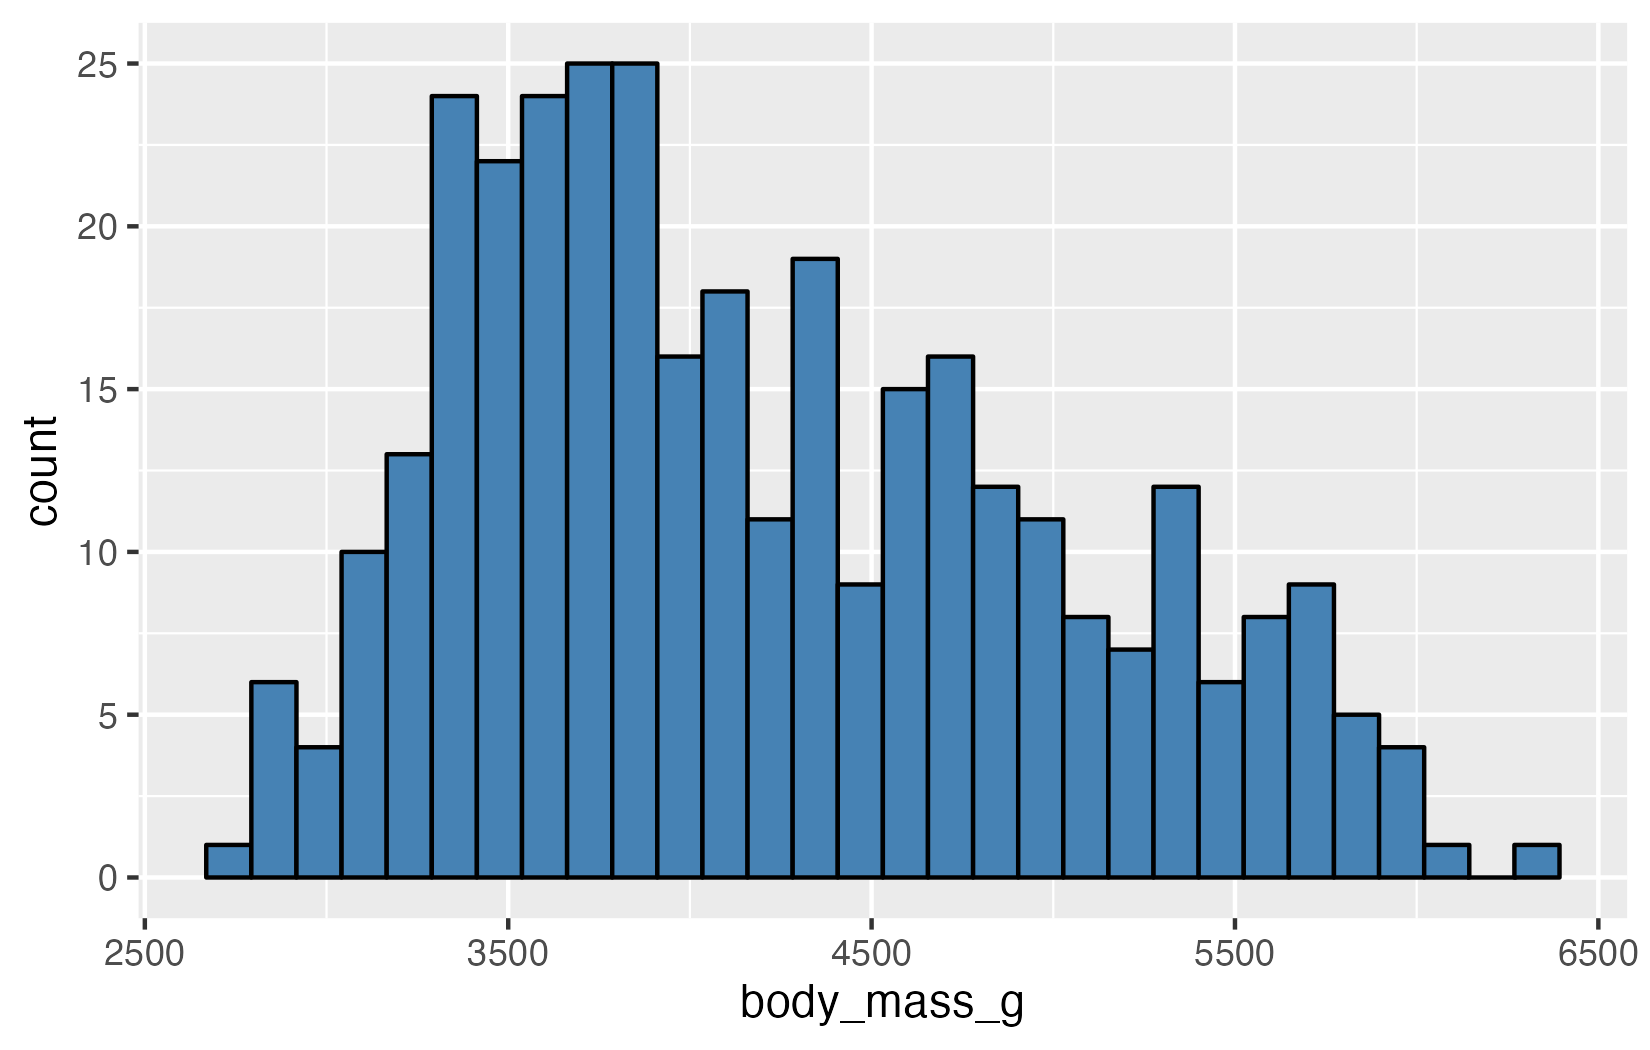
\includegraphics{./03-visualization_files/figure-pdf/unnamed-chunk-10-1.png}

}

\end{figure}

Les 30 classes de masses sont maintenant plus facilement visibles et
distingables.

\hypertarget{uxe0-lintuxe9rieur-ou-uxe0-lextuxe9rieur-de-aes}{%
\subsubsection{\texorpdfstring{À l'intérieur ou à l'extérieur de
\texttt{aes()}
?}{À l'intérieur ou à l'extérieur de aes() ?}}\label{uxe0-lintuxe9rieur-ou-uxe0-lextuxe9rieur-de-aes}}

Les couleurs de remplissage et de contour des barres d'un histogramme
font partie des caractéristiques esthétiques du graphique. Pourtant,
elles ne sont pas précisées à l'intérieur de la fonction \texttt{aes()}.
La raison est simple mais importante :

\begin{tcolorbox}[enhanced jigsaw, bottomtitle=1mm, title=\textcolor{quarto-callout-important-color}{\faExclamation}\hspace{0.5em}{Important}, breakable, opacitybacktitle=0.6, coltitle=black, opacityback=0, toprule=.15mm, toptitle=1mm, titlerule=0mm, colback=white, rightrule=.15mm, arc=.35mm, leftrule=.75mm, bottomrule=.15mm, left=2mm, colframe=quarto-callout-important-color-frame, colbacktitle=quarto-callout-important-color!10!white]
On place à l'intérieur de \texttt{aes()} uniquement les caractéristiques
esthétiques du graphique que l'on souhaite associer à des
\textbf{variables du jeu de données}.
\end{tcolorbox}

Ici, les couleurs que l'on indique sont des constantes : toutes les
barres ont les mêmes couleur de remplissage et de contour. On n'associe
pas une variable du jeu de données à ces caractéristiques esthétiques.
On place donc \texttt{fill\ =} et \texttt{color\ =} à l'extérieur de
\texttt{aes()}. Si on se trompe, voilà ce qui se produit :

\begin{Shaded}
\begin{Highlighting}[]
\FunctionTok{ggplot}\NormalTok{(penguins, }\FunctionTok{aes}\NormalTok{(}\AttributeTok{x =}\NormalTok{ body\_mass\_g)) }\SpecialCharTok{+}
  \FunctionTok{geom\_histogram}\NormalTok{(}\FunctionTok{aes}\NormalTok{(}\AttributeTok{fill =} \StringTok{"steelblue"}\NormalTok{, }\AttributeTok{color =} \StringTok{"black"}\NormalTok{))}
\end{Highlighting}
\end{Shaded}

\begin{verbatim}
`stat_bin()` using `bins = 30`. Pick better value with `binwidth`.
\end{verbatim}

\begin{verbatim}
Warning: Removed 2 rows containing non-finite values (stat_bin).
\end{verbatim}

\begin{figure}[H]

{\centering 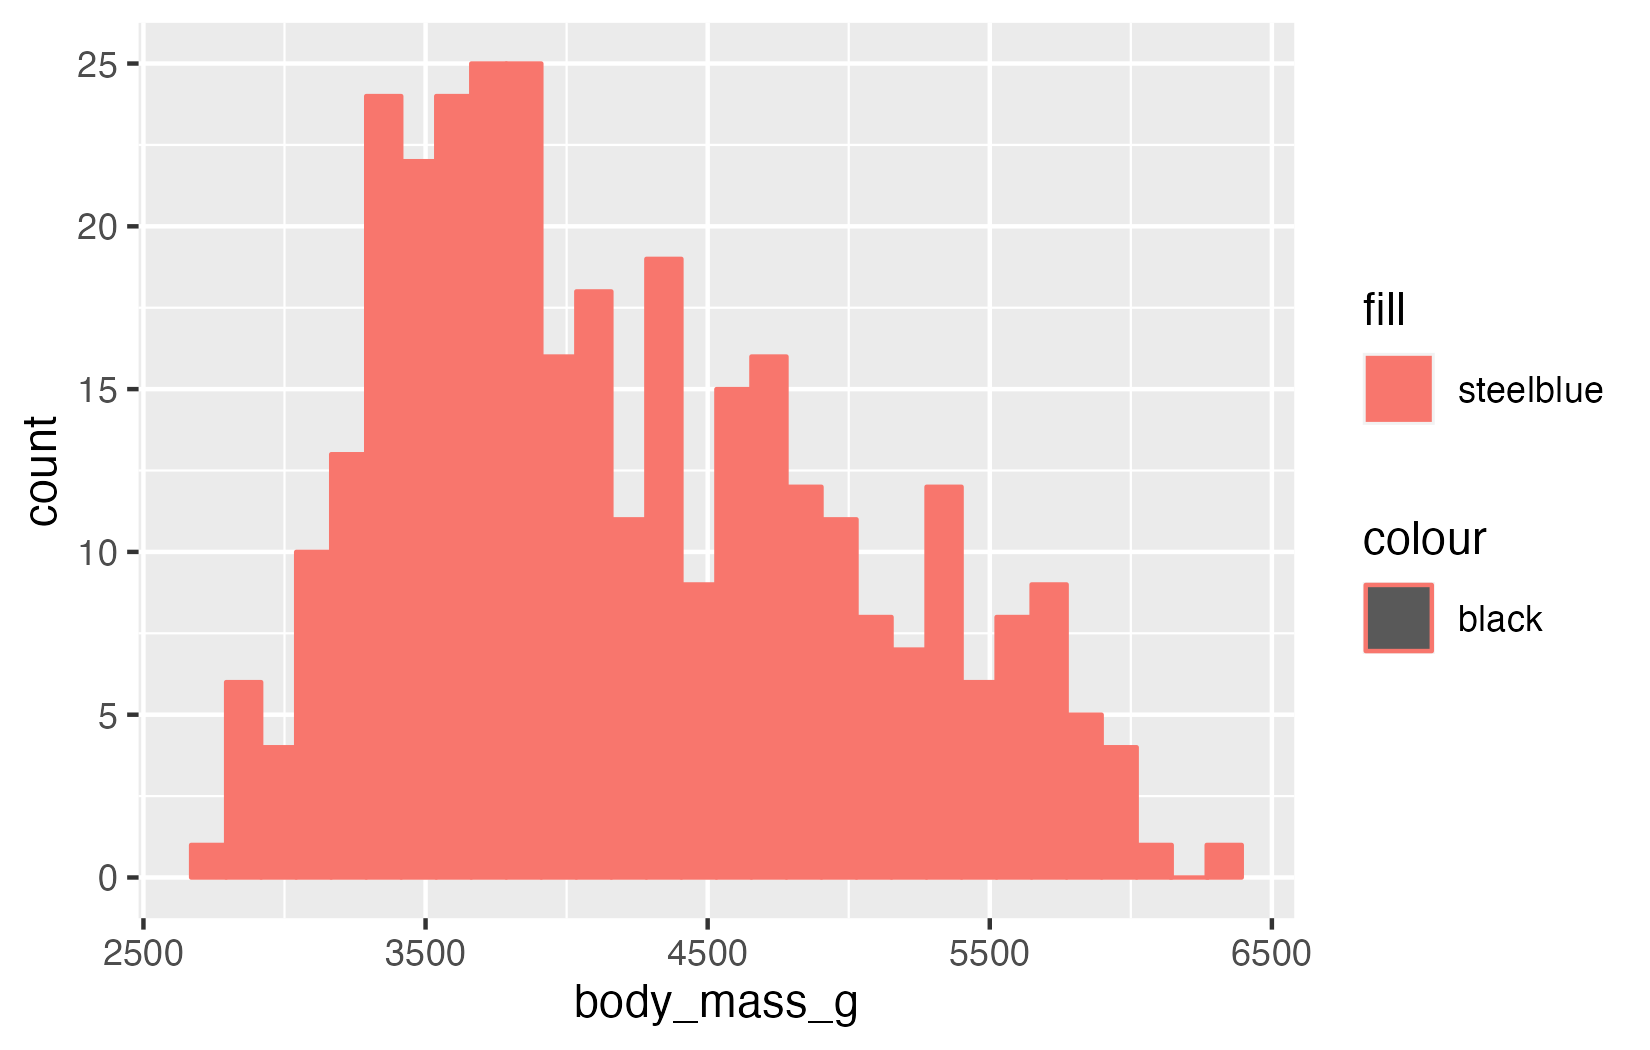
\includegraphics{./03-visualization_files/figure-pdf/unnamed-chunk-11-1.png}

}

\end{figure}

Les couleurs qui apparaissent ne correspondent pas à ce qui est demandé,
et une légende ne correspondant à rien apparaît à droite du graphique.
La syntaxe utilisée ici suppose en effet que \texttt{"steelblue"} et
\texttt{"black"} seraient des variables du jeu de données
\texttt{penguins}. Puisqu'elles n'existent pas, \texttt{R} essaie de se
débrouiller pour interpréter comme il peut ce qu'on lui demande, et
finit par produire ce graphique incohérent. La couleur utilisée est la
première couleur de la palette par défaut de \texttt{ggplot2}.

Pour élaborer des graphiques plus avancés, il faudra donc toujours vous
poser la question suivante : la caractéristique esthétique que je
souhaite modifier doit-elle être associée à une \textbf{valeur
constante} que je fixe pour toutes les barres ou tous les points d'un
graphique, et alors, je l'indique \textbf{en dehors} de \texttt{aes()},
ou est-elle au contraire associée à \textbf{une variable du jeu de
données}, et alors, je l'indique \textbf{à l'intérieur} de
\texttt{aes()}.

Il est bien sûr possible d'avoir un mélange des deux. Par exemple, le
code suivant permet d'associer la couleur de remplissage au sexe des
individus étudiés (variable \texttt{sex} du jeu de données
\texttt{penguins}), et de spécifier une valeur constante pour la couleur
de contour des barres (ici, le noir) :

\begin{Shaded}
\begin{Highlighting}[]
\FunctionTok{ggplot}\NormalTok{(penguins, }\FunctionTok{aes}\NormalTok{(}\AttributeTok{x =}\NormalTok{ body\_mass\_g)) }\SpecialCharTok{+}
  \FunctionTok{geom\_histogram}\NormalTok{(}\FunctionTok{aes}\NormalTok{(}\AttributeTok{fill =}\NormalTok{ sex), }\AttributeTok{color =} \StringTok{"black"}\NormalTok{)}
\end{Highlighting}
\end{Shaded}

\begin{verbatim}
`stat_bin()` using `bins = 30`. Pick better value with `binwidth`.
\end{verbatim}

\begin{verbatim}
Warning: Removed 2 rows containing non-finite values (stat_bin).
\end{verbatim}

\begin{figure}[H]

{\centering 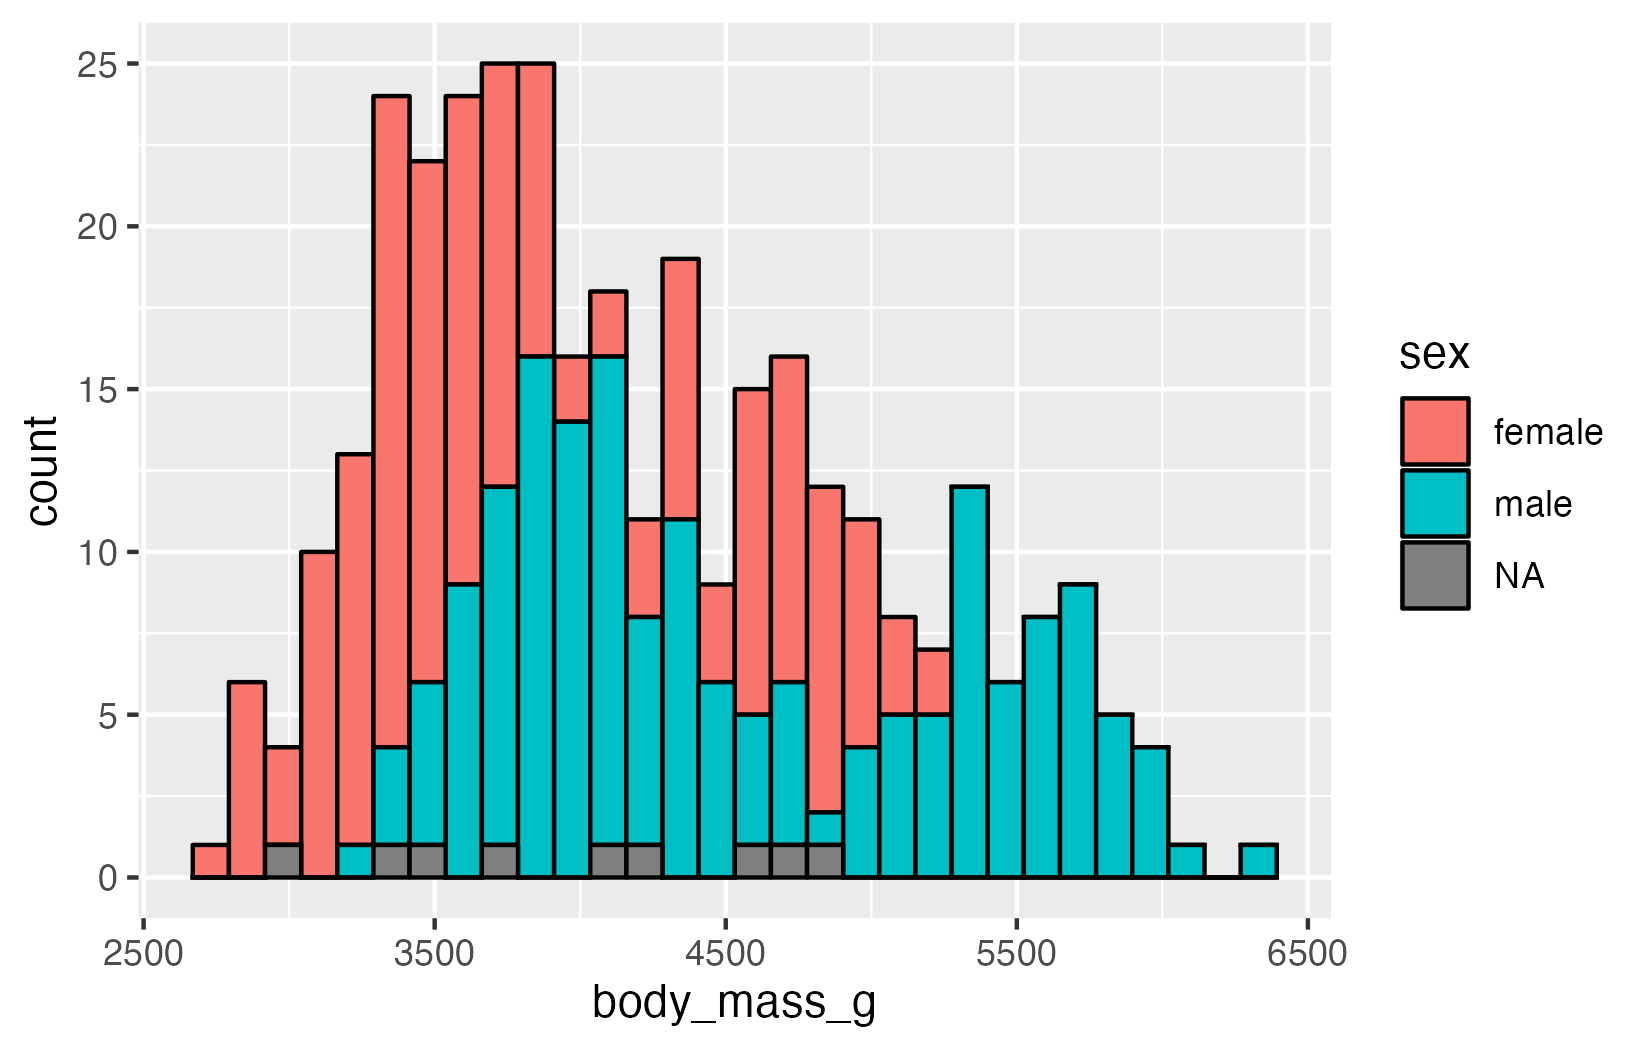
\includegraphics{./03-visualization_files/figure-pdf/unnamed-chunk-12-1.png}

}

\end{figure}

On constate que toutes les barres ont un contour noir, mais que
plusieurs couleurs de remplissage apparaissent maintenant, selon le sexe
des individus, dans chaque classe de masse. Une légende adaptée est
aussi créée automatiquement à droite du graphique. On apprend ainsi que
les individus les plus lourds sont tous des mâles. On constate également
que le sexe de certains individus est inconnu.

Au final, nous ne sommes déjà plus dans la situation où on examine une
unique variable numérique. Nous avons en effet ici un graphique nous
permettant de mettre en relation une variable numérique (la masse des
individus en grammes) et une variable catégorielle (le sexe des
individus). Nous reviendrons plus tard sur ce type de graphiques.

\hypertarget{la-largeur-des-classes}{%
\subsubsection{La largeur des classes}\label{la-largeur-des-classes}}

Comme évoqué plus haut, par défaut, \texttt{R} choisit arbitrairement de
découper la variable numérique utilisée en 30 classes de même largeur
afin de produire l'histogramme. Ça n'est que rarement un bon choix, et
malheureusement, il n'y a pas de règle permettant de définir à coup sûr
le bon nombre de classes pour visualiser au mieux la distribution d'une
variable numérique. Il faut en effet presque toujours procéder par
essais-erreurs successifs. Il est possible d'ajuster les
caractéristiques (nombre et/ou largeur) des classes de l'histogramme de
l'une des 3 façons suivantes :

\begin{enumerate}
\def\labelenumi{\arabic{enumi}.}
\tightlist
\item
  En ajustant le nombre de classes avec \texttt{bins}.
\item
  En précisant la largeur des classes avec \texttt{binwidth}.
\item
  En fournissant manuellement les limites des classes avec
  \texttt{breaks}.
\end{enumerate}

\begin{Shaded}
\begin{Highlighting}[]
\FunctionTok{ggplot}\NormalTok{(penguins, }\FunctionTok{aes}\NormalTok{(}\AttributeTok{x =}\NormalTok{ body\_mass\_g)) }\SpecialCharTok{+}
  \FunctionTok{geom\_histogram}\NormalTok{(}\AttributeTok{fill =} \StringTok{"steelblue"}\NormalTok{, }\AttributeTok{color =} \StringTok{"black"}\NormalTok{,}
                 \AttributeTok{bins =} \DecValTok{10}\NormalTok{)}
\end{Highlighting}
\end{Shaded}

\begin{verbatim}
Warning: Removed 2 rows containing non-finite values (stat_bin).
\end{verbatim}

\begin{figure}[H]

{\centering 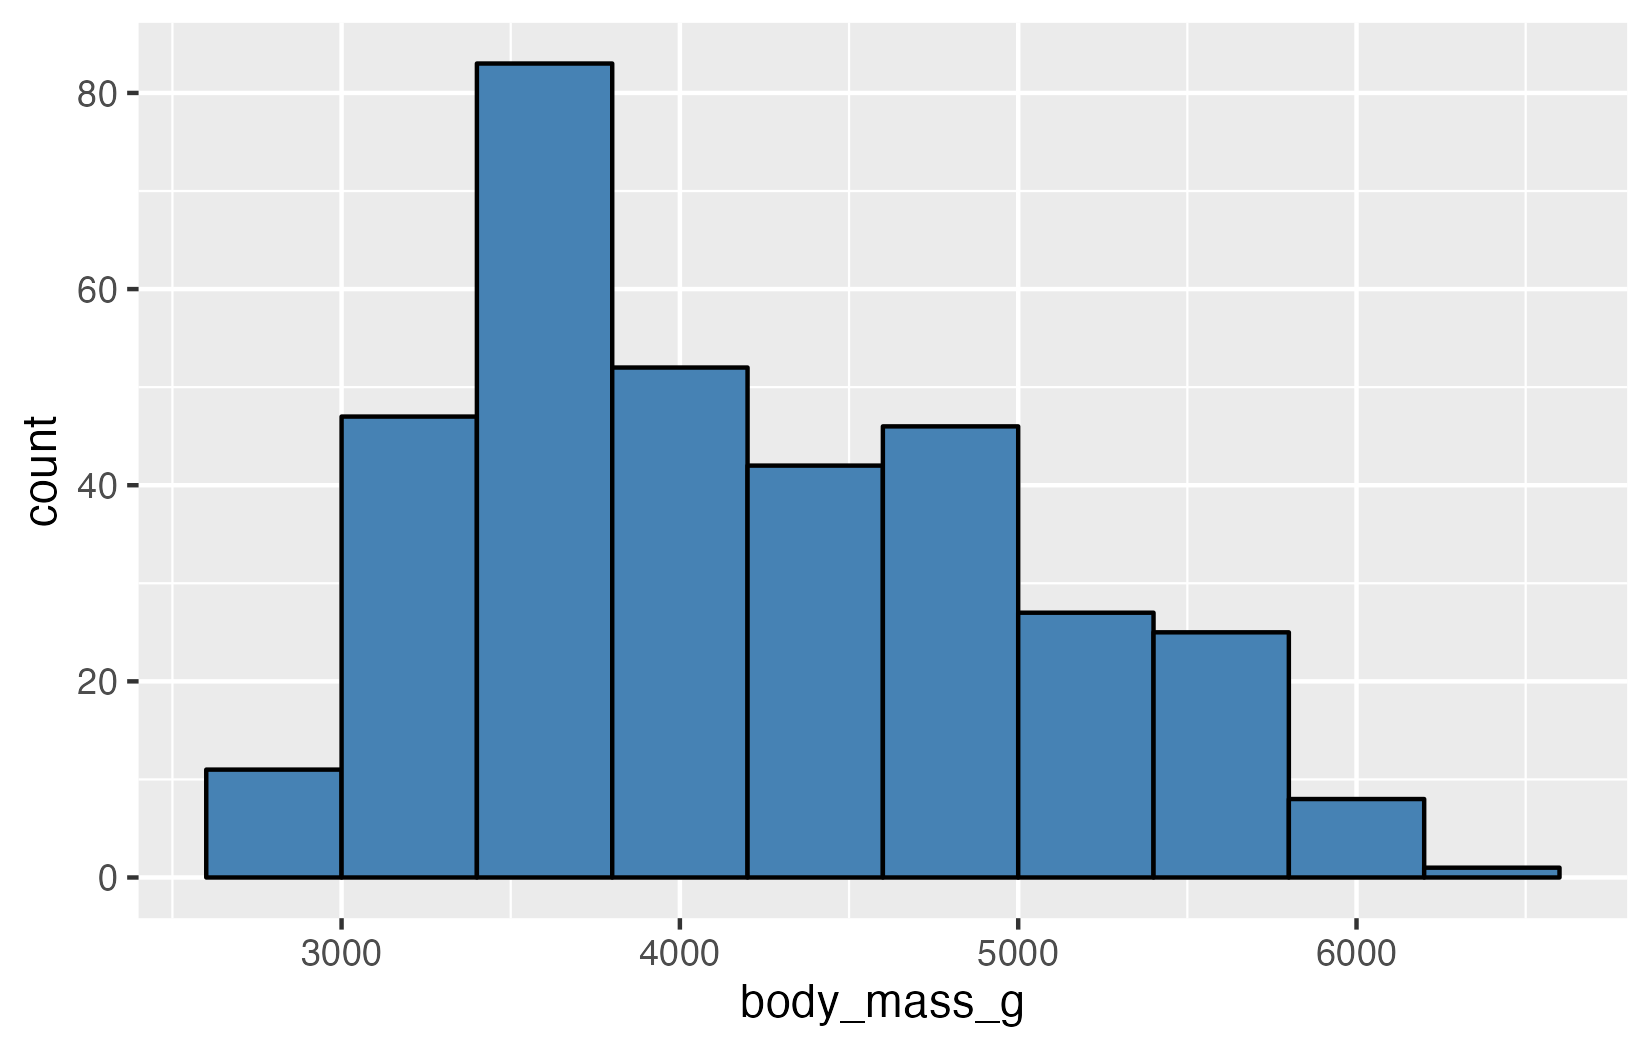
\includegraphics{./03-visualization_files/figure-pdf/unnamed-chunk-13-1.png}

}

\end{figure}

Ici, diminuer le nombre de classes à 10 a pour effet de trop lisser la
distribution des données. On ne visualise plus les variations subtiles
de la distribution. À l'inverse, trop augmenter le nombre de classes
n'est pas pertinent non plus :

\begin{Shaded}
\begin{Highlighting}[]
\FunctionTok{ggplot}\NormalTok{(penguins, }\FunctionTok{aes}\NormalTok{(}\AttributeTok{x =}\NormalTok{ body\_mass\_g)) }\SpecialCharTok{+}
  \FunctionTok{geom\_histogram}\NormalTok{(}\AttributeTok{fill =} \StringTok{"steelblue"}\NormalTok{, }\AttributeTok{color =} \StringTok{"black"}\NormalTok{,}
                 \AttributeTok{bins =} \DecValTok{100}\NormalTok{)}
\end{Highlighting}
\end{Shaded}

\begin{verbatim}
Warning: Removed 2 rows containing non-finite values (stat_bin).
\end{verbatim}

\begin{figure}[H]

{\centering 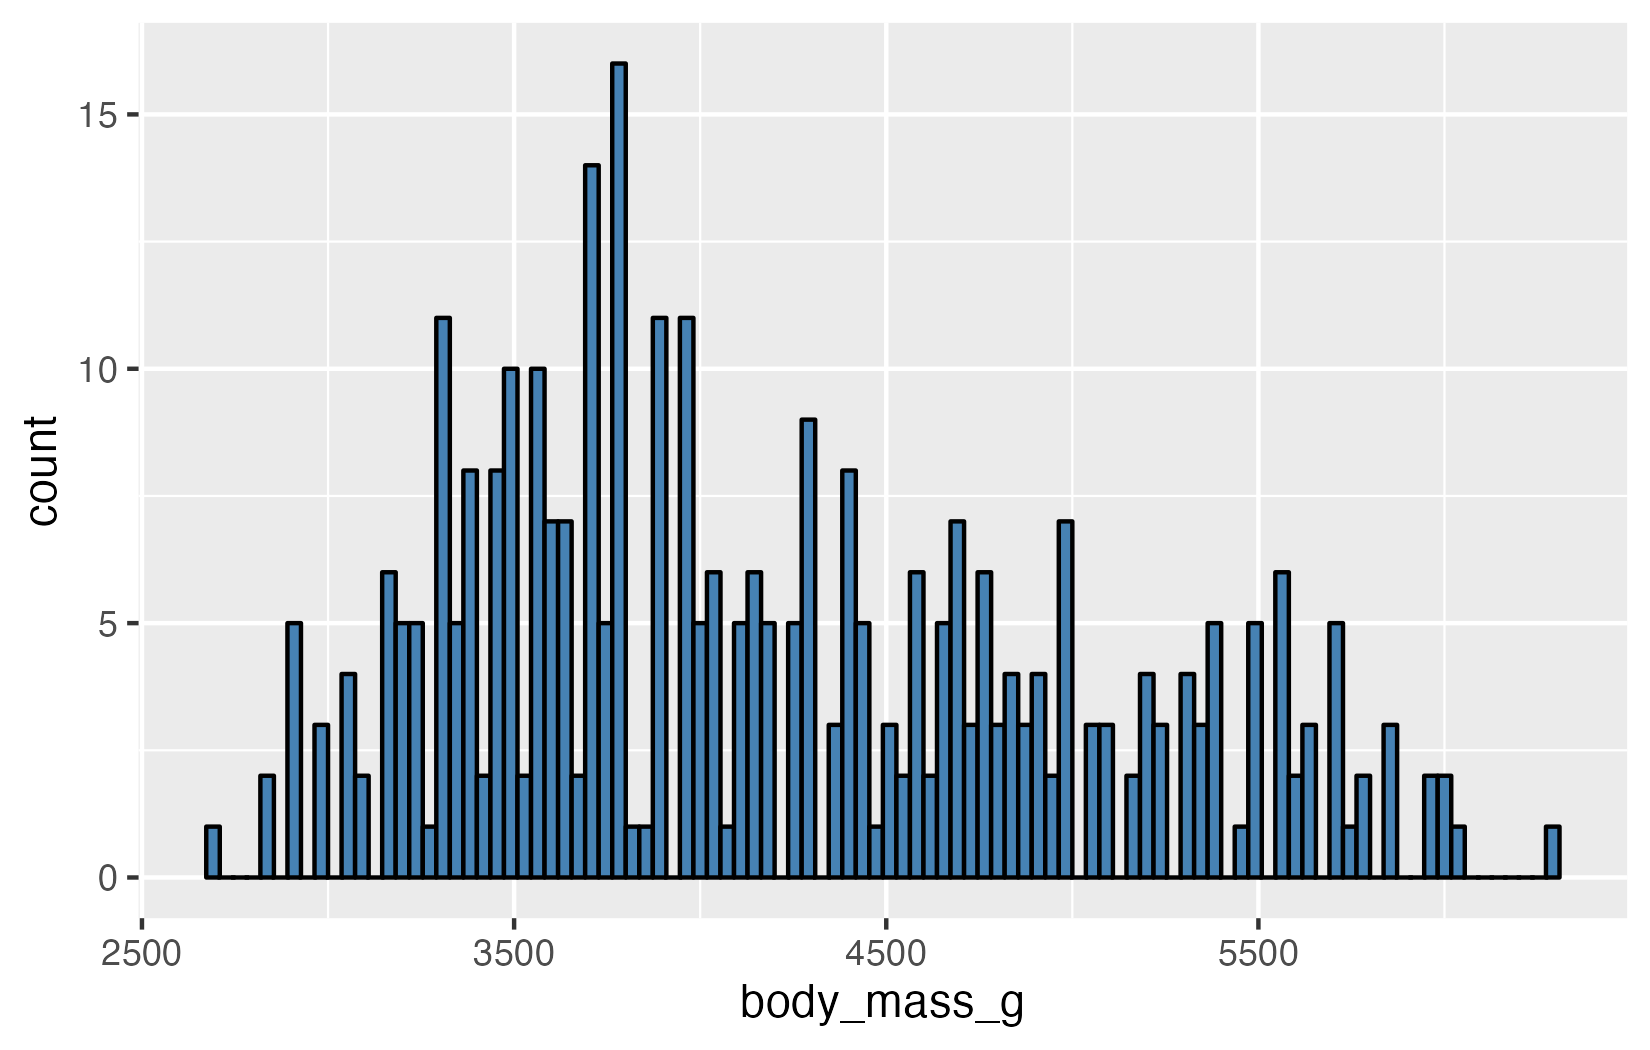
\includegraphics{./03-visualization_files/figure-pdf/unnamed-chunk-14-1.png}

}

\end{figure}

Ici, passer à 100 classes de taille génère un histogramme plein de
trous, avec des classes très étroites, dont certaines sont très
représentées, et immédiatement suivies ou précédées par des classes très
peu représentées. Cela n'a pas de logique, et c'est presque toujours le
signe qu'il faut réduire le nombre de classes.

Au final, pour ces données, un nombre de classes compris entre 20 et 30
semble un bon choix :

\begin{Shaded}
\begin{Highlighting}[]
\FunctionTok{ggplot}\NormalTok{(penguins, }\FunctionTok{aes}\NormalTok{(}\AttributeTok{x =}\NormalTok{ body\_mass\_g)) }\SpecialCharTok{+}
  \FunctionTok{geom\_histogram}\NormalTok{(}\AttributeTok{fill =} \StringTok{"steelblue"}\NormalTok{, }\AttributeTok{color =} \StringTok{"black"}\NormalTok{,}
                 \AttributeTok{bins =} \DecValTok{25}\NormalTok{)}
\end{Highlighting}
\end{Shaded}

\begin{verbatim}
Warning: Removed 2 rows containing non-finite values (stat_bin).
\end{verbatim}

\begin{figure}[H]

{\centering 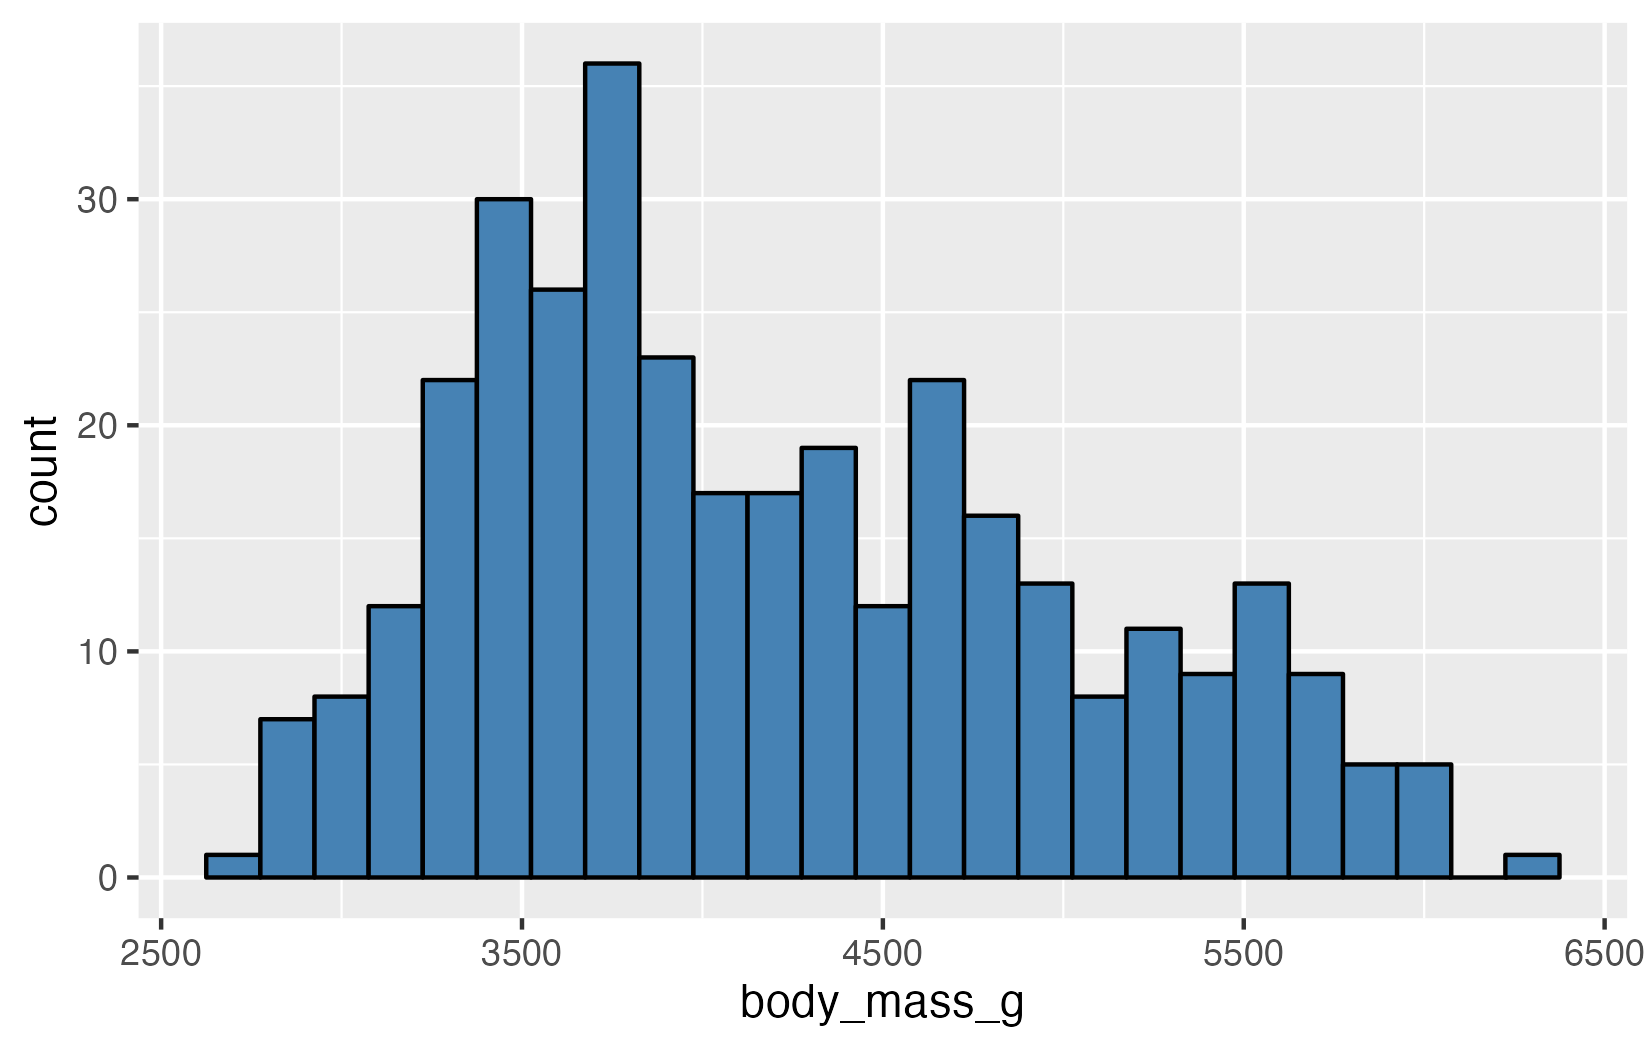
\includegraphics{./03-visualization_files/figure-pdf/unnamed-chunk-15-1.png}

}

\end{figure}

C'est un bon choix, entre trop peu d'information, et trop de bruit
visuel. Évidemment, ce nombre sera différent pour chaque jeu de données.
On constate ici à peu près 3 pics (autour de 3500 grammes, un peu
au-dessus de 4500 grammes, et autour de 5500 grammes) qui reflètent bien
la distribution de ces données.

On peut également modifier \textbf{la largeur des classes} (et non plus
leur nombre) avec \texttt{binwidth} :

\begin{Shaded}
\begin{Highlighting}[]
\FunctionTok{ggplot}\NormalTok{(penguins, }\FunctionTok{aes}\NormalTok{(}\AttributeTok{x =}\NormalTok{ body\_mass\_g)) }\SpecialCharTok{+}
  \FunctionTok{geom\_histogram}\NormalTok{(}\AttributeTok{fill =} \StringTok{"steelblue"}\NormalTok{, }\AttributeTok{color =} \StringTok{"black"}\NormalTok{,}
                 \AttributeTok{binwidth =} \DecValTok{200}\NormalTok{)}
\end{Highlighting}
\end{Shaded}

\begin{verbatim}
Warning: Removed 2 rows containing non-finite values (stat_bin).
\end{verbatim}

\begin{figure}[H]

{\centering 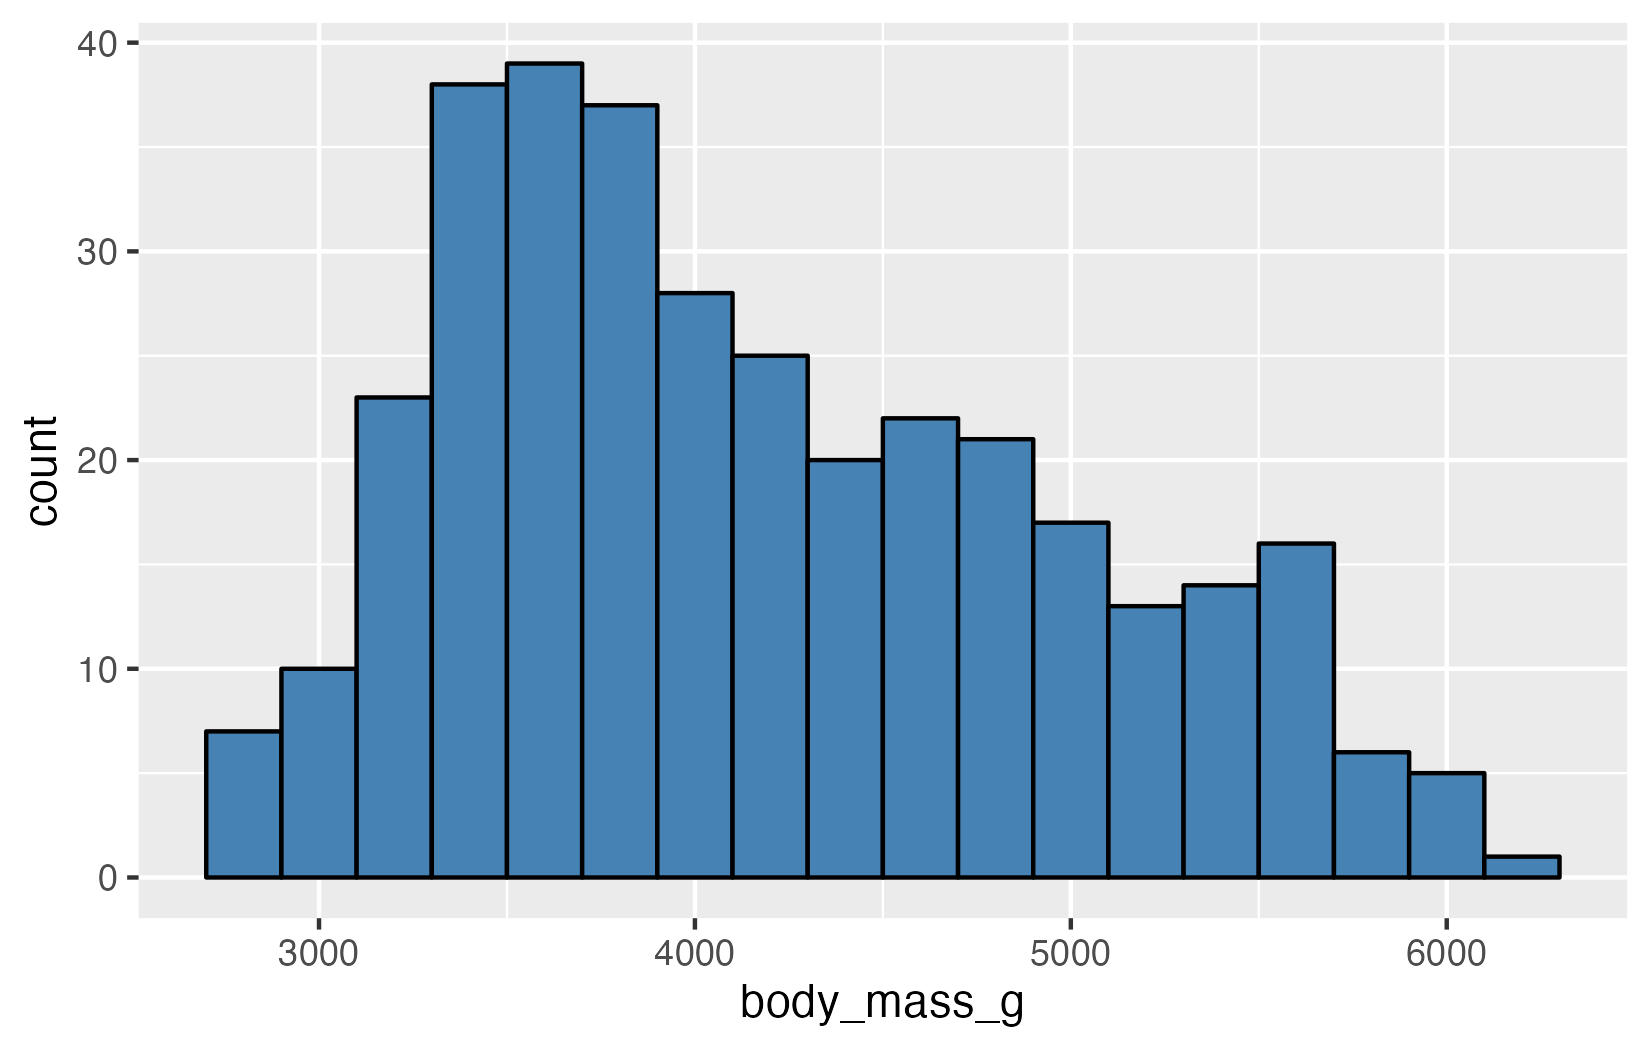
\includegraphics{./03-visualization_files/figure-pdf/unnamed-chunk-16-1.png}

}

\end{figure}

Ici, chaque catégorie recouvre 200 grammes. Avec l'argument
\texttt{bins}, on indique à \texttt{R} combien on souhaite obtenir de
classes, et il détermine automatiquement leur largeur. Avec
\texttt{binwidth}, on indique la largeur des classes souhaitées, et
\texttt{R} détermine automatiquement le nombre de classes nécessaires
pour couvrir la totalité des données.

Enfin, il est possible de déterminer manuellement les limites des
classes souhaitées avec l'argument \texttt{breaks} :

\begin{Shaded}
\begin{Highlighting}[]
\FunctionTok{ggplot}\NormalTok{(penguins, }\FunctionTok{aes}\NormalTok{(}\AttributeTok{x =}\NormalTok{ body\_mass\_g)) }\SpecialCharTok{+}
  \FunctionTok{geom\_histogram}\NormalTok{(}\AttributeTok{fill =} \StringTok{"steelblue"}\NormalTok{, }\AttributeTok{color =} \StringTok{"black"}\NormalTok{,}
                 \AttributeTok{breaks =} \FunctionTok{c}\NormalTok{(}\DecValTok{2500}\NormalTok{, }\DecValTok{2750}\NormalTok{, }\DecValTok{3000}\NormalTok{, }\DecValTok{3500}\NormalTok{, }\DecValTok{4000}\NormalTok{, }\DecValTok{4500}\NormalTok{, }\DecValTok{5000}\NormalTok{, }\DecValTok{6000}\NormalTok{, }\DecValTok{7000}\NormalTok{))}
\end{Highlighting}
\end{Shaded}

\begin{verbatim}
Warning: Removed 2 rows containing non-finite values (stat_bin).
\end{verbatim}

\begin{figure}[H]

{\centering 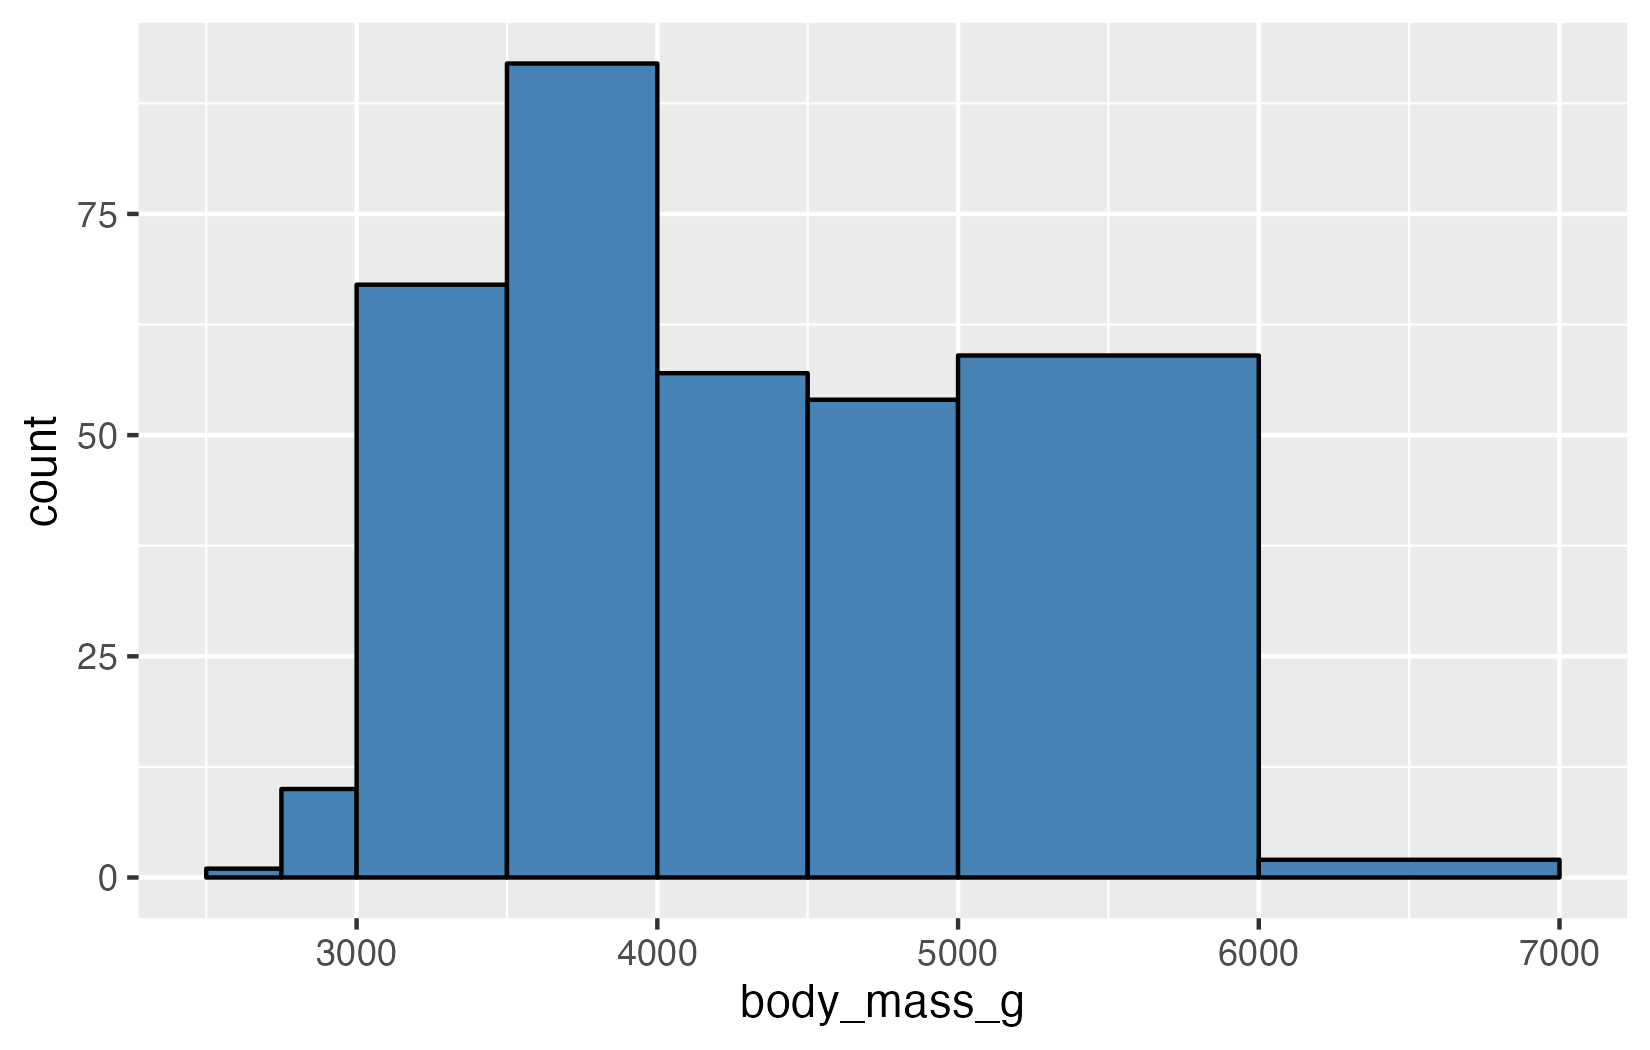
\includegraphics{./03-visualization_files/figure-pdf/unnamed-chunk-17-1.png}

}

\end{figure}

Vous constatez ici que les choix effectués ne sont pas très pertinents :
toutes les classes n'ont pas la même largeur. Cela rend l'interprétation
difficile. Il est donc vivement conseillé, pour spécifier
\texttt{breaks}, de créer des suites régulières, comme avec la fonction
\texttt{seq()} (consultez son fichier d'aide et les exemples) :

\begin{Shaded}
\begin{Highlighting}[]
\NormalTok{limites }\OtherTok{\textless{}{-}} \FunctionTok{seq}\NormalTok{(}\AttributeTok{from =} \DecValTok{2500}\NormalTok{, }\AttributeTok{to =} \DecValTok{6500}\NormalTok{, }\AttributeTok{by =} \DecValTok{250}\NormalTok{)}
\NormalTok{limites}
\end{Highlighting}
\end{Shaded}

\begin{verbatim}
 [1] 2500 2750 3000 3250 3500 3750 4000 4250 4500 4750 5000 5250 5500 5750 6000
[16] 6250 6500
\end{verbatim}

\begin{Shaded}
\begin{Highlighting}[]
\FunctionTok{ggplot}\NormalTok{(penguins, }\FunctionTok{aes}\NormalTok{(}\AttributeTok{x =}\NormalTok{ body\_mass\_g)) }\SpecialCharTok{+}
  \FunctionTok{geom\_histogram}\NormalTok{(}\AttributeTok{fill =} \StringTok{"steelblue"}\NormalTok{, }\AttributeTok{color =} \StringTok{"black"}\NormalTok{,}
                 \AttributeTok{breaks =}\NormalTok{ limites)}
\end{Highlighting}
\end{Shaded}

\begin{figure}[H]

{\centering 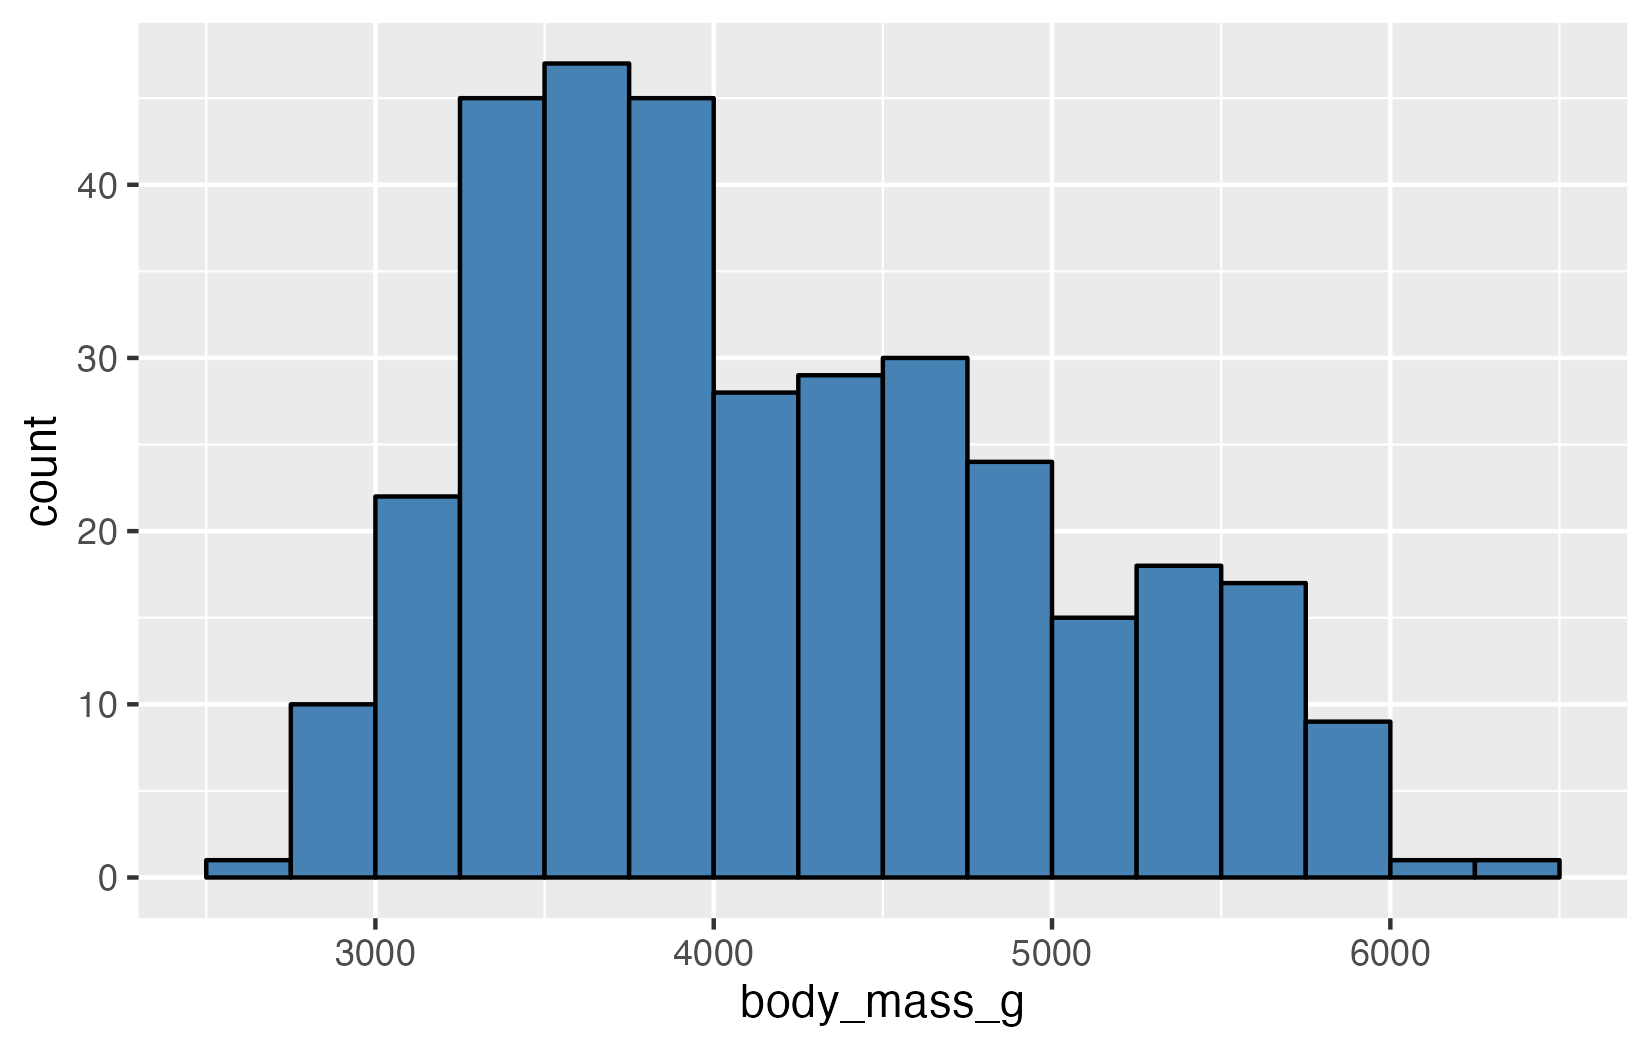
\includegraphics{./03-visualization_files/figure-pdf/unnamed-chunk-18-1.png}

}

\caption{Un exemple d'utilisation de l'argument \texttt{breaks}}

\end{figure}

Il est important que toute la gamme des valeurs de
\texttt{body\_mass\_g} soit bien couverte par les limites des classes
que nous avons définies, sinon, certaines valeurs sont omises et
l'histogramme est donc incomplet/incorrect. Une façon de s'en assurer
est d'afficher le résumé des données pour la colonne
\texttt{body\_mass\_g} du jeu de données \texttt{penguins} :

\begin{Shaded}
\begin{Highlighting}[]
\FunctionTok{summary}\NormalTok{(penguins}\SpecialCharTok{$}\NormalTok{body\_mass\_g)}
\end{Highlighting}
\end{Shaded}

\begin{verbatim}
   Min. 1st Qu.  Median    Mean 3rd Qu.    Max.    NA's 
   2700    3550    4050    4202    4750    6300       2 
\end{verbatim}

On voit ici que les masses varient de 2700 à 6300 grammes. Les classes
que nous avons définies couvrent une plage de masses plus large (de 2500
à 6500). Toutes les données sont donc bien intégrées à l'histogramme.

\hypertarget{geom_rug-et-geom_density}{%
\subsubsection{\texorpdfstring{\texttt{geom\_rug} et
\texttt{geom\_density}}{geom\_rug et geom\_density}}\label{geom_rug-et-geom_density}}

La fonction \texttt{geom\_histogram()} n'est pas la seule qui permette
de visualiser la distribution des données. Il est en effet possible
d'utiliser d'autres objets géométriques, en plus ou à la place de
\texttt{geom\_histogram()} pour ajouter de l'information sur le
graphique, ou pour visualiser différemment la distribution des mêmes
données.

La fonction \texttt{geom\_rug()} permet d'ajouter les données réelles
sous forme de segments, sous un histogramme. Cela prend souvent l'aspect
d'une sorte de tapis, d'où le nom de la fonction (``rug'' signifie
``tapis'' en anglais). Pour ajouter une couche supplémentaire au
graphique, on ajoute simplement un \texttt{+} à la fin de la dernière
ligne, et sur la ligne suivante, on ajoute un objet géométrique
supplémentaire :

\begin{Shaded}
\begin{Highlighting}[]
\FunctionTok{ggplot}\NormalTok{(penguins, }\FunctionTok{aes}\NormalTok{(}\AttributeTok{x =}\NormalTok{ body\_mass\_g)) }\SpecialCharTok{+}
  \FunctionTok{geom\_histogram}\NormalTok{(}\AttributeTok{fill =} \StringTok{"steelblue"}\NormalTok{, }\AttributeTok{color =} \StringTok{"black"}\NormalTok{,}
                 \AttributeTok{bins =} \DecValTok{25}\NormalTok{) }\SpecialCharTok{+}
  \FunctionTok{geom\_rug}\NormalTok{()}
\end{Highlighting}
\end{Shaded}

\begin{verbatim}
Warning: Removed 2 rows containing non-finite values (stat_bin).
\end{verbatim}

\begin{figure}[H]

{\centering 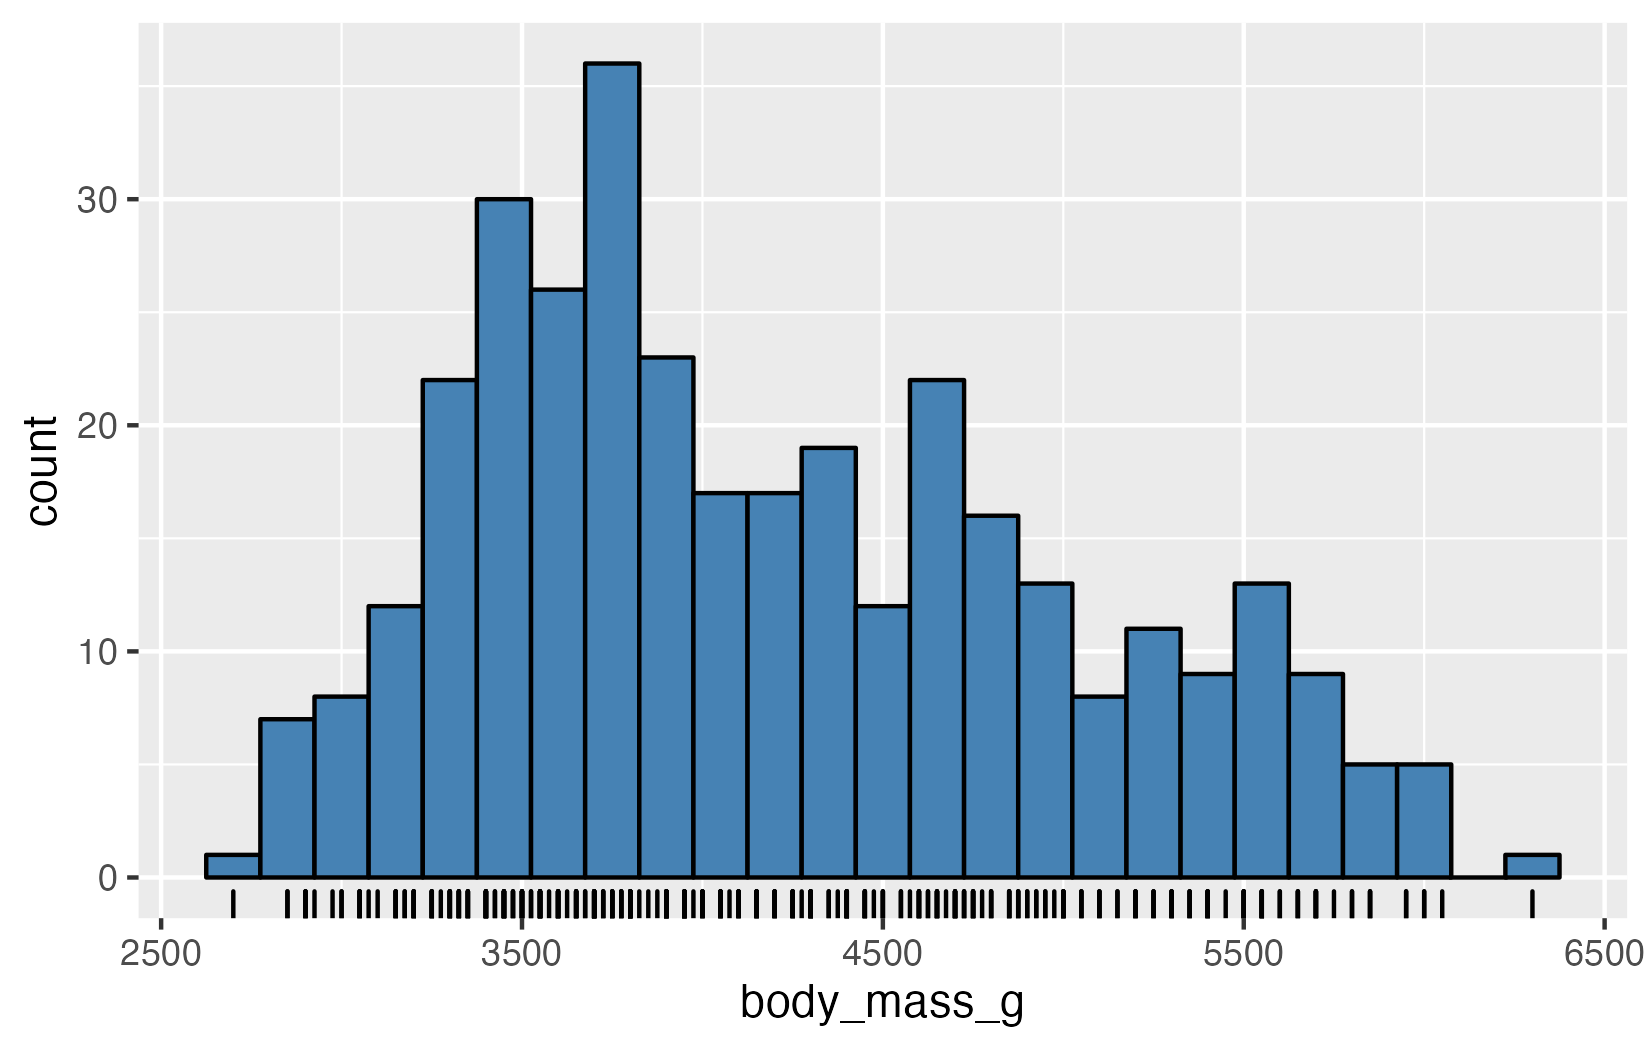
\includegraphics{./03-visualization_files/figure-pdf/unnamed-chunk-20-1.png}

}

\end{figure}

Les tirets qui sont maintenant visibles en-dessous de l'histogramme
correspondent aux 342 valeurs de masses réellement observées dans le jeu
de données. Puisque certaines tailles ont été observées plusieurs fois,
faire des tirets semi-transparents nous permettra de mieux visualiser
quelles tailles ont été observées fréquemment ou rarement. On peut
régler la transparence des éléments d'un graphique avec l'argument
\texttt{alpha\ =}, qui prend des valeurs comprises entre 0 (transparence
totale) et 1 (opacité totale) :

\begin{Shaded}
\begin{Highlighting}[]
\FunctionTok{ggplot}\NormalTok{(penguins, }\FunctionTok{aes}\NormalTok{(}\AttributeTok{x =}\NormalTok{ body\_mass\_g)) }\SpecialCharTok{+}
  \FunctionTok{geom\_histogram}\NormalTok{(}\AttributeTok{fill =} \StringTok{"steelblue"}\NormalTok{, }\AttributeTok{color =} \StringTok{"black"}\NormalTok{,}
                 \AttributeTok{bins =} \DecValTok{25}\NormalTok{) }\SpecialCharTok{+}
  \FunctionTok{geom\_rug}\NormalTok{(}\AttributeTok{alpha =} \FloatTok{0.3}\NormalTok{)}
\end{Highlighting}
\end{Shaded}

\begin{verbatim}
Warning: Removed 2 rows containing non-finite values (stat_bin).
\end{verbatim}

\begin{figure}[H]

{\centering 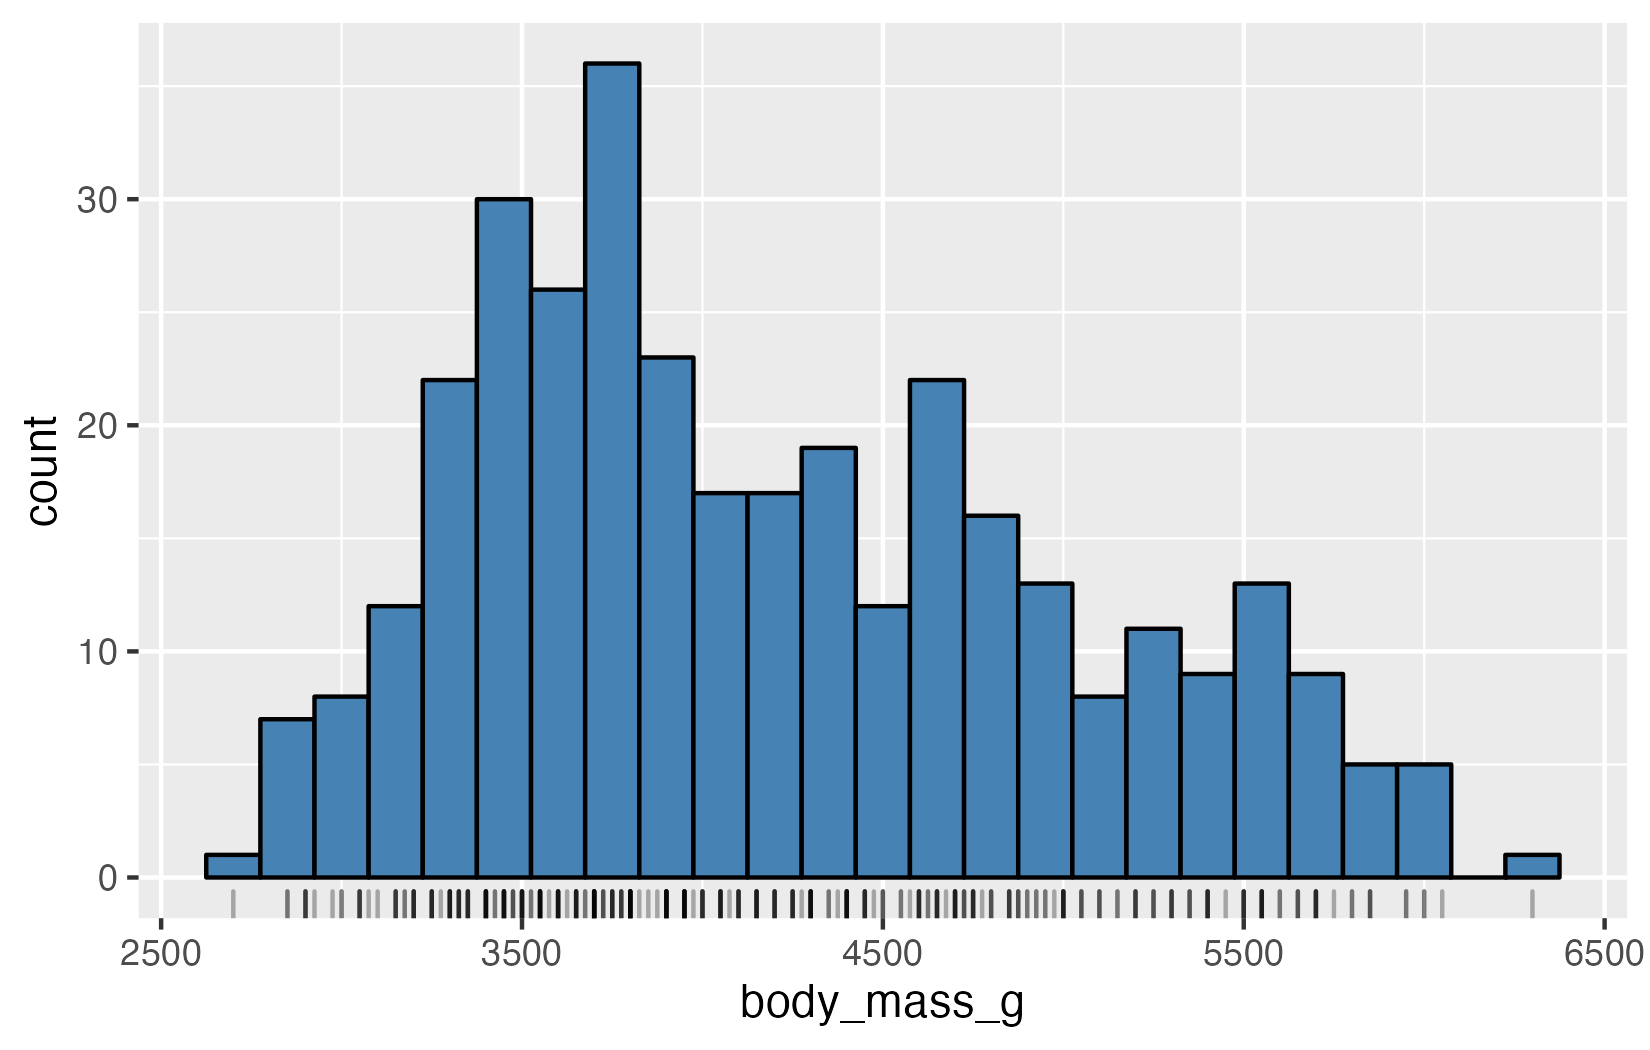
\includegraphics{./03-visualization_files/figure-pdf/unnamed-chunk-21-1.png}

}

\end{figure}

Les tirets sont maintenant d'autant plus foncés que les tailles ont été
observées un grand nombre de fois. On retrouve bien ici la distribution
décrite plus haut, avec 3 principaux groupes de valeurs. Cela révèle
certainement en partie la complexité des données : ces tailles
correspondent en effet aux mesures effectuées chez 3 espèces distinctes
qui peuvent avoir des caractéristiques différentes, sans compter que le
sexe des individus, qui n'apparaît pas ici, entre aussi probablement en
jeu. Nous y reviendrons plus tard.

La fonction \texttt{geom\_density()} permet de s'affranchir de la
question du nombre ou de la largeur des classes de taille :

\begin{Shaded}
\begin{Highlighting}[]
\FunctionTok{ggplot}\NormalTok{(penguins, }\FunctionTok{aes}\NormalTok{(}\AttributeTok{x =}\NormalTok{ body\_mass\_g)) }\SpecialCharTok{+}
  \FunctionTok{geom\_density}\NormalTok{(}\AttributeTok{fill =} \StringTok{"steelblue"}\NormalTok{, }\AttributeTok{color =} \StringTok{"black"}\NormalTok{, }\AttributeTok{alpha =} \FloatTok{0.7}\NormalTok{, }\AttributeTok{bw =} \DecValTok{300}\NormalTok{)}
\end{Highlighting}
\end{Shaded}

\begin{verbatim}
Warning: Removed 2 rows containing non-finite values (stat_density).
\end{verbatim}

\begin{figure}[H]

{\centering 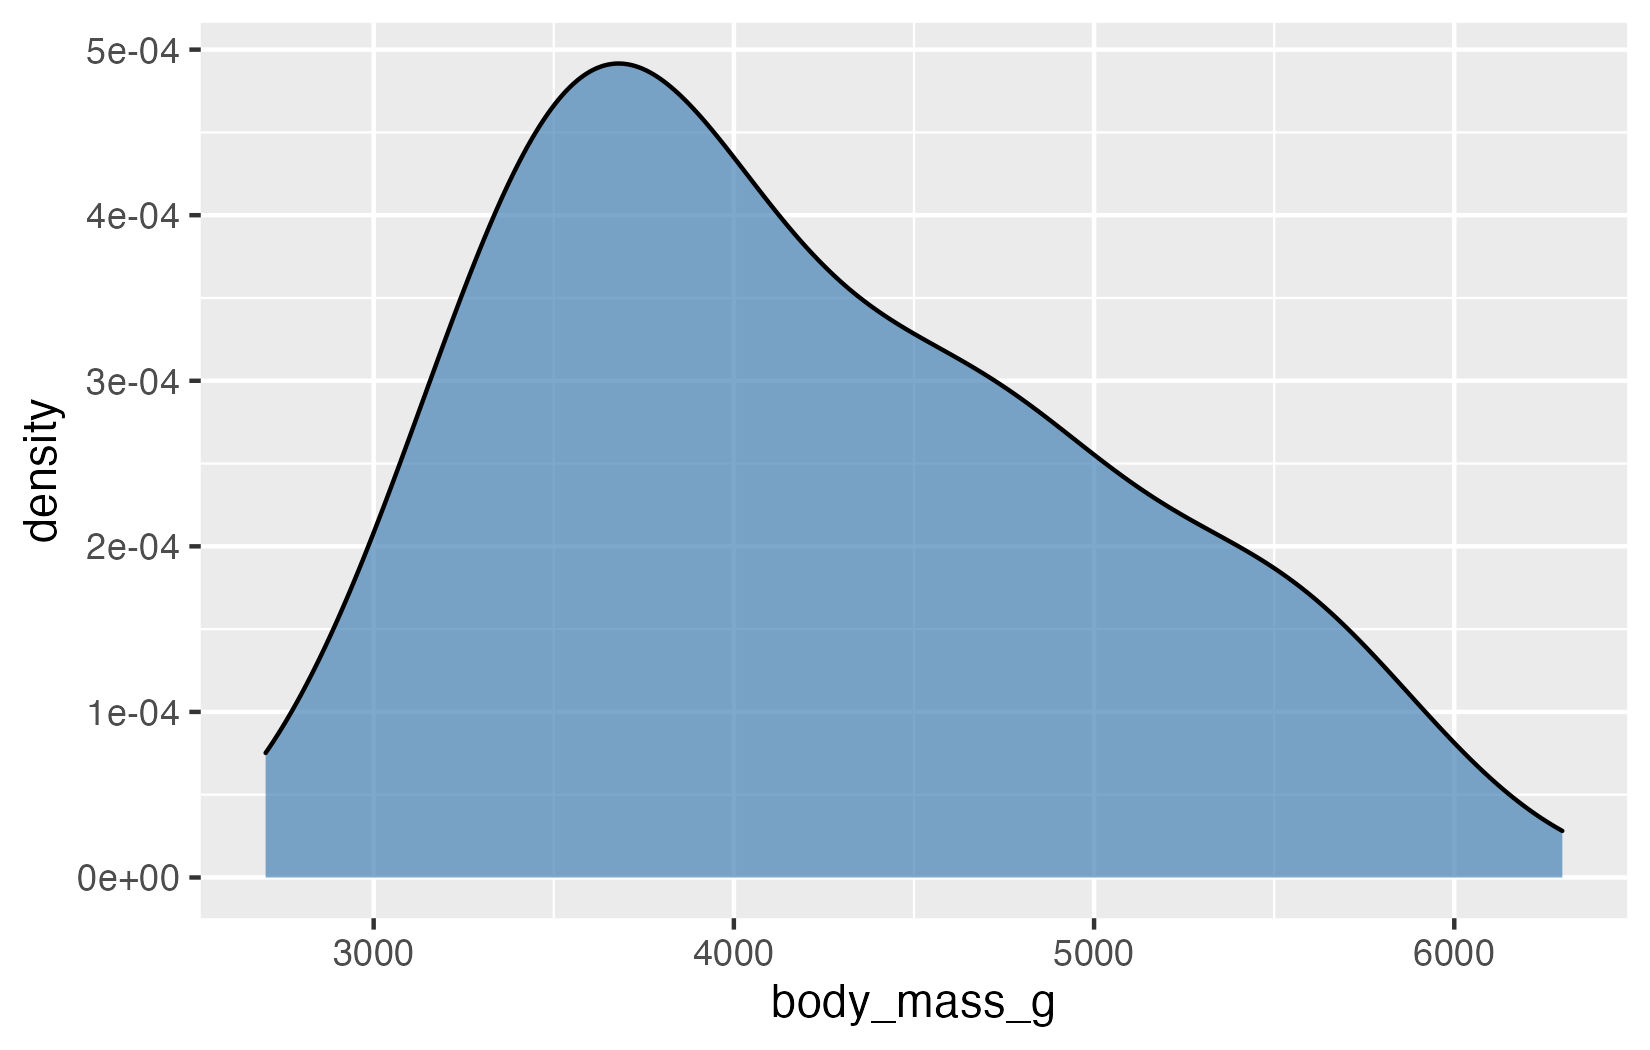
\includegraphics{./03-visualization_files/figure-pdf/unnamed-chunk-22-1.png}

}

\end{figure}

On obtient une sorte d'histogramme lissé qui fait bien apparaître les 3
tailles les plus fréquentes (au niveau des 3 ``bosses'' du graphique).
Inutile ici de spécifier un nombre de classes de taille, ou leur largeur
: le lissage est ici automatique. On peut modifier l'importance du
lissage avec l'argument \texttt{bw}, mais la valeur choisie par défaut
par \texttt{R} est généralement tout à fait satisfaisante. Vous pouvez
essayer avec une valeur de lissage de 30, puis de 500 pour vous rendre
compte de l'effet de ce paramètre.

Notez également que si l'histogramme présentait des valeurs d'abondance
sur l'axe des \texttt{y} (des nombres d'individus), le graphique de
densité présente, comme son nom l'indique, l'information de densité des
observations. Cela signifie que la surface totale sous la courbe (en
bleu) vaut 1. Cela peut s'avérer utile pour comparer plusieurs
distributions pour lesquelles on disposes de tailles d'échantillons très
différentes.

Enfin, on peut créer un graphique qui présentera à la fois l'histogramme
(avec \texttt{geom\_histogram()}), les données individuelles (avec
\texttt{geom\_rug()}) et la courbe de densité (avec
\texttt{geom\_density()}). Mais pour que tout s'affiche correctement, il
faut indiquer à \texttt{geom\_histogram} que l'axe des \texttt{y} doit
porter les densités et non les abondances. On fait cela en précisant
\texttt{y\ =\ ..density..}. Les deux points avant et après
\texttt{density} sont importants. Cela indique à \texttt{R} que la
variable \texttt{density} ne figure pas dans le tableau
\texttt{penguins}, mais qu'elle est calculée par la fonction
\texttt{geom\_histogram()} :

\begin{Shaded}
\begin{Highlighting}[]
\FunctionTok{ggplot}\NormalTok{(penguins, }\FunctionTok{aes}\NormalTok{(}\AttributeTok{x =}\NormalTok{ body\_mass\_g)) }\SpecialCharTok{+}
  \FunctionTok{geom\_histogram}\NormalTok{(}\FunctionTok{aes}\NormalTok{(}\AttributeTok{y =}\NormalTok{ ..density..),}
                 \AttributeTok{fill =} \StringTok{"steelblue"}\NormalTok{, }\AttributeTok{color =} \StringTok{"black"}\NormalTok{,}
                 \AttributeTok{bins =} \DecValTok{25}\NormalTok{, }\AttributeTok{alpha =} \FloatTok{0.7}\NormalTok{) }\SpecialCharTok{+}
  \FunctionTok{geom\_rug}\NormalTok{(}\AttributeTok{alpha =} \FloatTok{0.3}\NormalTok{) }\SpecialCharTok{+}
  \FunctionTok{geom\_density}\NormalTok{(}\AttributeTok{color =} \StringTok{"purple"}\NormalTok{, }\AttributeTok{size =} \DecValTok{2}\NormalTok{)}
\end{Highlighting}
\end{Shaded}

\begin{verbatim}
Warning: Removed 2 rows containing non-finite values (stat_bin).
\end{verbatim}

\begin{verbatim}
Warning: Removed 2 rows containing non-finite values (stat_density).
\end{verbatim}

\begin{figure}[H]

{\centering 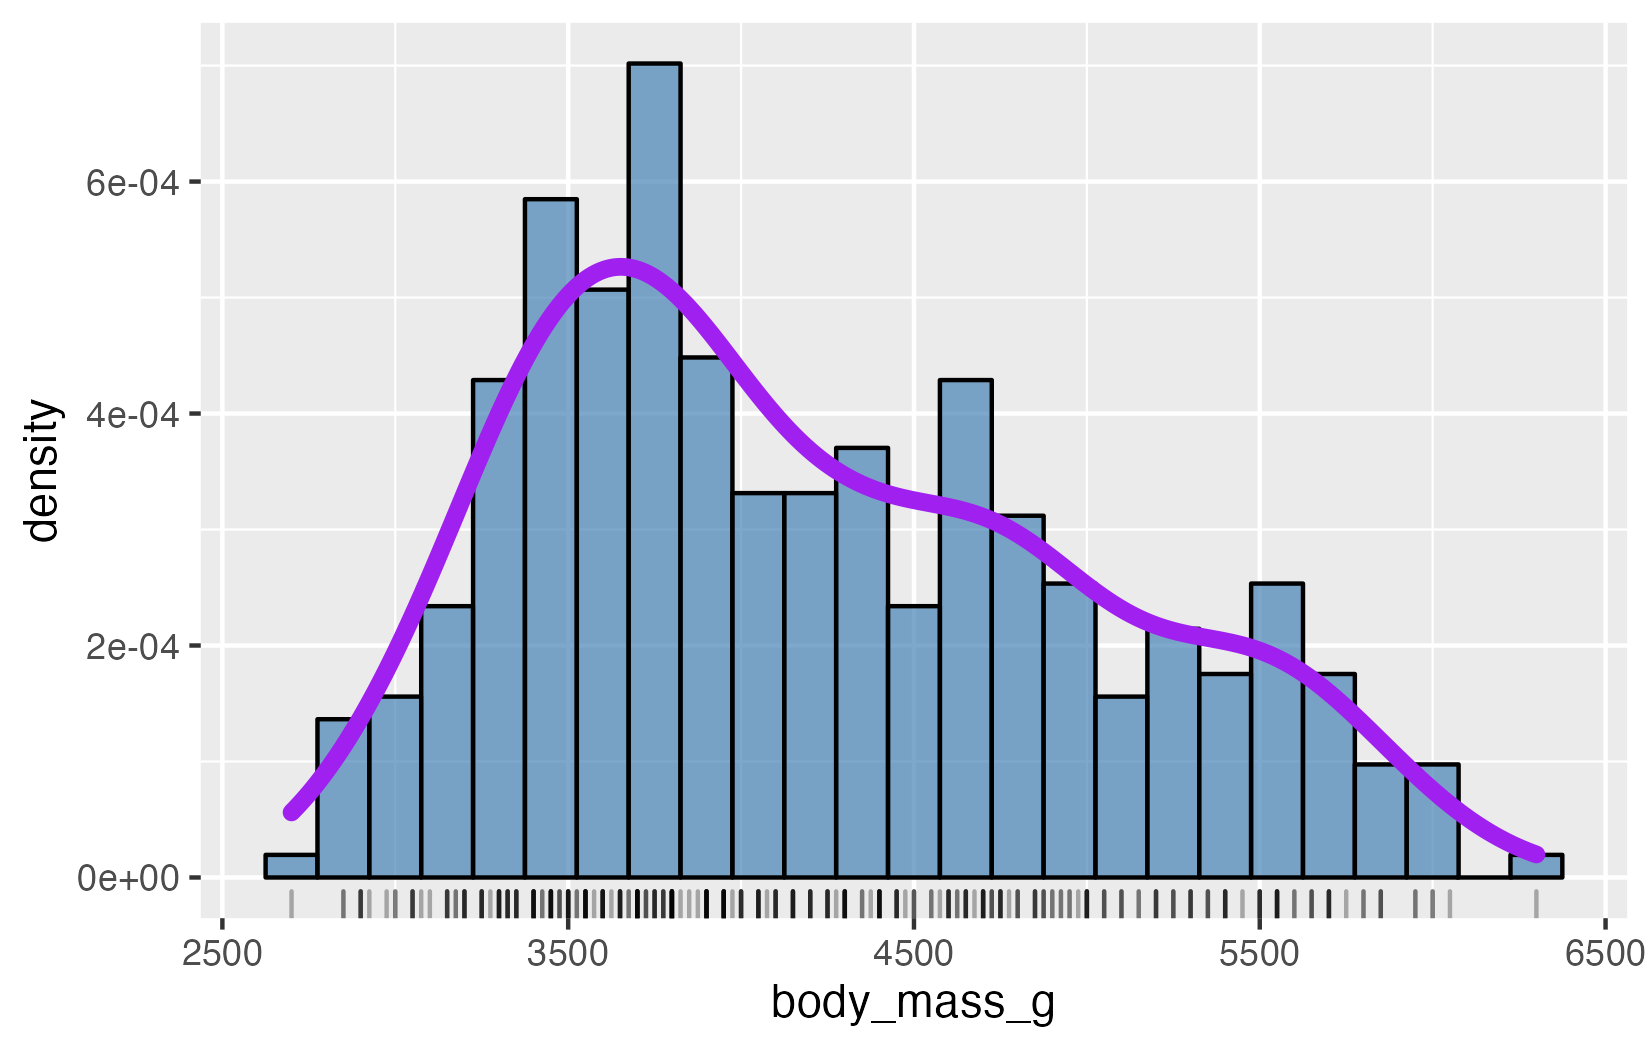
\includegraphics{./03-visualization_files/figure-pdf/unnamed-chunk-23-1.png}

}

\end{figure}

Notez l'utilisation des arguments \texttt{alpha}, \texttt{color} et
\texttt{size}, pour modifier l'aspect de différents éléments du
graphique. Assurez-vous d'avoir compris comment on les utilise, et
faites vos propres expériences.

\hypertarget{un-mot-sur-la-position-de-la-fonction-aes}{%
\subsubsection{\texorpdfstring{Un mot sur la position de la fonction
\texttt{aes()}}{Un mot sur la position de la fonction aes()}}\label{un-mot-sur-la-position-de-la-fonction-aes}}

Sur le dernier exemple, vous constatez que la fonction \texttt{aes()}
apparaît une fois à l'intérieur de la fonction \texttt{ggplot()}, et une
autre fois à l'intérieur de \texttt{geom\_histogram()}. Pourquoi ne pas
avoir tapé, plus simplement :

\begin{Shaded}
\begin{Highlighting}[]
\FunctionTok{ggplot}\NormalTok{(penguins, }\FunctionTok{aes}\NormalTok{(}\AttributeTok{x =}\NormalTok{ body\_mass\_g, }\AttributeTok{y =}\NormalTok{ ..density..)) }\SpecialCharTok{+}
  \FunctionTok{geom\_histogram}\NormalTok{(}\AttributeTok{fill =} \StringTok{"steelblue"}\NormalTok{, }\AttributeTok{color =} \StringTok{"black"}\NormalTok{,}
                 \AttributeTok{bins =} \DecValTok{25}\NormalTok{, }\AttributeTok{alpha =} \FloatTok{0.7}\NormalTok{) }\SpecialCharTok{+}
  \FunctionTok{geom\_rug}\NormalTok{(}\AttributeTok{alpha =} \FloatTok{0.3}\NormalTok{) }\SpecialCharTok{+}
  \FunctionTok{geom\_density}\NormalTok{(}\AttributeTok{color =} \StringTok{"purple"}\NormalTok{, }\AttributeTok{size =} \DecValTok{2}\NormalTok{)}
\end{Highlighting}
\end{Shaded}

L'explication est relativement simple, mais importante :

\begin{tcolorbox}[enhanced jigsaw, bottomtitle=1mm, title=\textcolor{quarto-callout-important-color}{\faExclamation}\hspace{0.5em}{Important}, breakable, opacitybacktitle=0.6, coltitle=black, opacityback=0, toprule=.15mm, toptitle=1mm, titlerule=0mm, colback=white, rightrule=.15mm, arc=.35mm, leftrule=.75mm, bottomrule=.15mm, left=2mm, colframe=quarto-callout-important-color-frame, colbacktitle=quarto-callout-important-color!10!white]
Ce qui est spécifié dans la fonction \texttt{ggplot()} s'applique à
toutes les couches du graphiques (donc ici, aux 3 couches
\texttt{geom\_histogram()}, \texttt{geom\_rug()} et
\texttt{geom\_density()}).

Ce qui est spécifié dans une fonction \texttt{geom\_...()} ne s'applique
qu'à cette couche géométrique particulière.
\end{tcolorbox}

Ainsi, ajouter \texttt{y\ =\ ..density..} à l'intérieur de
\texttt{ggplot()} renvoie donc un message d'erreur, car seule la
fonction \texttt{geom\_histogram()} calcule la variable
\texttt{..density..}, seule la fonction \texttt{geom\_histogram()} sait
quoi faire de cette variable. Dans notre exemple, il est en revanche
logique d'ajouter \texttt{aes(x\ =\ body\_mass\_g)} dans la fonction
\texttt{ggplot()}, car nos trois couches géométriques ont besoin de cet
argument, et pour les 3 couches géométriques, on associe bien cette
variable \texttt{body\_mass\_g} à l'axe des \texttt{x}. Toutefois, rien
ne nous empêche d'écrire ceci à la place :

\begin{Shaded}
\begin{Highlighting}[]
\FunctionTok{ggplot}\NormalTok{(}\AttributeTok{data =}\NormalTok{ penguins) }\SpecialCharTok{+}
  \FunctionTok{geom\_histogram}\NormalTok{(}\FunctionTok{aes}\NormalTok{(}\AttributeTok{x =}\NormalTok{ body\_mass\_g, }\AttributeTok{y =}\NormalTok{ ..density..),}
                 \AttributeTok{fill =} \StringTok{"steelblue"}\NormalTok{, }\AttributeTok{color =} \StringTok{"black"}\NormalTok{,}
                 \AttributeTok{bins =} \DecValTok{25}\NormalTok{, }\AttributeTok{alpha =} \FloatTok{0.7}\NormalTok{) }\SpecialCharTok{+}
  \FunctionTok{geom\_rug}\NormalTok{(}\FunctionTok{aes}\NormalTok{(}\AttributeTok{x =}\NormalTok{ body\_mass\_g),}
           \AttributeTok{alpha =} \FloatTok{0.3}\NormalTok{) }\SpecialCharTok{+}
  \FunctionTok{geom\_density}\NormalTok{(}\FunctionTok{aes}\NormalTok{(}\AttributeTok{x =}\NormalTok{ body\_mass\_g),}
               \AttributeTok{color =} \StringTok{"purple"}\NormalTok{, }\AttributeTok{size =} \DecValTok{2}\NormalTok{)}
\end{Highlighting}
\end{Shaded}

\begin{verbatim}
Warning: Removed 2 rows containing non-finite values (stat_bin).
\end{verbatim}

\begin{verbatim}
Warning: Removed 2 rows containing non-finite values (stat_density).
\end{verbatim}

\begin{figure}[H]

{\centering 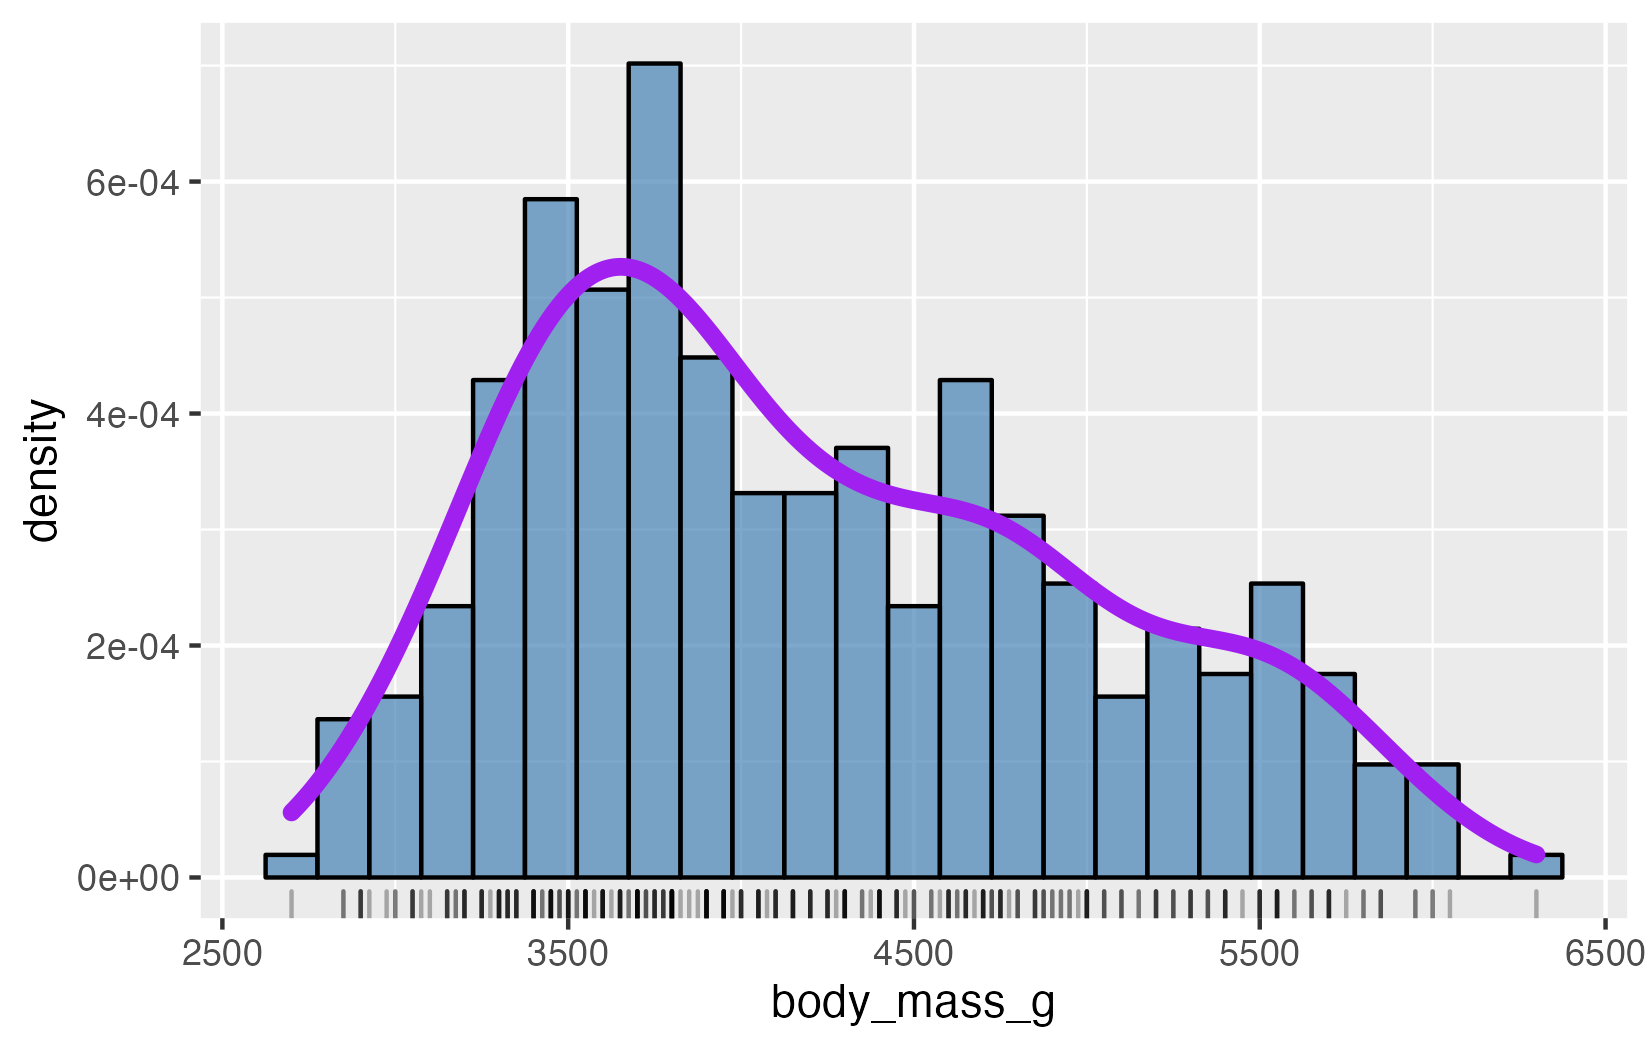
\includegraphics{./03-visualization_files/figure-pdf/unnamed-chunk-25-1.png}

}

\end{figure}

C'est plus long, mais c'est tout à fait correct et ça produit exactement
le même résultat qu'auparavant.

\hypertarget{sec-cloud}{%
\subsection{Les nuages de points et stripcharts}\label{sec-cloud}}

Pour ces deux types de graphiques, la variable numérique sera portée par
l'axe des \texttt{y}, et toutes les valeurs seront visibles, de façon
non agrégée (contrairement aux histogrammes où les valeurs individuelles
sont rassemblées à l'intérieur de classes). La différence entre les deux
types de graphiques tient à la nature des informations qui figureront
sur l'axe des \texttt{x} :

\begin{itemize}
\tightlist
\item
  Pour les nuages de points, l'axe des \texttt{x} portera simplement
  l'information du numéro d'observation pour chaque individu. L'individu
  placé sur la première ligne du tableau de données portera l'indice
  \texttt{1}. L'individu placé sur la deuxième ligne du tableau de
  données portera l'indice \texttt{2}, et ainsi de suite jusqu'à
  l'individu placé sur la dernière ligne du tableau (il portera ici
  l'indice 344 puisque le tableau compte 344 lignes)
\item
  Pour un stripchart, l'axe des \texttt{x} portera une unique valeur, la
  même pour tous les individus
\end{itemize}

Dans les deux cas, l'axe des \texttt{x} ne nous sera pas vraiment utile.
Il nous servira simplement à afficher des points sur un graphique, mais
puisque nous ne disposons que d'une unique variable, c'est bien l'axe
des \texttt{y} qui nous intéressera en priorité. Pour faire un nuage de
points, on utilise \texttt{geom\_point()}, et pour un stripchart
\texttt{geom\_jitter()}. Commençons par examiner le nuage de points pour
la variable \texttt{body-mass-g} :

\begin{Shaded}
\begin{Highlighting}[]
\FunctionTok{ggplot}\NormalTok{(penguins, }\FunctionTok{aes}\NormalTok{(}\AttributeTok{x =} \FunctionTok{seq\_along}\NormalTok{(body\_mass\_g), }\AttributeTok{y =}\NormalTok{ body\_mass\_g)) }\SpecialCharTok{+}
  \FunctionTok{geom\_point}\NormalTok{()}
\end{Highlighting}
\end{Shaded}

\begin{verbatim}
Warning: Removed 2 rows containing missing values (geom_point).
\end{verbatim}

\begin{figure}[H]

{\centering 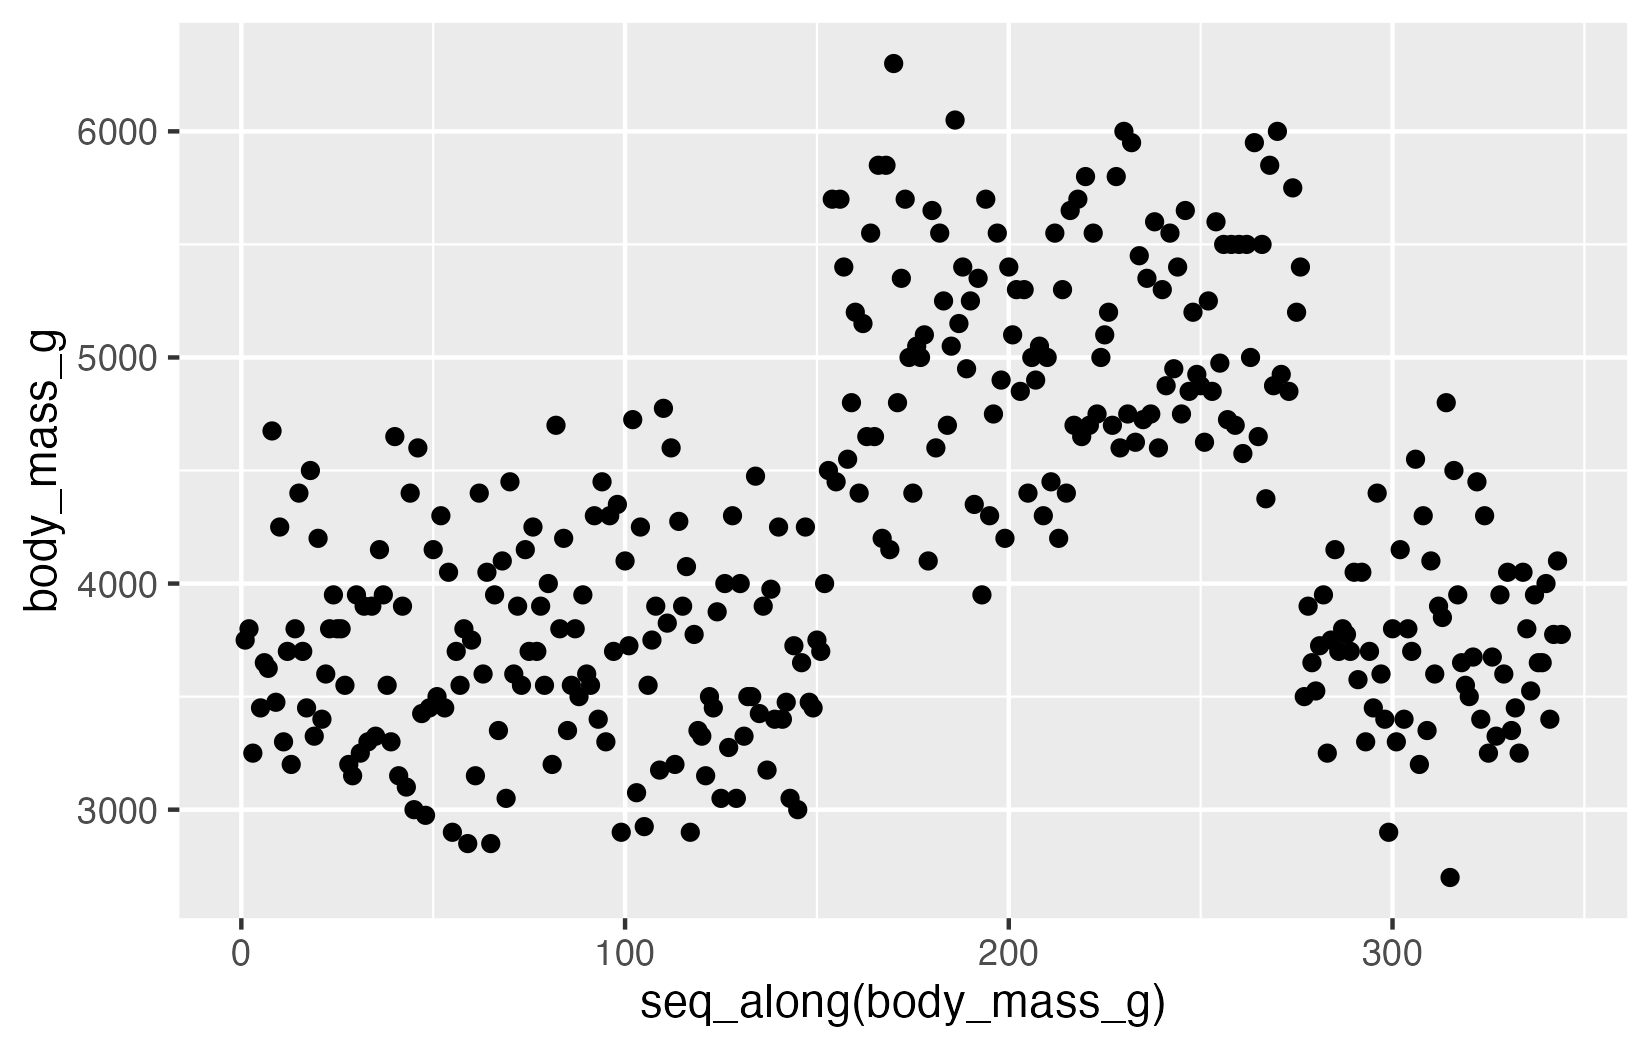
\includegraphics{./03-visualization_files/figure-pdf/unnamed-chunk-26-1.png}

}

\end{figure}

C'est la fonction \texttt{seq\_along()}, que l'on associe à l'axe des
\texttt{x}, qui permet de faire apparaître les numéros de lignes du
tableau \texttt{penguins}. On constate ici que 3 groupes de points sont
présents :

\begin{enumerate}
\def\labelenumi{\arabic{enumi}.}
\tightlist
\item
  Pour les lignes 1 à 150 (environ), un premier groupe de points
  présente des masses comprises entre 3000 et 4800 grammes environ.
\item
  Pour les lignes 151 à 275 (environ), un second groupes de points
  présente des masses comprises entre 4000 et plus de 6000 grammes.
\item
  Pour les lignes 276 à 344 (environ), un troisième groupe de points
  présente des valeurs similaires à celles du premier groupe.
\end{enumerate}

En examinant le tableau \texttt{penguins} de plus près, on se rend
compte que les 3 espèces de manchots sont présentées dans l'ordre.
Ainsi, ces 3 groupes correspondent à 3 espèces différentes. Pour le
visualiser, il suffit d'associer la variable \texttt{species} à la
couleur des points. Puisqu'on cherche à associer une variable du tableau
de données à une caractéristique esthétique d'un objet géométrique, on
renseigne \texttt{color\ =\ species} à l'intérieur de \texttt{aes()} :

\begin{Shaded}
\begin{Highlighting}[]
\FunctionTok{ggplot}\NormalTok{(penguins, }\FunctionTok{aes}\NormalTok{(}\AttributeTok{x =} \FunctionTok{seq\_along}\NormalTok{(body\_mass\_g), }\AttributeTok{y =}\NormalTok{ body\_mass\_g)) }\SpecialCharTok{+}
  \FunctionTok{geom\_point}\NormalTok{(}\FunctionTok{aes}\NormalTok{(}\AttributeTok{color =}\NormalTok{ species))}
\end{Highlighting}
\end{Shaded}

\begin{verbatim}
Warning: Removed 2 rows containing missing values (geom_point).
\end{verbatim}

\begin{figure}[H]

{\centering 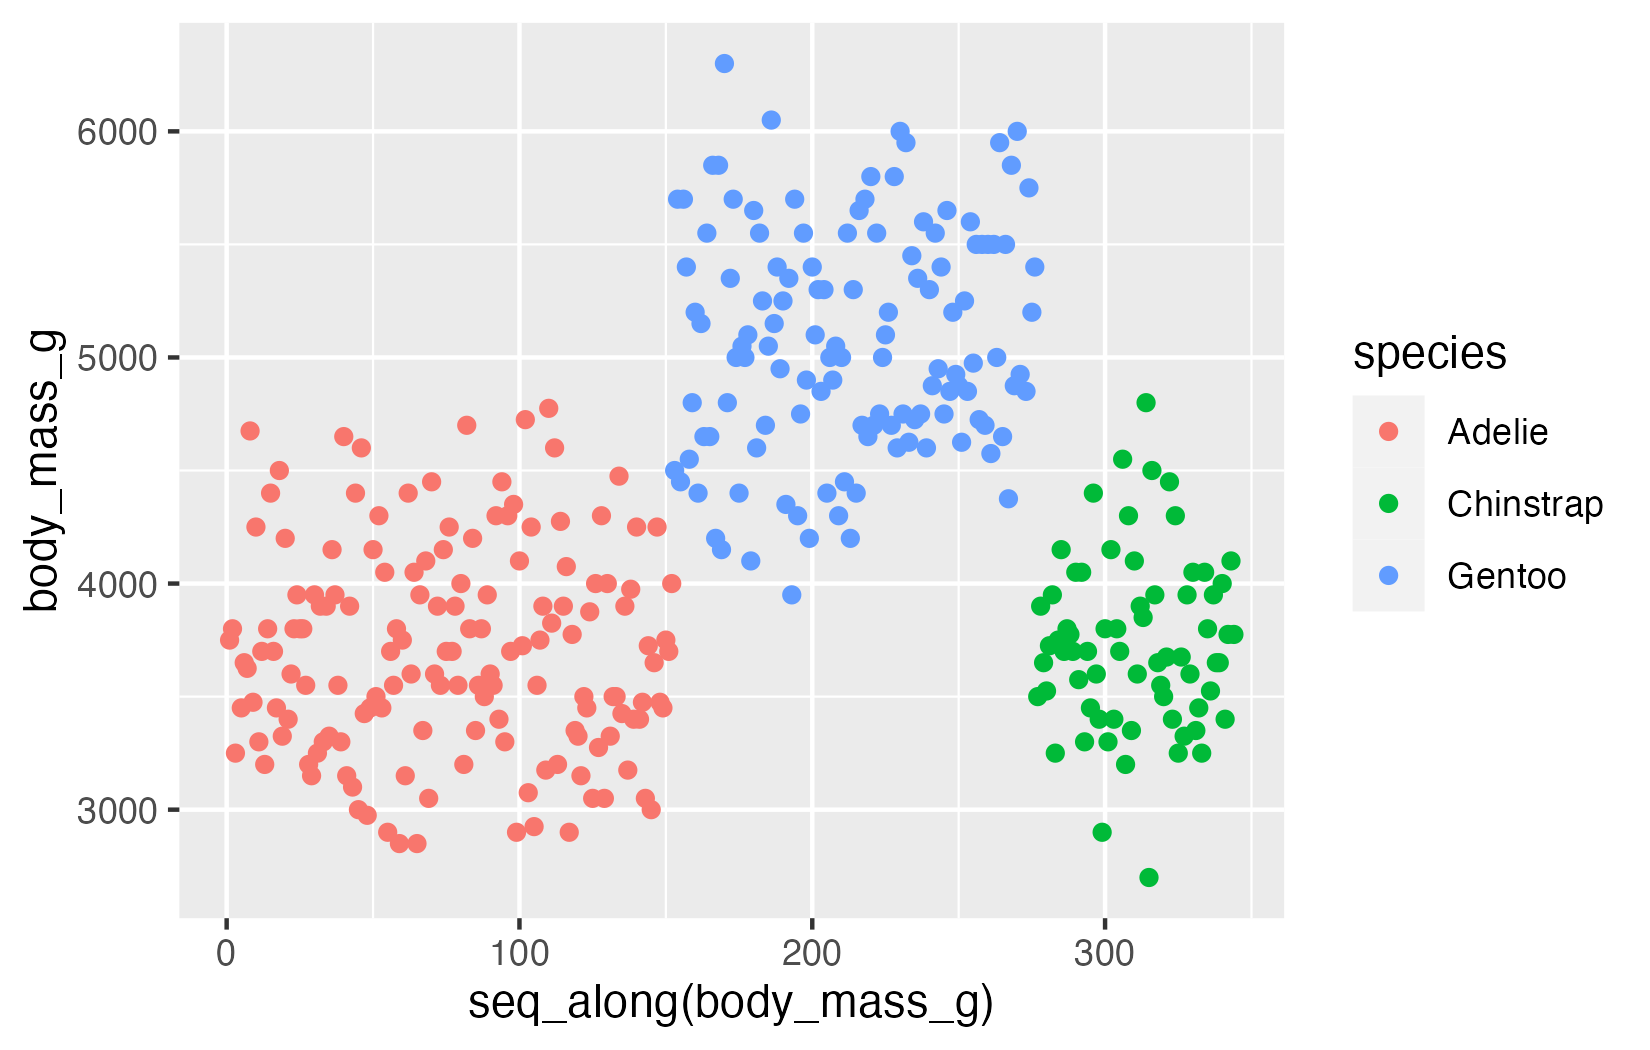
\includegraphics{./03-visualization_files/figure-pdf/fig-cloud-1.png}

}

\caption{\label{fig-cloud}Nuage de points des masses corporelles des 3
espèces de manchots}

\end{figure}

Attention, nous ne sommes déjà plus dans la situation d'une unique
variable numérique : nous avons ici visualisé 2 variables : une
numérique (portée par l'axe des \texttt{y}) et une catégorielle
(l'espèce représentée par la couleur des points). Ici, on constate que
les espèces Adélie et Chinstrap semblent avoir approximativement la même
gamme de masses, alors que les Gentoo semblent nettement plus lourds.

Comme pour les histogrammes, on peut utiliser des caractéristiques
esthétiques variées pour modifier l'apparence des points :

\begin{itemize}
\tightlist
\item
  \texttt{alpha} : la transparence. Choisir une valeur comprise entre 0
  (invisible) et 1 (totalement opaque)
\item
  \texttt{size} : la taille des points
\item
  \texttt{color} : la couleur des points (ou de leur contour pour les
  symboles qui permettent de spécifier une couleur de remplissage et une
  couleur de contour)
\item
  \texttt{fill} : la couleur de remplissage des points (pour les
  symboles qui permettent de spécifier une couleur de remplissage et une
  couleur de contour)
\item
  \texttt{shape} : pour modifier les symboles utilisés. Les symboles
  possibles sont codés ainsi :
\end{itemize}

\begin{figure}

{\centering 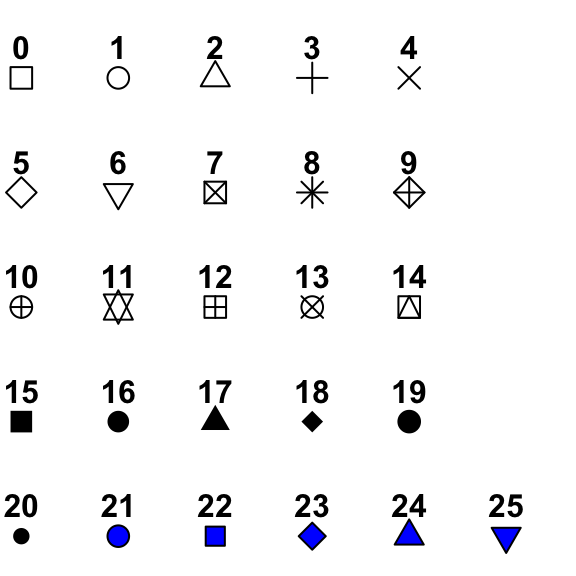
\includegraphics[width=0.5\textwidth,height=\textheight]{./images/pch.png}

}

\caption{\label{fig-pch}Liste des symboles et codes correspondants pour
les graphiques faisant apparaître des points. Pour les symboles 21 à 25,
il sera possible de spécifier une couleur de remplissage \texttt{fill}
et une couleur de contour \texttt{color}. Pour tous les autres symboles,
les changements de couleurs se feront avec l'argument \texttt{color}.}

\end{figure}

Chacune de ces caractéristiques esthétiques peut être associée à une
variable d'un tableau (il faut alors le spécifier à l'intérieur de
\texttt{aes()}), ou à une valeur unique, constante et identique pour
tous les points du graphique (il faut alors le spécifier à l'extérieur
de \texttt{aes()}). Par exemple :

\begin{Shaded}
\begin{Highlighting}[]
\FunctionTok{ggplot}\NormalTok{(penguins, }\FunctionTok{aes}\NormalTok{(}\AttributeTok{x =} \FunctionTok{seq\_along}\NormalTok{(body\_mass\_g), }\AttributeTok{y =}\NormalTok{ body\_mass\_g)) }\SpecialCharTok{+}
  \FunctionTok{geom\_point}\NormalTok{(}\AttributeTok{shape =} \DecValTok{23}\NormalTok{, }\AttributeTok{fill =} \StringTok{"steelblue"}\NormalTok{, }\AttributeTok{color =} \StringTok{"black"}\NormalTok{, }
             \AttributeTok{size =} \DecValTok{3}\NormalTok{, }\AttributeTok{alpha =} \FloatTok{0.5}\NormalTok{)}
\end{Highlighting}
\end{Shaded}

\begin{verbatim}
Warning: Removed 2 rows containing missing values (geom_point).
\end{verbatim}

\begin{figure}[H]

{\centering 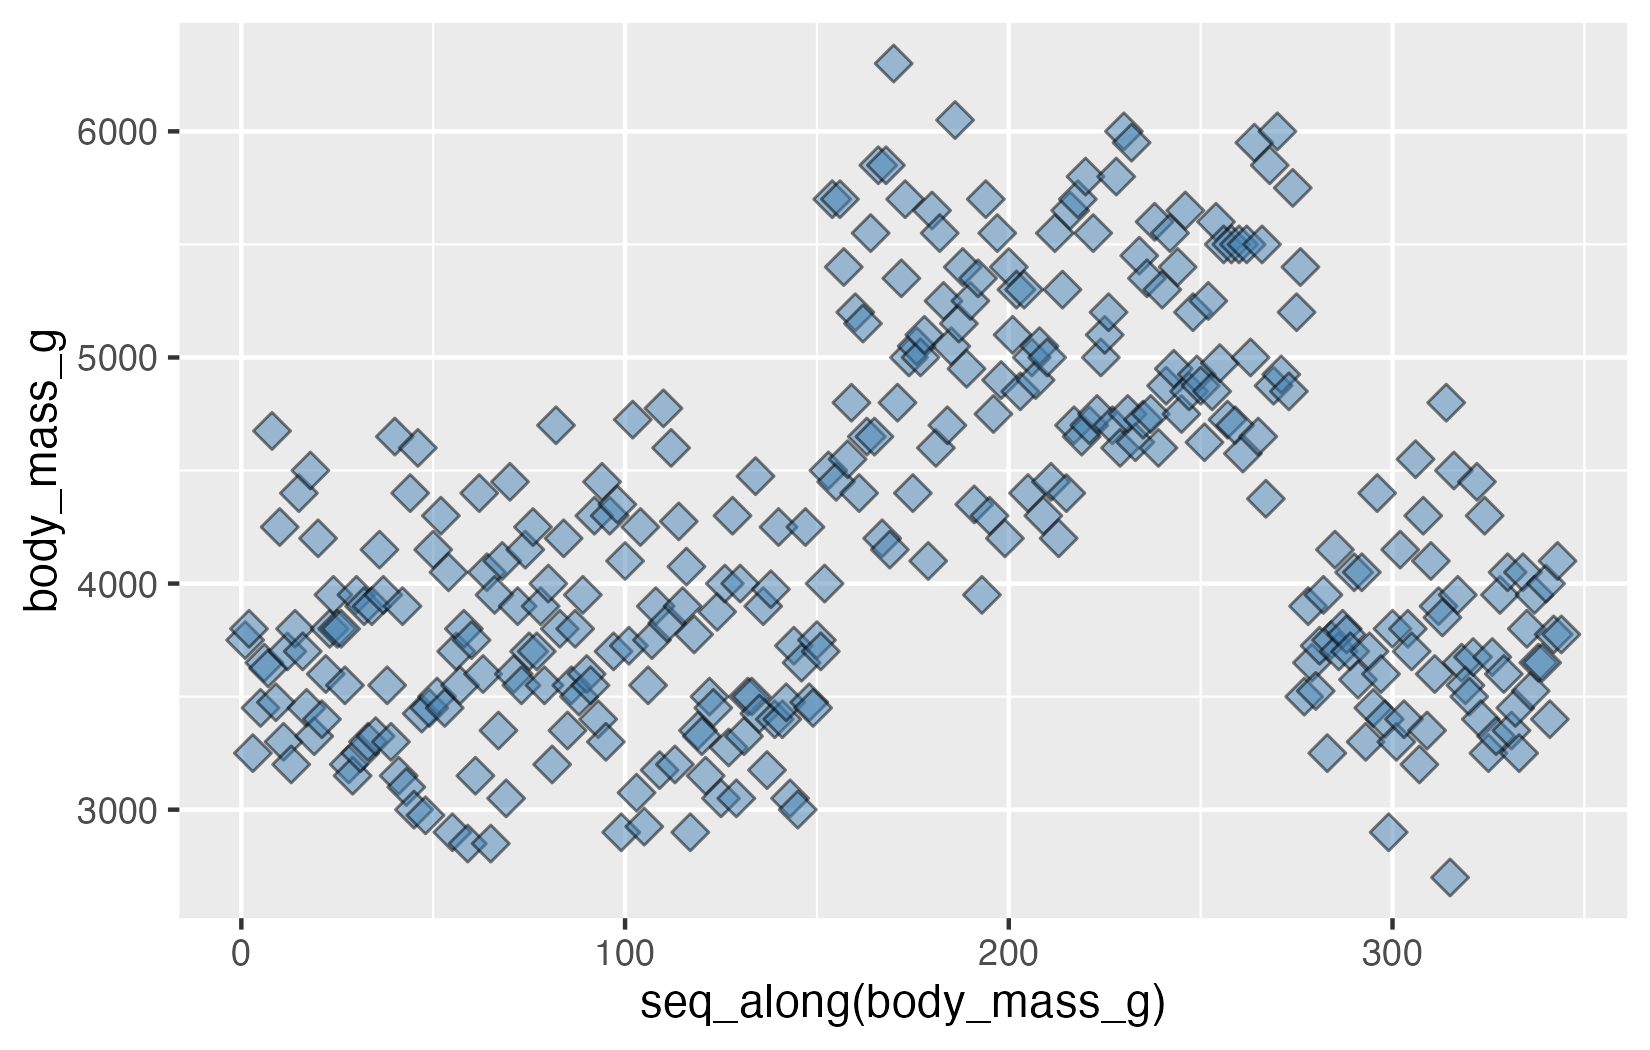
\includegraphics{./03-visualization_files/figure-pdf/unnamed-chunk-28-1.png}

}

\end{figure}

L'ajout de la transparence permet de régler le problème des points qui
se superposent (un phénomène nommé ``overplotting'').

Examinons à présent un exemple de stripchart :

\begin{Shaded}
\begin{Highlighting}[]
\FunctionTok{ggplot}\NormalTok{(penguins, }\FunctionTok{aes}\NormalTok{(}\AttributeTok{x =} \StringTok{""}\NormalTok{, }\AttributeTok{y =}\NormalTok{ body\_mass\_g)) }\SpecialCharTok{+}
  \FunctionTok{geom\_jitter}\NormalTok{()}
\end{Highlighting}
\end{Shaded}

\begin{verbatim}
Warning: Removed 2 rows containing missing values (geom_point).
\end{verbatim}

\begin{figure}[H]

{\centering 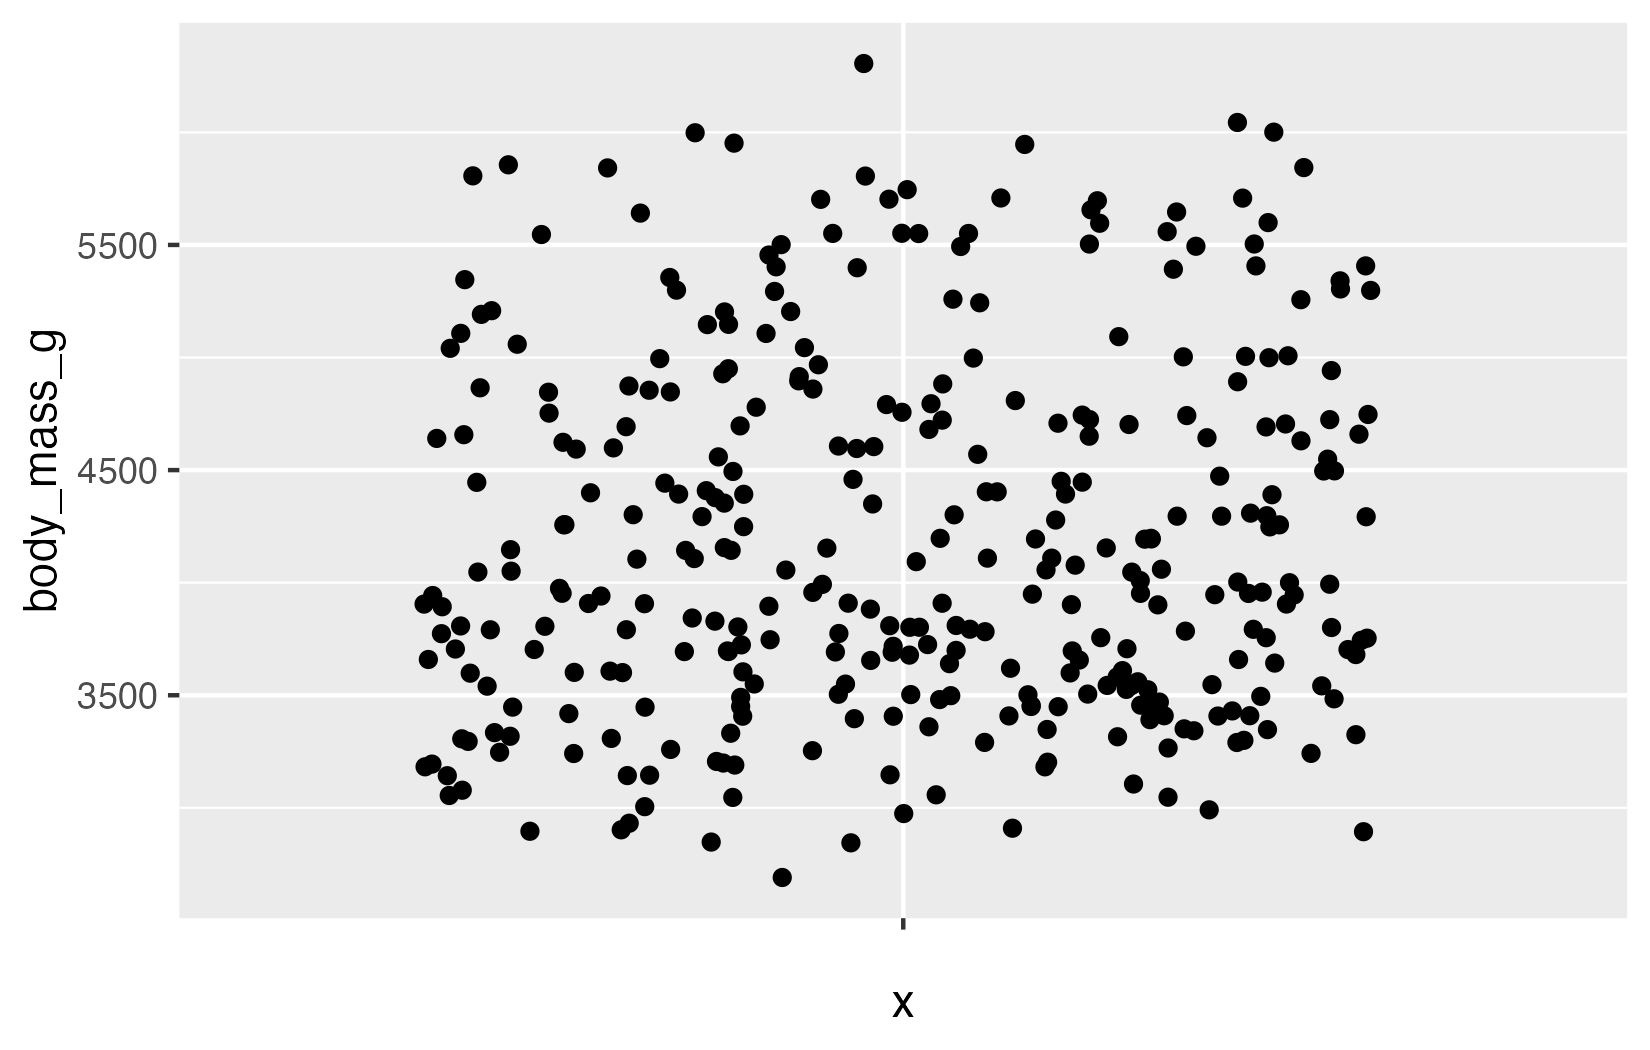
\includegraphics{./03-visualization_files/figure-pdf/unnamed-chunk-29-1.png}

}

\end{figure}

En indiquant \texttt{x\ =\ ""}, nous créons une unique catégorie pour
l'axe des abscisses, qui sera utilisée pour placer les valeurs de tous
les individus. Les valeurs de \texttt{body\_mass\_g} sont lues sur l'axe
des \texttt{y}, comme pour un nuage de point classique. Si les points
apparaissent dispersés, c'est en raison de 2 arguments spécifiques de la
fonction \texttt{geom\_jitter()} :

\begin{itemize}
\tightlist
\item
  \texttt{width\ =} permet de spécifier l'étendue horizontale du bruit
  aléatoire qui sera utilisé pour placer les points
\item
  \texttt{height\ =} permet de spécifier l'étendue verticale du bruit
  aléatoire qui sera utilisé pour placer les points
\end{itemize}

Si nous ne renseignons pas nous même ces deux arguments, ils sont fixés
automatiquement par le logiciel, ce qui n'est pas souhaitable, notamment
pour le bruit vertical. Pour mieux comprendre, voyons ce qui se passe
dans 3 situations :

\begin{Shaded}
\begin{Highlighting}[]
\FunctionTok{ggplot}\NormalTok{(penguins, }\FunctionTok{aes}\NormalTok{(}\AttributeTok{x =} \StringTok{""}\NormalTok{, }\AttributeTok{y =}\NormalTok{ body\_mass\_g)) }\SpecialCharTok{+}
  \FunctionTok{geom\_jitter}\NormalTok{(}\AttributeTok{width =} \DecValTok{0}\NormalTok{, }\AttributeTok{height =} \DecValTok{0}\NormalTok{)}

\FunctionTok{ggplot}\NormalTok{(penguins, }\FunctionTok{aes}\NormalTok{(}\AttributeTok{x =} \StringTok{""}\NormalTok{, }\AttributeTok{y =}\NormalTok{ body\_mass\_g)) }\SpecialCharTok{+}
  \FunctionTok{geom\_jitter}\NormalTok{(}\AttributeTok{width =} \FloatTok{0.1}\NormalTok{, }\AttributeTok{height =} \DecValTok{0}\NormalTok{)}

\FunctionTok{ggplot}\NormalTok{(penguins, }\FunctionTok{aes}\NormalTok{(}\AttributeTok{x =} \StringTok{""}\NormalTok{, }\AttributeTok{y =}\NormalTok{ body\_mass\_g)) }\SpecialCharTok{+}
  \FunctionTok{geom\_jitter}\NormalTok{(}\AttributeTok{width =} \FloatTok{0.1}\NormalTok{, }\AttributeTok{height =} \DecValTok{2000}\NormalTok{)}
\end{Highlighting}
\end{Shaded}

\begin{figure}

\begin{minipage}[t]{0.33\linewidth}

{\centering 

\raisebox{-\height}{

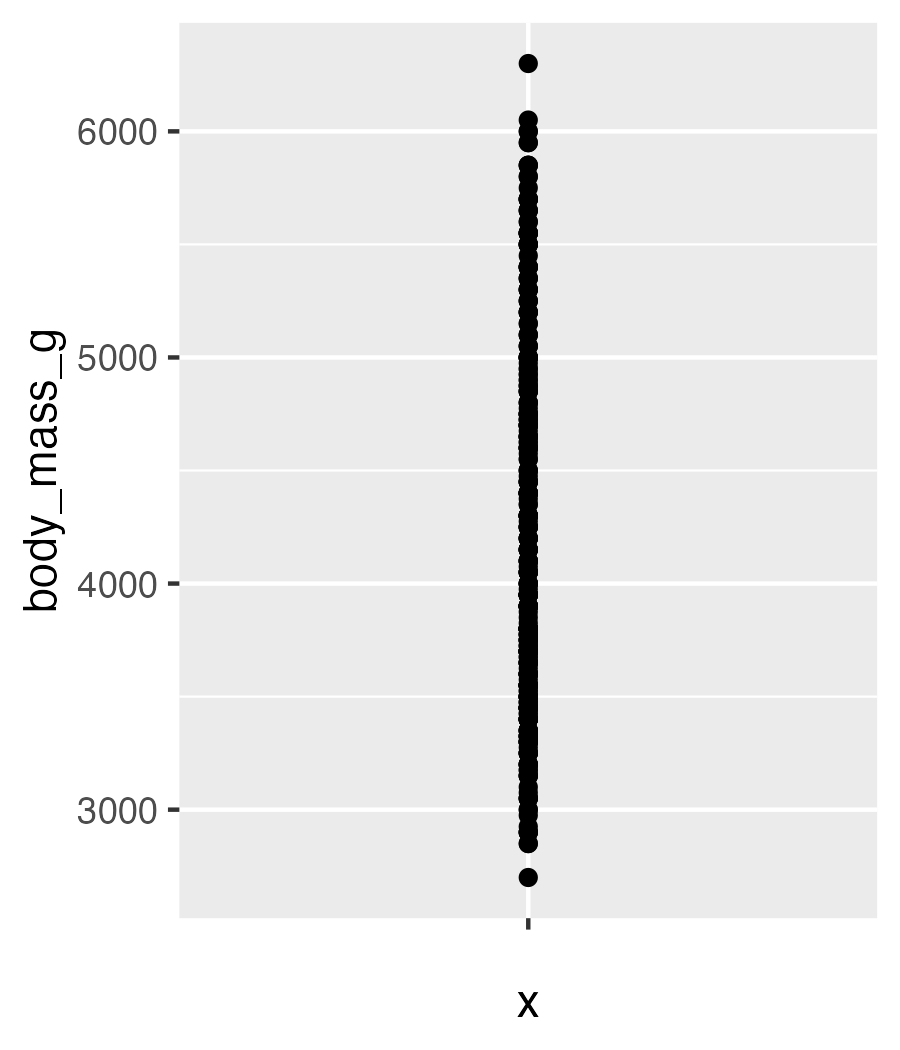
\includegraphics{./03-visualization_files/figure-pdf/fig-jitter-1.png}

}

}

\subcaption{\label{fig-jitter-1}Pas de dispersion horizontale, pas de
dispersion verticale}
\end{minipage}%
%
\begin{minipage}[t]{0.33\linewidth}

{\centering 

\raisebox{-\height}{

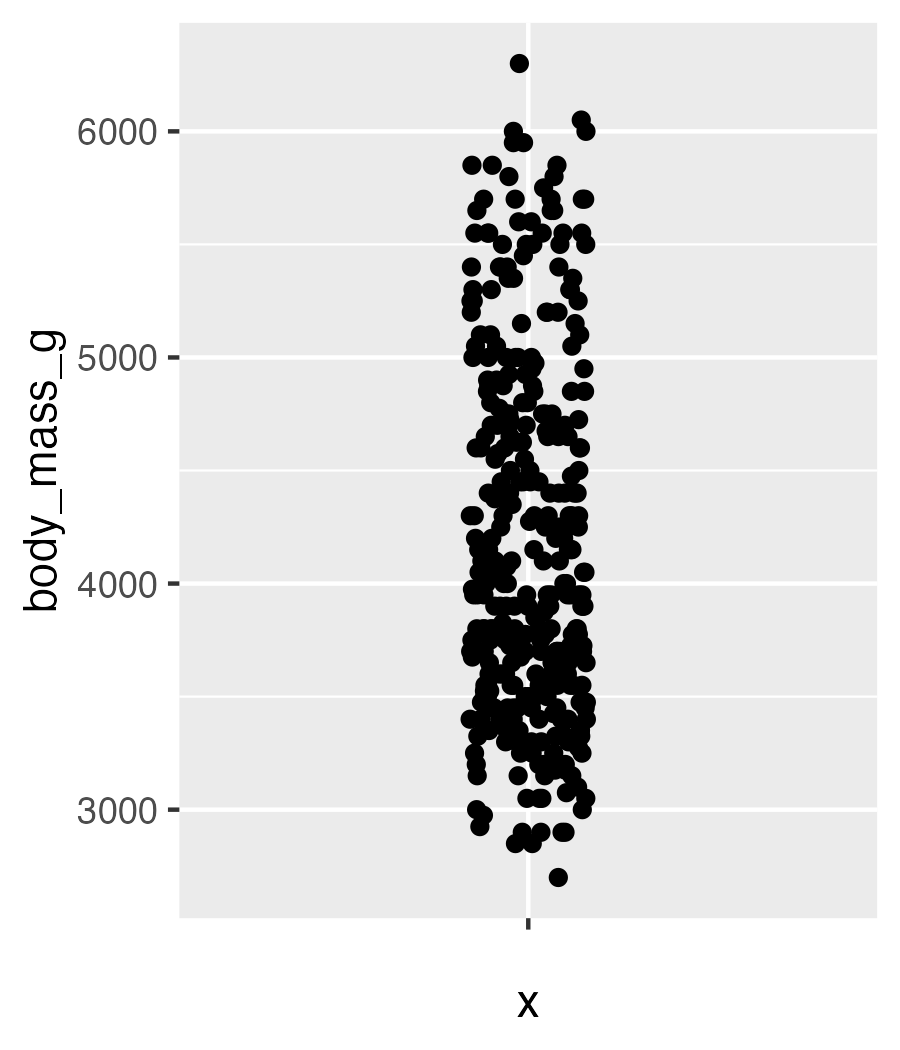
\includegraphics{./03-visualization_files/figure-pdf/fig-jitter-2.png}

}

}

\subcaption{\label{fig-jitter-2}Faible dispersion horizontale, pas de
dispersion verticale}
\end{minipage}%
%
\begin{minipage}[t]{0.33\linewidth}

{\centering 

\raisebox{-\height}{

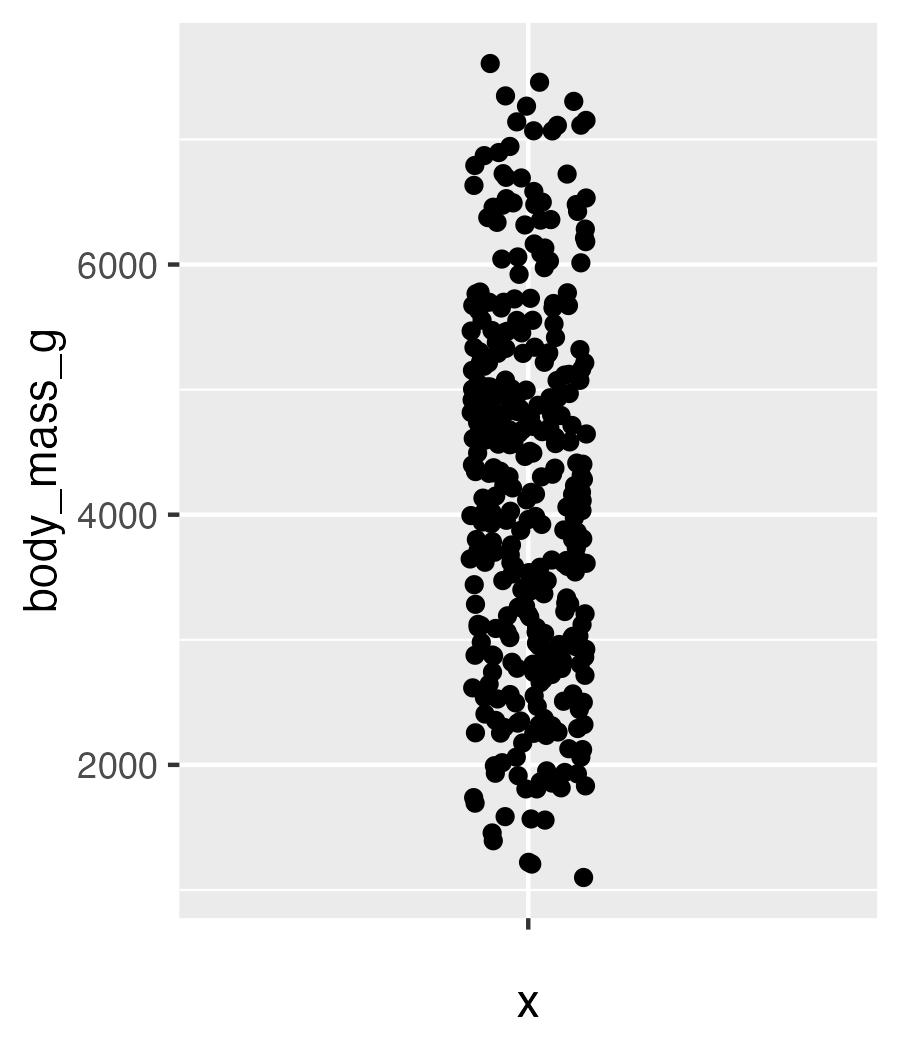
\includegraphics{./03-visualization_files/figure-pdf/fig-jitter-3.png}

}

}

\subcaption{\label{fig-jitter-3}Faible dispersion horizontale, forte
dispersion verticale}
\end{minipage}%

\caption{\label{fig-jitter}Trois exemples de stripchart}

\end{figure}

\begin{itemize}
\item
  Le premier exemple (sous-figure a) ne présente aucune dispersion, ni
  horizontale \texttt{width\ =\ 0}, \texttt{height\ =\ 0}. Les points
  apparaissent donc tous alignés, ils ont en effet tous la même valeur
  sur l'axe des abscisses. Leur position sur l'axe des \texttt{y}
  reflète la masse réellement observée pour chaque individu. Cette façon
  de représenter les données n'est pas très utile car la superposition
  des points vient empêcher la visualisation correcte de la distribution
  : ici, il est impossible de dire quelles sont les masses les plus
  fréquentes ou les plus rares.
\item
  Le second exemple (sous-figure b) présente une dispersion horizontale
  modérée \texttt{width\ =\ 0.1} et pas de dispersion verticale
  \texttt{height\ =\ 0}. Ici, tous les points ne sont plus alignés sur
  une seule droite. Puisque nous avons fixé \texttt{width\ =\ 0.1}, la
  position horizontale des points est choisie aléatoirement par
  \texttt{R} : il ajoute un léger bruit horizontale aléatoire, soit
  positif, soit négatif, avant de placer les points le long de l'axe des
  abscisses. Plus la valeur de \texttt{width} sera élevée, plus
  l'étendue du bruit horizontal sera importante. Sur l'axe des
  \texttt{y} en revanche, aucun bruit n'a été ajouté
  (\texttt{height\ =\ 0}). La position des points le long de cet axe
  reflète donc parfaitement la masse de chaque individu telle
  qu'enregistrées dans le tableau \texttt{penguins}. D'ailleurs, on
  constate que l'axe des ordonnées est strictement identique (même
  étendue, même graduations\ldots) pour les 2 premiers sous-graphiques.
  C'est ce type de représentation que nous recherchons. En effet,
  l'absence de bruit vertical nous permet de visualiser correctement
  (donc sans distorsion) la variable numérique choisie (ici
  \texttt{body\_mass\_g}), et le bruit horizontal nous permet d'étaler
  légèrement les points de part et d'autres d'un axe horizontal virtuel,
  ce qui a pour effet de réduire l'overplotting, et ce qui nous permet
  donc de visualiser les zones où les points sont plus nombreux/denses
  et les zones où les observations sont plus rares. Ici, on observe une
  majorité de points entre 3000 et 4000 grammes, une densité de points
  intermédiaire entre 4000 et 5000 grammes, et des points moins nombreux
  (donc moins d'individus) pour les masses supérieures à 5000 grammes.
\item
  Le troisième exemple (sous-figure c) présente une dispersion
  horizontale modérée \texttt{width\ =\ 0.1} et une importante
  dispersion verticale \texttt{height\ =\ 2000}. Cela signifie que la
  position des points sur l'axe des \texttt{y} ne reflète plus les
  vraies valeurs de masses enregistrées dans le tableau
  \texttt{penguins}, mais des valeurs de masses auxquelles un bruit
  aléatoire a été ajouté ou retiré. C'est ce qui explique que l'axe des
  ordonnées ne présente pas la même échelle que pour les 2 autres
  graphiques. Ce n'est évidemment pas souhaitable, car si nous voulons
  bel et bien ajouter un bruit horizontal pour éviter la superposition
  des points, il est essentiel de ne pas modifier la position verticale
  des points qui nous renseigne sur la variable d'intérêt. Ici, la
  troisième figure présente un axe des \texttt{y} différent des 2 autres
  figures, et la position verticale des points a été tellement altérée
  qu'on ne peut plus distinguer la sur-abondance de données entre 3000
  et 4000 grammes, ni la sous-représentation des observations au-dessus
  de 5000 grammes. Il sera donc important à l'avenir de toujours fixer
  \texttt{height\ =\ 0} pour faire un stripchart correct.
\end{itemize}

\begin{tcolorbox}[enhanced jigsaw, bottomtitle=1mm, title=\textcolor{quarto-callout-important-color}{\faExclamation}\hspace{0.5em}{Important}, breakable, opacitybacktitle=0.6, coltitle=black, opacityback=0, toprule=.15mm, toptitle=1mm, titlerule=0mm, colback=white, rightrule=.15mm, arc=.35mm, leftrule=.75mm, bottomrule=.15mm, left=2mm, colframe=quarto-callout-important-color-frame, colbacktitle=quarto-callout-important-color!10!white]

Sur un stripchart :

\begin{itemize}
\tightlist
\item
  la position \textbf{verticale} des points ne doit jamais être
  modifiée. On fixera donc toujours \texttt{height\ =\ 0}
\item
  la position \textbf{horizontale} des points doit être modifiée afin
  d'éviter l'overplotting et de visualiser les zones de fortes et
  faibles densités de points. On choisira donc en général des valeurs de
  \texttt{width} comprises entre \texttt{0.1} et \texttt{0.4}
\end{itemize}

\end{tcolorbox}

Enfin, puisqu'un stripchart permet d'afficher des points sur un
graphiques, les arguments permettant de modifier l'aspect des points
sont les mêmes que pour les nuages de points. Par exemple :

\begin{Shaded}
\begin{Highlighting}[]
\FunctionTok{ggplot}\NormalTok{(penguins, }\FunctionTok{aes}\NormalTok{(}\AttributeTok{x =} \StringTok{""}\NormalTok{, }\AttributeTok{y =}\NormalTok{ body\_mass\_g)) }\SpecialCharTok{+}
  \FunctionTok{geom\_jitter}\NormalTok{(}\FunctionTok{aes}\NormalTok{(}\AttributeTok{color =}\NormalTok{ species, }\AttributeTok{shape =}\NormalTok{ species),}
              \AttributeTok{size =} \DecValTok{3}\NormalTok{, }\AttributeTok{alpha =} \FloatTok{0.6}\NormalTok{, }
              \AttributeTok{width =} \FloatTok{0.1}\NormalTok{, }\AttributeTok{height =} \DecValTok{0}\NormalTok{)}
\end{Highlighting}
\end{Shaded}

\begin{verbatim}
Warning: Removed 2 rows containing missing values (geom_point).
\end{verbatim}

\begin{figure}[H]

{\centering 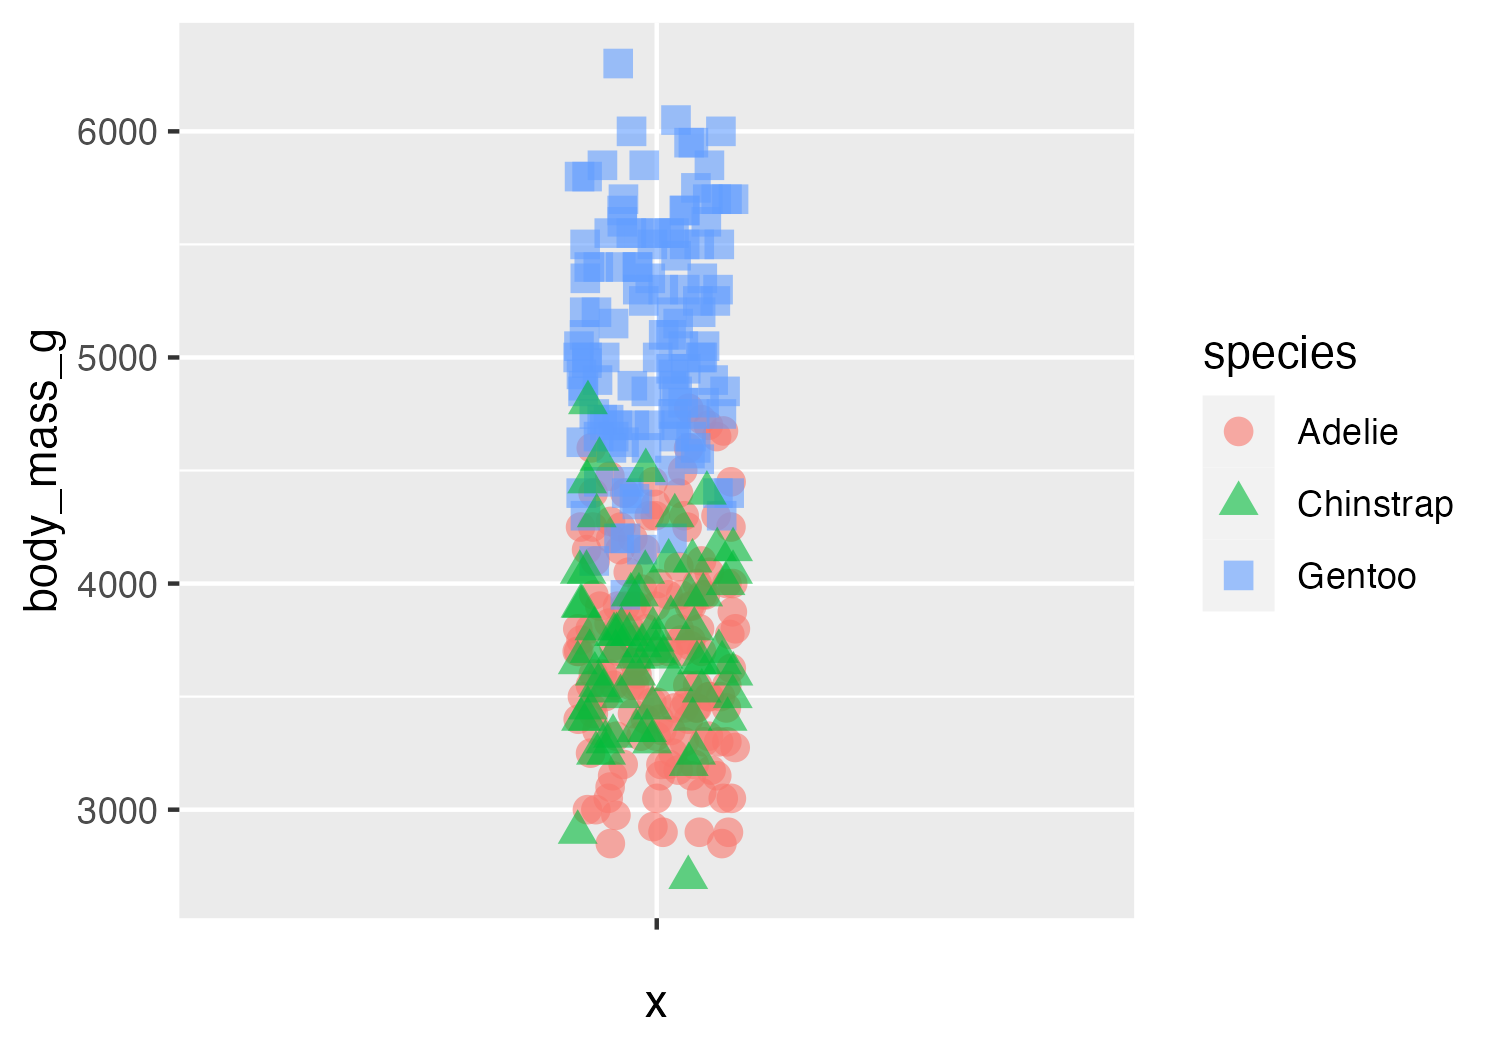
\includegraphics{./03-visualization_files/figure-pdf/fig-strip-1.png}

}

\caption{\label{fig-strip}Un exemple de stripchart}

\end{figure}

Sur cette figure, comme pour le nuage de points réalisé plus haut, j'ai
associé la variable \texttt{species} à la couleur des points (donc à
l'intérieur de \texttt{aes()}). J'ai également associé cette variable à
la forme des points \texttt{shape\ =\ species} à l'intérieur de
\texttt{aes()}. C'est ce qui explique que chacune des 3 espèces apparaît
sous la forme de symboles de formes et de couleurs différents. Pour
limiter l'overplotting, j'ai spécifié un bruit horizontal, et j'ai fixé
le bruit vertical à zéro. Enfin j'ai augmenté la taille des symboles
(avec \texttt{size\ =\ 3}, en dehors de \texttt{aes()} car \texttt{3}
est une constante qui s'appliquera à tous les points du graphique de la
même manière) et leur transparence (avec \texttt{alpha\ =\ 0.6},
toujours en dehors de \texttt{aes()} pour la même raison). On constate
ici encore que les masses corporelles des manchots Adélie et Chinstrap
sont très similaires, et inférieures à celles de l'espèce Gentoo.

\hypertarget{sec-Exo-4}{%
\subsection{Exercices}\label{sec-Exo-4}}

\begin{enumerate}
\def\labelenumi{\arabic{enumi}.}
\item
  À quoi sert l'argument \texttt{stroke} pour les nuages de points et
  les stripcharts ?
\item
  Créez de nouveaux graphiques (histogramme et diagramme de densité)
  avec la variable contenant l'information de la longueur des nageoires
  des manchots \texttt{flipper\_length\_mm}. Décrivez les graphiques
  obtenus. Vos observations sont-elles cohérentes avec ce que nous
  savons maintenant des masses individuelles ?
\item
  Visualisez ces données avec un nuage de points ou un stripchart.
  Retrouvez-vous les mêmes informations de distribution ?
\end{enumerate}

\hypertarget{une-seule-variable-catuxe9gorielle}{%
\section{Une seule variable
catégorielle}\label{une-seule-variable-catuxe9gorielle}}

\hypertarget{les-diagrammes-buxe2tons}{%
\subsection{Les diagrammes bâtons}\label{les-diagrammes-buxe2tons}}

Comme nous l'avons vu plus haut, les histogrammes permettent de
visualiser la distribution d'une \textbf{variable numérique continue}.
Souvent, on souhaite visualiser la distribution d'une \textbf{variable
catégorielle}. C'est une tâche relativement aisée puisqu'elle consiste
simplement à compter combien d'éléments tombent dans chacune des
catégories (ou modalités) de la variable catégorielle. Le meilleur moyen
de visualiser de telles données de comptage (\emph{aka} fréquences) est
de réaliser un diagramme bâtons, autrement appelé \textbf{barplot} ou
\textbf{barchart}.

Une difficulté, toutefois, concerne la façon dont les données sont
présentées : est-ce que la variable d'intérêt est ``pré-comptée'' ou non
? Par exemple, le code ci-dessous crée 2 \texttt{data.frame} qui
représentent la même collection de fruits : 3 pommes, 2 oranges et 4
bananes :

\begin{Shaded}
\begin{Highlighting}[]
\NormalTok{panier }\OtherTok{\textless{}{-}} \FunctionTok{tibble}\NormalTok{(}
  \AttributeTok{fruit =} \FunctionTok{c}\NormalTok{(}\StringTok{"pomme"}\NormalTok{, }\StringTok{"pomme"}\NormalTok{, }\StringTok{"banane"}\NormalTok{, }\StringTok{"pomme"}\NormalTok{, }\StringTok{"orange"}\NormalTok{, }\StringTok{"banane"}\NormalTok{, }\StringTok{"orange"}\NormalTok{, }\StringTok{"banane"}\NormalTok{, }\StringTok{"banane"}\NormalTok{)}
\NormalTok{)}

\NormalTok{panier\_counted }\OtherTok{\textless{}{-}} \FunctionTok{tibble}\NormalTok{(}
  \AttributeTok{fruit =} \FunctionTok{c}\NormalTok{(}\StringTok{"pomme"}\NormalTok{, }\StringTok{"orange"}\NormalTok{, }\StringTok{"banane"}\NormalTok{),}
  \AttributeTok{nombre =} \FunctionTok{c}\NormalTok{(}\DecValTok{3}\NormalTok{, }\DecValTok{2}\NormalTok{, }\DecValTok{4}\NormalTok{)}
\NormalTok{)}
\end{Highlighting}
\end{Shaded}

Le tableau \texttt{panier} contient des données qui n'ont pas encore été
comptées. Le tableau contient donc une unique variable nommée
\texttt{fruit} :

\begin{Shaded}
\begin{Highlighting}[]
\NormalTok{panier}
\end{Highlighting}
\end{Shaded}

\begin{verbatim}
# A tibble: 9 x 1
  fruit 
  <chr> 
1 pomme 
2 pomme 
3 banane
4 pomme 
5 orange
6 banane
7 orange
8 banane
9 banane
\end{verbatim}

À l'inverse, le tableau \texttt{panier\_counted} contient des données
qui ont déjà été comptées. Le tableau contient donc 2 variables dans 2
colonnes distinctes : une colonne \texttt{fruit} et une colonne
\texttt{nombre}, mais seulement 3 lignes puisque seulement 3 modalités
(les catégories de la variable catégorielle) sont présentes pour la
variable \texttt{fruit} :

\begin{Shaded}
\begin{Highlighting}[]
\NormalTok{panier\_counted}
\end{Highlighting}
\end{Shaded}

\begin{verbatim}
# A tibble: 3 x 2
  fruit  nombre
  <chr>   <dbl>
1 pomme       3
2 orange      2
3 banane      4
\end{verbatim}

Les deux tableaux \texttt{panier} et \texttt{panier\_counted}
représentent exactement les mêmes données, mais sous deux formats
différents. Du fait de ces deux formats possibles, deux objets
géométriques distincts devront être utilisés pour représenter les
données. Le graphique obtenu sera le même, mais à chaque format de
tableau son \texttt{geom\_...()}.

\hypertarget{geom_bar-et-geom_col}{%
\subsubsection{\texorpdfstring{\texttt{geom\_bar()} et
\texttt{geom\_col()}}{geom\_bar() et geom\_col()}}\label{geom_bar-et-geom_col}}

Pour visualiser les données non pré-comptées, on utilise
\texttt{geom\_bar()} :

\begin{Shaded}
\begin{Highlighting}[]
\FunctionTok{ggplot}\NormalTok{(panier, }\FunctionTok{aes}\NormalTok{(}\AttributeTok{x =}\NormalTok{ fruit)) }\SpecialCharTok{+}
  \FunctionTok{geom\_bar}\NormalTok{()}
\end{Highlighting}
\end{Shaded}

\begin{figure}[H]

{\centering 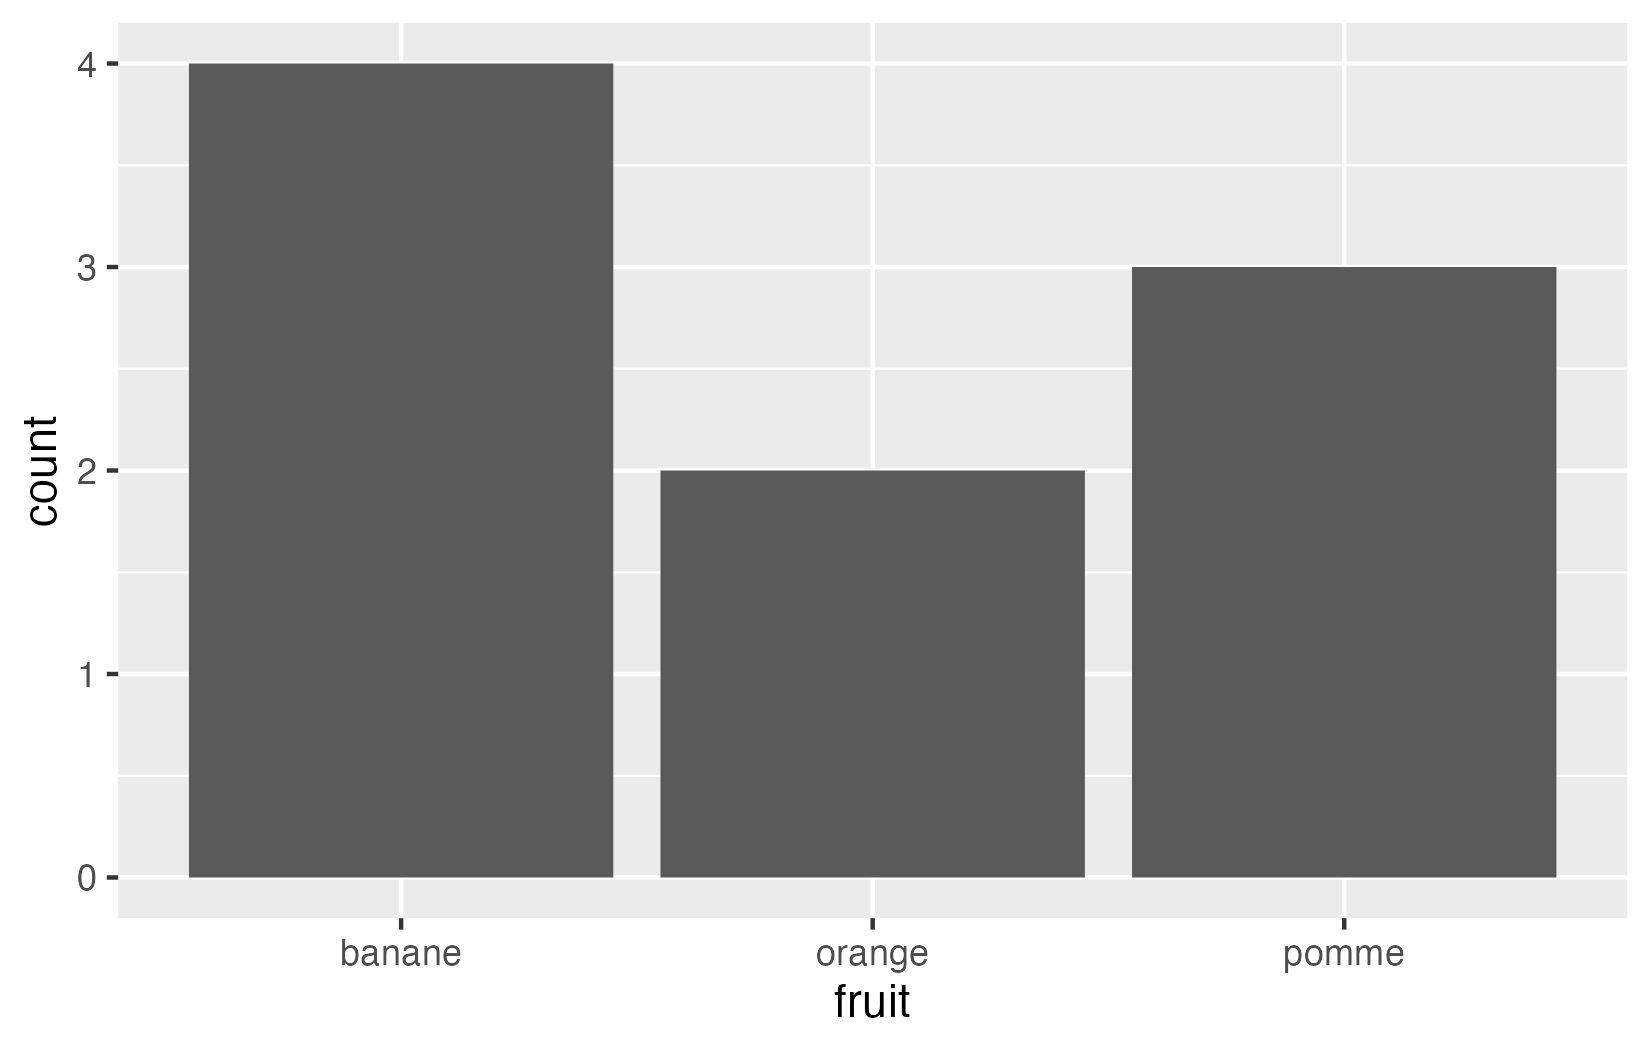
\includegraphics{./03-visualization_files/figure-pdf/fig-barplot-1.png}

}

\caption{\label{fig-barplot}Barplot pour des données non pré-comptées.}

\end{figure}

Pour visualiser les données déjà pré-comptées, on utilise
\texttt{geom\_col()} :

\begin{Shaded}
\begin{Highlighting}[]
\FunctionTok{ggplot}\NormalTok{(panier\_counted, }\FunctionTok{aes}\NormalTok{(}\AttributeTok{x =}\NormalTok{ fruit, }\AttributeTok{y =}\NormalTok{ nombre)) }\SpecialCharTok{+}
  \FunctionTok{geom\_col}\NormalTok{()}
\end{Highlighting}
\end{Shaded}

\begin{figure}[H]

{\centering 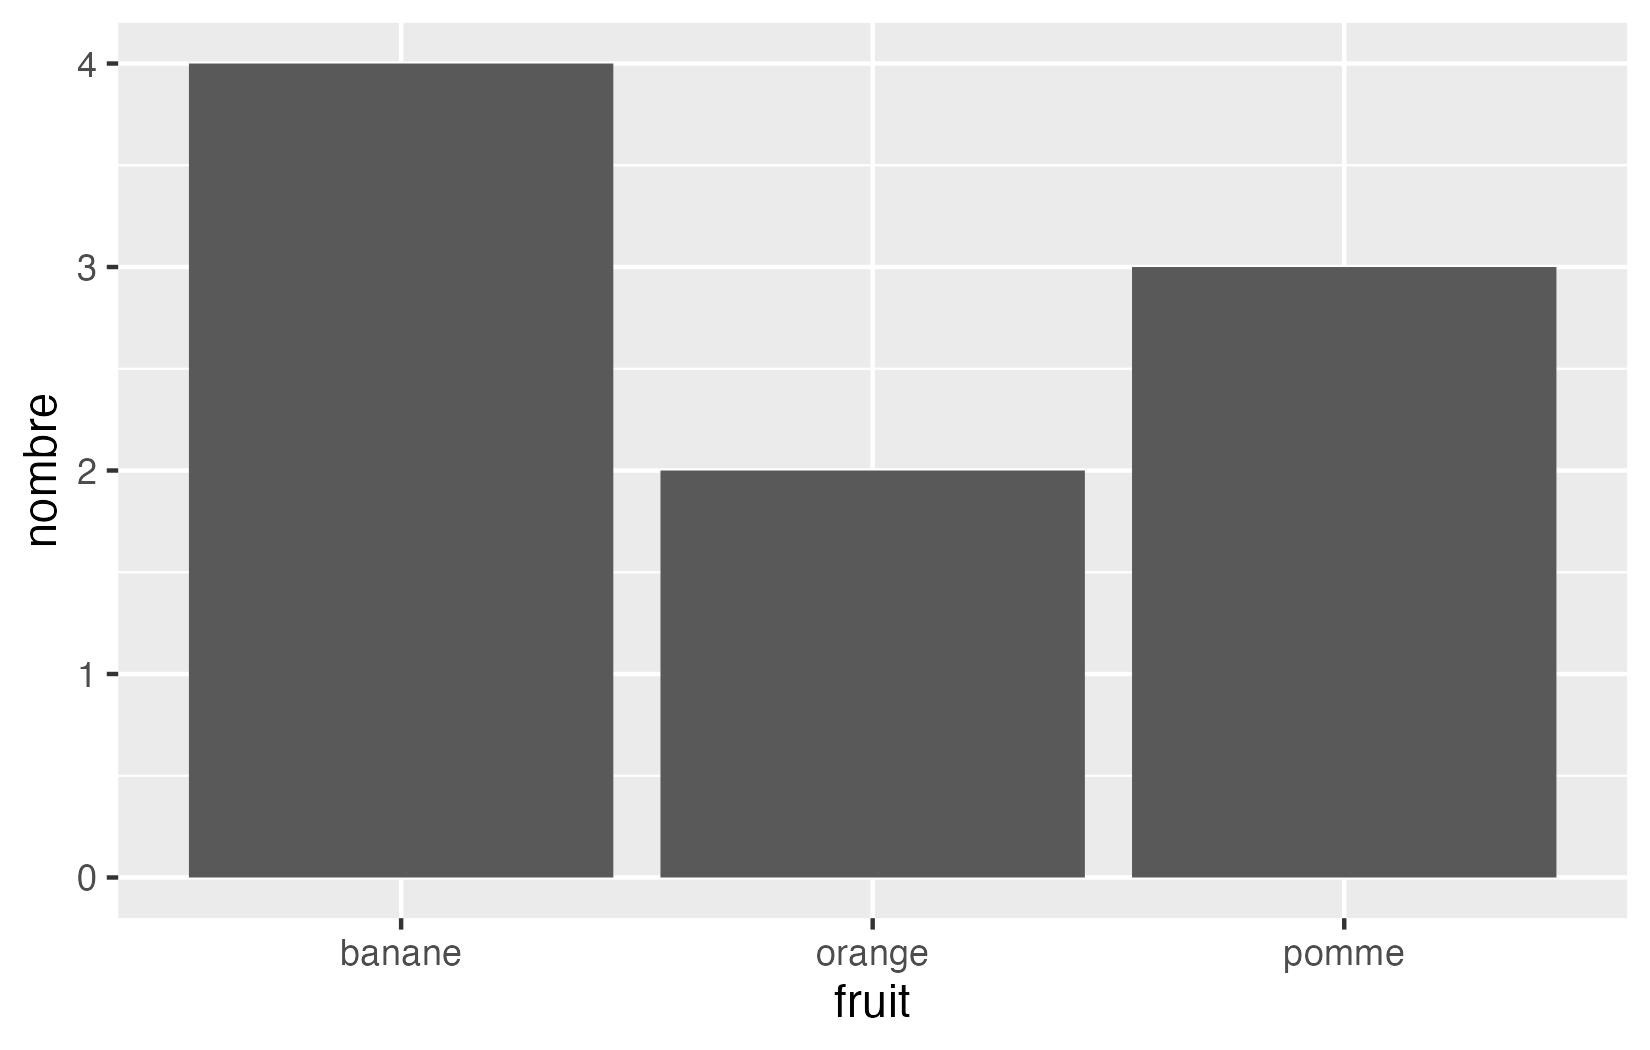
\includegraphics{./03-visualization_files/figure-pdf/fig-barplotcol-1.png}

}

\caption{\label{fig-barplotcol}Barplot pour des données pré-comptées.}

\end{figure}

Notez que les figures Figure~\ref{fig-barplot} et
Figure~\ref{fig-barplotcol} sont absolument identiques (à l'exception du
titre de l'axe des ordonnées), mais qu'elles ont été créées à partir de
2 tableaux de données différents. En particulier, notez que :

\begin{itemize}
\tightlist
\item
  Le code qui génère la figure Figure~\ref{fig-barplot} utilise le jeu
  de données \texttt{panier}, et n'associe pas de variable à l'axe des
  ordonnées : dans la fonction \texttt{aes()}, seule la variable
  associée à \texttt{x} est précisée. C'est la fonction
  \texttt{geom\_bar()} qui calcule automatiquement les abondances (ou
  fréquences) pour chaque catégorie de la variable \texttt{fruit}. La
  variable \texttt{count} est ainsi générée automatiquement et associée
  à \texttt{y}.
\item
  Le code qui génère la figure Figure~\ref{fig-barplotcol} utilise le
  jeu de données \texttt{panier\_counted}. Ici, c'est bien l'utilisateur
  qui associe la variable \texttt{nombre} à l'axe des \texttt{y} à
  l'intérieur de la fonction \texttt{aes()}. La fonction
  \texttt{geom\_col()} a besoin de 2 variables (une variable
  catégorielle pour l'axe des \texttt{x} et une numérique pour l'axe des
  \texttt{y}) pour fonctionner.
\end{itemize}

Autrement dit, lorsque vous souhaiterez créer un diagramme bâtons, il
faudra donc au préalable vérifier de quel type de données vous disposez
pour choisir l'objet géométrique approprié :

\begin{tcolorbox}[enhanced jigsaw, bottomtitle=1mm, title=\textcolor{quarto-callout-important-color}{\faExclamation}\hspace{0.5em}{Diagrammes bâtons}, breakable, opacitybacktitle=0.6, coltitle=black, opacityback=0, toprule=.15mm, toptitle=1mm, titlerule=0mm, colback=white, rightrule=.15mm, arc=.35mm, leftrule=.75mm, bottomrule=.15mm, left=2mm, colframe=quarto-callout-important-color-frame, colbacktitle=quarto-callout-important-color!10!white]

\begin{itemize}
\tightlist
\item
  Si la variable catégorielle n'est pas pré-comptée dans le tableau de
  données \faIcon{arrow-right} \texttt{geom\_bar()}. La variable
  catégorielle est associée à l'esthétique \texttt{x} du graphique. On
  ne renseigne pas \texttt{y}.
\item
  Si la variable catégorielle est pré-comptée dans le tableau de données
  \faIcon{arrow-right} \texttt{geom\_col()}. La variable catégorielle
  est associée à l'esthétique \texttt{x} du graphique. On associe
  explicitement les comptages à l'esthétique \texttt{y} du graphique.
\end{itemize}

\end{tcolorbox}

Enfin, notez que l'ordre des modalité (ou catégories) qui apparaissent
sur l'axe des abscisses est l'ordre alphabétique : la modalité
\texttt{banane} apparaît à gauche, puis la modalité \texttt{orange} et
enfin la modalité \texttt{pomme}. Bien souvent, cet ordre alphabétique
n'est pas pertinent. Nous verrons plus loin comment faire pour trier les
catégories par ordre croissant ou décroissant. C'est en effet une
possibilité intéressante qui est impossible pour les histogrammes (car
l'axe des \texttt{x} porte une variable numérique continue qu'il est
impossible de ``mélanger''), mais souvent vivement recommandée pour les
diagrammes bâtons.

\hypertarget{un-exemple-concret}{%
\subsubsection{Un exemple concret}\label{un-exemple-concret}}

Revenons aux manchots. Imaginons que nous souhaitions connaître le
nombre d'individus étudiés pour chaque espèce. Dans le jeu de données
\texttt{penguins}, la variable \texttt{species} indique à quelle espèce
appartiennent chacun des 344 individus étudiés. Une façon simple de
représenter ces données est donc la suivante :

\begin{Shaded}
\begin{Highlighting}[]
\FunctionTok{ggplot}\NormalTok{(penguins, }\FunctionTok{aes}\NormalTok{(}\AttributeTok{x =}\NormalTok{ species)) }\SpecialCharTok{+}
  \FunctionTok{geom\_bar}\NormalTok{()}
\end{Highlighting}
\end{Shaded}

\begin{figure}[H]

{\centering 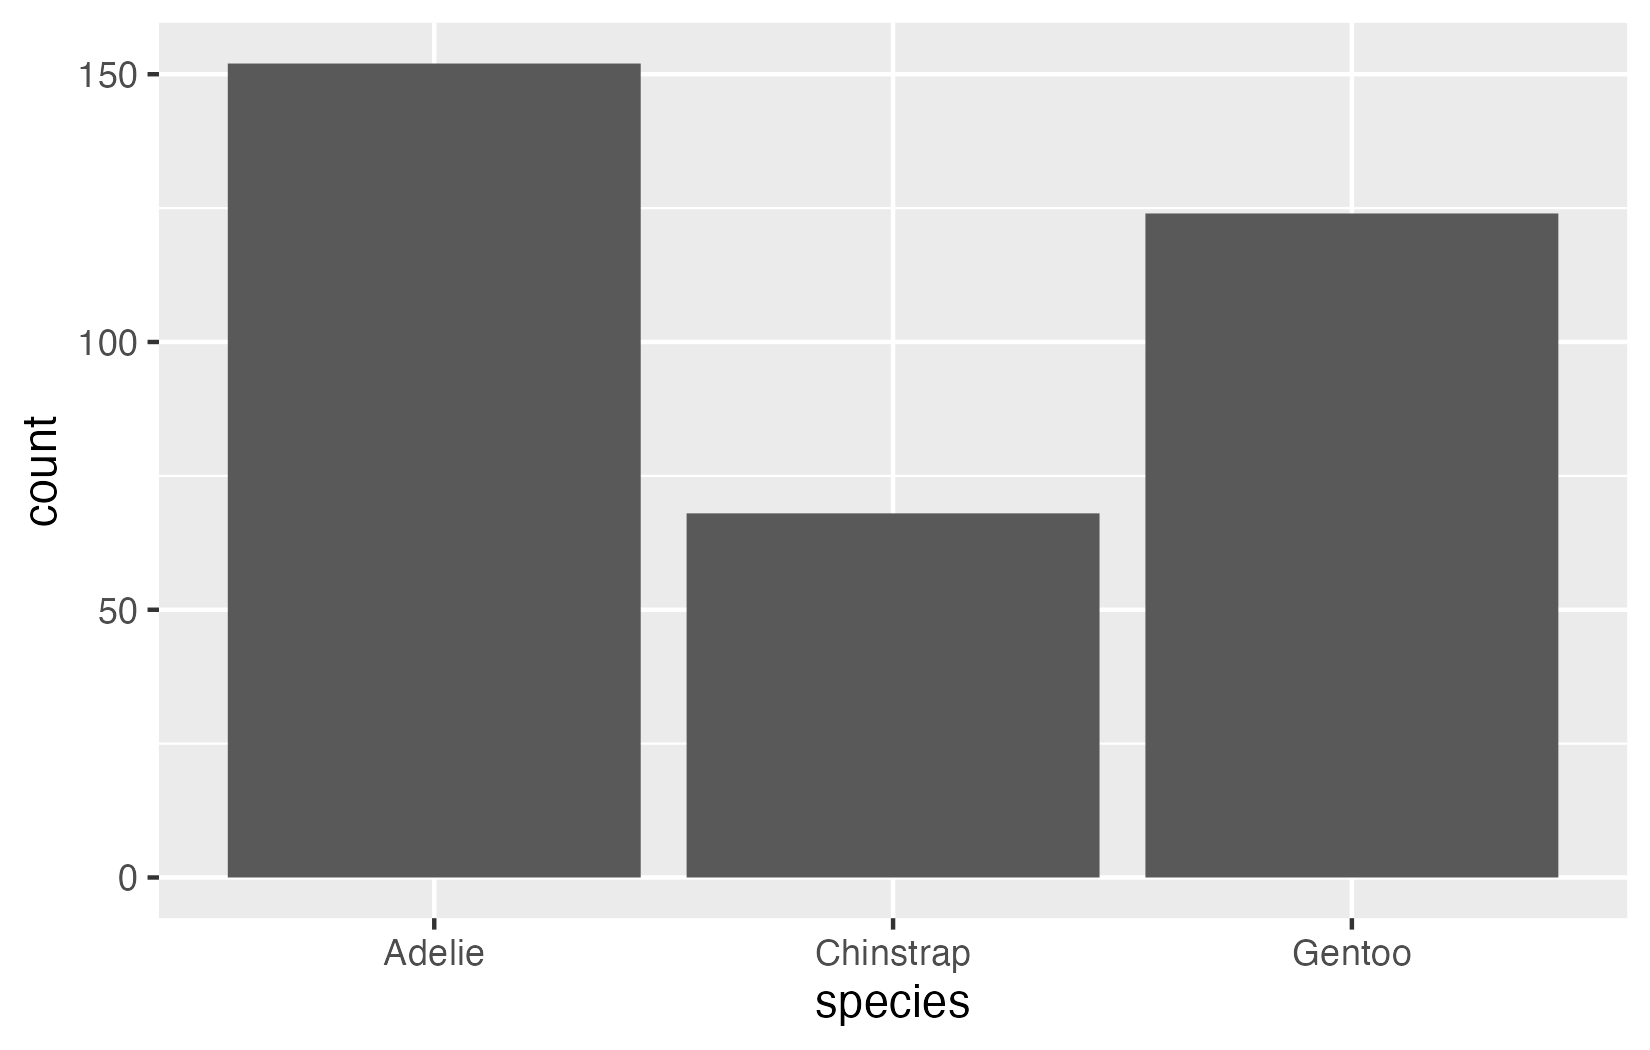
\includegraphics{./03-visualization_files/figure-pdf/fig-bpspecies-1.png}

}

\caption{\label{fig-bpspecies}Effectifs pour les 3 espèces de manchots
étudiées}

\end{figure}

Ici, \texttt{geom\_bar()} a compté le nombre d'occurrences de chaque
espèce dans le tableau \texttt{penguins} et a automatiquement associé ce
nombre à l'axe des ordonnées.

Là encore, les modalités sont triées par ordre alphabétique sur l'axe
des abscisses. Il est généralement plus utile de trier les catégories
par ordre décroissant. Nous pouvons faire cela facilement grâce à la
fonction \texttt{fct\_infreq()} du package \texttt{forcats}, qui permet
de modifier l'ordre des modalités d'une variable catégorielle (ou
facteur). Si vous avez installé le \texttt{tidyverse}, le package
\texttt{forcast} doit être disponible sur votre ordinateur. N'oubliez
pas de le charger si besoin :

\begin{Shaded}
\begin{Highlighting}[]
\FunctionTok{library}\NormalTok{(forcats)}
\FunctionTok{ggplot}\NormalTok{(penguins, }\FunctionTok{aes}\NormalTok{(}\AttributeTok{x =} \FunctionTok{fct\_infreq}\NormalTok{(species))) }\SpecialCharTok{+}
  \FunctionTok{geom\_bar}\NormalTok{()}
\end{Highlighting}
\end{Shaded}

\begin{figure}[H]

{\centering 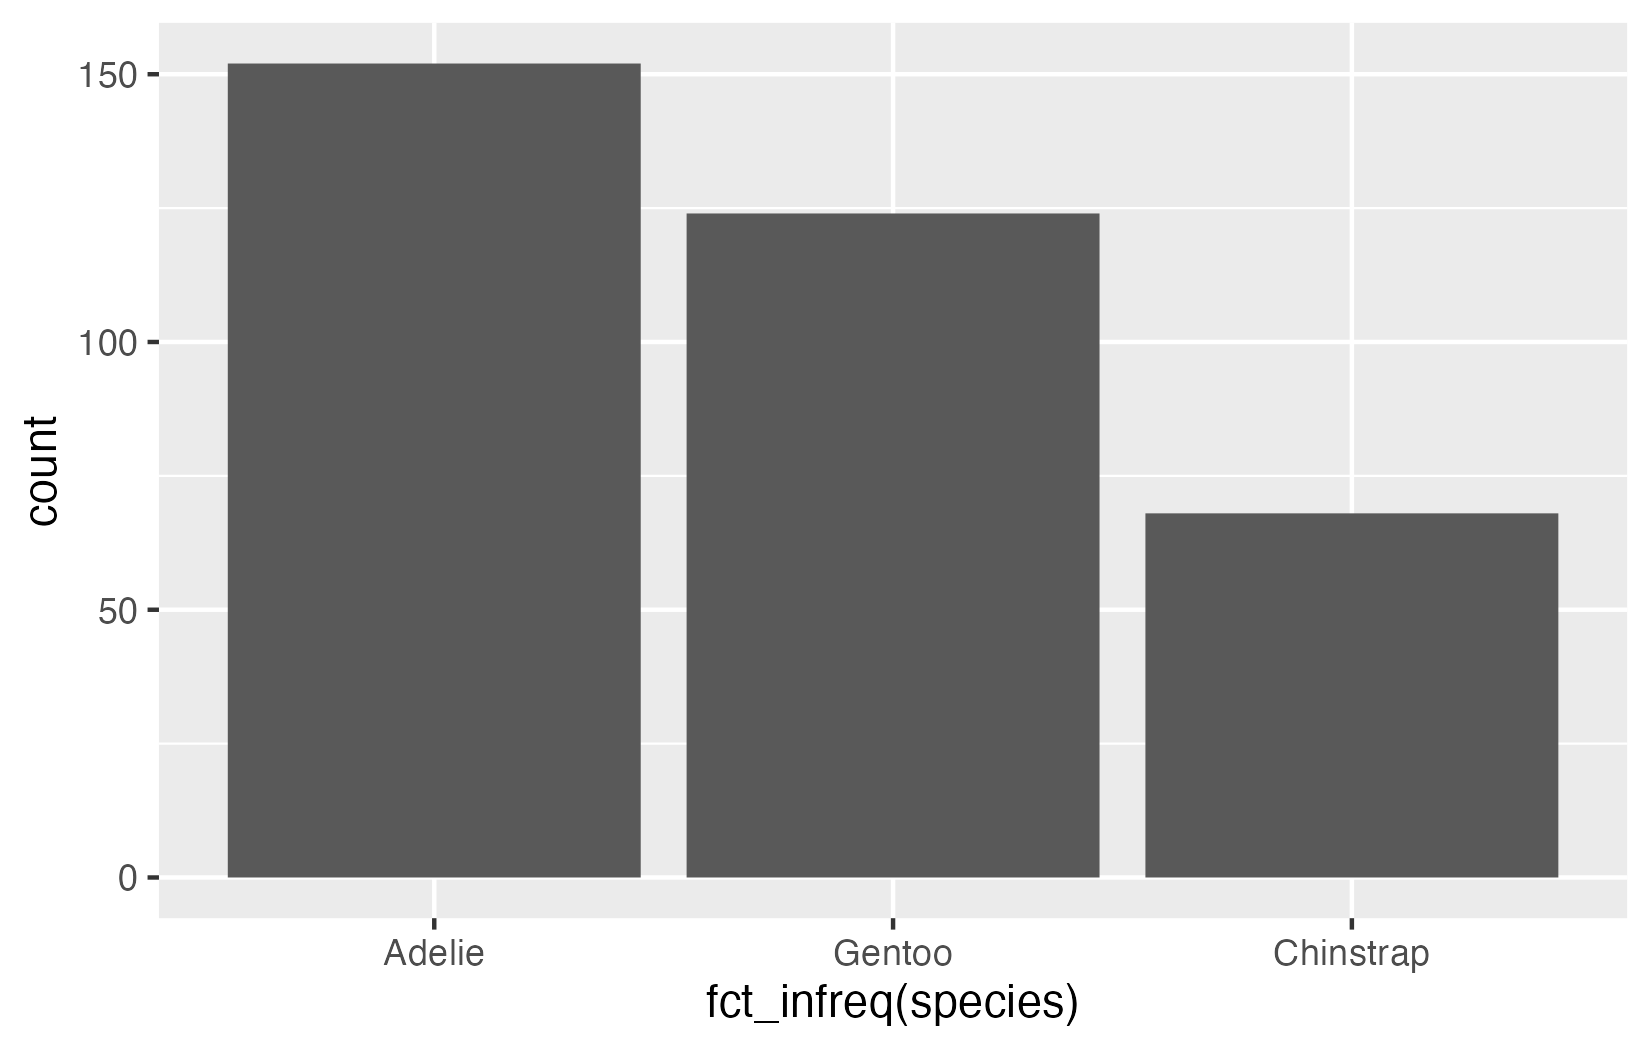
\includegraphics{./03-visualization_files/figure-pdf/fig-bpspecies-infreq-1.png}

}

\caption{\label{fig-bpspecies-infreq}Effectifs pour les 3 espèces de
manchots étudiées, triés en ordre décroissant}

\end{figure}

Ordonner les catégories par ordre décroissant est souvent indispensable
afin de faciliter la lecture du graphique et les comparaisons entre
catégories.

Si nous souhaitons connaître le nombre précis d'individus de chaque
espèce, il nous faut faire appel à plusieurs fonctions du package
\texttt{dplyr} que nous détaillerons dans le chapitre
Chapitre~\ref{sec-wrangling}. Ci-dessous, nous créons un nouveau tableau
\texttt{species\_table} contenant le nombre d'individus de chaque espèce
et les espèces sont ordonnées par abondance décroissante :

\begin{Shaded}
\begin{Highlighting}[]
\NormalTok{species\_table }\OtherTok{\textless{}{-}}\NormalTok{ penguins }\SpecialCharTok{\%\textgreater{}\%}   \CommentTok{\# On prend le tableau penguins, puis...}
  \FunctionTok{count}\NormalTok{(species) }\SpecialCharTok{\%\textgreater{}\%}            \CommentTok{\# On compte les effectifs de chaque espèce, puis...}
  \FunctionTok{arrange}\NormalTok{(}\FunctionTok{desc}\NormalTok{(n))              }\CommentTok{\# On trie par effectif décroissants ...}
\NormalTok{species\_table                   }\CommentTok{\# Enfin, on affiche la nouvelle table}
\end{Highlighting}
\end{Shaded}

\begin{verbatim}
# A tibble: 3 x 2
  species       n
  <fct>     <int>
1 Adelie      152
2 Gentoo      124
3 Chinstrap    68
\end{verbatim}

Ici, la table a été triée par effectifs décroissants. Mais attention,
\textbf{les niveaux} du facteur \texttt{species} n'ont pas été modifiés
:

\begin{Shaded}
\begin{Highlighting}[]
\FunctionTok{factor}\NormalTok{(species\_table}\SpecialCharTok{$}\NormalTok{species)}
\end{Highlighting}
\end{Shaded}

\begin{verbatim}
[1] Adelie    Gentoo    Chinstrap
Levels: Adelie Chinstrap Gentoo
\end{verbatim}

Le premier niveau est toujours \texttt{Adélie}, puis \texttt{Chinstrap},
en enfin \texttt{Gentoo}, et non pas l'ordre du tableau nouvellement
créé (\texttt{Adelie}, puis \texttt{Gentoo}, puis \texttt{Chinstrap})
car les niveaux sont toujours triés par ordre alphabétique. La
conséquence est que si nous devions faire un diagramme bâtons avec ces
données, la fonction \texttt{geom\_col()} ne permettrait pas d'ordonner
les catégories correctement :

\begin{Shaded}
\begin{Highlighting}[]
\FunctionTok{ggplot}\NormalTok{(species\_table, }\FunctionTok{aes}\NormalTok{(}\AttributeTok{x =}\NormalTok{ species, }\AttributeTok{y =}\NormalTok{ n)) }\SpecialCharTok{+}
  \FunctionTok{geom\_col}\NormalTok{()}
\end{Highlighting}
\end{Shaded}

\begin{figure}[H]

{\centering 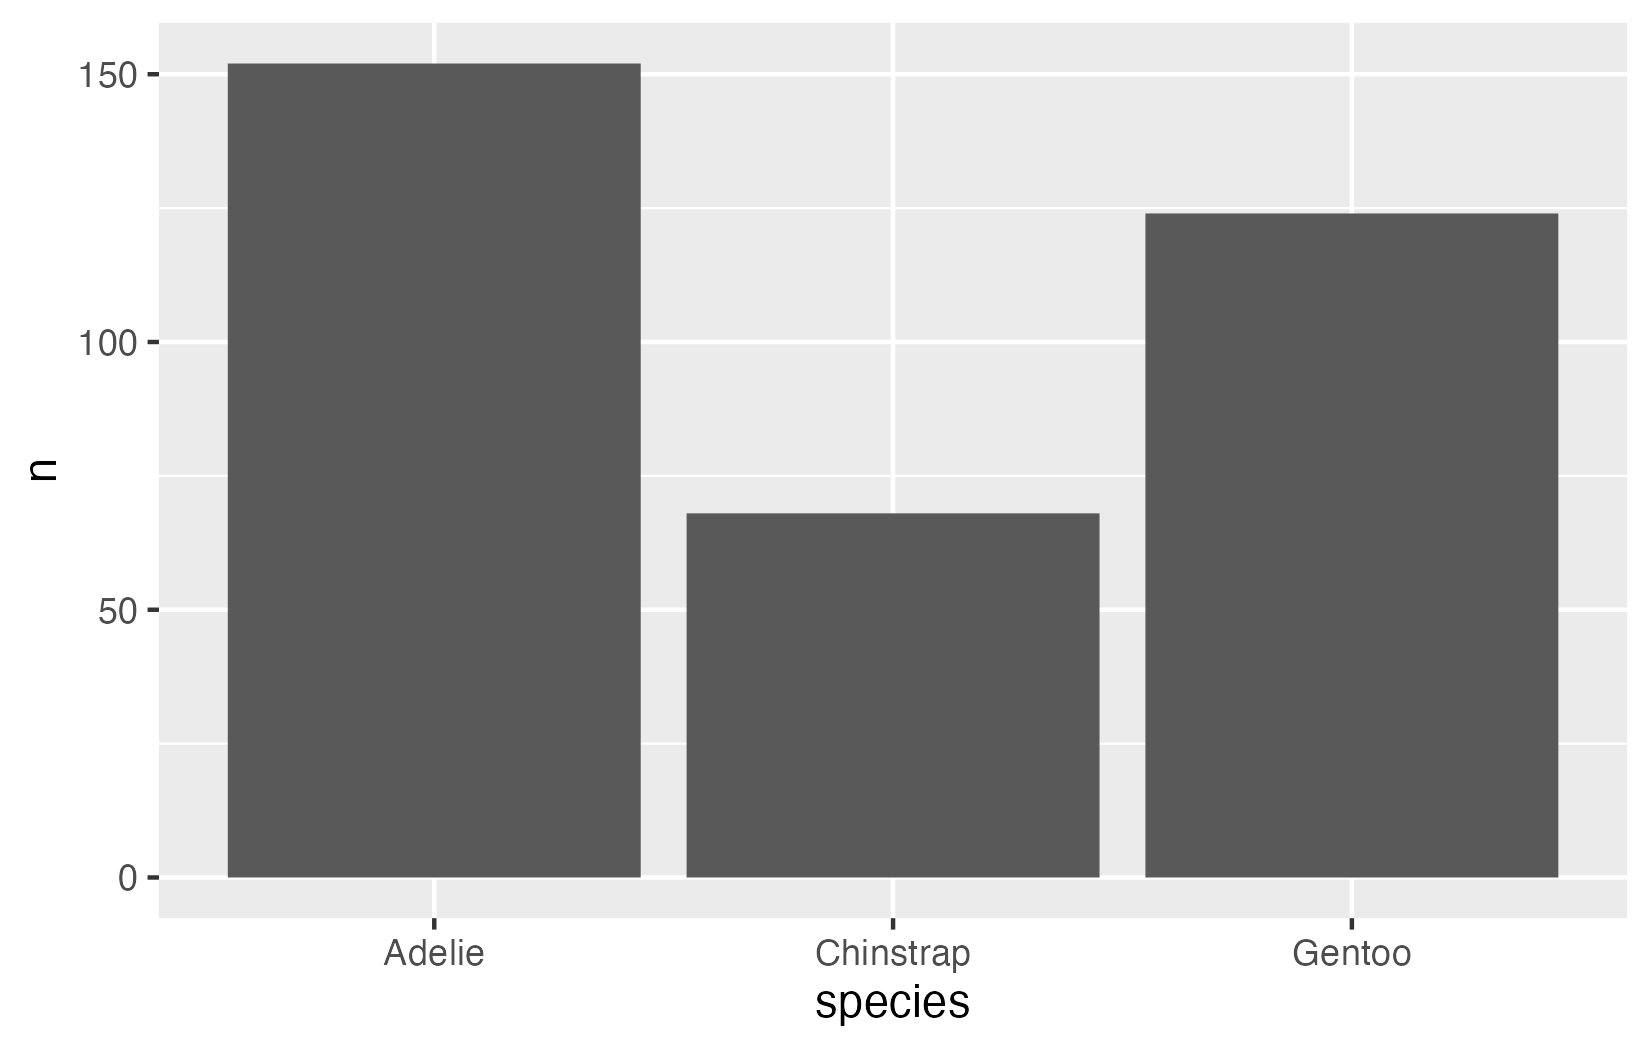
\includegraphics{./03-visualization_files/figure-pdf/unnamed-chunk-42-1.png}

}

\end{figure}

Si nous souhaitons trier ces catégories par effectif décroissant, la
fonction \texttt{fct\_infreq()} ne nous est ici d'aucune utilité. En
effet, le tableau \texttt{species\_table} contient une seule ligne pour
chaque espèce, donc une fréquence de \texttt{1} pour chaque espèce. Le
critère de la fréquence d'occurrence des modalités dans le tableau de
données ne peut donc pas être utilisé. Pour parvenir à nos fins avec ce
tableau déjà précompté, il faut cette fois utiliser la fonction
\texttt{fct\_reorder()} pour ordonner correctement les catégories. Cette
fonction prends 3 arguments :

\begin{enumerate}
\def\labelenumi{\arabic{enumi}.}
\tightlist
\item
  La variable catégorielle dont on souhaite réordonner les niveaux (ici,
  la variable \texttt{species} du tableau \texttt{species\_table}).
\item
  Une variable numérique qui permet d'ordonner les catégories (ici, la
  variable \texttt{n} du même tableau).
\item
  L'argument optionnel \texttt{.desc} qui permet de préciser si le tri
  doit être fait en ordre croissant (c'est le cas par défaut) ou
  décroissant.
\end{enumerate}

\begin{Shaded}
\begin{Highlighting}[]
\FunctionTok{ggplot}\NormalTok{(species\_table, }
       \FunctionTok{aes}\NormalTok{(}\AttributeTok{x =} \FunctionTok{fct\_reorder}\NormalTok{(species, n, }\AttributeTok{.desc =} \ConstantTok{TRUE}\NormalTok{), }\AttributeTok{y =}\NormalTok{ n)) }\SpecialCharTok{+}
  \FunctionTok{geom\_col}\NormalTok{()}
\end{Highlighting}
\end{Shaded}

\begin{figure}[H]

{\centering 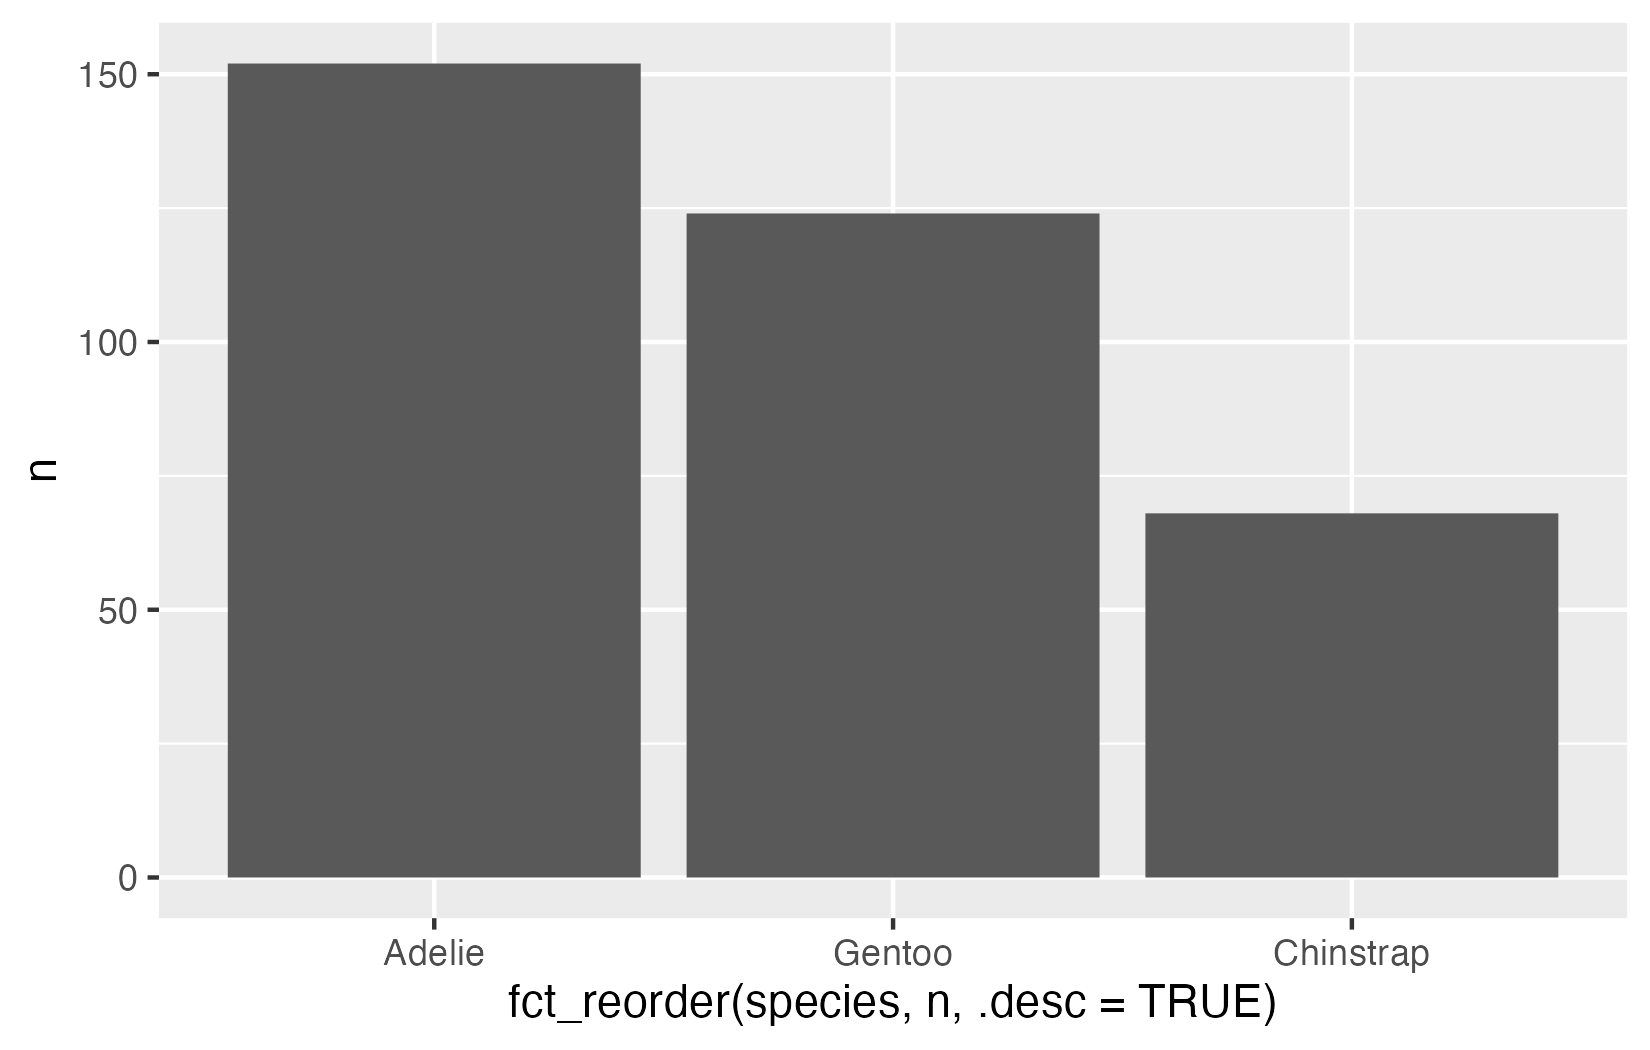
\includegraphics{./03-visualization_files/figure-pdf/unnamed-chunk-43-1.png}

}

\end{figure}

Vous voyez donc que selon le type de données dont vous disposez (soit un
tableau comme \texttt{penguins}, avec toutes les observations, soit un
tableau beaucoup plus compact comme \texttt{species\_table}), la
démarche permettant de produire un diagramme bâtons, dans lequel les
catégories seront triées, sera différente.

Une dernière précision : inverser l'ordre des variables sur les axes du
graphiques permet de faire un diagramme bâtons horizontal. C'est parfois
très utile lorsque les modalités de la variable catégorielle sont
nombreuses et/ou que leur nom est long. Faire apparaître les modalités
sur l'axe des \texttt{y} au lieu de l'axe des \texttt{x} peut rendre
leur lecture plus aisée :

\begin{Shaded}
\begin{Highlighting}[]
\FunctionTok{ggplot}\NormalTok{(penguins, }\FunctionTok{aes}\NormalTok{(}\AttributeTok{y =} \FunctionTok{fct\_infreq}\NormalTok{(species))) }\SpecialCharTok{+}
  \FunctionTok{geom\_bar}\NormalTok{(}\AttributeTok{fill =} \StringTok{"steelblue"}\NormalTok{, }\AttributeTok{color =} \StringTok{"black"}\NormalTok{, }\AttributeTok{alpha =} \FloatTok{0.7}\NormalTok{)}
\end{Highlighting}
\end{Shaded}

\begin{figure}[H]

{\centering 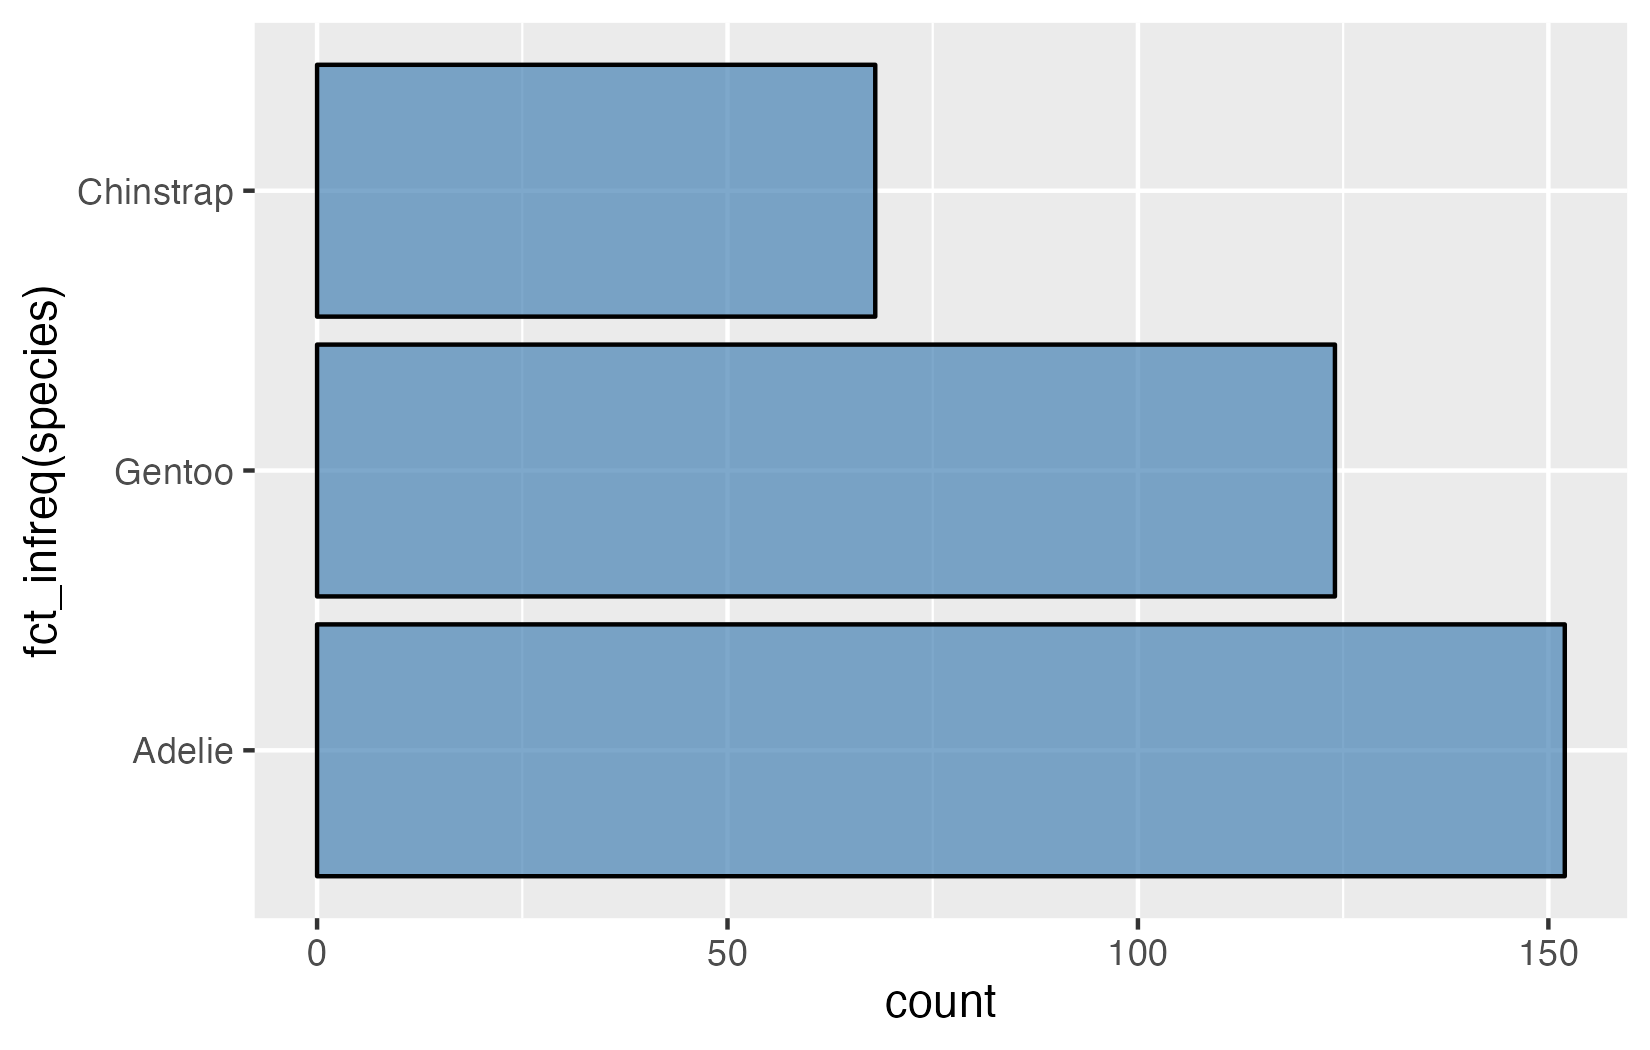
\includegraphics{./03-visualization_files/figure-pdf/unnamed-chunk-44-1.png}

}

\end{figure}

\begin{Shaded}
\begin{Highlighting}[]
\FunctionTok{ggplot}\NormalTok{(species\_table, }
       \FunctionTok{aes}\NormalTok{(}\AttributeTok{y =} \FunctionTok{fct\_reorder}\NormalTok{(species, n, }\AttributeTok{.desc =} \ConstantTok{TRUE}\NormalTok{), }\AttributeTok{x =}\NormalTok{ n)) }\SpecialCharTok{+}
  \FunctionTok{geom\_col}\NormalTok{(}\AttributeTok{fill =} \StringTok{"firebrick"}\NormalTok{, }\AttributeTok{color =} \StringTok{"black"}\NormalTok{, }\AttributeTok{alpha =} \FloatTok{0.7}\NormalTok{)}
\end{Highlighting}
\end{Shaded}

\begin{figure}[H]

{\centering 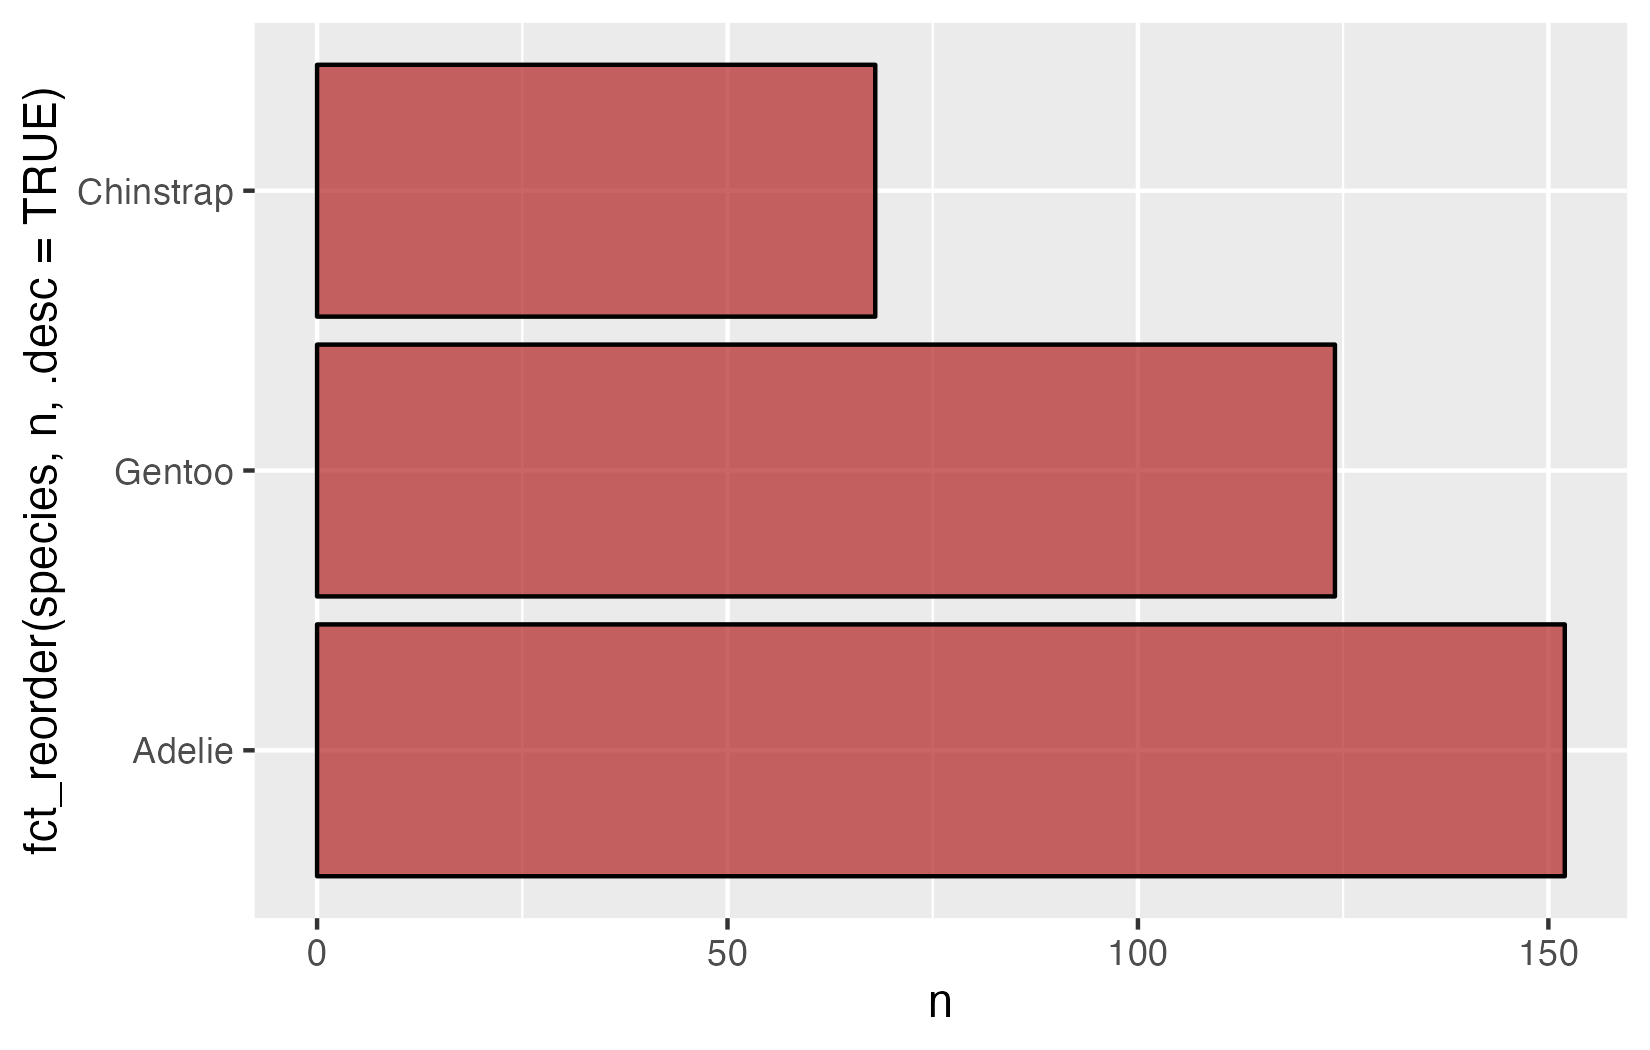
\includegraphics{./03-visualization_files/figure-pdf/unnamed-chunk-44-2.png}

}

\end{figure}

\hypertarget{sec-Exo-6}{%
\subsubsection{Exercices}\label{sec-Exo-6}}

\begin{enumerate}
\def\labelenumi{\arabic{enumi}.}
\tightlist
\item
  Quelle est la différence entre un histogramme et un diagramme bâtons ?
\item
  Pourquoi les histogrammes sont-ils inadaptés pour visualiser des
  données catégorielles ?
\item
  Pourquoi ne peut-on pas trier un histogramme par ordre croissant ?
\item
  Quelle île de l'archipel Palmer a fourni le plus grand nombre de
  manchots pour cette étude ?
\end{enumerate}

\hypertarget{uxe9viter-uxe0-tout-prix-les-diagrammes-circulaires}{%
\subsection{Éviter à tout prix les diagrammes
circulaires}\label{uxe9viter-uxe0-tout-prix-les-diagrammes-circulaires}}

À mon grand désarroi, l'un des graphiques classiquement utilisé pour
représenter la distribution d'une variable catégorielle est le diagramme
circulaire (ou diagramme camembert, piechart en anglais). C'est presque
toujours \textbf{la plus mauvaise visualisation possible} pour
représenter les effectifs ou pourcentages associés aux modalités d'une
variable catégorielle. Je vous demande de l'éviter à tout prix. Notre
cerveau n'est en effet pas correctement équipé pour comparer des angles
et des surfaces. Ainsi, par exemple, nous avons naturellement tendance à
surestimer les angles supérieurs à 90º, et à sous-estimer les angles
inférieurs à 90º. En d'autres termes, il est difficile pour les humains
de comparer des grandeurs sur des diagrammes circulaires.

À titre d'exemple, examinez ce diagramme, qui reprend les mêmes chiffres
que précédemment, et tentez de répondre aux questions suivantes :

\begin{figure}

{\centering 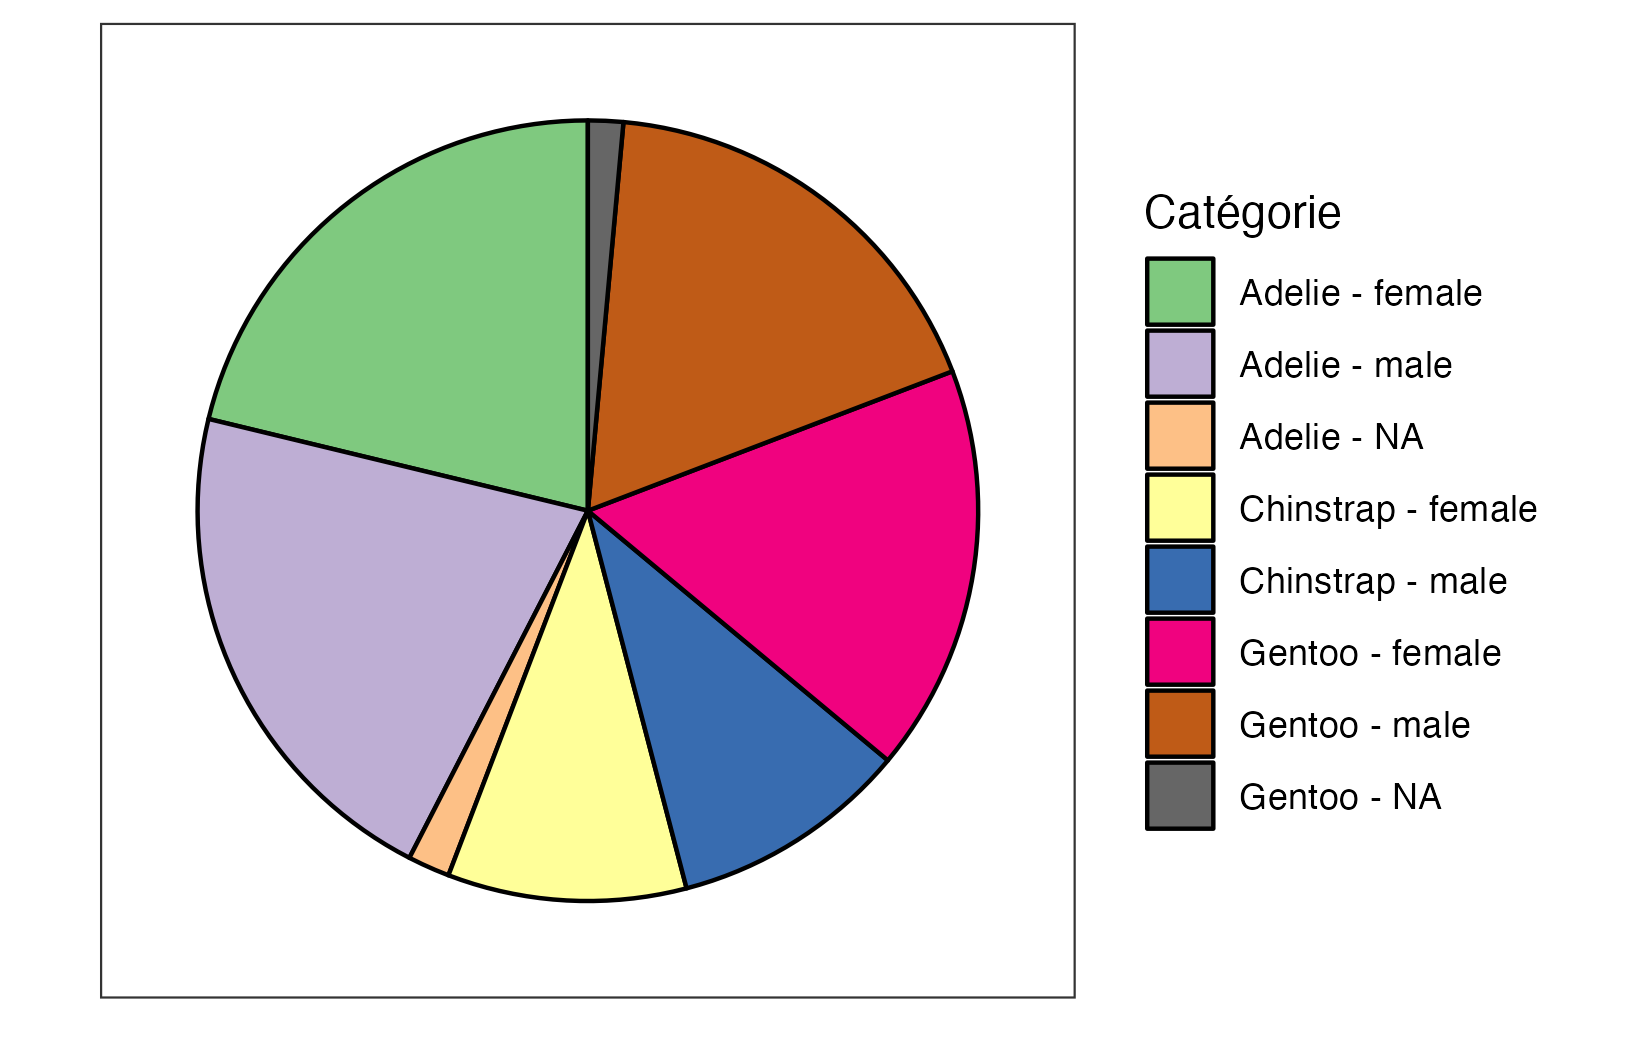
\includegraphics{./03-visualization_files/figure-pdf/fig-pie-1.png}

}

\caption{\label{fig-pie}Répartition des effectifs par espèce et par
sexe}

\end{figure}

\begin{itemize}
\tightlist
\item
  Quelle est la catégorie la plus représentée ?
\item
  De combien de fois la part des Gentoo mâles est-elle supérieure à
  celle des Chinstrap femelles ? (1,5 fois, 2 fois, 2.5 fois ?\ldots)
\item
  Quelle est la quatrième catégorie la plus représentée ?
\end{itemize}

Il est difficile (voir impossible) de répondre précisément à ces
questions avec le diagramme circulaire de la Figure~\ref{fig-pie}, alors
qu'il est très simple d'obtenir des réponses précises avec un diagramme
bâtons tel que présenté à la Figure~\ref{fig-bpspecies-sex} ci-dessous
(vérifiez-le !) :

\begin{figure}

{\centering 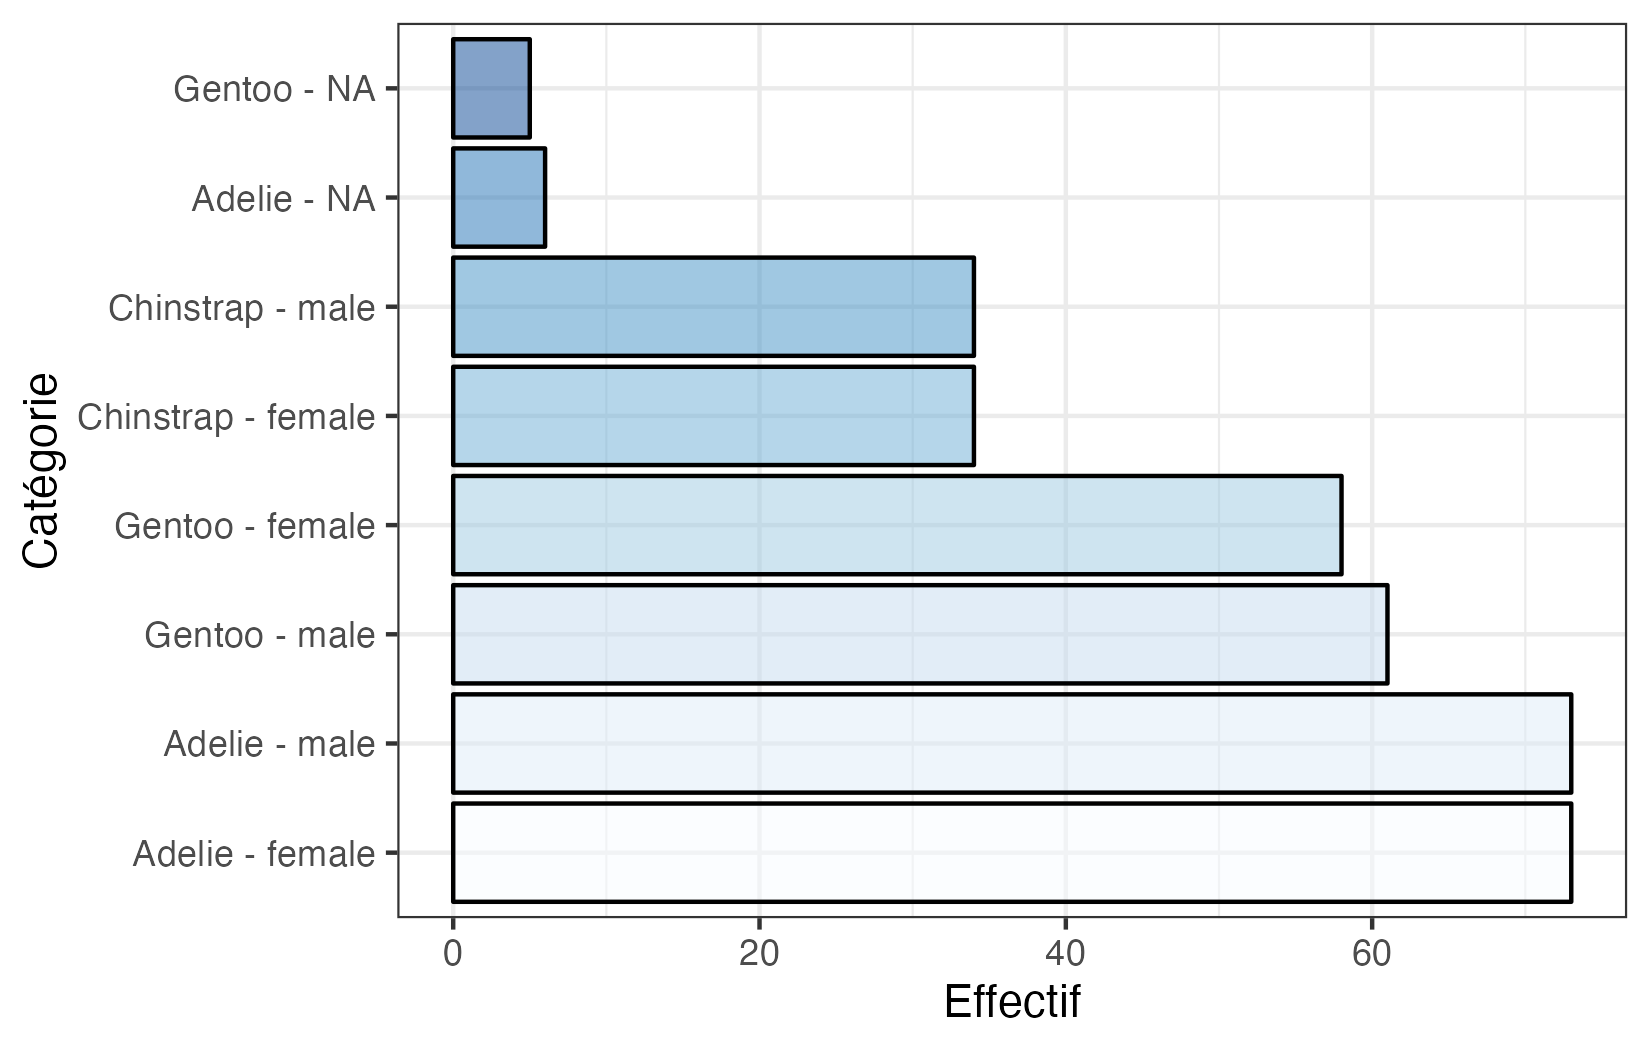
\includegraphics{./03-visualization_files/figure-pdf/fig-bpspecies-sex-1.png}

}

\caption{\label{fig-bpspecies-sex}Répartition des effectifs par espèce
et par sexe}

\end{figure}

\hypertarget{deux-variables-numuxe9riques}{%
\section{Deux variables numériques}\label{deux-variables-numuxe9riques}}

La représentation graphique la plus adaptée à la visualisation des
relations entre deux variables numériques est aussi l'une des plus
simples : il s'agit des nuages de points que nous avons déjà évoqués.
Ici dépendant, puisque nous disposons de 2 variables numériques, nous
allons en associer une à l'axe des \texttt{x} et l'autre à l'axe des
\texttt{y}. Si l'on pressent que l'une des deux variables pourrait
``expliquer'' la seconde, ou être en partie responsable de ses
variations, on l'appelle \textbf{variable explicative} et on la placera
alors sur l'axe des \texttt{x}. L'autre variable, celle que l'on suppose
influencée par la première est appelée \textbf{variable expliquée}, et
sera associée à l'axe des \texttt{y}.

Les nuages de points de 2 variables numériques permettent donc de
visualiser les relations (supposées ou réelles) entre deux variables.

\hypertarget{nuage-de-points}{%
\subsection{Nuage de points}\label{nuage-de-points}}

\hypertarget{syntaxe-uxe9luxe9mentaire-1}{%
\subsubsection{Syntaxe élémentaire}\label{syntaxe-uxe9luxe9mentaire-1}}

Prenons un exemple : nous souhaitons examiner les relations qui existent
entre la masse corporelle des individus et la longueur de leur nageoire.
Une relation allométrique simple suppose en effet que plus un individu
est grand et lourd, plus ses membres seront développés. La nature de la
relation allométrique peut toutefois être radicalement différente selon
les espèces. Pour l'instant, nous ne nous intéressons pas aux
éventuelles différences entre espèces et nous examinerons donc
l'ensemble des données, toutes espèces confondues.

\begin{Shaded}
\begin{Highlighting}[]
\FunctionTok{ggplot}\NormalTok{(penguins, }\FunctionTok{aes}\NormalTok{(}\AttributeTok{x =}\NormalTok{ body\_mass\_g, }\AttributeTok{y =}\NormalTok{ flipper\_length\_mm)) }\SpecialCharTok{+}
  \FunctionTok{geom\_point}\NormalTok{()}
\end{Highlighting}
\end{Shaded}

\begin{verbatim}
Warning: Removed 2 rows containing missing values (geom_point).
\end{verbatim}

\begin{figure}[H]

{\centering 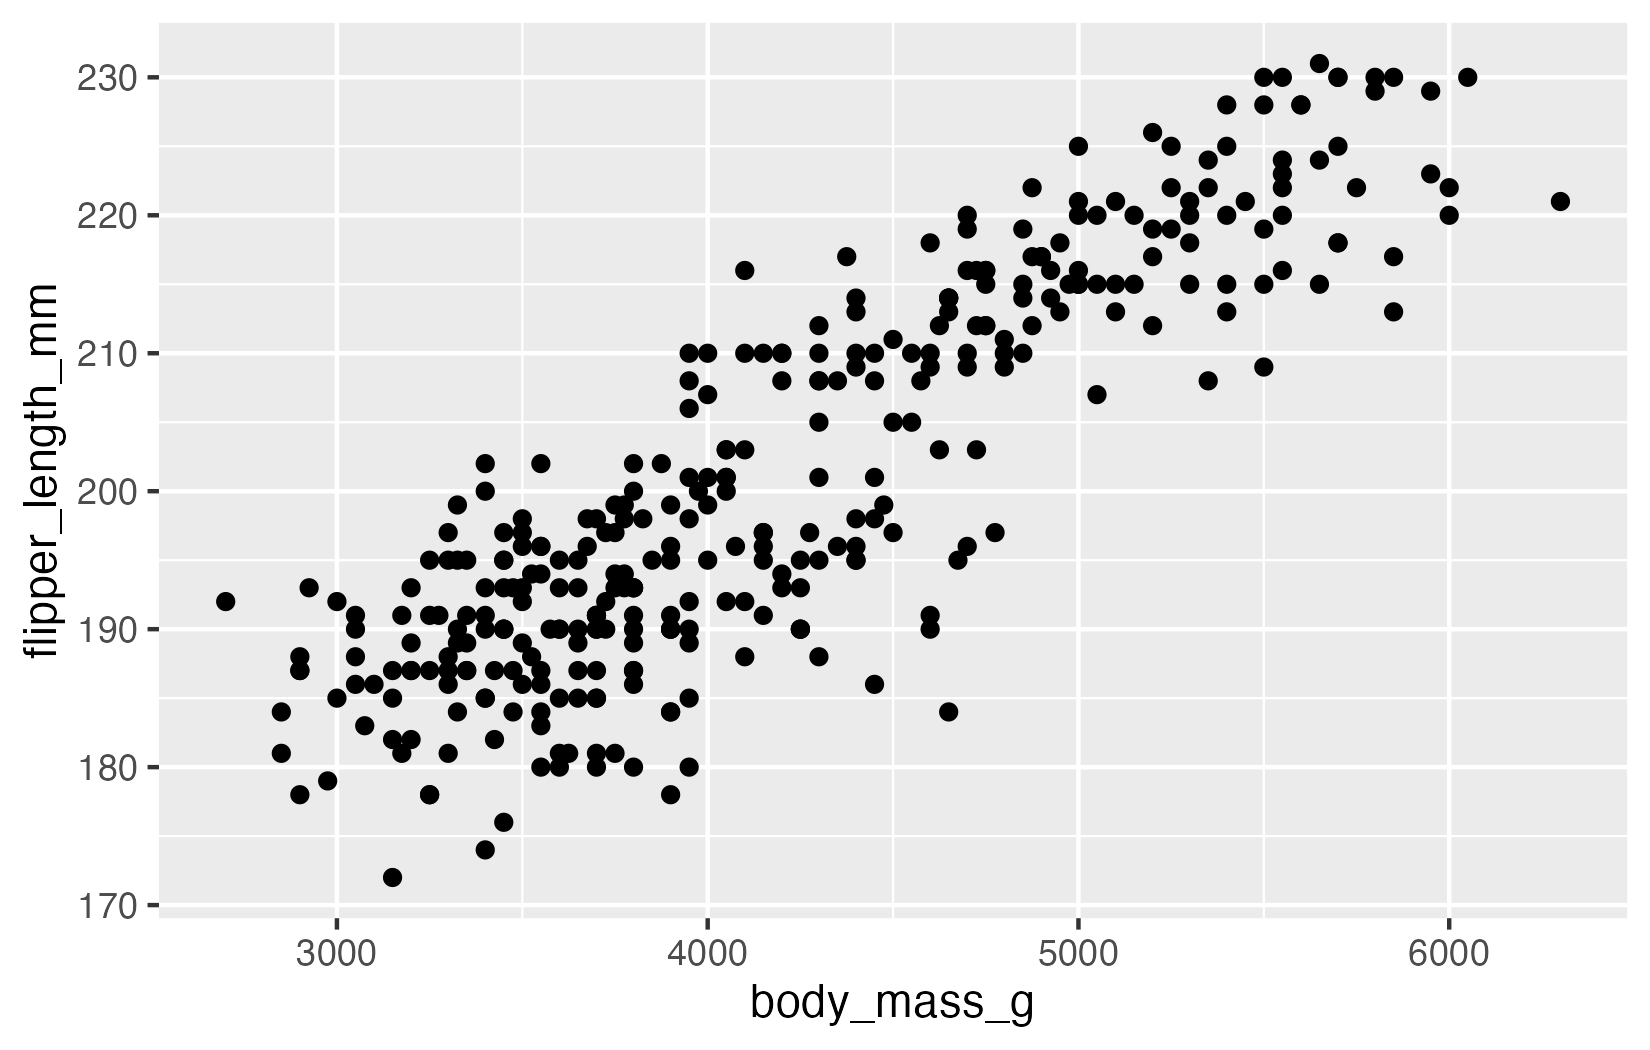
\includegraphics{./03-visualization_files/figure-pdf/unnamed-chunk-47-1.png}

}

\end{figure}

Ici, j'associe \texttt{body\_mass\_g} à l'axe des \texttt{x} car je
suppose que c'est la variable explicative. Il est en effet plus logique
de considérer que la masse corporelle influence la longueur des
nageoires plutôt que le contraire. La variable expliquée, ici
\texttt{flipper\_length\_mm} est associée à l'axe des \texttt{y}.

La syntaxe est donc très simple, et le graphique obtenu permet de
constater que plus les individus sont lourds, plus leurs nageoires sont
longues.

\hypertarget{droite-de-tendance}{%
\subsubsection{Droite de tendance}\label{droite-de-tendance}}

Si l'on souhaite visualiser (modéliser !) cette association entre les
deux variables, on peut ajouter sur ce graphique une courbe de tendance
ou une droite de régression avec l'objet géométrique
\texttt{geom\_smooth()} :

\begin{Shaded}
\begin{Highlighting}[]
\FunctionTok{ggplot}\NormalTok{(penguins, }\FunctionTok{aes}\NormalTok{(}\AttributeTok{x =}\NormalTok{ body\_mass\_g, }\AttributeTok{y =}\NormalTok{ flipper\_length\_mm)) }\SpecialCharTok{+}
  \FunctionTok{geom\_point}\NormalTok{() }\SpecialCharTok{+}
  \FunctionTok{geom\_smooth}\NormalTok{(}\AttributeTok{method =} \StringTok{"lm"}\NormalTok{)}
\end{Highlighting}
\end{Shaded}

\begin{verbatim}
`geom_smooth()` using formula 'y ~ x'
\end{verbatim}

\begin{verbatim}
Warning: Removed 2 rows containing non-finite values (stat_smooth).
\end{verbatim}

\begin{verbatim}
Warning: Removed 2 rows containing missing values (geom_point).
\end{verbatim}

\begin{figure}[H]

{\centering 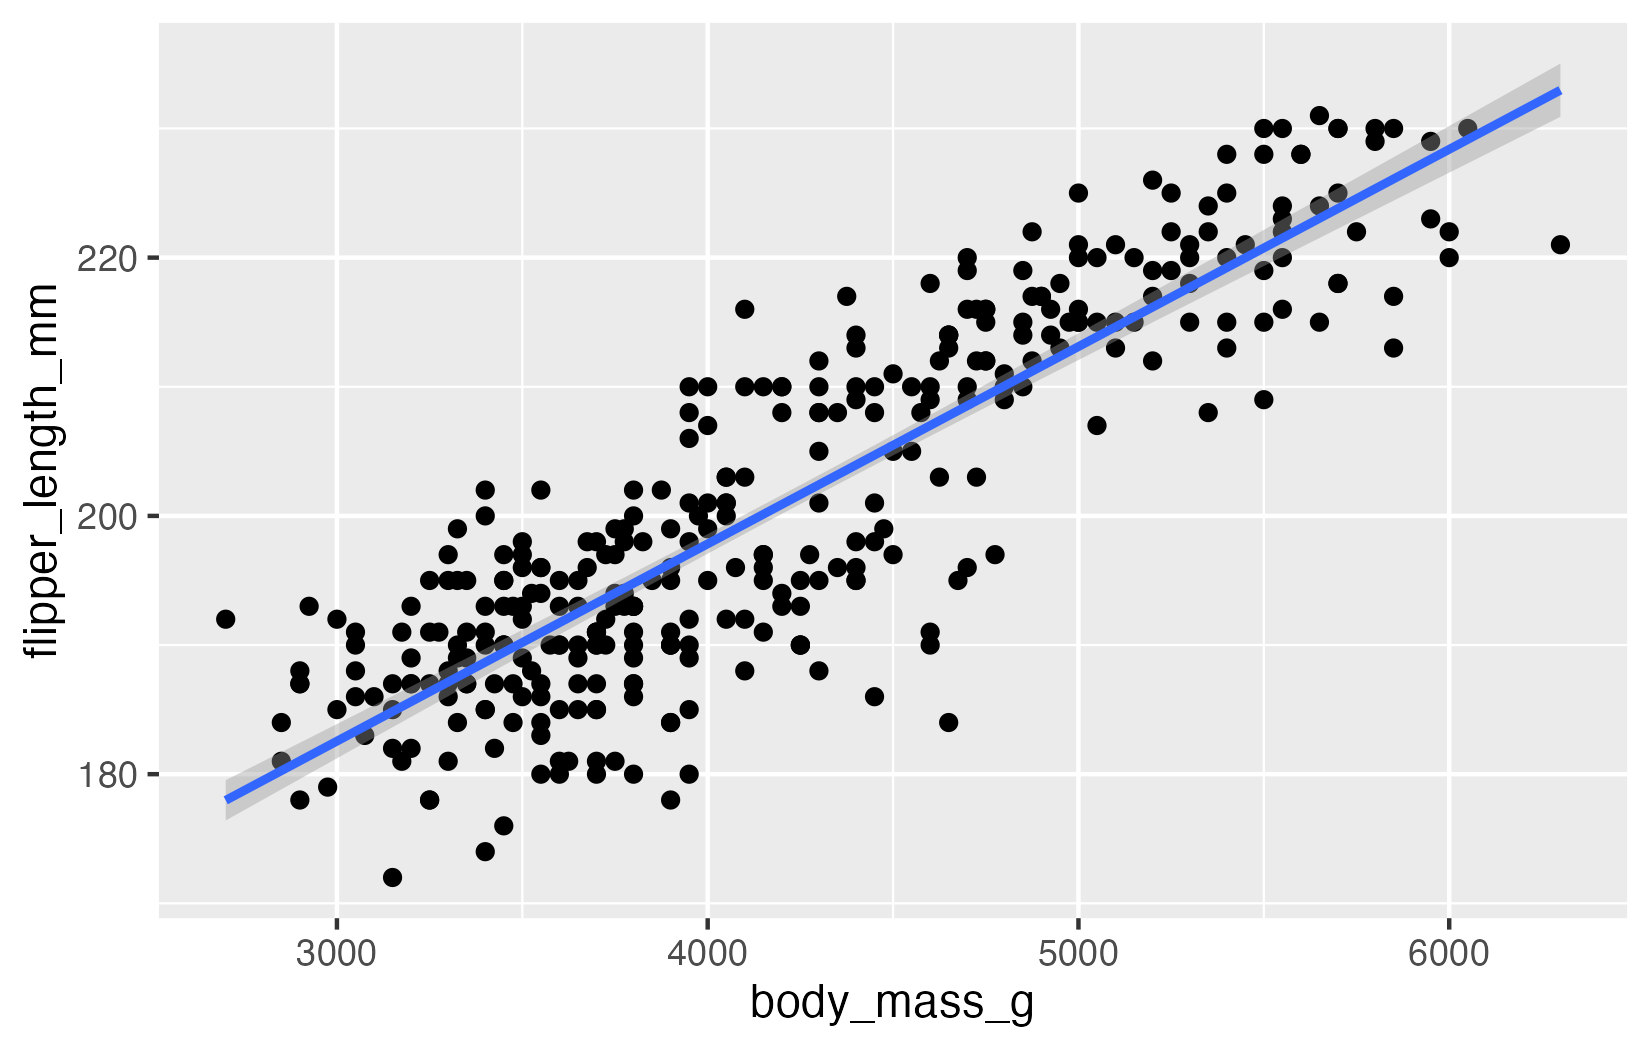
\includegraphics{./03-visualization_files/figure-pdf/unnamed-chunk-48-1.png}

}

\end{figure}

L'argument \texttt{method\ =\ "lm"} indique que nous souhaitons ajouter
une droite de régression (\texttt{lm} est l'abréviation de ``linear
model''). L'intervalle grisé autour de la droite représente
l'incertitude associée à la régression et indique que la ``vraie''
droite de régression, dans la population générale (et pas seulement dans
notre échantillon de 344 individus) est probablement située dans cette
zone grisée. Nous aurons l'occasion de revenir en détail sur la notion
de régression linéaire et d'incertitude associée au semestre 6 de la
licence SV.

\hypertarget{autres-caractuxe9ristiques-esthuxe9tiques}{%
\subsubsection{Autres caractéristiques
esthétiques}\label{autres-caractuxe9ristiques-esthuxe9tiques}}

Comme pour tous les graphiques faisant apparaître des points, il est
possible de modifier les caractéristiques esthétiques habituelles, soit
en les associant à des variables du jeu de données (et en l'indiquant à
l'intérieur de \texttt{aes()}), soit en les fixant à des valeurs
constantes qui s'appliqueront à tous les points (et en l'indiquant alors
en dehors de \texttt{aes()}). L'exemple ci-dessous illustre ces
possibilités :

\begin{Shaded}
\begin{Highlighting}[]
\FunctionTok{ggplot}\NormalTok{(penguins, }\FunctionTok{aes}\NormalTok{(}\AttributeTok{x =}\NormalTok{ body\_mass\_g, }\AttributeTok{y =}\NormalTok{ flipper\_length\_mm, }\AttributeTok{fill =}\NormalTok{ species)) }\SpecialCharTok{+}
  \FunctionTok{geom\_point}\NormalTok{(}\AttributeTok{shape =} \DecValTok{21}\NormalTok{, }\AttributeTok{color =} \StringTok{"black"}\NormalTok{, }\AttributeTok{alpha =} \FloatTok{0.6}\NormalTok{) }\SpecialCharTok{+}
  \FunctionTok{geom\_smooth}\NormalTok{(}\FunctionTok{aes}\NormalTok{(}\AttributeTok{color =}\NormalTok{ species), }\AttributeTok{method =} \StringTok{"lm"}\NormalTok{, }\AttributeTok{se =} \ConstantTok{FALSE}\NormalTok{)}
\end{Highlighting}
\end{Shaded}

\begin{verbatim}
`geom_smooth()` using formula 'y ~ x'
\end{verbatim}

\begin{verbatim}
Warning: Removed 2 rows containing non-finite values (stat_smooth).
\end{verbatim}

\begin{verbatim}
Warning: Removed 2 rows containing missing values (geom_point).
\end{verbatim}

\begin{figure}[H]

{\centering \includegraphics{./03-visualization_files/figure-pdf/unnamed-chunk-49-1.png}

}

\end{figure}

L'argument \texttt{se\ =\ FALSE} de la fonction \texttt{geom\_smooth()}
permet de ne pas afficher l'intervalle d'incertitude de la régression
linéaire. Ici, j'ai associé la couleur de remplissage des points et la
couleur des droites de régression aux espèces (donc à l'intérieur de
\texttt{aes()}, soit dans \texttt{ggplot()} soit dans
\texttt{geom\_smooth()}), et j'ai fixé pour tous les points, le choix du
type de symbole (\texttt{shape\ =\ 21}, voir Figure~\ref{fig-pch}), la
couleur de contour (\texttt{color\ =\ "black"}) et la transparence
\texttt{alpha\ =\ 0.6}.

Là encore, il ne s'agit plus strictement d'un graphique représentant les
relations entre 2 variables numériques, mais bien entre 3 variables :
deux variables numériques (\texttt{body\_mass\_g} et
\texttt{flipper\_length\_mm}) et une variable catégorielle ou facteur
(\texttt{species}). Il est finalement très simple d'ajouter d'autres
variables sur un graphique bivarié tel qu'un nuage de points.

\hypertarget{les-graphiques-en-lignes}{%
\subsection{Les graphiques en lignes}\label{les-graphiques-en-lignes}}

Les graphiques en lignes, ou ``linegraphs'' sont généralement utilisés
lorsque l'axe des \texttt{x} porte une information \textbf{temporelle},
et l'axe des \texttt{y} une autre variable numérique. Le temps est une
variable naturellement ordonnée : les jours, semaines, mois, années, se
suivent naturellement. Les graphiques en lignes devraient être évités
lorsqu'il n'y a pas une organisation séquentielle évidente de la
variable portée par l'axe des \texttt{x}. Ainsi, lorsque l'une des 2
variables dont on dispose est une variable numérique temporelle (des
dates, des heures, etc.), on la place sur l'axe des \texttt{x} et la
seconde variable, dont on étudiera les fluctuations au cours du temps,
sur l'axe des \texttt{y}. On peut alors relier les valeurs grâce à
l'objet géométrique \texttt{geom\_line()} afin de créer une série
temporelle. Pour illustrer cela, examinons un autre jeu de données qui
contient une variable temporelle :

\begin{Shaded}
\begin{Highlighting}[]
\NormalTok{economics}
\end{Highlighting}
\end{Shaded}

\begin{verbatim}
# A tibble: 574 x 6
   date         pce    pop psavert uempmed unemploy
   <date>     <dbl>  <dbl>   <dbl>   <dbl>    <dbl>
 1 1967-07-01  507. 198712    12.6     4.5     2944
 2 1967-08-01  510. 198911    12.6     4.7     2945
 3 1967-09-01  516. 199113    11.9     4.6     2958
 4 1967-10-01  512. 199311    12.9     4.9     3143
 5 1967-11-01  517. 199498    12.8     4.7     3066
 6 1967-12-01  525. 199657    11.8     4.8     3018
 7 1968-01-01  531. 199808    11.7     5.1     2878
 8 1968-02-01  534. 199920    12.3     4.5     3001
 9 1968-03-01  544. 200056    11.7     4.1     2877
10 1968-04-01  544  200208    12.3     4.6     2709
# ... with 564 more rows
\end{verbatim}

Le jeu de données \texttt{economics} est fourni avec le package
\texttt{ggplot2}. Puisque vous avez chargé ce package (ou le
\texttt{tidyverse} qui contient ce package), vous devriez pouvoir
accéder à ce tableau sans difficulté. Nous nous intéresserons ici à la
variable \texttt{date} que nous placerons sur l'axe des \texttt{x} et à
la variable \texttt{uempmed} qui est la durée de chômage médiane dans la
population américaine, en nombre de semaines, que nous placerons sur
l'axe des \texttt{y}. Examinons donc comment la durée médiane du du
chômage a évolué au fil du temps :

\begin{Shaded}
\begin{Highlighting}[]
\FunctionTok{ggplot}\NormalTok{(economics, }\FunctionTok{aes}\NormalTok{(}\AttributeTok{x =}\NormalTok{ date, }\AttributeTok{y =}\NormalTok{ uempmed)) }\SpecialCharTok{+}
  \FunctionTok{geom\_line}\NormalTok{()}
\end{Highlighting}
\end{Shaded}

\begin{figure}[H]

{\centering \includegraphics{./03-visualization_files/figure-pdf/unnamed-chunk-51-1.png}

}

\end{figure}

Notez que puisque la variable \texttt{date} du tableau
\texttt{economics} est comprise par \texttt{R} comme étant du type
``variable temporelle'' (le type indiqué dans le tableau, juste sous le
nom de variable, est \texttt{\textless{}date\textgreater{}}), l'axe des
abscisses du graphique, qui est associé à cette variable, est
correctement mis en forme : seules les années apparaissent.

Les graphiques en lignes permettent de visualiser des
progressions/évolutions lorsqu'il existe une temporalité entre les
données. Sur l'exemple, traité plus haut, du lien entre masse et
longueur des nageoire des manchots, relier les points n'aurait
absolument aucun sens puisque toutes les observations sont indépendantes
: elles correspondent à des individus différents. Soyez donc prudents
lorsque vous reliez les points dur un graphique. Cela n'est possible que
lorsque les données le permettent. Vous devez donc toujours vous poser
la question de la pertinence de vos choix de représentations.

Comme pour les autres types de graphiques, il est possible de modifier
les caractéristiques esthétiques des lignes sur un graphique, en
particulier :

\begin{itemize}
\tightlist
\item
  \texttt{color} : la couleur des lignes
\item
  \texttt{size} : l'épaisseur des lignes
\item
  \texttt{linetype} : le type de ligne (continue, pointillée, tirets,
  etc. Essayez plusieurs valeurs entières pour comparer les types de
  lignes)
\end{itemize}

\begin{Shaded}
\begin{Highlighting}[]
\FunctionTok{ggplot}\NormalTok{(economics, }\FunctionTok{aes}\NormalTok{(}\AttributeTok{x =}\NormalTok{ date, }\AttributeTok{y =}\NormalTok{ uempmed)) }\SpecialCharTok{+}
  \FunctionTok{geom\_line}\NormalTok{(}\AttributeTok{color =} \StringTok{"orange"}\NormalTok{, }\AttributeTok{linetype =} \DecValTok{2}\NormalTok{)}
\end{Highlighting}
\end{Shaded}

\begin{figure}[H]

{\centering \includegraphics{./03-visualization_files/figure-pdf/unnamed-chunk-52-1.png}

}

\end{figure}

L'argument \texttt{linetype} est également utilisable par l'objet
géométrique \texttt{geom\_smooth()} :

\begin{Shaded}
\begin{Highlighting}[]
\FunctionTok{ggplot}\NormalTok{(economics, }\FunctionTok{aes}\NormalTok{(}\AttributeTok{x =}\NormalTok{ date, }\AttributeTok{y =}\NormalTok{ uempmed)) }\SpecialCharTok{+}
  \FunctionTok{geom\_line}\NormalTok{() }\SpecialCharTok{+}
  \FunctionTok{geom\_smooth}\NormalTok{(}\AttributeTok{se =} \ConstantTok{FALSE}\NormalTok{, }\AttributeTok{linetype =} \DecValTok{4}\NormalTok{, }\AttributeTok{color =} \StringTok{"red"}\NormalTok{)}
\end{Highlighting}
\end{Shaded}

\begin{verbatim}
`geom_smooth()` using method = 'loess' and formula 'y ~ x'
\end{verbatim}

\begin{figure}[H]

{\centering \includegraphics{./03-visualization_files/figure-pdf/unnamed-chunk-53-1.png}

}

\end{figure}

Globalement, la durée médiane de chômage aux USA varie de façon
cyclique. La durée des cycles varie selon les période entre 5 et 10 ans
environ. Depuis les années 2000, la durée de chômage a augmenté de façon
très importante, pour passer de 5 à 6 semaines en 2001, à plus de 25
semaines en 2011.

\hypertarget{les-cartes}{%
\subsection{Les cartes}\label{les-cartes}}

Les latitudes et longitudes sont un autre type de variable numériques
très particulières qui permettent notamment de produire des cartes. Il
s'agit ici d'un domaine extrêmement vaste qui dépasse largement le cadre
de ce livre et des cours de la licence SV. Retenez simplement qu'il est
possible de produire des cartes très informatives avec \texttt{ggplot2},
et quelques autres packages spécialisés :

\includegraphics{./images/map.png} En règle général, les cartes portent
un grand nombre de variables, numériques et/ou catégorielles. Mais tout
commence toujours par 2 variables numériques, les latitudes et longitude
des structures/informations que l'on souhaite représenter (traits de
côte, profiles bathymétriques, lieux d'observations diverses, \ldots).

\hypertarget{deux-variables-catuxe9gorielles}{%
\section{Deux variables
catégorielles}\label{deux-variables-catuxe9gorielles}}

Lorsque l'on souhaite examiner les relations entre deux variables
catégorielles (ou facteurs), on a en général le choix entre les types de
représentations graphiques suivants :

\begin{itemize}
\tightlist
\item
  les diagrammes bâtons empilés
\item
  les diagrammes bâtons juxtaposés
\item
  les diagrammes bâtons ``facettés''
\item
  les graphiques en mosaïque (ou mosaic plots)
\end{itemize}

Pour toutes ces méthodes, des données qui n'ont pas été comptées au
préalable sont requises. Il est en effet beaucoup plus simple de
travailler avec le \texttt{tidyverse} (donc avec \texttt{ggplot2})
lorsque chaque ligne d'un tableau correspond à une observation plutôt
qu'à une somme d'observation. C'est le concept de \textbf{tableau
rangé}, central dans le traitement de données ainsi que pour
l'utilisation de tous les packages du \texttt{tidyverse}, et qui stipule
qu'un tableau de données devrait contenir une unique ligne pour chaque
observation, et une unique colonne pour chaque variable. Nous aurons
l'occasion (notamment en L3) de voir des tableaux qui ne respectent pas
ces règles et que nous devrons donc ré-organiser pour permettre leur
analyse et les représentations graphiques.

Nous allons passer ces différentes possibilités en revue pour examiner
les liens entre 2 variables catégorielles du jeu de données
\texttt{penguins} : \texttt{species} et \texttt{sex}. La première
renseigne sur l'espèce à laquelle un individu étudié appartient. La
seconde renseigne sur le sexe de chaque individu. L'étude du sex-ratio
est en effet souvent essentielle pour comprendre l'écologie des espèces.
Les sexe-ratios sont-ils équilibrés ou non. Et s'ils ne sont pas
équilibrés, sont-ils en faveur des mâles ou des femelles ?

\hypertarget{diagrammes-buxe2tons-empiluxe9s}{%
\subsection{Diagrammes bâtons
empilés}\label{diagrammes-buxe2tons-empiluxe9s}}

La façon la plus simple (mais rarement la meilleure) de procéder pour
visualiser 2 facteurs conjointement est de créer un diagramme bâtons
empilés :

\begin{Shaded}
\begin{Highlighting}[]
\FunctionTok{ggplot}\NormalTok{(penguins, }\FunctionTok{aes}\NormalTok{(}\AttributeTok{x =}\NormalTok{ species, }\AttributeTok{fill =}\NormalTok{ sex)) }\SpecialCharTok{+}
  \FunctionTok{geom\_bar}\NormalTok{()}
\end{Highlighting}
\end{Shaded}

\begin{figure}[H]

{\centering \includegraphics{./03-visualization_files/figure-pdf/unnamed-chunk-54-1.png}

}

\end{figure}

Ici, les espèces sont associées à l'axe des \texttt{x}
(\texttt{x\ =\ species}) et la couleur de remplissage des barres est
associée au sexe des individus (\texttt{fill\ =\ sex}), à l'intérieur de
la fonction \texttt{aes()}. Comme toujours, on peut modifier certaines
caractéristiques esthétiques (couleur de contour des barres,
transparence, etc.) et ré-ordonner les espèces sur l'axe des abscisses :

\begin{Shaded}
\begin{Highlighting}[]
\FunctionTok{ggplot}\NormalTok{(penguins, }\FunctionTok{aes}\NormalTok{(}\AttributeTok{x =} \FunctionTok{fct\_infreq}\NormalTok{(species), }\AttributeTok{fill =}\NormalTok{ sex)) }\SpecialCharTok{+}
  \FunctionTok{geom\_bar}\NormalTok{(}\AttributeTok{alpha =} \FloatTok{0.6}\NormalTok{, }\AttributeTok{color =} \StringTok{"black"}\NormalTok{)}
\end{Highlighting}
\end{Shaded}

\begin{figure}[H]

{\centering \includegraphics{./03-visualization_files/figure-pdf/unnamed-chunk-55-1.png}

}

\end{figure}

Ce type de visualisation est utile pour se rendre compte des ordres de
grandeur. On voit ici clairement que l'espèce Adélie est la plus
représentée dans cette étude, suivie par l'espèce Gentoo, et enfin
l'espèce Chinstrap. Pour chacune de ces 3 espèces, le sex-ratio a l'air
très équilibré. Toutefois, des différences subtiles de proportions entre
mâles et femelles selon les espèces pourraient être masqués par les
effectifs inégaux entre espèces. Il peut donc être préférable, pour
comparer des proportions, de normaliser les effectifs de toutes les
espèces pour ramener chaque barre du graphique à la même hauteur :

\begin{Shaded}
\begin{Highlighting}[]
\FunctionTok{ggplot}\NormalTok{(penguins, }\FunctionTok{aes}\NormalTok{(}\AttributeTok{x =} \FunctionTok{fct\_infreq}\NormalTok{(species), }\AttributeTok{fill =}\NormalTok{ sex)) }\SpecialCharTok{+}
  \FunctionTok{geom\_bar}\NormalTok{(}\AttributeTok{alpha =} \FloatTok{0.6}\NormalTok{, }\AttributeTok{color =} \StringTok{"black"}\NormalTok{, }\AttributeTok{position =} \StringTok{"fill"}\NormalTok{)}
\end{Highlighting}
\end{Shaded}

\begin{figure}[H]

{\centering \includegraphics{./03-visualization_files/figure-pdf/unnamed-chunk-56-1.png}

}

\end{figure}

L'argument \texttt{position\ =\ "fill"} de la fonction
\texttt{geom\_bar()} permet de transformer en proportions les abondances
de chaque modalités de la variable portée par l'axe des \texttt{x}.
L'axe des ordonnées varie maintenant entre 0 et 1 (0\% et 100\%), ce qui
rend les comparaisons plus aisées. Ici, le fait que le sexe de quelques
individus n'ait pas pu être déterminé vient gêner la lecture du
graphique. On peut supprimer ces valeurs grâce à la fonction
\texttt{filter()} du packages \texttt{dplyr}. Nous verrons dans le
\#sec-wrangling la signification du code suivant. Pour l'instant retenez
simplement qu'il permet d'éliminer les individus dont le sexe est
inconnu :

\begin{Shaded}
\begin{Highlighting}[]
\NormalTok{penguins }\SpecialCharTok{\%\textgreater{}\%} 
  \FunctionTok{filter}\NormalTok{(}\SpecialCharTok{!}\FunctionTok{is.na}\NormalTok{(sex)) }\SpecialCharTok{\%\textgreater{}\%} 
  \FunctionTok{ggplot}\NormalTok{(}\FunctionTok{aes}\NormalTok{(}\AttributeTok{x =} \FunctionTok{fct\_infreq}\NormalTok{(species), }\AttributeTok{fill =}\NormalTok{ sex)) }\SpecialCharTok{+}
  \FunctionTok{geom\_bar}\NormalTok{(}\AttributeTok{alpha =} \FloatTok{0.6}\NormalTok{, }\AttributeTok{color =} \StringTok{"black"}\NormalTok{, }\AttributeTok{position =} \StringTok{"fill"}\NormalTok{)}
\end{Highlighting}
\end{Shaded}

\begin{figure}[H]

{\centering \includegraphics{./03-visualization_files/figure-pdf/unnamed-chunk-57-1.png}

}

\end{figure}

On peut maintenant constater très facilement que le sex-ratio est
parfaitement équilibré pour les espèces Adélie et Chinstrap, et qu'il
est très légèrement en faveur des mâles pour l'espèce Gentoo.

\hypertarget{sec-juxta}{%
\subsection{Diagrammes bâtons juxtaposés}\label{sec-juxta}}

La syntaxe permettant de produire un diagramme bâtons juxtaposé est très
similaire à celle décrite ci-dessus :

\begin{Shaded}
\begin{Highlighting}[]
\FunctionTok{ggplot}\NormalTok{(penguins, }\FunctionTok{aes}\NormalTok{(}\AttributeTok{x =} \FunctionTok{fct\_infreq}\NormalTok{(species), }\AttributeTok{fill =}\NormalTok{ sex)) }\SpecialCharTok{+}
  \FunctionTok{geom\_bar}\NormalTok{(}\AttributeTok{alpha =} \FloatTok{0.6}\NormalTok{, }\AttributeTok{color =} \StringTok{"black"}\NormalTok{, }\AttributeTok{position =} \StringTok{"dodge"}\NormalTok{)}
\end{Highlighting}
\end{Shaded}

\begin{figure}[H]

{\centering \includegraphics{./03-visualization_files/figure-pdf/unnamed-chunk-58-1.png}

}

\end{figure}

La seule chose qui a changé est la valeur prise par l'argument
\texttt{position}, que l'on fixe ici à \texttt{dodge}. L'avantage de
cette représentation est qu'elle permet à la fois de visualiser les
effectifs de chaque catégorie et sous-catégorie (espèce et sexe), ainsi
que de comparer les proportions au sein de chaque espèce. Un
inconvénient et que lorsque les catégories n'ont pas toutes le même
nombre de sous-catégories, les barres ont des largeurs différentes. Ici,
l'espèce Chinstrap, qui n'a que 2 sous catégories (\texttt{female} et
\texttt{male}) présente des barres plus larges que les deux autres
espèces qui présentent chacune 3 sous-catégories (\texttt{female},
\texttt{male} et \texttt{NA}). Pour y remédier, on peut :

\begin{itemize}
\tightlist
\item
  soit retirer les données manquantes, comme précédemment :
\end{itemize}

\begin{Shaded}
\begin{Highlighting}[]
\NormalTok{penguins }\SpecialCharTok{\%\textgreater{}\%} 
  \FunctionTok{filter}\NormalTok{(}\SpecialCharTok{!}\FunctionTok{is.na}\NormalTok{(sex)) }\SpecialCharTok{\%\textgreater{}\%} 
  \FunctionTok{ggplot}\NormalTok{(}\FunctionTok{aes}\NormalTok{(}\AttributeTok{x =} \FunctionTok{fct\_infreq}\NormalTok{(species), }\AttributeTok{fill =}\NormalTok{ sex)) }\SpecialCharTok{+}
  \FunctionTok{geom\_bar}\NormalTok{(}\AttributeTok{alpha =} \FloatTok{0.6}\NormalTok{, }\AttributeTok{color =} \StringTok{"black"}\NormalTok{, }\AttributeTok{position =} \StringTok{"dodge"}\NormalTok{)}
\end{Highlighting}
\end{Shaded}

\begin{figure}[H]

{\centering \includegraphics{./03-visualization_files/figure-pdf/unnamed-chunk-59-1.png}

}

\end{figure}

\begin{itemize}
\tightlist
\item
  soit imposer que toutes les sous-catégories apparaissent pour chaque
  catégorie :
\end{itemize}

\begin{Shaded}
\begin{Highlighting}[]
\FunctionTok{ggplot}\NormalTok{(penguins, }\FunctionTok{aes}\NormalTok{(}\AttributeTok{x =} \FunctionTok{fct\_infreq}\NormalTok{(species), }\AttributeTok{fill =}\NormalTok{ sex)) }\SpecialCharTok{+}
  \FunctionTok{geom\_bar}\NormalTok{(}\AttributeTok{alpha =} \FloatTok{0.6}\NormalTok{, }\AttributeTok{color =} \StringTok{"black"}\NormalTok{,}
           \AttributeTok{position =} \FunctionTok{position\_dodge}\NormalTok{(}\AttributeTok{preserve =} \StringTok{"single"}\NormalTok{) )}
\end{Highlighting}
\end{Shaded}

\begin{figure}[H]

{\centering \includegraphics{./03-visualization_files/figure-pdf/unnamed-chunk-60-1.png}

}

\end{figure}

Ici, l'argument \texttt{position} prend une valeur plus complexe puisque
nous faisons appel à une fonction nommée \texttt{position\_dodge()}.
C'est l'argument \texttt{preserve\ =\ "single"} qui permet de s'assurer
que toutes les sous-catégories sont bien représentées au sein de chaque
catégorie, et donc, que toutes les barres ont bien la même largueur.

Le choix d'une méthode ou de l'autre dépend de ce que l'on souhaite
montrer : il n'y a pas une façon de faire meilleure ou moins bonne que
l'autre. Tout dépend de l'objectif poursuivi par l'auteur du graphique.

\hypertarget{diagrammes-buxe2tons-facettuxe9s}{%
\subsection{Diagrammes bâtons
``facettés''}\label{diagrammes-buxe2tons-facettuxe9s}}

Dans le jargon de \texttt{ggplot2}, les \texttt{facet}s sont simplement
des sous-graphiques. Typiquement, une variable catégorielle peut être
utilisée pour représenter un sous-graphique pour chaque modalité de
cette variable. Ici, on peut par exemple produire un diagramme bâton
pour chaque espèce, et l'axe des \texttt{x} de chaque graphique portera
la variable \texttt{sex} :

\begin{Shaded}
\begin{Highlighting}[]
\FunctionTok{ggplot}\NormalTok{(penguins, }\FunctionTok{aes}\NormalTok{(}\AttributeTok{x =}\NormalTok{ sex)) }\SpecialCharTok{+}
  \FunctionTok{geom\_bar}\NormalTok{() }\SpecialCharTok{+}
  \FunctionTok{facet\_wrap}\NormalTok{(}\SpecialCharTok{\textasciitilde{}}\NormalTok{species)}
\end{Highlighting}
\end{Shaded}

\begin{figure}[H]

{\centering \includegraphics{./03-visualization_files/figure-pdf/unnamed-chunk-61-1.png}

}

\end{figure}

C'est la fonction \texttt{facet\_wrap()} qui permet de produire
plusieurs sous graphiques. Examinons quelques-une de ces particularités
:

\begin{itemize}
\tightlist
\item
  sa syntaxe fait appel à la notion de ``formule'', utilisée pour
  certaines fonctions spécifiques dans le langage \texttt{R}. Nous en
  verrons des exemples en L3 pour illustrer certains tests statistiques.
  Le tilde \texttt{\textasciitilde{}} se lit ``en fonction de''. Ici
  \texttt{\textasciitilde{}species} signifie ``crée des facets en
  fonction des espèces'', autrement dit, produit un sous-graphique par
  modalité de la variable \texttt{species}.
\item
  par défaut, les axes de tous les sous graphiques sont strictement
  identiques, en abscisse comme en ordonnée. On peut modifier ce
  comportement grâce à l'un des arguments suivants :
  \texttt{scales\ =\ "free\_x"} (pour que les axes des abscisses soient
  indépendants entre les sous-graphiques), \texttt{scales\ =\ "free\_y"}
  (pour que les axes des ordonnées soient indépendants entre les
  sous-graphiques) ou \texttt{scales\ =\ "free"} (pour quelles deux axes
  soient indépendants entre les sous-graphiques)
\item
  l'argument \texttt{ncol\ =} permet de spécifier le nombre de colonnes
  souhaité pour l'organisation des sous-graphiques
\end{itemize}

Voici un exemple de ces syntaxes :

\begin{Shaded}
\begin{Highlighting}[]
\FunctionTok{ggplot}\NormalTok{(penguins, }\FunctionTok{aes}\NormalTok{(}\AttributeTok{x =}\NormalTok{ sex)) }\SpecialCharTok{+}
  \FunctionTok{geom\_bar}\NormalTok{() }\SpecialCharTok{+}
  \FunctionTok{facet\_wrap}\NormalTok{(}\SpecialCharTok{\textasciitilde{}}\NormalTok{species, }\AttributeTok{scales =} \StringTok{"free\_y"}\NormalTok{, }\AttributeTok{ncol =} \DecValTok{2}\NormalTok{)}
\end{Highlighting}
\end{Shaded}

\begin{figure}[H]

{\centering \includegraphics{./03-visualization_files/figure-pdf/unnamed-chunk-62-1.png}

}

\end{figure}

Les 3 sous-graphiques sont maintenant disposés dans 2 colonnes, et si
l'axe des \texttt{x} est toujours le même pour chaque sous-graphique,
les axes des \texttt{y} sont différents pour les 3 sous-graphiques.

Pour égayer un peu ce graphique, ajoutons une couleur de remplissage
pour les barres, selon l'espèce :

\begin{Shaded}
\begin{Highlighting}[]
\FunctionTok{ggplot}\NormalTok{(penguins, }\FunctionTok{aes}\NormalTok{(}\AttributeTok{x =}\NormalTok{ sex, }\AttributeTok{fill =}\NormalTok{ species)) }\SpecialCharTok{+}
  \FunctionTok{geom\_bar}\NormalTok{(}\AttributeTok{color =} \StringTok{"black"}\NormalTok{, }\AttributeTok{alpha =} \FloatTok{0.7}\NormalTok{) }\SpecialCharTok{+}
  \FunctionTok{facet\_wrap}\NormalTok{(}\SpecialCharTok{\textasciitilde{}}\NormalTok{species, }\AttributeTok{scales =} \StringTok{"free\_y"}\NormalTok{, }\AttributeTok{ncol =} \DecValTok{2}\NormalTok{)}
\end{Highlighting}
\end{Shaded}

\begin{figure}[H]

{\centering \includegraphics{./03-visualization_files/figure-pdf/unnamed-chunk-63-1.png}

}

\end{figure}

La légende qui est automatiquement créée à droite est inutile puisque
les sous-graphiques indiquent déjà le nom des espèces. Pour retirer une
légende inutile, on peut utiliser l'argument
\texttt{show.legend\ =\ FALSE} de la plupart des objets géométriques :

\begin{Shaded}
\begin{Highlighting}[]
\FunctionTok{ggplot}\NormalTok{(penguins, }\FunctionTok{aes}\NormalTok{(}\AttributeTok{x =}\NormalTok{ sex, }\AttributeTok{fill =}\NormalTok{ species)) }\SpecialCharTok{+}
  \FunctionTok{geom\_bar}\NormalTok{(}\AttributeTok{color =} \StringTok{"black"}\NormalTok{, }\AttributeTok{alpha =} \FloatTok{0.7}\NormalTok{, }\AttributeTok{show.legend =} \ConstantTok{FALSE}\NormalTok{) }\SpecialCharTok{+}
  \FunctionTok{facet\_wrap}\NormalTok{(}\SpecialCharTok{\textasciitilde{}}\NormalTok{species, }\AttributeTok{scales =} \StringTok{"free\_y"}\NormalTok{, }\AttributeTok{ncol =} \DecValTok{2}\NormalTok{)}
\end{Highlighting}
\end{Shaded}

\begin{figure}[H]

{\centering \includegraphics{./03-visualization_files/figure-pdf/unnamed-chunk-64-1.png}

}

\end{figure}

\hypertarget{sec-mosa}{%
\subsection{Mosaïc plots}\label{sec-mosa}}

Les graphiques en mosaïque sont une alternative aux diagrammes bâtons en
tous genre. Ils permettent de visualiser à la fois les effectifs et de
comparer les proportions. La difficulté de ce genre de graphique est
qu'il n'existe pas d'objet géométrique permettant de les représenter
simplement dans le package \texttt{ggplot2}. Le package
\texttt{ggmosaic} de Jeppson, Hofmann, et Cook (2021) est toutefois
entièrement dédié à ce type de graphique. Installez ce package puis
chargez-le en mémoire :

\begin{Shaded}
\begin{Highlighting}[]
\FunctionTok{install.packages}\NormalTok{(}\StringTok{"ggmosaic"}\NormalTok{)}
\FunctionTok{library}\NormalTok{(ggmosaic)}
\end{Highlighting}
\end{Shaded}

On peut maintenant accéder à un nouvel objet géométrique,
\texttt{geom\_mosaic()}, dont l'utilisation est un peu différente de
celle que nous avons vu jusqu'ici :

\begin{Shaded}
\begin{Highlighting}[]
\FunctionTok{ggplot}\NormalTok{(penguins) }\SpecialCharTok{+}
  \FunctionTok{geom\_mosaic}\NormalTok{(}\FunctionTok{aes}\NormalTok{(}\AttributeTok{x =} \FunctionTok{product}\NormalTok{(species), }\AttributeTok{fill =}\NormalTok{ sex))}
\end{Highlighting}
\end{Shaded}

\begin{figure}[H]

{\centering \includegraphics{./03-visualization_files/figure-pdf/unnamed-chunk-67-1.png}

}

\end{figure}

Il faut obligatoirement :

\begin{enumerate}
\def\labelenumi{\arabic{enumi}.}
\tightlist
\item
  spécifier \texttt{aes()} à l'intérieur de \texttt{geom\_mosaic()} et
  non à l'intérieur de \texttt{ggplot()}
\item
  utiliser la fonction \texttt{product()} (qui fait elle aussi partie du
  package \texttt{ggmosaic}) pour indiquer quelle variable catégorielle
  on souhaite associer à l'axe des \texttt{x}
\item
  Comme pour les diagrammes bâtons, la couleur de remplissage est
  associée à la seconde variable catégorielle de façon tout à fait
  classique
\end{enumerate}

Comme pour les diagrammes en bâtons empilés pour lesquels on spécifie
\texttt{position\ =\ "fill"}, toutes les barres d'un graphique en
mosaïque ont la même hauteur, ce qui permet de visualiser les
proportions de chaque sexe pour chaque espèce, mais pas les effectifs.
C'est ici la largueur des barres qui est proportionnelle aux effectifs
de chaque espèce. Si on n'accède par directement aux valeurs absolues,
on peut néanmoins effectuer des comparaisons d'ordres de grandeur.
L'espèce Adélie est ainsi la plus représentée dans nos données, suivie
de l'espèce Gentoo puis de l'espèce Chinstrap.

Au final, le choix d'un graphique doit vous permettre de mettre en
évidence les relations qui vous paraissent importantes de la façon la
plus visuelle et évidente possible pour une personne ne connaissant pas
vos données. Votre choix dépendra donc des données disponibles et de
votre objectif (p.~ex. comparaisons de proportions ou de valeurs
absolues, nombreuses modalités ou seulement quelques unes, etc.).

\hypertarget{une-variable-de-chaque-type}{%
\section{Une variable de chaque
type}\label{une-variable-de-chaque-type}}

Les représentations graphiques réalisables et pertinentes lorsque l'on
dispose d'une variable numérique et d'un facteur sont souvent des
adaptations des graphiques précédents. Globalement, trois choix
s'offrent à nous :

\begin{enumerate}
\def\labelenumi{\arabic{enumi}.}
\tightlist
\item
  les histogrammes facettés
\item
  les stripcharts
\item
  les boîtes à moustaches, que nous détaillerons au semestre 4. Nous
  donnerons ici un simple exemple sans expliquer la signification de
  tous les éléments de ces graphiques
\end{enumerate}

Pour illustrer ces différentes possibilités, intéressons nous maintenant
à la relation qui existe entre l'épaisseur du bec des manchots
(\texttt{bill\_depth\_mm}, variable numérique) et l'espèce
(\texttt{species}, variable catogorielle ou facteur)

\hypertarget{sec-factorhisto}{%
\subsection{Histogrammes ``facettés''}\label{sec-factorhisto}}

La syntaxe est ici tout à fait classique. Pour réaliser un histogramme,
on place la variable numérique sur l'axe des abscisses. La variable
catégorielle nous servira à créer les sous graphiques, ici, un par
espèce. Afin de faciliter les comparaisons, nous placerons les
sous-graphiques les uns sous les autres en spécifiant
\texttt{ncol\ =\ 1}. Enfin, l'aspect général sera amélioré en modifiant
quelques caractéristiques esthétiques :

\begin{Shaded}
\begin{Highlighting}[]
\FunctionTok{ggplot}\NormalTok{(penguins, }\FunctionTok{aes}\NormalTok{(}\AttributeTok{x =}\NormalTok{ bill\_depth\_mm)) }\SpecialCharTok{+}
  \FunctionTok{geom\_histogram}\NormalTok{(}\AttributeTok{fill =} \StringTok{"steelblue"}\NormalTok{, }\AttributeTok{color =} \StringTok{"black"}\NormalTok{, }
                 \AttributeTok{alpha =} \FloatTok{0.6}\NormalTok{, }\AttributeTok{bins =} \DecValTok{20}\NormalTok{) }\SpecialCharTok{+}
  \FunctionTok{facet\_wrap}\NormalTok{(}\SpecialCharTok{\textasciitilde{}}\NormalTok{species, }\AttributeTok{ncol =} \DecValTok{1}\NormalTok{)}
\end{Highlighting}
\end{Shaded}

\begin{verbatim}
Warning: Removed 2 rows containing non-finite values (stat_bin).
\end{verbatim}

\begin{figure}[H]

{\centering \includegraphics{./03-visualization_files/figure-pdf/unnamed-chunk-68-1.png}

}

\end{figure}

On peut aussi choisir d'utiliser une couleur pour chaque espèce (mais on
n'affichera pas la légende puisque les espèces sont déjà séparées dans
les sous graphiques). En outre, puisque les effectifs des Chinstrap sont
bien plus faibles que pour les deux autres espèces, on a intérêt à
``libérer'' l'axe des \texttt{y} afin que l'histogramme des Chinstrap
soit plus facilement lisible (il apparaît pour l'instant très ``écrasé''
comparé aux autres).

\begin{Shaded}
\begin{Highlighting}[]
\FunctionTok{ggplot}\NormalTok{(penguins, }\FunctionTok{aes}\NormalTok{(}\AttributeTok{x =}\NormalTok{ bill\_depth\_mm, }\AttributeTok{fill =}\NormalTok{ species)) }\SpecialCharTok{+}
  \FunctionTok{geom\_histogram}\NormalTok{(}\AttributeTok{show.legend =} \ConstantTok{FALSE}\NormalTok{, }\AttributeTok{color =} \StringTok{"black"}\NormalTok{, }
                 \AttributeTok{alpha =} \FloatTok{0.6}\NormalTok{, }\AttributeTok{bins =} \DecValTok{20}\NormalTok{) }\SpecialCharTok{+}
  \FunctionTok{facet\_wrap}\NormalTok{(}\SpecialCharTok{\textasciitilde{}}\NormalTok{species, }\AttributeTok{ncol =} \DecValTok{1}\NormalTok{, }\AttributeTok{scales =} \StringTok{"free\_y"}\NormalTok{)}
\end{Highlighting}
\end{Shaded}

\begin{verbatim}
Warning: Removed 2 rows containing non-finite values (stat_bin).
\end{verbatim}

\begin{figure}[H]

{\centering \includegraphics{./03-visualization_files/figure-pdf/unnamed-chunk-69-1.png}

}

\end{figure}

Les Gentoo, qui ont pourtant des masses corporelles supérieures à celle
des deux autres espèces (voir Figure~\ref{fig-cloud} de la
Section~\ref{sec-cloud}), ont visiblement des becs moins épais (entre 12
et 17 mm) que les deux autres espèces (entre 16 et 22 mm).

\begin{tcolorbox}[enhanced jigsaw, bottomtitle=1mm, title=\textcolor{quarto-callout-important-color}{\faExclamation}\hspace{0.5em}{Important}, breakable, opacitybacktitle=0.6, coltitle=black, opacityback=0, toprule=.15mm, toptitle=1mm, titlerule=0mm, colback=white, rightrule=.15mm, arc=.35mm, leftrule=.75mm, bottomrule=.15mm, left=2mm, colframe=quarto-callout-important-color-frame, colbacktitle=quarto-callout-important-color!10!white]
C'est la position des données le long de l'axe des \texttt{x} qui nous
permet de faire des comparaisons pertinentes. Il est donc essentiel de
présenter les différents histogrammes les uns sous les autres, en
conservant la même échelle pour les abscisses de tous les
sous-graphiques.
\end{tcolorbox}

Ici, on peut donc discuter de la distribution de la variable numérique
pour chaque modalité de la variable catégorielle (\emph{i.e.} quelle
distribution de l'épaisseur des becs pour chaque espèce), mais on peut
en plus faire des comparaisons entre modalités (entre les espèces). Cela
est beaucoup plus pertinent que de s'intéresser à la distribution de
l'épaisseur des becs toutes espèces confondues.

\hypertarget{les-stripcharts}{%
\subsection{Les stripcharts}\label{les-stripcharts}}

Nous avons déjà abordé ce type de graphique dans la
Section~\ref{sec-cloud}. Contrairement à la situation où nous n'avions
qu'une variable numérique et où nous devions fixer \texttt{x\ =\ ""}
pour que toutes les observations se placent au même niveau de l'axe des
abscisses (voir Figure~\ref{fig-strip}), nous allons ici associer la
variable catégorielle à l'axe des \texttt{x}. La variable numérique sera
quant-à-elle toujours associée à l'axe des ordonnées :

\begin{Shaded}
\begin{Highlighting}[]
\FunctionTok{ggplot}\NormalTok{(penguins, }\FunctionTok{aes}\NormalTok{(}\AttributeTok{x =}\NormalTok{ species, }\AttributeTok{y =}\NormalTok{ bill\_depth\_mm)) }\SpecialCharTok{+}
  \FunctionTok{geom\_jitter}\NormalTok{(}\AttributeTok{width =} \FloatTok{0.20}\NormalTok{, }\AttributeTok{height =} \DecValTok{0}\NormalTok{)}
\end{Highlighting}
\end{Shaded}

\begin{verbatim}
Warning: Removed 2 rows containing missing values (geom_point).
\end{verbatim}

\begin{figure}[H]

{\centering \includegraphics{./03-visualization_files/figure-pdf/fig-facstrip-1.png}

}

\caption{\label{fig-facstrip}Un exemple de stripchart}

\end{figure}

Notez que la position des points sur l'axe des \texttt{y} doit
parfaitement correspondre aux valeurs contenues dans le jeu de données
pour la variable numérique d'intérêt. Cela signifie que l'argument
\texttt{height} doit obligatoirement être fixé à 0.

Comme pour les diagrammes bâtons, il est possible de produire des
stripcharts horizontaux. Les modifications à apporter sont alors les
suivantes :

\begin{itemize}
\tightlist
\item
  la variable numérique est associée à l'axe des \texttt{x}
\item
  la variable catégorielle est associée à l'axe des \texttt{y}
\item
  la dispersion horizontale \texttt{width} doit obligatoirement être
  fixée à 0
\item
  la dispersion verticale \texttt{height} doit être comprise entre 0.1
  et 0.4 pour étaler les points de chaque modalité et ainsi éviter
  l'overplotting
\end{itemize}

\begin{Shaded}
\begin{Highlighting}[]
\FunctionTok{ggplot}\NormalTok{(penguins, }\FunctionTok{aes}\NormalTok{(}\AttributeTok{x =}\NormalTok{ bill\_depth\_mm, }\AttributeTok{y =}\NormalTok{ species)) }\SpecialCharTok{+}
  \FunctionTok{geom\_jitter}\NormalTok{(}\AttributeTok{width =} \DecValTok{0}\NormalTok{, }\AttributeTok{height =} \FloatTok{0.20}\NormalTok{, }\AttributeTok{alpha =} \FloatTok{0.6}\NormalTok{)}
\end{Highlighting}
\end{Shaded}

\begin{verbatim}
Warning: Removed 2 rows containing missing values (geom_point).
\end{verbatim}

\begin{figure}[H]

{\centering \includegraphics{./03-visualization_files/figure-pdf/unnamed-chunk-71-1.png}

}

\end{figure}

\hypertarget{les-bouxeetes-uxe0-moustaches-ou-boxplots}{%
\subsection{Les boîtes à moustaches ou
boxplots}\label{les-bouxeetes-uxe0-moustaches-ou-boxplots}}

Voilà à quoi ressemble un graphique de ce type pour les données qui nous
intéressent (épaisseur des becs selon l'espèce) :

\begin{Shaded}
\begin{Highlighting}[]
\FunctionTok{ggplot}\NormalTok{(penguins, }\FunctionTok{aes}\NormalTok{(}\AttributeTok{x =}\NormalTok{ species, }\AttributeTok{y =}\NormalTok{ bill\_depth\_mm)) }\SpecialCharTok{+}
  \FunctionTok{geom\_boxplot}\NormalTok{()}
\end{Highlighting}
\end{Shaded}

\begin{verbatim}
Warning: Removed 2 rows containing non-finite values (stat_boxplot).
\end{verbatim}

\begin{figure}[H]

{\centering \includegraphics{./03-visualization_files/figure-pdf/unnamed-chunk-72-1.png}

}

\end{figure}

Dans la forme, ça ressemble un à un stripchart (comparez par exemple
avec la syntaxe et les résultats obtenus à la
Figure~\ref{fig-facstrip}). Néanmoins, ici, au lieu de visualiser tous
les points du jeu de données, seules quelques valeurs caractéristiques
sont utilisées pour construire le boîte à moustache de chaque espèce.
Les différents éléments d'un boxplot, sont les suivants :

\begin{itemize}
\tightlist
\item
  La limite inférieure de la boîte correspond au premier quartile : 25\%
  des données de l'échantillon sont situées au-dessous de cette valeur.
\item
  La limite supérieure de la boîte correspond au troisième quartile :
  25\% des données de l'échantillon sont situées au-dessus de cette
  valeur.
\item
  Le segment épais à l'intérieur de la boîte correspond au second
  quartile : c'est la médiane de l'échantillon. 50\% des données de
  l'échantillon sont situées au-dessus de cette valeur, et 50\%
  au-dessous.
\item
  La hauteur de la boîte correspond à ce que l'on appelle l'étendue
  inter-quartile ou Inter Quartile Range (IQR) en anglais. On trouve
  dans cette boîte 50\% des observations de l'échantillon. C'est une
  mesure de la dispersion des 50\% des données les plus centrales. Une
  boîte plus allongée indique donc une plus grande dispersion.
\item
  Les moustaches correspondent à des valeurs qui sont en dessous du
  premier quartile (pour la moustache du bas) et au-dessus du troisième
  quartile (pour la moustache du haut). La règle utilisée dans
  \texttt{R} est que ces moustaches s'étendent jusqu'aux valeurs
  minimales et maximales de l'échantillon, mais elles ne peuvent en
  aucun cas s'étendre au-delà de 1,5 fois la hauteur de la boîte (1,5
  fois l'IQR) vers le haut et le bas. Si des points apparaissent au-delà
  des moustaches (vers le haut ou le bas), ces points sont appelés
  ``outliers''. On peut en observer un pour l'espèce Adélie. Ce sont des
  points qui s'éloignent du centre de la distribution de façon
  importante puisqu'ils sont au-delà de 1,5 fois l'IQR de part et
  d'autre du premier ou du troisième quartile. Il peut s'agir
  d'anomalies de mesures, d'anomalies de saisie des données, ou tout
  simplement, d'enregistrements tout à fait valides mais atypiques ou
  extrêmes. J'attire votre attention sur le fait que la définition de
  ces outliers est relativement arbitraire. Nous pourrions faire le
  choix d'étendre les moustaches jusqu'à 1,8 fois l'IQR (ou 2, ou 2,5).
  Nous observerions alors beaucoup moins d'outliers. D'une façons
  générale, la longueur des moustaches renseigne sur la variabilité des
  données en dehors de la zone centrale. Plus elles sont longues, plus
  la variabilité est importante. Et dans tous les cas, l'examen attentif
  des outliers est utile car il nous permet d'en apprendre plus sur le
  comportement extrême de certaines observations.
\end{itemize}

Lorsque les boîtes ont une forme à peu près symétrique de part et
d'autre de la médiane (c'est le cas pour notre exemple), cela signifie
qu'un histogramme des mêmes données serait symétrique également (on peut
le vérifier avec les histogrammes de la Section~\ref{sec-factorhisto}).

\hypertarget{lintervalle-de-confiance-uxe0-95-de-la-muxe9diane}{%
\subsubsection{L'intervalle de confiance à 95\% de la
médiane}\label{lintervalle-de-confiance-uxe0-95-de-la-muxe9diane}}

On peut également ajouter une encoche autour de la valeur de médiane en
ajoutant l'argument \texttt{notch\ =\ TRUE} à la fonction
\texttt{geom\_boxplot()} :

\begin{Shaded}
\begin{Highlighting}[]
\FunctionTok{ggplot}\NormalTok{(penguins, }\FunctionTok{aes}\NormalTok{(}\AttributeTok{x =}\NormalTok{ species, }\AttributeTok{y =}\NormalTok{ bill\_depth\_mm)) }\SpecialCharTok{+}
  \FunctionTok{geom\_boxplot}\NormalTok{(}\AttributeTok{notch =} \ConstantTok{TRUE}\NormalTok{)}
\end{Highlighting}
\end{Shaded}

\begin{verbatim}
Warning: Removed 2 rows containing non-finite values (stat_boxplot).
\end{verbatim}

\begin{figure}[H]

{\centering \includegraphics{./03-visualization_files/figure-pdf/unnamed-chunk-73-1.png}

}

\end{figure}

L'encoche qui apparaît sur chaque boîte à moustache correspond à
l'étendue de l'intervalle de confiance à 95\% de la médiane. Pour chaque
échantillon, nous espérons que la médiane calculée soit le reflet fidèle
de la vraie valeur de médiane de la population générale. Mais il sera
toujours impossible d'en avoir la certitude absolue. Le mieux que l'on
puisse faire, c'est quantifier l'incertitude associée à l'estimation de
la médiane à partir des données d'un échantillon. L'intervalle de
confiance nous indique qu'il y a de bonnes chances que la vraie valeur
de médiane de la population générale (qui restera à jamais inconnue) se
trouve dans cet intervalle.

Nous reviendrons sur cette notion importante plus tard dans le cursus,
car ce type de graphique nous permettra d'anticiper sur les résultats
des tests statistiques de comparaison de moyennes.

Au final, nous avons 3 moyens d'obtenir des informations de distribution
:

\begin{itemize}
\tightlist
\item
  observer l'ensemble des données brutes grâce à un nuage de points ou
  stripchart
\item
  regrouper en partie les données brutes dans les classes d'un
  histogramme. On ne visualise plus l'ensemble des données
  individuelles, mais un résumé de ces données puisqu'on ne dispose plus
  que d'une unique valeur pour chaque classe de l'histogramme.
  L'histogramme peut donc résumer des centaines voire des milliers de
  points sous la forme d'un petit nombre de classes (entre 10 et 40 en
  général)
\item
  regrouper très fortement les données brutes sous la forme d'une boîte
  à moustache. Les boîtes à moustaches permettent de résumer
  l'information de centaines ou milliers de points sous la forme d'un
  résumé statistique composé de 5 valeurs (minimum et maximum, médiane,
  premier et troisième quartiles), ou 7 si l'on ajoute les encoches des
  intervalles de confiance à 95\% des médianes. On observe alors moins
  facilement les nuances subtiles de distribution qu'avec un histogramme
  ou les données brutes, mais l'avantage est qu'on peut comparer
  facilement les grandes tendances d'un grand nombre de séries de
  données (parfois plusieurs dizaines) en plaçant des boîtes à
  moustaches côte à côte.
\end{itemize}

La Figure~\ref{fig-comboxplot} illustre ces 3 possibilités de
visualisation de la distribution d'une variable numérique (ici, la
distribution des masses corporelles des manchots Adélie) :

\begin{figure}

{\centering \includegraphics{./03-visualization_files/figure-pdf/fig-comboxplot-1.png}

}

\caption{\label{fig-comboxplot}Trois façons de visualiser la
distribution des masses des manchots Adélie}

\end{figure}

\hypertarget{trois-variables-et-plus}{%
\section{Trois variables (et plus !)}\label{trois-variables-et-plus}}

Lorsque l'on dispose de 3 variables, les situations possibles commencent
à être nombreuses :

\begin{itemize}
\tightlist
\item
  trois variables numériques
\item
  deux variables numériques et un facteur
\item
  une variable numérique et deux facteurs
\item
  trois facteurs
\end{itemize}

Pour chacune de ces situations, on peut en générale reprendre les types
de graphiques proposés dans les 3 sections précédentes consacrées aux
situations où l'on dispose de 2 variables (), et :

\begin{itemize}
\tightlist
\item
  soit ajouter une variable sous forme de code couleur (avec
  \texttt{color} ou \texttt{fill} à l'intérieur de \texttt{aes()})
\item
  soit ajouter une variable sous forme de \texttt{facets} (avec
  \texttt{facet\_wrap()} ou avec \texttt{facet\_grid()})
\end{itemize}

Les possibilités sont très nombreuses et il ne sera pas possible d'être
exhaustif ici. Je fournis néanmoins quelques exemples ci-dessous afin
que vous compreniez bien la logique. Ensuite, ça sera à vous
d'expérimenter selon les données dont vous disposez, les questions
scientifiques que vous vous posez, et les relations que vous souhaitez
explorer/visualiser.

\hypertarget{trois-variables-numuxe9riques}{%
\subsection{Trois variables
numériques}\label{trois-variables-numuxe9riques}}

Dans cette situation, on fait en général un nuage de points qui porte
une variable numérique sur chaque axe, et on associe la troisième
variable numérique soit à la couleur des points, soit à leur taille
(soit aux deux à la fois). Par exemple, pour examiner les relations
entre longueur du bec, épaisseur du bec, et masse corporelle, on peut
procéder ainsi :

\begin{Shaded}
\begin{Highlighting}[]
\FunctionTok{ggplot}\NormalTok{(penguins, }\FunctionTok{aes}\NormalTok{(}\AttributeTok{x =}\NormalTok{ bill\_length\_mm, }\AttributeTok{y =}\NormalTok{ bill\_depth\_mm,}
                     \AttributeTok{size =}\NormalTok{ body\_mass\_g)) }\SpecialCharTok{+}
  \FunctionTok{geom\_point}\NormalTok{(}\AttributeTok{shape =} \DecValTok{21}\NormalTok{, }\AttributeTok{fill =} \StringTok{"steelblue"}\NormalTok{, }\AttributeTok{color =} \StringTok{"black"}\NormalTok{, }\AttributeTok{alpha =} \FloatTok{0.6}\NormalTok{)}
\end{Highlighting}
\end{Shaded}

\begin{verbatim}
Warning: Removed 2 rows containing missing values (geom_point).
\end{verbatim}

\begin{figure}[H]

{\centering \includegraphics{./03-visualization_files/figure-pdf/unnamed-chunk-75-1.png}

}

\end{figure}

C'est ce qu'on appelle un ``bubble plot''. Ici on constate que les
individus qui ont les becs les plus courts, sont aussi ceux qui ont un
bec épais (groupe de points en haut à gauche). Ces individus sont parmi
les plus légers (symboles de petite taille). À l'inverse, les individus
ayant les becs les plus longs ont aussi des becs peu épais (groupes de
points situés en bas à droite). Ces individus sont parmi les plus lourds
du jeu de données (symboles de grandes taille).

Une autre façon de visualiser ces mêmes données consiste à associer la
masse des individus à la couleur de remplissage des symboles :

\begin{Shaded}
\begin{Highlighting}[]
\FunctionTok{ggplot}\NormalTok{(penguins, }\FunctionTok{aes}\NormalTok{(}\AttributeTok{x =}\NormalTok{ bill\_length\_mm, }\AttributeTok{y =}\NormalTok{ bill\_depth\_mm,}
                     \AttributeTok{fill =}\NormalTok{ body\_mass\_g)) }\SpecialCharTok{+}
  \FunctionTok{geom\_point}\NormalTok{(}\AttributeTok{shape =} \DecValTok{21}\NormalTok{, }\AttributeTok{color =} \StringTok{"black"}\NormalTok{, }\AttributeTok{alpha =} \FloatTok{0.6}\NormalTok{, }\AttributeTok{size =} \DecValTok{2}\NormalTok{)}
\end{Highlighting}
\end{Shaded}

\begin{verbatim}
Warning: Removed 2 rows containing missing values (geom_point).
\end{verbatim}

\begin{figure}[H]

{\centering \includegraphics{./03-visualization_files/figure-pdf/unnamed-chunk-76-1.png}

}

\end{figure}

Cette fois, les individus les plus légers apparaissent en bleu très
sombre, et les individus les plus lourds en bleu très clair. Ce choix de
couleur nous est imposé, mais nous verrons plus loin comment le modifier
pour rendre ce type de graphique plus facile à lire. Lorsque nous
associons une variable numérique continue à la couleur des points, la
légende qui est générée automatiquement pour nous par \texttt{R} sera
toujours un gradient de couleurs. Si vous revenez en arrière au niveau
des graphiques en mosaïques (Section~\ref{sec-mosa}), ou au niveau des
diagrammes bâtons juxtaposés (Section~\ref{sec-juxta}), vous verrez que
lorsque la couleur est associée à une variable catégorielle (ou
facteur), la légende présente des couleurs distinctes, une pour chaque
modalité du facteur considéré. Là encore, \texttt{R} choisit les
couleurs pour nous. Mais là encore, nous verrons comment imposer des
couleurs différentes si les choix par défaut ne nous conviennent pas.

Enfin, il est évidemment possible de jouer à la fois sur la couleur et
sur la taille des symboles :

\begin{Shaded}
\begin{Highlighting}[]
\FunctionTok{ggplot}\NormalTok{(penguins, }\FunctionTok{aes}\NormalTok{(}\AttributeTok{x =}\NormalTok{ bill\_length\_mm, }\AttributeTok{y =}\NormalTok{ bill\_depth\_mm,}
                     \AttributeTok{fill =}\NormalTok{ body\_mass\_g, }\AttributeTok{size =}\NormalTok{ body\_mass\_g)) }\SpecialCharTok{+}
  \FunctionTok{geom\_point}\NormalTok{(}\AttributeTok{shape =} \DecValTok{21}\NormalTok{, }\AttributeTok{color =} \StringTok{"black"}\NormalTok{, }\AttributeTok{alpha =} \FloatTok{0.6}\NormalTok{)}
\end{Highlighting}
\end{Shaded}

\begin{verbatim}
Warning: Removed 2 rows containing missing values (geom_point).
\end{verbatim}

\begin{figure}[H]

{\centering \includegraphics{./03-visualization_files/figure-pdf/unnamed-chunk-77-1.png}

}

\end{figure}

Ici, l'information de masse est donc associée à 2 caractéristiques
esthétiques distinctes : la couleur de remplissage des points et leur
taille. Cela rend la lecture plus facile dans certaines situations.

Au final, nous avons donc associé 3 variables numériques à 4
caractéristiques esthétiques du graphique :

\begin{itemize}
\tightlist
\item
  \texttt{bill\_length\_mm} est associée à \texttt{x}
\item
  \texttt{bill\_depth\_mm} est associée à \texttt{y}
\item
  \texttt{body\_mass\_g} est associé à \texttt{fill}
\item
  \texttt{body\_mass\_g} est associé à \texttt{size}
\end{itemize}

Rien ne nous empêche d'ajouter des variables et des caractéristiques
esthétiques. C'est ce que nous allons voir tout de suite.

\hypertarget{cinq-variables}{%
\subsection{Cinq variables !}\label{cinq-variables}}

Pour commencer, essayez de reproduire le graphique suivant :

\begin{verbatim}
Warning: Removed 11 rows containing missing values (geom_point).
\end{verbatim}

\includegraphics{./03-visualization_files/figure-pdf/unnamed-chunk-78-1.png}

Ici, 5 variables du jeu de données (3 numériques et 2 facteurs) sont
associées à 5 caractéristiques esthétiques du graphique. Le graphique
est donc très riche, on peut voir par exemple :

\begin{itemize}
\tightlist
\item
  que les 3 espèces ont des morphologies de bec assez distinctes : les
  Gentoo ont des becs longs et fins, les Chinstrap ont des becs longs et
  épais, et les Adélie ont des becs courts et épais.
\item
  qu'un dimorphisme sexuel est présent au niveau du bec : pour chaque
  espèce, les mâles ont des becs plus longs et épais que les femelles
\item
  qu'un dimorphisme sexuel est présent au niveau des masses : pour
  chaque espèce, les mâles sont plus lourds que les femelles
\end{itemize}

Au final, beaucoup d'informations sont présentées sur ce graphique et
c'est presque trop. Même en améliorant l'aspect général du graphique
pour le rendre plus lisible (voir ci-dessous), il vaut parfois mieux se
limiter à 2 ou 3 variables et faire plusieurs graphiques, plutôt que de
tout mettre sur le même. Une bonne solution consiste souvent à mettre 2
ou 3 variables sur un graphique, mais à faire plusieurs sous-graphiques
pour chaque modalité d'une 4ème et/ou d'une 5ème variable catégorielle.

\includegraphics{./03-visualization_files/figure-pdf/unnamed-chunk-79-1.png}

En particulier, sur ce graphique, il est presque impossible de
déterminer la masse des individus mâles. La légende indique en effet des
tailles de cercles qui correspondent à des masses spécifiques. Mais nous
n'avons aucune indication pour la taille des triangles. Il vaudrait donc
mieux procéder ainsi :

\begin{figure}

{\centering \includegraphics{./03-visualization_files/figure-pdf/fig-multivar-1.png}

}

\caption{\label{fig-multivar}Relation entre la morphologie du bec, la
masse et le sexe chez trois espèces de manchots de l'archipel Palmer}

\end{figure}

En associant le sexe des individus à la couleur de remplissage plutôt
qu'à la forme des points, et en faisant un sous-graphique par espèce, on
élimine la difficulté de lecture liée à la taille des symboles
triangulaires. L'information concernant la masse des individus est donc
plus facile à visualiser. Le dimorphisme sexuel de taille des becs,
présent pour chaque espèce, apparaît beaucoup plus clairement qu'avant
(les mâles ont des becs plus longs et épais que les femelles). Mais les
\textbf{différences inter-spécifiques} de morphologie des becs sont
moins visibles qu'avant, notamment pour les différences de longueur des
becs selon les espèces. On ne peut malheureusement pas gagner sur les
tableaux à la fois. C'est la raison pour laquelle les choix de
graphiques que vous ferez devront refléter les questions auxquelles vous
vous intéressez, et les messages que vous souhaitez faire passer.

\hypertarget{sec-simpson}{%
\subsection{Deux variables numériques et un facteur}\label{sec-simpson}}

L'exemple qui suit est fondamental pour bien comprendre l'importance
d'explorer en détail tous les aspects d'un jeu de données pour éviter de
dire de grosses bêtises.

Imaginez que dans le jeu de données \texttt{penguins}, on souhaite
étudier la relation qui existe entre l'épaisseur du bec des individus et
la longueur des nageoires. Ces deux variables étant numériques, il
semble logique de commencer par faire un nuage de points :

\begin{Shaded}
\begin{Highlighting}[]
\FunctionTok{ggplot}\NormalTok{(penguins, }\FunctionTok{aes}\NormalTok{(}\AttributeTok{x =}\NormalTok{ bill\_depth\_mm, }\AttributeTok{y =}\NormalTok{ flipper\_length\_mm)) }\SpecialCharTok{+}
  \FunctionTok{geom\_point}\NormalTok{()}
\end{Highlighting}
\end{Shaded}

\begin{verbatim}
Warning: Removed 2 rows containing missing values (geom_point).
\end{verbatim}

\begin{figure}[H]

{\centering \includegraphics{./03-visualization_files/figure-pdf/unnamed-chunk-81-1.png}

}

\end{figure}

Nous avons vu plus haut que pour visualiser le relations qui existent
entre deux variables numériques, il est possible d'ajouter une courbe ou
une droite de tendance avec la fonction \texttt{geom\_smooth()} :

\begin{Shaded}
\begin{Highlighting}[]
\FunctionTok{ggplot}\NormalTok{(penguins, }\FunctionTok{aes}\NormalTok{(}\AttributeTok{x =}\NormalTok{ bill\_depth\_mm, }\AttributeTok{y =}\NormalTok{ flipper\_length\_mm)) }\SpecialCharTok{+}
  \FunctionTok{geom\_point}\NormalTok{() }\SpecialCharTok{+}
  \FunctionTok{geom\_smooth}\NormalTok{(}\AttributeTok{method =} \StringTok{"lm"}\NormalTok{)}
\end{Highlighting}
\end{Shaded}

\begin{verbatim}
`geom_smooth()` using formula 'y ~ x'
\end{verbatim}

\begin{verbatim}
Warning: Removed 2 rows containing non-finite values (stat_smooth).
\end{verbatim}

\begin{verbatim}
Warning: Removed 2 rows containing missing values (geom_point).
\end{verbatim}

\begin{figure}[H]

{\centering \includegraphics{./03-visualization_files/figure-pdf/unnamed-chunk-82-1.png}

}

\end{figure}

Si l'on s'en tient à ça, la relation semble claire : plus le bec des
individus est épais, plus leurs nageoires sont courtes, et inversement.
En outre, nous avons visiblement deux groupes d'individus qui présentent
des caractéristiques distinctes : certains ont des becs fins et des
nageoires très longues, quand d'autres ont des becs épais et des
nageoires courtes. Et quasiment aucun individu ne présente de
caractéristiques intermédiaires (becs d'épaisseur moyenne épais et
nageoires moyennes).

En réalité, cette vision des choses est totalement trompeuse ! N'oubliez
pas que nous avons 3 espèces distinctes dans ce jeu de données, et que
ces espèces peuvent présenter des caractéristiques morphologiques très
variées. Examiner la relation becs-nageoires tel que nous l'avons fait,
sans considérer les espèces, n'a strictement aucun sens ! Pour s'en
convaincre, il suffit d'associer la couleur (des points et des lignes) à
l'espèce :

\begin{Shaded}
\begin{Highlighting}[]
\FunctionTok{ggplot}\NormalTok{(penguins, }\FunctionTok{aes}\NormalTok{(}\AttributeTok{x =}\NormalTok{ bill\_depth\_mm, }\AttributeTok{y =}\NormalTok{ flipper\_length\_mm,}
                     \AttributeTok{color =}\NormalTok{ species)) }\SpecialCharTok{+}
  \FunctionTok{geom\_point}\NormalTok{() }\SpecialCharTok{+}
  \FunctionTok{geom\_smooth}\NormalTok{(}\AttributeTok{method =} \StringTok{"lm"}\NormalTok{)}
\end{Highlighting}
\end{Shaded}

\begin{verbatim}
`geom_smooth()` using formula 'y ~ x'
\end{verbatim}

\begin{verbatim}
Warning: Removed 2 rows containing non-finite values (stat_smooth).
\end{verbatim}

\begin{verbatim}
Warning: Removed 2 rows containing missing values (geom_point).
\end{verbatim}

\begin{figure}[H]

{\centering \includegraphics{./03-visualization_files/figure-pdf/unnamed-chunk-83-1.png}

}

\end{figure}

Le résultat obtenu ici est à l'opposé de nos conclusions précédentes :
la relation entre les deux variables numérique est en fait positive ! Au
sein de chaque espèce, les individus possédant les becs les plus épais
sont aussi ceux qui possèdent les nageoires les plus longues !

En statistiques ce phénomène (observer une relation inverse lorsque
plusieurs groupes sont combinés) s'appelle le paradoxe de Simpson, et je
vous encourage à consulter
\href{https://fr.wikipedia.org/wiki/Paradoxe_de_Simpson}{la page
wikipédia qui y est consacrée}.

Ici, si la relation entre nos deux variables numériques s'inverse
lorsque l'on examine cette relation à l'échelle de chaque modalité de la
variable catégorielle. Une façon encore plus nette de mettre la relation
positive en évidence est la suivante :

\begin{Shaded}
\begin{Highlighting}[]
\FunctionTok{ggplot}\NormalTok{(penguins, }\FunctionTok{aes}\NormalTok{(}\AttributeTok{x =}\NormalTok{ bill\_depth\_mm, }\AttributeTok{y =}\NormalTok{ flipper\_length\_mm,}
                     \AttributeTok{color =}\NormalTok{ species)) }\SpecialCharTok{+}
  \FunctionTok{geom\_point}\NormalTok{(}\AttributeTok{show.legend =} \ConstantTok{FALSE}\NormalTok{) }\SpecialCharTok{+}
  \FunctionTok{geom\_smooth}\NormalTok{(}\AttributeTok{method =} \StringTok{"lm"}\NormalTok{, }\AttributeTok{show.legend =} \ConstantTok{FALSE}\NormalTok{) }\SpecialCharTok{+}
  \FunctionTok{facet\_wrap}\NormalTok{(}\SpecialCharTok{\textasciitilde{}}\NormalTok{species, }\AttributeTok{scales =} \StringTok{"free"}\NormalTok{)}
\end{Highlighting}
\end{Shaded}

\begin{verbatim}
`geom_smooth()` using formula 'y ~ x'
\end{verbatim}

\begin{verbatim}
Warning: Removed 2 rows containing non-finite values (stat_smooth).
\end{verbatim}

\begin{verbatim}
Warning: Removed 2 rows containing missing values (geom_point).
\end{verbatim}

\begin{figure}[H]

{\centering \includegraphics{./03-visualization_files/figure-pdf/unnamed-chunk-84-1.png}

}

\end{figure}

Même sans connaître en détail le principe et les limites de la
régression linéaire, vous comprenez j'espère à quel point l'exploration
rigoureuse d'un jeu de données est importante. Par exemple, nous avons
que plus tôt que, pour chaque espèce, les mâles sont plus lourds que les
femelles. Est-ce que des différences morphologiques entre les sexes
pourraient expliquer la relation que nous observons ici entre épaisseur
du bec et longueur des nageoires ? Est-il possible qu'un second effet
Simpson se cache dans ces données ? Si on distingue les deux sexes au
sein de chaque espèce, la relation existe-t-elle toujours ? Et si oui,
est-elle toujours positive ou s'inverse-t-elle à nouveau ? Pour le
savoir, on peut utiliser une autre fonction permettant de produire des
sous-graphiques, la fonction \texttt{facte\_grid()}, qui permet de faire
un sous graphique pour chaque combinaison de modalités de 2 variables
catégorielles :

\begin{Shaded}
\begin{Highlighting}[]
\NormalTok{penguins }\SpecialCharTok{\%\textgreater{}\%} 
  \FunctionTok{filter}\NormalTok{(}\SpecialCharTok{!}\FunctionTok{is.na}\NormalTok{(sex)) }\SpecialCharTok{\%\textgreater{}\%}    \CommentTok{\# Elimine les individus dont le sexe est inconnu}
  \FunctionTok{ggplot}\NormalTok{(}\FunctionTok{aes}\NormalTok{(}\AttributeTok{x =}\NormalTok{ bill\_depth\_mm, }\AttributeTok{y =}\NormalTok{ flipper\_length\_mm,}
                     \AttributeTok{color =}\NormalTok{ species, }\AttributeTok{shape =}\NormalTok{ sex)) }\SpecialCharTok{+}
  \FunctionTok{geom\_point}\NormalTok{(}\AttributeTok{show.legend =} \ConstantTok{FALSE}\NormalTok{) }\SpecialCharTok{+}
  \FunctionTok{geom\_smooth}\NormalTok{(}\AttributeTok{method =} \StringTok{"lm"}\NormalTok{, }\AttributeTok{show.legend =} \ConstantTok{FALSE}\NormalTok{) }\SpecialCharTok{+}
  \FunctionTok{facet\_grid}\NormalTok{(sex }\SpecialCharTok{\textasciitilde{}}\NormalTok{ species, }\AttributeTok{scales =} \StringTok{"free"}\NormalTok{)}
\end{Highlighting}
\end{Shaded}

\begin{verbatim}
`geom_smooth()` using formula 'y ~ x'
\end{verbatim}

\begin{figure}[H]

{\centering \includegraphics{./03-visualization_files/figure-pdf/unnamed-chunk-85-1.png}

}

\end{figure}

La syntaxe \texttt{sex\ \textasciitilde{}\ species} indique que l'on
souhaite un sous-graphique pour chaque combinaison des modalités des
facteurs \texttt{sex} et \texttt{species}. Les graphiques correspondant
aux différents sexes apparaîtront sur des lignes distinctes, et les
espèces sur des colonnes distinctes. On constate ici que si la relation
semble toujours positive et assez nette pour les mâles des 3 espèces, la
situation est moins tranchée pour les femelles, en particulier pour les
espèces Adélie et Chinstrap.

Nous avons vu dans ce chapitre quelques exemples et des règles à suivre
strictement (notamment, quels types de graphiques pour quelles types de
variables). Mais les possibilités sont infinies, et je vous encourage
donc à poursuivre l'exploration. Toutes les combinaisons des éléments
que nous avons décrits sont possibles. Entre les \textbf{facets}, qui
permettent de faire des sous graphiques pour chaque modalités (ou
combinaisons de modalités) d'une ou deux variables catégorielles, les
\textbf{caractéristiques esthétiques} auxquelles ont peut associer un
nombre conséquent de variables numériques et/ou catégorielles, et les
nombreux \textbf{objets géométriques} existants (nous n'avons fait
qu'utiliser les plus courants, mais il en existe \emph{beaucoup
d'autres}), les possibilités sont infinies. À vous de faire preuve de
curiosité et d'explorer d'autres types de visualisation. L'avantage de
\texttt{ggplot2} est que tous les graphiques se construisent sur le même
modèle :

\begin{tcolorbox}[enhanced jigsaw, bottomtitle=1mm, title=\textcolor{quarto-callout-important-color}{\faExclamation}\hspace{0.5em}{Important}, breakable, opacitybacktitle=0.6, coltitle=black, opacityback=0, toprule=.15mm, toptitle=1mm, titlerule=0mm, colback=white, rightrule=.15mm, arc=.35mm, leftrule=.75mm, bottomrule=.15mm, left=2mm, colframe=quarto-callout-important-color-frame, colbacktitle=quarto-callout-important-color!10!white]

\begin{Shaded}
\begin{Highlighting}[]
\FunctionTok{ggplot}\NormalTok{(TABLEAU, }\FunctionTok{aes}\NormalTok{(}\AttributeTok{x =}\NormalTok{ VAR1, }\AttributeTok{y =}\NormalTok{ VAR2, }\AttributeTok{fill =}\NormalTok{ VAR3, ...)) }\SpecialCharTok{+}
  \FunctionTok{geom\_XXX}\NormalTok{() }\SpecialCharTok{+}
  \FunctionTok{geom\_YYY}\NormalTok{() }\SpecialCharTok{+}
  \FunctionTok{facet\_ZZZ}\NormalTok{()}
\end{Highlighting}
\end{Shaded}

\end{tcolorbox}

Quand on a bien compris ce principe, on peut quasiment tout faire, les
réponses aux questions qu'on se posent se trouvant presque toujours dans
les fichiers d'aide des fonctions.

\hypertarget{peaufiner-lapparence}{%
\section{Peaufiner l'apparence}\label{peaufiner-lapparence}}

Jusqu'ici, les morceaux de code que nous avons vus permettent de
produire une large gamme de \textbf{graphiques exploratoires}. Mais il y
a une différence de taille entre des graphiques que l'on fait pour soi,
afin de comprendre et explorer des données, et des graphiques que l'on
fait pour communiquer à autrui des informations ou le fruit de nos
découvertes.

Les graphiques que l'on souhaite intégrer à un compte-rendu ou un
rapport doivent :

\begin{itemize}
\tightlist
\item
  avoir des labels corrects pour les axes (penser à toujours indiquer
  l'unité des variables portées par les axes)
\item
  avoir des labels corrects pour les légendes situées à droite de la
  plupart des graphiques (voir les nombreux exemples décrits plus haut)
\item
  avoir éventuellement un titre. Il ne sera pas toujours utile de
  l'intégrer à la figure car la plupart du temps, les titres sont
  ajoutés manuellement dans le traitement de texte que vous utilisez
\item
  utiliser des couleurs agréables et faciles à distinguer (y compris
  pour les personnes atteintes de daltonisme)
\item
  utiliser des échelles adaptées (ordres de grandeur, échelles
  logarithmiques, etc.)
\item
  si possible avoir tous le même thème (mêmes choix de couleurs, de
  contours, de polices de caractères, etc.)
\end{itemize}

Donc, lorsqu'on obtient un graphique exploratoire parlant et que l'on
souhaite l'intégrer à un rapport ou un compte-rendu, 3 étapes sont
nécessaires à sa mise en forme :

\begin{enumerate}
\def\labelenumi{\arabic{enumi}.}
\tightlist
\item
  modifier les légendes avec la fonction \texttt{labs()}
\item
  modifier les échelles avec les nombreuses fonctions
  \texttt{scale\_XXX\_YYY()}
\item
  modifier le thème général avec les fonctions \texttt{theme\_XX()}
\end{enumerate}

\hypertarget{les-luxe9gendes-ou-labels}{%
\subsection{Les légendes ou labels}\label{les-luxe9gendes-ou-labels}}

Le point de départ le plus évident est d'ajouter des labels de qualité.
La fonction \texttt{labs()} du package \texttt{ggplot2} permet d'ajouter
plusieurs types de labels sur vos graphiques :

\begin{itemize}
\tightlist
\item
  Un titre (\texttt{title\ =}) : il doit résumer les résultats les plus
  importants.
\item
  Un sous-titre (\texttt{subtitle\ =}) : il permet de donner quelques
  détails supplémentaires.
\item
  Une légende (\texttt{caption\ =}) : souvent utilisée pour présenter la
  source des données du graphique.
\item
  Un titre pour chaque axe (\texttt{x\ =} et \texttt{y\ =}) : permet de
  préciser les variables portées par les axes et leurs unités.
\item
  Un titre pour les échelles de couleurs, de forme, de taille, etc.
\end{itemize}

Reprenons par exemple le graphique permettant de visualiser la relation
entre épaisseur et longueur du bec selon la masse des individus :

\begin{Shaded}
\begin{Highlighting}[]
\FunctionTok{ggplot}\NormalTok{(penguins, }\FunctionTok{aes}\NormalTok{(}\AttributeTok{x =}\NormalTok{ bill\_length\_mm, }\AttributeTok{y =}\NormalTok{ bill\_depth\_mm,}
                     \AttributeTok{fill =}\NormalTok{ body\_mass\_g, }\AttributeTok{size =}\NormalTok{ body\_mass\_g)) }\SpecialCharTok{+}
  \FunctionTok{geom\_point}\NormalTok{(}\AttributeTok{shape =} \DecValTok{21}\NormalTok{, }\AttributeTok{color =} \StringTok{"black"}\NormalTok{, }\AttributeTok{alpha =} \FloatTok{0.6}\NormalTok{)}
\end{Highlighting}
\end{Shaded}

\begin{verbatim}
Warning: Removed 2 rows containing missing values (geom_point).
\end{verbatim}

\begin{figure}[H]

{\centering \includegraphics{./03-visualization_files/figure-pdf/unnamed-chunk-87-1.png}

}

\end{figure}

Nous préciser les légendes en ajoutant la fonction \texttt{labs()} sur
une nouvelle couche du graphique :

\begin{Shaded}
\begin{Highlighting}[]
\FunctionTok{ggplot}\NormalTok{(penguins, }\FunctionTok{aes}\NormalTok{(}\AttributeTok{x =}\NormalTok{ bill\_length\_mm, }\AttributeTok{y =}\NormalTok{ bill\_depth\_mm,}
                     \AttributeTok{fill =}\NormalTok{ body\_mass\_g, }\AttributeTok{size =}\NormalTok{ body\_mass\_g)) }\SpecialCharTok{+}
  \FunctionTok{geom\_point}\NormalTok{(}\AttributeTok{shape =} \DecValTok{21}\NormalTok{, }\AttributeTok{color =} \StringTok{"black"}\NormalTok{, }\AttributeTok{alpha =} \FloatTok{0.6}\NormalTok{) }\SpecialCharTok{+}
  \FunctionTok{labs}\NormalTok{(}\AttributeTok{title =} \StringTok{"Forme du bec de 3 espèces de manchots et relation avec leur masse"}\NormalTok{,}
       \AttributeTok{subtitle =} \StringTok{"Les manchots les plus lourds ont des becs longs et fins"}\NormalTok{,}
       \AttributeTok{x =} \StringTok{"Longueur du bec (mm)"}\NormalTok{,}
       \AttributeTok{y =} \StringTok{"Épaisseur du bec (mm)"}\NormalTok{,}
       \AttributeTok{caption =} \StringTok{"Source :  package \textquotesingle{}palmerpenguins\textquotesingle{}"}\NormalTok{)}
\end{Highlighting}
\end{Shaded}

\begin{verbatim}
Warning: Removed 2 rows containing missing values (geom_point).
\end{verbatim}

\begin{figure}[H]

{\centering \includegraphics{./03-visualization_files/figure-pdf/unnamed-chunk-88-1.png}

}

\end{figure}

Pour annoter correctement les légendes situées à droite, il convient
d'avoir bien compris ce qui, dans notre code, a permis à \texttt{R} de
générer automatiquement ces légendes. Le gradient de couleur a été créé
parce que nous avons tapé \texttt{fill\ =\ body\_mass\_g}. Et l'échelle
de taille des symboles a été créée parce que nous avons tapé
\texttt{size\ =\ body\_mass\_g}. Dans la fonction \texttt{labs()}, nous
devons donc préciser \texttt{fill\ =\ "..."} et \texttt{size\ =\ "..."}
pour modifier le titre de ces 2 légendes :

\begin{Shaded}
\begin{Highlighting}[]
\FunctionTok{ggplot}\NormalTok{(penguins, }\FunctionTok{aes}\NormalTok{(}\AttributeTok{x =}\NormalTok{ bill\_length\_mm, }\AttributeTok{y =}\NormalTok{ bill\_depth\_mm,}
                     \AttributeTok{fill =}\NormalTok{ body\_mass\_g, }\AttributeTok{size =}\NormalTok{ body\_mass\_g)) }\SpecialCharTok{+}
  \FunctionTok{geom\_point}\NormalTok{(}\AttributeTok{shape =} \DecValTok{21}\NormalTok{, }\AttributeTok{color =} \StringTok{"black"}\NormalTok{, }\AttributeTok{alpha =} \FloatTok{0.6}\NormalTok{) }\SpecialCharTok{+}
  \FunctionTok{labs}\NormalTok{(}\AttributeTok{title =} \StringTok{"Forme du bec de 3 espèces de manchots et relation avec leur masse"}\NormalTok{,}
       \AttributeTok{subtitle =} \StringTok{"Les manchots les plus lourds ont des becs longs et fins"}\NormalTok{,}
       \AttributeTok{x =} \StringTok{"Longueur du bec (mm)"}\NormalTok{,}
       \AttributeTok{y =} \StringTok{"Épaisseur du bec (mm)"}\NormalTok{,}
       \AttributeTok{caption =} \StringTok{"Source :  package \textquotesingle{}palmerpenguins\textquotesingle{}"}\NormalTok{,}
       \AttributeTok{fill =} \StringTok{"Masse (g)"}\NormalTok{,}
       \AttributeTok{size =} \StringTok{"Masse (g)"}\NormalTok{)}
\end{Highlighting}
\end{Shaded}

\begin{verbatim}
Warning: Removed 2 rows containing missing values (geom_point).
\end{verbatim}

\begin{figure}[H]

{\centering \includegraphics{./03-visualization_files/figure-pdf/fig-label-1.png}

}

\caption{\label{fig-label}Une figure correctement légendée}

\end{figure}

À partir de maintenant, vous devriez systématiquement légender les axes
de vos graphiques et annoter vos légendes correctement, en n'oubliant
pas de préciser les unités lorsque c'est pertinent, pour tous les
graphiques que vous intégrez dans vos rapports, compte-rendus, mémoires,
présentation, etc.

\hypertarget{les-uxe9chelles}{%
\subsection{Les échelles}\label{les-uxe9chelles}}

Tous les détails des graphiques que vous produisez peuvent être édités.
C'est notamment le cas des échelles. Qu'il s'agisse de modifier
l'étendue des axes, la densité du quadrillage, la position des tirets
sur les axes, le nom des catégories figurant sur les axes ou dans les
légendes ou encore les couleurs utilisées pour différentes catégories
d'objets géométriques, tout est possible dans \texttt{ggplot2}.

Nous n'avons pas le temps ici d'aborder toutes ces questions en détail.
Je vous encourage donc à consulter l'ouvrage en ligne intitulé
\href{http://r4ds.had.co.nz/}{R for data science}, et en particulier
\href{http://r4ds.had.co.nz/graphics-for-communication.html\#scales}{son
chapitre dédié aux échelles}, si vous avez besoin d'apporter des
modifications à vos graphiques et que vous ne trouvez pas comment faire
dans cet ouvrage.

\hypertarget{la-gestion-des-couleurs}{%
\subsubsection{La gestion des couleurs}\label{la-gestion-des-couleurs}}

Nous allons néanmoins examiner quelques possibilités, à commencer par la
façon de procéder pour modifier les couleurs choisies par défaut par
\texttt{ggplot2}. Reprenons la figure Figure~\ref{fig-label}, et
changeons le gradient de couleur proposé par défaut par \texttt{R}. Il
est possible de modifier ces couleurs de plusieurs façons :

\begin{itemize}
\tightlist
\item
  soit en utilisant d'autres palettes de couleurs prédéfinies
\item
  soit en choisissant manuellement les couleurs
\end{itemize}

Toutes les fonctions permettant d'altérer les légendes commencent par
\texttt{scale\_}. Vient ensuite le nom de l'esthétique que l'on souhaite
modifier (ici \texttt{fill\_}) et enfin, le nom d'une fonction à
appliquer. Les possibilités sont nombreuses et vous pouvez en avoir un
aperçu en tapant le début du nom de la fonction et en parcourant la
liste proposée par \texttt{RStudio} sous le curseur. Il faut toutefois
distinguer 2 types d'échelles de couleurs : les échelles continues
(c'est notre cas ici) et les échelles discrètes (quand l'esthétique de
couleur est associée à une variable catégorielle, nous en verrons un
exemple plus loin).

Par exemple, il est possible d'utiliser la palette \texttt{viridis}.
Selon
\href{https://cran.r-project.org/web/packages/viridis/vignettes/intro-to-viridis.html}{ses
auteurs} :

\begin{quote}
``Use {[}this palette{]} to make plots that are pretty, better represent
your data, easier to read by those with colorblindness, and print well
in gray scale.
\end{quote}

Pour utiliser cette palette, il suffit d'ajouter une couche à notre
graphique :

\begin{Shaded}
\begin{Highlighting}[]
\FunctionTok{ggplot}\NormalTok{(penguins, }\FunctionTok{aes}\NormalTok{(}\AttributeTok{x =}\NormalTok{ bill\_length\_mm, }\AttributeTok{y =}\NormalTok{ bill\_depth\_mm,}
                     \AttributeTok{fill =}\NormalTok{ body\_mass\_g, }\AttributeTok{size =}\NormalTok{ body\_mass\_g)) }\SpecialCharTok{+}
  \FunctionTok{geom\_point}\NormalTok{(}\AttributeTok{shape =} \DecValTok{21}\NormalTok{, }\AttributeTok{color =} \StringTok{"black"}\NormalTok{, }\AttributeTok{alpha =} \FloatTok{0.6}\NormalTok{) }\SpecialCharTok{+}
  \FunctionTok{labs}\NormalTok{(}\AttributeTok{title =} \StringTok{"Forme du bec de 3 espèces de manchots et relation avec leur masse"}\NormalTok{,}
       \AttributeTok{subtitle =} \StringTok{"Les manchots les plus lourds ont des becs longs et fins"}\NormalTok{,}
       \AttributeTok{x =} \StringTok{"Longueur du bec (mm)"}\NormalTok{,}
       \AttributeTok{y =} \StringTok{"Épaisseur du bec (mm)"}\NormalTok{,}
       \AttributeTok{caption =} \StringTok{"Source :  package \textquotesingle{}palmerpenguins\textquotesingle{}"}\NormalTok{,}
       \AttributeTok{fill =} \StringTok{"Masse (g)"}\NormalTok{,}
       \AttributeTok{size =} \StringTok{"Masse (g)"}\NormalTok{) }\SpecialCharTok{+}
  \FunctionTok{scale\_fill\_viridis\_c}\NormalTok{()}
\end{Highlighting}
\end{Shaded}

\begin{verbatim}
Warning: Removed 2 rows containing missing values (geom_point).
\end{verbatim}

\begin{figure}[H]

{\centering \includegraphics{./03-visualization_files/figure-pdf/unnamed-chunk-90-1.png}

}

\end{figure}

La palette \texttt{viridis} est proposée pour les échelles continues
(d'où le \texttt{\_c} à la fin du nom de fonction), ou pour les échelles
discrètes (\texttt{scale\_fill\_viridis\_d}). Des fonctions équivalentes
existent pour les couleurs de contour (\texttt{scale\_color\_viridis\_c}
et \texttt{scale\_color\_viridis\_d}). Allez lire le fichier d'aide de
cette fonction pour en apprendre plus sur son fonctionnement et ses
nombreuses options.

Ici, les individus les plus lourds apparaissent en jaune, et les plus
légers en bleu sombre. Si on souhaite faire le contraire, c'est possible
:

\begin{Shaded}
\begin{Highlighting}[]
\FunctionTok{ggplot}\NormalTok{(penguins, }\FunctionTok{aes}\NormalTok{(}\AttributeTok{x =}\NormalTok{ bill\_length\_mm, }\AttributeTok{y =}\NormalTok{ bill\_depth\_mm,}
                     \AttributeTok{fill =}\NormalTok{ body\_mass\_g, }\AttributeTok{size =}\NormalTok{ body\_mass\_g)) }\SpecialCharTok{+}
  \FunctionTok{geom\_point}\NormalTok{(}\AttributeTok{shape =} \DecValTok{21}\NormalTok{, }\AttributeTok{color =} \StringTok{"black"}\NormalTok{, }\AttributeTok{alpha =} \FloatTok{0.6}\NormalTok{) }\SpecialCharTok{+}
  \FunctionTok{labs}\NormalTok{(}\AttributeTok{title =} \StringTok{"Forme du bec de 3 espèces de manchots et relation avec leur masse"}\NormalTok{,}
       \AttributeTok{subtitle =} \StringTok{"Les manchots les plus lourds ont des becs longs et fins"}\NormalTok{,}
       \AttributeTok{x =} \StringTok{"Longueur du bec (mm)"}\NormalTok{,}
       \AttributeTok{y =} \StringTok{"Épaisseur du bec (mm)"}\NormalTok{,}
       \AttributeTok{caption =} \StringTok{"Source :  package \textquotesingle{}palmerpenguins\textquotesingle{}"}\NormalTok{,}
       \AttributeTok{fill =} \StringTok{"Masse (g)"}\NormalTok{,}
       \AttributeTok{size =} \StringTok{"Masse (g)"}\NormalTok{) }\SpecialCharTok{+}
  \FunctionTok{scale\_fill\_viridis\_c}\NormalTok{(}\AttributeTok{direction =} \SpecialCharTok{{-}}\DecValTok{1}\NormalTok{)}
\end{Highlighting}
\end{Shaded}

\begin{verbatim}
Warning: Removed 2 rows containing missing values (geom_point).
\end{verbatim}

\begin{figure}[H]

{\centering \includegraphics{./03-visualization_files/figure-pdf/unnamed-chunk-91-1.png}

}

\end{figure}

D'autres palettes de couleurs sont également accessibles grâce à
l'argument \texttt{option\ =} de ces fonctions :

\begin{Shaded}
\begin{Highlighting}[]
\FunctionTok{ggplot}\NormalTok{(penguins, }\FunctionTok{aes}\NormalTok{(}\AttributeTok{x =}\NormalTok{ bill\_length\_mm, }\AttributeTok{y =}\NormalTok{ bill\_depth\_mm,}
                     \AttributeTok{fill =}\NormalTok{ body\_mass\_g, }\AttributeTok{size =}\NormalTok{ body\_mass\_g)) }\SpecialCharTok{+}
  \FunctionTok{geom\_point}\NormalTok{(}\AttributeTok{shape =} \DecValTok{21}\NormalTok{, }\AttributeTok{color =} \StringTok{"black"}\NormalTok{, }\AttributeTok{alpha =} \FloatTok{0.6}\NormalTok{) }\SpecialCharTok{+}
  \FunctionTok{labs}\NormalTok{(}\AttributeTok{title =} \StringTok{"Forme du bec de 3 espèces de manchots et relation avec leur masse"}\NormalTok{,}
       \AttributeTok{subtitle =} \StringTok{"Les manchots les plus lourds ont des becs longs et fins"}\NormalTok{,}
       \AttributeTok{x =} \StringTok{"Longueur du bec (mm)"}\NormalTok{,}
       \AttributeTok{y =} \StringTok{"Épaisseur du bec (mm)"}\NormalTok{,}
       \AttributeTok{caption =} \StringTok{"Source :  package \textquotesingle{}palmerpenguins\textquotesingle{}"}\NormalTok{,}
       \AttributeTok{fill =} \StringTok{"Masse (g)"}\NormalTok{,}
       \AttributeTok{size =} \StringTok{"Masse (g)"}\NormalTok{) }\SpecialCharTok{+}
  \FunctionTok{scale\_fill\_viridis\_c}\NormalTok{(}\AttributeTok{option =} \StringTok{"A"}\NormalTok{)}
\end{Highlighting}
\end{Shaded}

\begin{verbatim}
Warning: Removed 2 rows containing missing values (geom_point).
\end{verbatim}

\begin{figure}[H]

{\centering \includegraphics{./03-visualization_files/figure-pdf/unnamed-chunk-92-1.png}

}

\end{figure}

Voici toutes les possibilités :

\includegraphics{./03-visualization_files/figure-pdf/unnamed-chunk-93-1.png}

Dernière chose concernant \texttt{viridis} : la fonction
\texttt{scale\_fill\_viridis\_b()} discrétise la variable continue pour
en faire une échelle discontinue. Il est en effet parfois plus facile de
repérer une couleur parmi une palette de 4 ou 5 couleurs distinctes,
plutôt qu'au sein d'un gradient. Voilà à quoi cela ressemble :

\begin{Shaded}
\begin{Highlighting}[]
\FunctionTok{ggplot}\NormalTok{(penguins, }\FunctionTok{aes}\NormalTok{(}\AttributeTok{x =}\NormalTok{ bill\_length\_mm, }\AttributeTok{y =}\NormalTok{ bill\_depth\_mm,}
                     \AttributeTok{fill =}\NormalTok{ body\_mass\_g, }\AttributeTok{size =}\NormalTok{ body\_mass\_g)) }\SpecialCharTok{+}
  \FunctionTok{geom\_point}\NormalTok{(}\AttributeTok{shape =} \DecValTok{21}\NormalTok{, }\AttributeTok{color =} \StringTok{"black"}\NormalTok{, }\AttributeTok{alpha =} \FloatTok{0.6}\NormalTok{) }\SpecialCharTok{+}
  \FunctionTok{labs}\NormalTok{(}\AttributeTok{title =} \StringTok{"Forme du bec de 3 espèces de manchots et relation avec leur masse"}\NormalTok{,}
       \AttributeTok{subtitle =} \StringTok{"Les manchots les plus lourds ont des becs longs et fins"}\NormalTok{,}
       \AttributeTok{x =} \StringTok{"Longueur du bec (mm)"}\NormalTok{,}
       \AttributeTok{y =} \StringTok{"Épaisseur du bec (mm)"}\NormalTok{,}
       \AttributeTok{caption =} \StringTok{"Source :  package \textquotesingle{}palmerpenguins\textquotesingle{}"}\NormalTok{,}
       \AttributeTok{fill =} \StringTok{"Masse (g)"}\NormalTok{,}
       \AttributeTok{size =} \StringTok{"Masse (g)"}\NormalTok{) }\SpecialCharTok{+}
  \FunctionTok{scale\_fill\_viridis\_b}\NormalTok{(}\AttributeTok{option =} \StringTok{"E"}\NormalTok{)}
\end{Highlighting}
\end{Shaded}

\begin{verbatim}
Warning: Removed 2 rows containing missing values (geom_point).
\end{verbatim}

\begin{figure}[H]

{\centering \includegraphics{./03-visualization_files/figure-pdf/unnamed-chunk-94-1.png}

}

\end{figure}

Outre les fonctions d'échelles proposant les palettes \texttt{viridis},
les fonctions se terminant par \texttt{\_gradient()},
\texttt{\_gradient2()} et \texttt{\_gradientn()} permettent de spécifier
manuellement les couleurs à intégrer dans un dégradé. Avec la fonction
\texttt{scale\_fill\_gradient()} on indique simplement les couleurs du
début de de la fin du gradient :

\begin{Shaded}
\begin{Highlighting}[]
\FunctionTok{ggplot}\NormalTok{(penguins, }\FunctionTok{aes}\NormalTok{(}\AttributeTok{x =}\NormalTok{ bill\_length\_mm, }\AttributeTok{y =}\NormalTok{ bill\_depth\_mm,}
                     \AttributeTok{fill =}\NormalTok{ body\_mass\_g, }\AttributeTok{size =}\NormalTok{ body\_mass\_g)) }\SpecialCharTok{+}
  \FunctionTok{geom\_point}\NormalTok{(}\AttributeTok{shape =} \DecValTok{21}\NormalTok{, }\AttributeTok{color =} \StringTok{"black"}\NormalTok{, }\AttributeTok{alpha =} \FloatTok{0.6}\NormalTok{) }\SpecialCharTok{+}
  \FunctionTok{labs}\NormalTok{(}\AttributeTok{title =} \StringTok{"Forme du bec de 3 espèces de manchots et relation avec leur masse"}\NormalTok{,}
       \AttributeTok{subtitle =} \StringTok{"Les manchots les plus lourds ont des becs longs et fins"}\NormalTok{,}
       \AttributeTok{x =} \StringTok{"Longueur du bec (mm)"}\NormalTok{,}
       \AttributeTok{y =} \StringTok{"Épaisseur du bec (mm)"}\NormalTok{,}
       \AttributeTok{caption =} \StringTok{"Source :  package \textquotesingle{}palmerpenguins\textquotesingle{}"}\NormalTok{,}
       \AttributeTok{fill =} \StringTok{"Masse (g)"}\NormalTok{,}
       \AttributeTok{size =} \StringTok{"Masse (g)"}\NormalTok{) }\SpecialCharTok{+}
  \FunctionTok{scale\_fill\_gradient}\NormalTok{(}\AttributeTok{low =} \StringTok{"gold"}\NormalTok{, }\AttributeTok{high =} \StringTok{"firebrick3"}\NormalTok{)}
\end{Highlighting}
\end{Shaded}

\begin{verbatim}
Warning: Removed 2 rows containing missing values (geom_point).
\end{verbatim}

\begin{figure}[H]

{\centering \includegraphics{./03-visualization_files/figure-pdf/unnamed-chunk-95-1.png}

}

\end{figure}

N'importe quelle nom de couleur valide, ou n'importe que code couleur
hexadécimal fonctionne (voir par exemple \href{}{ce site} pour trouver
les codes hexadécimaux dont vous avez besoin) :

\begin{Shaded}
\begin{Highlighting}[]
\FunctionTok{ggplot}\NormalTok{(penguins, }\FunctionTok{aes}\NormalTok{(}\AttributeTok{x =}\NormalTok{ bill\_length\_mm, }\AttributeTok{y =}\NormalTok{ bill\_depth\_mm,}
                     \AttributeTok{fill =}\NormalTok{ body\_mass\_g, }\AttributeTok{size =}\NormalTok{ body\_mass\_g)) }\SpecialCharTok{+}
  \FunctionTok{geom\_point}\NormalTok{(}\AttributeTok{shape =} \DecValTok{21}\NormalTok{, }\AttributeTok{color =} \StringTok{"black"}\NormalTok{, }\AttributeTok{alpha =} \FloatTok{0.6}\NormalTok{) }\SpecialCharTok{+}
  \FunctionTok{labs}\NormalTok{(}\AttributeTok{title =} \StringTok{"Forme du bec de 3 espèces de manchots et relation avec leur masse"}\NormalTok{,}
       \AttributeTok{subtitle =} \StringTok{"Les manchots les plus lourds ont des becs longs et fins"}\NormalTok{,}
       \AttributeTok{x =} \StringTok{"Longueur du bec (mm)"}\NormalTok{,}
       \AttributeTok{y =} \StringTok{"Épaisseur du bec (mm)"}\NormalTok{,}
       \AttributeTok{caption =} \StringTok{"Source :  package \textquotesingle{}palmerpenguins\textquotesingle{}"}\NormalTok{,}
       \AttributeTok{fill =} \StringTok{"Masse (g)"}\NormalTok{,}
       \AttributeTok{size =} \StringTok{"Masse (g)"}\NormalTok{) }\SpecialCharTok{+}
  \FunctionTok{scale\_fill\_gradient}\NormalTok{(}\AttributeTok{low =} \StringTok{"\#A0F87D"}\NormalTok{, }\AttributeTok{high =} \StringTok{"\#151197"}\NormalTok{)}
\end{Highlighting}
\end{Shaded}

\begin{verbatim}
Warning: Removed 2 rows containing missing values (geom_point).
\end{verbatim}

\begin{figure}[H]

{\centering \includegraphics{./03-visualization_files/figure-pdf/unnamed-chunk-96-1.png}

}

\end{figure}

Avec la fonction \texttt{scale\_fill\_gradient2()}, nous avons plus de
contrôle : on indique une couleur de départ, une couleur d'arrivée, mais
aussi, une couleur intermédiaire, et la valeur numérique à laquelle
cette couleur doit apparaître :

\begin{Shaded}
\begin{Highlighting}[]
\FunctionTok{ggplot}\NormalTok{(penguins, }\FunctionTok{aes}\NormalTok{(}\AttributeTok{x =}\NormalTok{ bill\_length\_mm, }\AttributeTok{y =}\NormalTok{ bill\_depth\_mm,}
                     \AttributeTok{fill =}\NormalTok{ body\_mass\_g, }\AttributeTok{size =}\NormalTok{ body\_mass\_g)) }\SpecialCharTok{+}
  \FunctionTok{geom\_point}\NormalTok{(}\AttributeTok{shape =} \DecValTok{21}\NormalTok{, }\AttributeTok{color =} \StringTok{"black"}\NormalTok{, }\AttributeTok{alpha =} \FloatTok{0.6}\NormalTok{) }\SpecialCharTok{+}
  \FunctionTok{labs}\NormalTok{(}\AttributeTok{title =} \StringTok{"Forme du bec de 3 espèces de manchots et relation avec leur masse"}\NormalTok{,}
       \AttributeTok{subtitle =} \StringTok{"Les manchots les plus lourds ont des becs longs et fins"}\NormalTok{,}
       \AttributeTok{x =} \StringTok{"Longueur du bec (mm)"}\NormalTok{,}
       \AttributeTok{y =} \StringTok{"Épaisseur du bec (mm)"}\NormalTok{,}
       \AttributeTok{caption =} \StringTok{"Source :  package \textquotesingle{}palmerpenguins\textquotesingle{}"}\NormalTok{,}
       \AttributeTok{fill =} \StringTok{"Masse (g)"}\NormalTok{,}
       \AttributeTok{size =} \StringTok{"Masse (g)"}\NormalTok{) }\SpecialCharTok{+}
  \FunctionTok{scale\_fill\_gradient2}\NormalTok{(}\AttributeTok{low =} \StringTok{"deeppink"}\NormalTok{, }\AttributeTok{high =} \StringTok{"gold"}\NormalTok{, }\AttributeTok{mid =} \StringTok{"darkslateblue"}\NormalTok{,}
                       \AttributeTok{midpoint =} \DecValTok{4500}\NormalTok{)}
\end{Highlighting}
\end{Shaded}

\begin{verbatim}
Warning: Removed 2 rows containing missing values (geom_point).
\end{verbatim}

\begin{figure}[H]

{\centering \includegraphics{./03-visualization_files/figure-pdf/unnamed-chunk-97-1.png}

}

\end{figure}

Je vous laisse explorer l'aide de cette fonction ainsi que celle de
\texttt{scale\_fill\_gradientn()} pour savoir comment en utiliser toutes
les possibilités.

Lorsqu'une variable catégorielle est associée à la couleur, il est
évidemment possible aussi d'effectuer les choix de palettes. Voyons en
exemple en associant la couleur de remplissage des points à l'espèce
plutôt qu'à la masse :

\begin{Shaded}
\begin{Highlighting}[]
\FunctionTok{ggplot}\NormalTok{(penguins, }\FunctionTok{aes}\NormalTok{(}\AttributeTok{x =}\NormalTok{ bill\_length\_mm, }\AttributeTok{y =}\NormalTok{ bill\_depth\_mm,}
                     \AttributeTok{fill =}\NormalTok{ species, }\AttributeTok{size =}\NormalTok{ body\_mass\_g)) }\SpecialCharTok{+}
  \FunctionTok{geom\_point}\NormalTok{(}\AttributeTok{shape =} \DecValTok{21}\NormalTok{, }\AttributeTok{color =} \StringTok{"black"}\NormalTok{, }\AttributeTok{alpha =} \FloatTok{0.6}\NormalTok{) }\SpecialCharTok{+}
  \FunctionTok{labs}\NormalTok{(}\AttributeTok{title =} \StringTok{"Forme du bec de 3 espèces de manchots et relation avec leur masse"}\NormalTok{,}
       \AttributeTok{subtitle =} \StringTok{"Les manchots les plus lourds ont des becs longs et fins"}\NormalTok{,}
       \AttributeTok{x =} \StringTok{"Longueur du bec (mm)"}\NormalTok{,}
       \AttributeTok{y =} \StringTok{"Épaisseur du bec (mm)"}\NormalTok{,}
       \AttributeTok{caption =} \StringTok{"Source :  package \textquotesingle{}palmerpenguins\textquotesingle{}"}\NormalTok{,}
       \AttributeTok{fill =} \StringTok{"Espèce"}\NormalTok{,}
       \AttributeTok{size =} \StringTok{"Masse (g)"}\NormalTok{)}
\end{Highlighting}
\end{Shaded}

\begin{verbatim}
Warning: Removed 2 rows containing missing values (geom_point).
\end{verbatim}

\begin{figure}[H]

{\centering \includegraphics{./03-visualization_files/figure-pdf/unnamed-chunk-98-1.png}

}

\end{figure}

La version discrète de \texttt{viridis} peut maintenant être appliquée.
Les mêmes options que pour la version continue sont disponibles :

\begin{Shaded}
\begin{Highlighting}[]
\FunctionTok{ggplot}\NormalTok{(penguins, }\FunctionTok{aes}\NormalTok{(}\AttributeTok{x =}\NormalTok{ bill\_length\_mm, }\AttributeTok{y =}\NormalTok{ bill\_depth\_mm,}
                     \AttributeTok{fill =}\NormalTok{ species, }\AttributeTok{size =}\NormalTok{ body\_mass\_g)) }\SpecialCharTok{+}
  \FunctionTok{geom\_point}\NormalTok{(}\AttributeTok{shape =} \DecValTok{21}\NormalTok{, }\AttributeTok{color =} \StringTok{"black"}\NormalTok{, }\AttributeTok{alpha =} \FloatTok{0.6}\NormalTok{) }\SpecialCharTok{+}
  \FunctionTok{labs}\NormalTok{(}\AttributeTok{title =} \StringTok{"Forme du bec de 3 espèces de manchots et relation avec leur masse"}\NormalTok{,}
       \AttributeTok{subtitle =} \StringTok{"Les manchots les plus lourds ont des becs longs et fins"}\NormalTok{,}
       \AttributeTok{x =} \StringTok{"Longueur du bec (mm)"}\NormalTok{,}
       \AttributeTok{y =} \StringTok{"Épaisseur du bec (mm)"}\NormalTok{,}
       \AttributeTok{caption =} \StringTok{"Source :  package \textquotesingle{}palmerpenguins\textquotesingle{}"}\NormalTok{,}
       \AttributeTok{fill =} \StringTok{"Espèce"}\NormalTok{,}
       \AttributeTok{size =} \StringTok{"Masse (g)"}\NormalTok{) }\SpecialCharTok{+}
  \FunctionTok{scale\_fill\_viridis\_d}\NormalTok{(}\AttributeTok{option =} \StringTok{"B"}\NormalTok{)}
\end{Highlighting}
\end{Shaded}

\begin{verbatim}
Warning: Removed 2 rows containing missing values (geom_point).
\end{verbatim}

\begin{figure}[H]

{\centering \includegraphics{./03-visualization_files/figure-pdf/unnamed-chunk-99-1.png}

}

\end{figure}

Les possibilités sont nombreuses, notamment grâce aux fonctions
\texttt{scale\_fill\_brewer()} (pour les couleurs de remplissages
associées à une variable catégorielle) et
\texttt{scale\_color\_brewer()} (pour les couleurs de contour associées
à une variable catégorielle). L'utilisation est simple, un précise
simplement quelle palette on souhaite utiliser parmi la liste des
palettes disponibles :

\includegraphics{./images/brewer.png}

Certaines palettes sont séquentielles (lorsque les catégories se suivent
logiquement, pour les variables catégorielles ordinales en particulier),
d'autres contiennent des couleurs indépendantes :

\begin{Shaded}
\begin{Highlighting}[]
\FunctionTok{ggplot}\NormalTok{(penguins, }\FunctionTok{aes}\NormalTok{(}\AttributeTok{x =}\NormalTok{ bill\_length\_mm, }\AttributeTok{y =}\NormalTok{ bill\_depth\_mm,}
                     \AttributeTok{fill =}\NormalTok{ species, }\AttributeTok{size =}\NormalTok{ body\_mass\_g)) }\SpecialCharTok{+}
  \FunctionTok{geom\_point}\NormalTok{(}\AttributeTok{shape =} \DecValTok{21}\NormalTok{, }\AttributeTok{color =} \StringTok{"black"}\NormalTok{, }\AttributeTok{alpha =} \FloatTok{0.6}\NormalTok{) }\SpecialCharTok{+}
  \FunctionTok{labs}\NormalTok{(}\AttributeTok{title =} \StringTok{"Forme du bec de 3 espèces de manchots et relation avec leur masse"}\NormalTok{,}
       \AttributeTok{subtitle =} \StringTok{"Les manchots les plus lourds ont des becs longs et fins"}\NormalTok{,}
       \AttributeTok{x =} \StringTok{"Longueur du bec (mm)"}\NormalTok{,}
       \AttributeTok{y =} \StringTok{"Épaisseur du bec (mm)"}\NormalTok{,}
       \AttributeTok{caption =} \StringTok{"Source :  package \textquotesingle{}palmerpenguins\textquotesingle{}"}\NormalTok{,}
       \AttributeTok{fill =} \StringTok{"Espèce"}\NormalTok{,}
       \AttributeTok{size =} \StringTok{"Masse (g)"}\NormalTok{) }\SpecialCharTok{+}
  \FunctionTok{scale\_fill\_brewer}\NormalTok{(}\AttributeTok{palette =} \StringTok{"Accent"}\NormalTok{)}
\end{Highlighting}
\end{Shaded}

\begin{verbatim}
Warning: Removed 2 rows containing missing values (geom_point).
\end{verbatim}

\begin{figure}[H]

{\centering \includegraphics{./03-visualization_files/figure-pdf/unnamed-chunk-100-1.png}

}

\end{figure}

Enfin, il est possible de spécifier manuellement la liste des couleurs
que l'on souhaite utiliser avec la fonction
\texttt{scale\_fill\_manual()}. il faut bien entendu indiquer autant de
couleurs que de modalités pour notre variable catégorielle (ici 3
espèces dont 3 couleurs) :

\begin{Shaded}
\begin{Highlighting}[]
\FunctionTok{ggplot}\NormalTok{(penguins, }\FunctionTok{aes}\NormalTok{(}\AttributeTok{x =}\NormalTok{ bill\_length\_mm, }\AttributeTok{y =}\NormalTok{ bill\_depth\_mm,}
                     \AttributeTok{fill =}\NormalTok{ species, }\AttributeTok{size =}\NormalTok{ body\_mass\_g)) }\SpecialCharTok{+}
  \FunctionTok{geom\_point}\NormalTok{(}\AttributeTok{shape =} \DecValTok{21}\NormalTok{, }\AttributeTok{color =} \StringTok{"black"}\NormalTok{, }\AttributeTok{alpha =} \FloatTok{0.6}\NormalTok{) }\SpecialCharTok{+}
  \FunctionTok{labs}\NormalTok{(}\AttributeTok{title =} \StringTok{"Forme du bec de 3 espèces de manchots et relation avec leur masse"}\NormalTok{,}
       \AttributeTok{subtitle =} \StringTok{"Les manchots les plus lourds ont des becs longs et fins"}\NormalTok{,}
       \AttributeTok{x =} \StringTok{"Longueur du bec (mm)"}\NormalTok{,}
       \AttributeTok{y =} \StringTok{"Épaisseur du bec (mm)"}\NormalTok{,}
       \AttributeTok{caption =} \StringTok{"Source :  package \textquotesingle{}palmerpenguins\textquotesingle{}"}\NormalTok{,}
       \AttributeTok{fill =} \StringTok{"Espèce"}\NormalTok{,}
       \AttributeTok{size =} \StringTok{"Masse (g)"}\NormalTok{) }\SpecialCharTok{+}
  \FunctionTok{scale\_fill\_manual}\NormalTok{(}\AttributeTok{values =} \FunctionTok{c}\NormalTok{(}\StringTok{"deepskyblue"}\NormalTok{, }\StringTok{"darkorchid3"}\NormalTok{, }\StringTok{"lightsalmon"}\NormalTok{))}
\end{Highlighting}
\end{Shaded}

\begin{verbatim}
Warning: Removed 2 rows containing missing values (geom_point).
\end{verbatim}

\begin{figure}[H]

{\centering \includegraphics{./03-visualization_files/figure-pdf/unnamed-chunk-101-1.png}

}

\end{figure}

Dernière chose concernant les couleurs : un choix de fonction
\texttt{scale\_XXX\_XXX()} inapproprié est une cause d'erreur très
fréquente ! Par exemple, pour la première figure de la partie consacrée
au paradoxe de Simpson (Section~\ref{sec-simpson}), la couleur des
points et des lignes n'est pas spécifiée avec \texttt{fill} mais avec
\texttt{color}. C'est donc bien une fonction qui commence par
\texttt{scale\_color\_} qu'il faut utiliser :

\begin{Shaded}
\begin{Highlighting}[]
\FunctionTok{ggplot}\NormalTok{(penguins, }\FunctionTok{aes}\NormalTok{(}\AttributeTok{x =}\NormalTok{ bill\_depth\_mm, }\AttributeTok{y =}\NormalTok{ flipper\_length\_mm,}
                     \AttributeTok{color =}\NormalTok{ species)) }\SpecialCharTok{+}
  \FunctionTok{geom\_point}\NormalTok{() }\SpecialCharTok{+}
  \FunctionTok{geom\_smooth}\NormalTok{(}\AttributeTok{method =} \StringTok{"lm"}\NormalTok{) }\SpecialCharTok{+}
  \FunctionTok{labs}\NormalTok{(}\AttributeTok{x =} \StringTok{"Épaisseur du bec (mm)"}\NormalTok{, }\AttributeTok{y =} \StringTok{"Longueur des nageoires (mm)"}\NormalTok{,}
       \AttributeTok{color =} \StringTok{"Espèce"}\NormalTok{) }\SpecialCharTok{+}
  \FunctionTok{scale\_color\_brewer}\NormalTok{(}\AttributeTok{palette =} \StringTok{"Set2"}\NormalTok{)}
\end{Highlighting}
\end{Shaded}

\begin{verbatim}
`geom_smooth()` using formula 'y ~ x'
\end{verbatim}

\begin{verbatim}
Warning: Removed 2 rows containing non-finite values (stat_smooth).
\end{verbatim}

\begin{verbatim}
Warning: Removed 2 rows containing missing values (geom_point).
\end{verbatim}

\begin{figure}[H]

{\centering \includegraphics{./03-visualization_files/figure-pdf/unnamed-chunk-102-1.png}

}

\end{figure}

Comme pour les fonctions \texttt{geom\_XXX()}, les fonctions
\texttt{scale\_color\_XXX()} et \texttt{scale\_fill\_XXX()} sont très
nombreuses. Je vous encourage donc à explorer les fichiers d'aide et à
faire des essais.

\hypertarget{les-autres-uxe9chelles}{%
\subsubsection{Les autres échelles}\label{les-autres-uxe9chelles}}

Les deux autres échelles que vous pourrez être couramment appelés à
modifier sont les échelles des axes des \texttt{x} et des \texttt{y}.
Les fonctions qui permettent de la faire sont construites comme ces des
échelles de couleurs : \texttt{scale\_x\_XXX()} et
\texttt{scale\_y\_XXX()}. La dernière partie du nom de la fonction sera,
la plupart du temps, soit \texttt{discrete} si une variable catégorielle
est associée à l'axe, soit \texttt{continuous} si une variable numérique
y est associée.

Reprenons l'exemple du stripchart suivant :

\begin{Shaded}
\begin{Highlighting}[]
\FunctionTok{ggplot}\NormalTok{(penguins, }\FunctionTok{aes}\NormalTok{(}\AttributeTok{x =}\NormalTok{ species, }\AttributeTok{y =}\NormalTok{ bill\_depth\_mm)) }\SpecialCharTok{+}
  \FunctionTok{geom\_jitter}\NormalTok{(}\AttributeTok{width =} \FloatTok{0.20}\NormalTok{, }\AttributeTok{height =} \DecValTok{0}\NormalTok{)}
\end{Highlighting}
\end{Shaded}

\begin{verbatim}
Warning: Removed 2 rows containing missing values (geom_point).
\end{verbatim}

\begin{figure}[H]

{\centering \includegraphics{./03-visualization_files/figure-pdf/unnamed-chunk-103-1.png}

}

\end{figure}

On commence par légender les axes avec \texttt{labs()} :

\begin{Shaded}
\begin{Highlighting}[]
\FunctionTok{ggplot}\NormalTok{(penguins, }\FunctionTok{aes}\NormalTok{(}\AttributeTok{x =}\NormalTok{ species, }\AttributeTok{y =}\NormalTok{ bill\_depth\_mm)) }\SpecialCharTok{+}
  \FunctionTok{geom\_jitter}\NormalTok{(}\AttributeTok{width =} \FloatTok{0.20}\NormalTok{, }\AttributeTok{height =} \DecValTok{0}\NormalTok{) }\SpecialCharTok{+}
  \FunctionTok{labs}\NormalTok{(}\AttributeTok{x =} \StringTok{"Espèce"}\NormalTok{, }\AttributeTok{y =} \StringTok{"Épaisseur du bec (mm)"}\NormalTok{)}
\end{Highlighting}
\end{Shaded}

\begin{verbatim}
Warning: Removed 2 rows containing missing values (geom_point).
\end{verbatim}

\begin{figure}[H]

{\centering \includegraphics{./03-visualization_files/figure-pdf/unnamed-chunk-104-1.png}

}

\end{figure}

Si on souhaite renommer l'espèce \texttt{Adelie} en \texttt{Adélie}
(avec un accent sur le ``e'' donc), il faut modifier l'échelle de l'axe
des \texttt{x}, qui porte une variable catégorielle :

\begin{Shaded}
\begin{Highlighting}[]
\FunctionTok{ggplot}\NormalTok{(penguins, }\FunctionTok{aes}\NormalTok{(}\AttributeTok{x =}\NormalTok{ species, }\AttributeTok{y =}\NormalTok{ bill\_depth\_mm)) }\SpecialCharTok{+}
  \FunctionTok{geom\_jitter}\NormalTok{(}\AttributeTok{width =} \FloatTok{0.20}\NormalTok{, }\AttributeTok{height =} \DecValTok{0}\NormalTok{) }\SpecialCharTok{+}
  \FunctionTok{labs}\NormalTok{(}\AttributeTok{x =} \StringTok{"Espèce"}\NormalTok{, }\AttributeTok{y =} \StringTok{"Épaisseur du bec (mm)"}\NormalTok{) }\SpecialCharTok{+}
  \FunctionTok{scale\_x\_discrete}\NormalTok{(}\AttributeTok{label =} \FunctionTok{c}\NormalTok{(}\StringTok{"Adélie"}\NormalTok{, }\StringTok{"Chinstrap"}\NormalTok{, }\StringTok{"Gentoo"}\NormalTok{))}
\end{Highlighting}
\end{Shaded}

\begin{verbatim}
Warning: Removed 2 rows containing missing values (geom_point).
\end{verbatim}

\begin{figure}[H]

{\centering \includegraphics{./03-visualization_files/figure-pdf/unnamed-chunk-105-1.png}

}

\end{figure}

Pour l'axe des \texttt{y}, qui porte une variable continue, on peut
avoir besoin de faire apparaître des graduations tous les 2 millimètres
(au lieu de tous les 2,5 millimètres) :

\begin{Shaded}
\begin{Highlighting}[]
\FunctionTok{ggplot}\NormalTok{(penguins, }\FunctionTok{aes}\NormalTok{(}\AttributeTok{x =}\NormalTok{ species, }\AttributeTok{y =}\NormalTok{ bill\_depth\_mm)) }\SpecialCharTok{+}
  \FunctionTok{geom\_jitter}\NormalTok{(}\AttributeTok{width =} \FloatTok{0.20}\NormalTok{, }\AttributeTok{height =} \DecValTok{0}\NormalTok{) }\SpecialCharTok{+}
  \FunctionTok{labs}\NormalTok{(}\AttributeTok{x =} \StringTok{"Espèce"}\NormalTok{, }\AttributeTok{y =} \StringTok{"Épaisseur du bec (mm)"}\NormalTok{) }\SpecialCharTok{+}
  \FunctionTok{scale\_x\_discrete}\NormalTok{(}\AttributeTok{label =} \FunctionTok{c}\NormalTok{(}\StringTok{"Adélie"}\NormalTok{, }\StringTok{"Chinstrap"}\NormalTok{, }\StringTok{"Gentoo"}\NormalTok{)) }\SpecialCharTok{+}
  \FunctionTok{scale\_y\_continuous}\NormalTok{(}\AttributeTok{breaks =} \FunctionTok{seq}\NormalTok{(}\AttributeTok{from =} \DecValTok{12}\NormalTok{, }\AttributeTok{to =} \DecValTok{22}\NormalTok{, }\AttributeTok{by =} \DecValTok{2}\NormalTok{))}
\end{Highlighting}
\end{Shaded}

\begin{verbatim}
Warning: Removed 2 rows containing missing values (geom_point).
\end{verbatim}

\begin{figure}[H]

{\centering \includegraphics{./03-visualization_files/figure-pdf/unnamed-chunk-106-1.png}

}

\end{figure}

Il est également très fréquent de souhaiter étendre les axes au-delà des
seules valeurs observées, pour faire apparaître le 0 par exemple. C'est
tellement fréquent qu'une fonction de raccourci très facile à utiliser
nous permet d'éviter le recours à une fonction
\texttt{scale\_XXX\_XXX()}. Même si dans ce cas précis, ça n'est pas
très pertinent, voilà un exemple :

\begin{Shaded}
\begin{Highlighting}[]
\FunctionTok{ggplot}\NormalTok{(penguins, }\FunctionTok{aes}\NormalTok{(}\AttributeTok{x =}\NormalTok{ species, }\AttributeTok{y =}\NormalTok{ bill\_depth\_mm)) }\SpecialCharTok{+}
  \FunctionTok{geom\_jitter}\NormalTok{(}\AttributeTok{width =} \FloatTok{0.20}\NormalTok{, }\AttributeTok{height =} \DecValTok{0}\NormalTok{) }\SpecialCharTok{+}
  \FunctionTok{labs}\NormalTok{(}\AttributeTok{x =} \StringTok{"Espèce"}\NormalTok{, }\AttributeTok{y =} \StringTok{"Épaisseur du bec (mm)"}\NormalTok{) }\SpecialCharTok{+}
  \FunctionTok{scale\_x\_discrete}\NormalTok{(}\AttributeTok{label =} \FunctionTok{c}\NormalTok{(}\StringTok{"Adélie"}\NormalTok{, }\StringTok{"Chinstrap"}\NormalTok{, }\StringTok{"Gentoo"}\NormalTok{)) }\SpecialCharTok{+}
  \FunctionTok{expand\_limits}\NormalTok{(}\AttributeTok{y =} \DecValTok{0}\NormalTok{)}
\end{Highlighting}
\end{Shaded}

\begin{verbatim}
Warning: Removed 2 rows containing missing values (geom_point).
\end{verbatim}

\begin{figure}[H]

{\centering \includegraphics{./03-visualization_files/figure-pdf/unnamed-chunk-107-1.png}

}

\end{figure}

Enfin, il arrive que les valeurs prises par une variable numérique
recouvrent plusieurs ordres de grandeurs (avec par exemple des valeurs
de l'ordre des dizaines, des centaines et des milliers). Utiliser une
échelle logarithmique permet, dans cette situation, de mieux visualiser
la variabilité des données, notamment parmi les valeurs les plus
faibles. Les fonctions \texttt{scale\_x\_log10()} et
\texttt{scale\_y\_log10()} permettent d'effectuer ce changement
d'échelle tout en conservant des valeurs normales sur les axes.

Outre ces changements d'échelles pour les axes et les couleurs, il est
possible de modifier manuellement toutes les échelles générées
automatiquement par les fonction \texttt{geom\_XXX()} (par exemple,
l'échelle des tailles, ou les types de symboles utilisés pour distinguer
plusieurs catégories de points). Il ``suffit'' pour cela de trouver la
bonne fonction (par exemple \texttt{scale\_size\_continuous()},
\texttt{scale\_shape\_manual()}, \ldots{} Il est evidemment impossible
de faire le tour de toutes ces fonctions. Mais sachez qu'elles existent
et consultez leurs fichiers d'aide le jour où vous en avez besoin.

\hypertarget{les-thuxe8mes}{%
\subsection{Les thèmes}\label{les-thuxe8mes}}

L'apparence de tout ce qui ne concerne pas directement les données d'un
graphique est sous le contrôle d'un thème. Les thèmes contrôlent
l'apparence générale du graphique : quelles polices et tailles de
caractères sont utilisées, quel sera l'arrière plan du graphique,
faut-il intégrer un quadrillage sous le graphique, et si oui, quelles
doivent être ses caractéristiques ?

Il est possible de spécifier chaque élément manuellement. Nous nous
contenterons ici de passer en revue quelques thèmes prédéfinis qui
devraient couvrir la plupart de vos besoins.

Reprenons par exemple le code suivant :

\begin{Shaded}
\begin{Highlighting}[]
\FunctionTok{ggplot}\NormalTok{(penguins, }\FunctionTok{aes}\NormalTok{(}\AttributeTok{x =}\NormalTok{ bill\_length\_mm, }\AttributeTok{y =}\NormalTok{ bill\_depth\_mm,}
                     \AttributeTok{fill =}\NormalTok{ species, }\AttributeTok{size =}\NormalTok{ body\_mass\_g)) }\SpecialCharTok{+}
  \FunctionTok{geom\_point}\NormalTok{(}\AttributeTok{shape =} \DecValTok{21}\NormalTok{, }\AttributeTok{color =} \StringTok{"black"}\NormalTok{, }\AttributeTok{alpha =} \FloatTok{0.6}\NormalTok{) }\SpecialCharTok{+}
  \FunctionTok{labs}\NormalTok{(}\AttributeTok{title =} \StringTok{"Forme du bec de 3 espèces de manchots et relation avec leur masse"}\NormalTok{,}
       \AttributeTok{subtitle =} \StringTok{"Les manchots les plus lourds ont des becs longs et fins"}\NormalTok{,}
       \AttributeTok{x =} \StringTok{"Longueur du bec (mm)"}\NormalTok{,}
       \AttributeTok{y =} \StringTok{"Épaisseur du bec (mm)"}\NormalTok{,}
       \AttributeTok{caption =} \StringTok{"Source :  package \textquotesingle{}palmerpenguins\textquotesingle{}"}\NormalTok{,}
       \AttributeTok{fill =} \StringTok{"Espèce"}\NormalTok{,}
       \AttributeTok{size =} \StringTok{"Masse (g)"}\NormalTok{) }\SpecialCharTok{+}
  \FunctionTok{scale\_fill\_viridis\_d}\NormalTok{(}\AttributeTok{option =} \StringTok{"B"}\NormalTok{)}
\end{Highlighting}
\end{Shaded}

\begin{verbatim}
Warning: Removed 2 rows containing missing values (geom_point).
\end{verbatim}

\begin{figure}[H]

{\centering \includegraphics{./03-visualization_files/figure-pdf/unnamed-chunk-108-1.png}

}

\end{figure}

Le thème utilisé par défaut est \texttt{theme\_gray()}. Il est notamment
responsable de l'arrière plan gris et du quadrillage blanc. Pour changer
de thème, il suffit d'ajouter une couche au graphique en donnant le nom
du nouveau thème :

\begin{Shaded}
\begin{Highlighting}[]
\FunctionTok{ggplot}\NormalTok{(penguins, }\FunctionTok{aes}\NormalTok{(}\AttributeTok{x =}\NormalTok{ bill\_length\_mm, }\AttributeTok{y =}\NormalTok{ bill\_depth\_mm,}
                     \AttributeTok{fill =}\NormalTok{ species, }\AttributeTok{size =}\NormalTok{ body\_mass\_g)) }\SpecialCharTok{+}
  \FunctionTok{geom\_point}\NormalTok{(}\AttributeTok{shape =} \DecValTok{21}\NormalTok{, }\AttributeTok{color =} \StringTok{"black"}\NormalTok{, }\AttributeTok{alpha =} \FloatTok{0.6}\NormalTok{) }\SpecialCharTok{+}
  \FunctionTok{labs}\NormalTok{(}\AttributeTok{title =} \StringTok{"Forme du bec de 3 espèces de manchots et relation avec leur masse"}\NormalTok{,}
       \AttributeTok{subtitle =} \StringTok{"Les manchots les plus lourds ont des becs longs et fins"}\NormalTok{,}
       \AttributeTok{x =} \StringTok{"Longueur du bec (mm)"}\NormalTok{,}
       \AttributeTok{y =} \StringTok{"Épaisseur du bec (mm)"}\NormalTok{,}
       \AttributeTok{caption =} \StringTok{"Source :  package \textquotesingle{}palmerpenguins\textquotesingle{}"}\NormalTok{,}
       \AttributeTok{fill =} \StringTok{"Espèce"}\NormalTok{,}
       \AttributeTok{size =} \StringTok{"Masse (g)"}\NormalTok{) }\SpecialCharTok{+}
  \FunctionTok{scale\_fill\_viridis\_d}\NormalTok{(}\AttributeTok{option =} \StringTok{"B"}\NormalTok{) }\SpecialCharTok{+}
  \FunctionTok{theme\_bw}\NormalTok{()}
\end{Highlighting}
\end{Shaded}

\begin{verbatim}
Warning: Removed 2 rows containing missing values (geom_point).
\end{verbatim}

\begin{figure}[H]

{\centering \includegraphics{./03-visualization_files/figure-pdf/unnamed-chunk-109-1.png}

}

\end{figure}

Le fond gris a disparu, et le quadrillage a changé de couleur. Les
thèmes complets proposés par \texttt{ggplot2} que vous pouvez utiliser
sont les suivants :

\begin{itemize}
\tightlist
\item
  \texttt{theme\_bw()} : fond blanc et quadrillage.
\item
  \texttt{theme\_classic()} : thème classique, avec des axes mais pas de
  quadrillage.
\item
  \texttt{theme\_dark()} : fond sombre pour augmenter le contraste.
\item
  \texttt{theme\_gray()} : thème par défaut : fond gris et quadrillage
  blanc.
\item
  \texttt{theme\_light()} : axes et quadrillages discrets.
\item
  \texttt{theme\_linedraw()} : uniquement des lignes noires.
\item
  \texttt{theme\_minimal()} : pas d'arrière plan, pas d'axes,
  quadrillage discret.
\item
  \texttt{theme\_void()} : thème vide, seuls les objets géométriques
  restent visibles.
\end{itemize}

\begin{Shaded}
\begin{Highlighting}[]
\FunctionTok{ggplot}\NormalTok{(penguins, }\FunctionTok{aes}\NormalTok{(}\AttributeTok{x =}\NormalTok{ bill\_length\_mm, }\AttributeTok{y =}\NormalTok{ bill\_depth\_mm,}
                     \AttributeTok{fill =}\NormalTok{ species, }\AttributeTok{size =}\NormalTok{ body\_mass\_g)) }\SpecialCharTok{+}
  \FunctionTok{geom\_point}\NormalTok{(}\AttributeTok{shape =} \DecValTok{21}\NormalTok{, }\AttributeTok{color =} \StringTok{"black"}\NormalTok{, }\AttributeTok{alpha =} \FloatTok{0.6}\NormalTok{) }\SpecialCharTok{+}
  \FunctionTok{labs}\NormalTok{(}\AttributeTok{title =} \StringTok{"Forme du bec de 3 espèces de manchots et relation avec leur masse"}\NormalTok{,}
       \AttributeTok{subtitle =} \StringTok{"Les manchots les plus lourds ont des becs longs et fins"}\NormalTok{,}
       \AttributeTok{x =} \StringTok{"Longueur du bec (mm)"}\NormalTok{,}
       \AttributeTok{y =} \StringTok{"Épaisseur du bec (mm)"}\NormalTok{,}
       \AttributeTok{caption =} \StringTok{"Source :  package \textquotesingle{}palmerpenguins\textquotesingle{}"}\NormalTok{,}
       \AttributeTok{fill =} \StringTok{"Espèce"}\NormalTok{,}
       \AttributeTok{size =} \StringTok{"Masse (g)"}\NormalTok{) }\SpecialCharTok{+}
  \FunctionTok{scale\_fill\_viridis\_d}\NormalTok{(}\AttributeTok{option =} \StringTok{"B"}\NormalTok{) }\SpecialCharTok{+}
  \FunctionTok{theme\_minimal}\NormalTok{()}
\end{Highlighting}
\end{Shaded}

\begin{verbatim}
Warning: Removed 2 rows containing missing values (geom_point).
\end{verbatim}

\begin{figure}[H]

{\centering \includegraphics{./03-visualization_files/figure-pdf/unnamed-chunk-110-1.png}

}

\end{figure}

Tous les thèmes possèdent la même liste d'argument. L'un d'entre eux est
l'argument \texttt{base\_family}, qui permet de spécifier une police de
caractères différente de celle utilisée par défaut. Évidemment, vous ne
pourrez utiliser que des polices qui sont disponibles sur l'ordinateur
que vous utilisez. Un bon tutoriel expliquant comment indiquer à
\texttt{R} les polices qui sont disponibles sur votre ordinateur est
\href{https://r-coder.com/custom-fonts-r/}{disponible ici}. N'hésitez
pas à revenir vers moi pour toute question à ce sujet.

Dans l'exemple ci-dessous, j'utilise la police ``Gill Sans''. Si cette
police n'est pas disponible sur votre ordinateur, ce code produira une
erreur (ou \texttt{R} prendra simplement la police par défaut. Si c'est
le cas, remplacez-la par une police de votre ordinateur. Attention, son
nom exact doit être utilisé. Cela signifie bien sûr le respect des
espaces, majuscules, etc.

\begin{Shaded}
\begin{Highlighting}[]
\FunctionTok{ggplot}\NormalTok{(penguins, }\FunctionTok{aes}\NormalTok{(}\AttributeTok{x =}\NormalTok{ bill\_length\_mm, }\AttributeTok{y =}\NormalTok{ bill\_depth\_mm,}
                     \AttributeTok{fill =}\NormalTok{ species, }\AttributeTok{size =}\NormalTok{ body\_mass\_g)) }\SpecialCharTok{+}
  \FunctionTok{geom\_point}\NormalTok{(}\AttributeTok{shape =} \DecValTok{21}\NormalTok{, }\AttributeTok{color =} \StringTok{"black"}\NormalTok{, }\AttributeTok{alpha =} \FloatTok{0.6}\NormalTok{) }\SpecialCharTok{+}
  \FunctionTok{labs}\NormalTok{(}\AttributeTok{title =} \StringTok{"Forme du bec de 3 espèces de manchots et relation avec leur masse"}\NormalTok{,}
       \AttributeTok{subtitle =} \StringTok{"Les manchots les plus lourds ont des becs longs et fins"}\NormalTok{,}
       \AttributeTok{x =} \StringTok{"Longueur du bec (mm)"}\NormalTok{,}
       \AttributeTok{y =} \StringTok{"Épaisseur du bec (mm)"}\NormalTok{,}
       \AttributeTok{caption =} \StringTok{"Source :  package \textquotesingle{}palmerpenguins\textquotesingle{}"}\NormalTok{,}
       \AttributeTok{fill =} \StringTok{"Espèce"}\NormalTok{,}
       \AttributeTok{size =} \StringTok{"Masse (g)"}\NormalTok{) }\SpecialCharTok{+}
  \FunctionTok{scale\_fill\_viridis\_d}\NormalTok{(}\AttributeTok{option =} \StringTok{"B"}\NormalTok{) }\SpecialCharTok{+}
  \FunctionTok{theme\_minimal}\NormalTok{(}\AttributeTok{base\_family =} \StringTok{"Gill Sans"}\NormalTok{)}
\end{Highlighting}
\end{Shaded}

\begin{verbatim}
Warning: Removed 2 rows containing missing values (geom_point).
\end{verbatim}

\begin{figure}[H]

{\centering \includegraphics{./03-visualization_files/figure-pdf/unnamed-chunk-111-1.png}

}

\end{figure}

Il est également possible de spécifier la taille de police qui devrait
être utilisée par défaut. On spécifie la taille de base avec l'argument
\texttt{base\_size\ =}, et toutes les autres tailles de polices seront
mises à jour pour refléter le changement. Ainsi, les différences de
tailles entre titre, sous-titres, légendes des axes, etc, seront
maintenues :

\begin{Shaded}
\begin{Highlighting}[]
\FunctionTok{ggplot}\NormalTok{(penguins, }\FunctionTok{aes}\NormalTok{(}\AttributeTok{x =}\NormalTok{ bill\_length\_mm, }\AttributeTok{y =}\NormalTok{ bill\_depth\_mm,}
                     \AttributeTok{fill =}\NormalTok{ species, }\AttributeTok{size =}\NormalTok{ body\_mass\_g)) }\SpecialCharTok{+}
  \FunctionTok{geom\_point}\NormalTok{(}\AttributeTok{shape =} \DecValTok{21}\NormalTok{, }\AttributeTok{color =} \StringTok{"black"}\NormalTok{, }\AttributeTok{alpha =} \FloatTok{0.6}\NormalTok{) }\SpecialCharTok{+}
  \FunctionTok{labs}\NormalTok{(}\AttributeTok{title =} \StringTok{"Forme du bec des manchots et relation avec leur masse"}\NormalTok{,}
       \AttributeTok{subtitle =} \StringTok{"Les manchots les plus lourds ont des becs longs et fins"}\NormalTok{,}
       \AttributeTok{x =} \StringTok{"Longueur du bec (mm)"}\NormalTok{,}
       \AttributeTok{y =} \StringTok{"Épaisseur du bec (mm)"}\NormalTok{,}
       \AttributeTok{caption =} \StringTok{"Source :  package \textquotesingle{}palmerpenguins\textquotesingle{}"}\NormalTok{,}
       \AttributeTok{fill =} \StringTok{"Espèce"}\NormalTok{,}
       \AttributeTok{size =} \StringTok{"Masse (g)"}\NormalTok{) }\SpecialCharTok{+}
  \FunctionTok{scale\_fill\_viridis\_d}\NormalTok{(}\AttributeTok{option =} \StringTok{"B"}\NormalTok{) }\SpecialCharTok{+}
  \FunctionTok{theme\_minimal}\NormalTok{(}\AttributeTok{base\_family =} \StringTok{"Gill Sans"}\NormalTok{, }\AttributeTok{base\_size =} \DecValTok{14}\NormalTok{)}
\end{Highlighting}
\end{Shaded}

\begin{verbatim}
Warning: Removed 2 rows containing missing values (geom_point).
\end{verbatim}

\begin{figure}[H]

{\centering \includegraphics{./03-visualization_files/figure-pdf/unnamed-chunk-112-1.png}

}

\end{figure}

Le choix d'un thème et d'une police adaptés doivent vous permettre de
faire des graphiques originaux et clairs. Rappelez-vous toujours que vos
choix en matière de graphiques doivent avoir pour objectif principal de
rendre les tendances plus faciles à décrypter pour un lecteur non
familier de vos données. C'est un outil de communication au même titre
que n'importe quel paragraphe d'un rapport ou compte-rendu. Et comme
pour un paragraphe, la première version d'un graphique est rarement la
bonne.

Vous devriez donc maintenant être bien armés pour produire 95\% des
graphiques dont vous aurez besoin tout au long de votre cursus
universitaire. Toutefois, un point important a pour l'instant été omis :
l'ajout de barres d'erreurs sur vos graphiques. Nous verrons comment
faire cela au prochain semestre, après avoir appris à manipuler
efficacement des tableaux de données avec les packages \texttt{tidyr} et
\texttt{dplyr}.

Quoi qu'il en soit, il est maintenant attendu de vous que vous utilisez
\texttt{R} et ce que vous avez appris de \texttt{ggplot2} pour produire
tous les graphiques que vous serez amenés à intégrer à vos
comptes-rendus de TP et à vos rapports.

\hypertarget{exercices-dentrainement}{%
\section{Exercices d'entrainement}\label{exercices-dentrainement}}

\begin{enumerate}
\def\labelenumi{\arabic{enumi}.}
\tightlist
\item
  Avec le jeu de données \texttt{diamonds}, du packages
  \texttt{ggplot2}, tapez les commandes suivantes pour créer un nouveau
  tableau \texttt{diams} contenant moins de lignes (3000 au lieu de près
  de 54000) :
\end{enumerate}

\begin{Shaded}
\begin{Highlighting}[]
\FunctionTok{library}\NormalTok{(dplyr)}
\FunctionTok{set.seed}\NormalTok{(}\DecValTok{4532}\NormalTok{) }\CommentTok{\# Afin que tout le monde récupère les mêmes lignes}
\NormalTok{diams }\OtherTok{\textless{}{-}}\NormalTok{ diamonds }\SpecialCharTok{\%\textgreater{}\%}
  \FunctionTok{sample\_n}\NormalTok{(}\DecValTok{3000}\NormalTok{)}
\end{Highlighting}
\end{Shaded}

\begin{enumerate}
\def\labelenumi{\arabic{enumi}.}
\setcounter{enumi}{1}
\tightlist
\item
  Avec ce nouveau tableau \texttt{diams}, tapez le code permettant de
  créer le graphique ci-dessous. Indice : affichez le tableau
  \texttt{diams} dans la console afin de voir quelles sont les variables
  disponibles.
\end{enumerate}

\begin{figure}

{\centering \includegraphics{./03-visualization_files/figure-pdf/unnamed-chunk-114-1.png}

}

\caption{Prix de 3000 diamants en fonction de leur taille en carats et
de leur clarté.}

\end{figure}

\begin{enumerate}
\def\labelenumi{\arabic{enumi}.}
\setcounter{enumi}{2}
\item
  Selon vous, à quoi sont dues les bandes verticales que l'on observe
  sur ce graphique ?
\item
  Installez et chargez en mémoire le package \texttt{nycflight13}
\item
  Examinez le tableau \texttt{flights} de ce package, et lisez son
  fichier d'aide pour comprendre à quoi correspondent ces données
\item
  Créer un nouveau jeu de données en exécutant ces commandes :
\end{enumerate}

\begin{Shaded}
\begin{Highlighting}[]
\FunctionTok{set.seed}\NormalTok{(}\DecValTok{1234}\NormalTok{)}
\NormalTok{small\_flights }\OtherTok{\textless{}{-}}\NormalTok{ flights }\SpecialCharTok{\%\textgreater{}\%}
  \FunctionTok{filter}\NormalTok{(}\SpecialCharTok{!}\FunctionTok{is.na}\NormalTok{(arr\_delay),}
\NormalTok{         distance }\SpecialCharTok{\textless{}} \DecValTok{3000}\NormalTok{)  }\SpecialCharTok{\%\textgreater{}\%}
  \FunctionTok{sample\_n}\NormalTok{(}\DecValTok{1000}\NormalTok{)}
\end{Highlighting}
\end{Shaded}

\begin{enumerate}
\def\labelenumi{\arabic{enumi}.}
\setcounter{enumi}{6}
\tightlist
\item
  Ce nouveau jeu de données de petite taille (1000 lignes) est nommé
  \texttt{small\_flights}. Il contient les mêmes variables que le
  tableau \texttt{flights} mais ne contient qu'une petite fraction de
  ses lignes. Les lignes retenues ont été choisies au hasard. Vous
  pouvez visualiser son contenu en tapant son nom dans la console ou en
  utilisant la fonction \texttt{View()}.
\end{enumerate}

En vous appuyant sur les fonctions et les principes de la grammaire des
graphiques que vous avez découverts dans ce chapitre, et en vous servant
de ce nouveau jeu de données, tapez les commandes qui permettent de
produire le graphique ci-dessous :

\includegraphics{./03-visualization_files/figure-pdf/unnamed-chunk-116-1.png}

Quelques indices :

\begin{itemize}
\tightlist
\item
  Les couleurs utilisées sont celles de la palette \texttt{Set1} du
  package \texttt{RColorBrewer}.
\item
  Les variables utilisées sont \texttt{origin}, \texttt{air\_time} et
  \texttt{distance}.
\item
  La transparence des symboles est fixée à \texttt{0.8}.
\end{itemize}

\begin{enumerate}
\def\labelenumi{\arabic{enumi}.}
\setcounter{enumi}{7}
\tightlist
\item
  Toujours avec ce jeu de données \texttt{small-flights}, tapez les
  commandes permettant de produire le graphique ci-dessous :
\end{enumerate}

\includegraphics{./03-visualization_files/figure-pdf/unnamed-chunk-117-1.png}

Quelques indices :

\begin{itemize}
\tightlist
\item
  Les couleurs utilisées sont celles de la palettes \texttt{Accent} du
  package \texttt{RColorBrewer}.
\item
  Les variables utilisées sont \texttt{month}, \texttt{carrier} et
  \texttt{origin}.
\end{itemize}

\bookmarksetup{startatroot}

\hypertarget{sec-wrangling}{%
\chapter{\texorpdfstring{Manipuler des tableaux avec
\texttt{dplyr}}{Manipuler des tableaux avec dplyr}}\label{sec-wrangling}}

\hypertarget{pruxe9-requis}{%
\section{Pré-requis}\label{pruxe9-requis}}

Nous abordons ici une étape essentielle de toute analyse de données : la
manipulation de tableaux, la sélection de lignes, de colonnes, la
création de nouvelles variables, etc. Bien souvent, les données brutes
que nous importons dans \texttt{R} ne sont pas utiles en l'état. Il nous
faut parfois sélectionner seulement certaines lignes pour travailler sur
une petite partie du jeu de données. Il nous faut parfois modifier des
variables existantes (pour modifier les unités par exemple) ou en créer
de nouvelles à partir des variables existantes. Nous avons aussi très
souvent besoin de constituer des groupes et d'obtenir des statistiques
descriptives pour chaque groupe (moyenne, écart-type, erreur type, etc).
Nous verrons dans ce chapitre comment faire tout cela grâce au package
\texttt{dplyr} qui fournit un cadre cohérent et des fonctions simples
permettant d'effectuer tous les tripatouillages de données dont nous
pourrons avoir besoin.

Dans ce chapitre, nous aurons besoin des packages suivants :

\begin{Shaded}
\begin{Highlighting}[]
\FunctionTok{library}\NormalTok{(dplyr)}
\end{Highlighting}
\end{Shaded}

\begin{verbatim}

Attachement du package : 'dplyr'
\end{verbatim}

\begin{verbatim}
Les objets suivants sont masqués depuis 'package:stats':

    filter, lag
\end{verbatim}

\begin{verbatim}
Les objets suivants sont masqués depuis 'package:base':

    intersect, setdiff, setequal, union
\end{verbatim}

\begin{Shaded}
\begin{Highlighting}[]
\FunctionTok{library}\NormalTok{(ggplot2)}
\FunctionTok{library}\NormalTok{(palmerpenguins)}
\FunctionTok{library}\NormalTok{(readxl)}
\end{Highlighting}
\end{Shaded}

\begin{center}\rule{0.5\linewidth}{0.5pt}\end{center}

\hypertarget{importer-des-donnuxe9es-depuis-un-tableur}{%
\section{Importer des données depuis un
tableur}\label{importer-des-donnuxe9es-depuis-un-tableur}}

\hypertarget{les-ruxe8gles-de-base}{%
\subsection{Les règles de base}\label{les-ruxe8gles-de-base}}

Jusqu'à maintenant, nous avons travaillé exclusivement avec des jeux de
données déjà disponibles dans \texttt{R}. La plupart du temps, les
données sur lesquelles vous devrez travailler devront au préalable être
importées dans \texttt{R}, à partir de fichiers issus de tableurs. De
tels fichiers se présentent généralement sous l'un des 2 formats
suivants :

\begin{enumerate}
\def\labelenumi{\arabic{enumi}.}
\tightlist
\item
  Fichiers au format ``.csv'' : il s'agit d'un format de fichier dit
  ``texte brut'', c'est à dire qu'il peut être ouvert avec n'importe
  quel éditeur de texte, y compris le bloc notes de Windows. L'extension
  ``.csv'' est l'abréviation de ``Comma Separated Values'', autrement
  dit, dans ce type de fichiers, les colonnes sont séparées par des
  virgules. Cela peut poser problème en France puisque le symbole des
  décimales est souvent aussi la virgule (et non le point comme dans les
  pays anglo-saxons). Le séparateur de colonnes utilisé en France dans
  les fichiers \texttt{.csv} est alors souvent le point-virgule. Il est
  possible de créer des fichiers \texttt{.csv} à partir de n'importe
  quel tableur en choisissant
  \texttt{Fichier\ \textgreater{}\ Exporter...} ou
  \texttt{Fichier\ \textgreater{}\ Enregistrer\ sous...} puis en
  sélectionnant le format approprié (les dénominations sont variables
  selon les logiciels : format texte brut, format csv, plain text,
  etc\ldots).
\item
  Fichiers au format tableur : \texttt{.xls} ou \texttt{.xlsx} pour
  Excel, \texttt{.calc} pour Open Office.
\end{enumerate}

Dans les 2 cas, pour que \texttt{R} puisse importer les données
contenues dans ces fichiers, un certain nombre de règles doivent être
respectées :

\begin{enumerate}
\def\labelenumi{\arabic{enumi}.}
\tightlist
\item
  La première chose à laquelle il faut veiller est la présentation des
  données. Les variables doivent être en colonnes et les observations en
  lignes.
\item
  Les cases vides qui correspondent à des données manquantes doivent
  contenir les lettres \texttt{NA} en majuscule. Il est important de
  bien faire la distinction entre les vrais zéros (\emph{i.e.} les
  grandeurs mesurées pour lesquelles un zéro a été obtenu), et les
  valeurs manquantes, c'est à dire pour lesquelles aucune valeur n'a pu
  être obtenue (\emph{e.g.} variable non mesurée pour un individu donné
  ou à une station donnée).
\item
  Il est généralement conseillé d'utiliser la première ligne du tableau
  pour stocker le nom des variables
\item
  Ne jamais utiliser de caractères spéciaux tels que \#, \$, \%, \^{},
  \&, *, (, ), \{, \}, {[}, {]}, des accents, des cédilles des
  guillemets ou des apostrophes\ldots{} Cela pourrait causer des erreurs
  lors de l'importation dans \texttt{R}. Si votre fichier en contient,
  faites une recherche (\emph{via} le menu
  \texttt{Edition\ \textgreater{}\ Rechercher\ et\ remplacer...}) pour
  remplacer chaque instance par un caractère qui ne posera pas de
  problème.
\item
  Évitez les espaces dans vos noms de variables, d'observations ou de
  catégories et remplacez-les par des points ou des \texttt{\_}.
\item
  Des noms courts pour les variables sont généralement plus faciles à
  manipuler par la suite.
\item
  La première valeur de votre tableau devrait toujours se trouver dans
  la cellule A1 du tableur. Autrement dit, il ne devrait jamais y avoir
  de lignes incomplètes ou de lignes de commentaires au-dessus des
  données, ou de colonne vide à gauche de votre tableau. D'ailleurs, il
  ne devrait jamais y avoir de commentaires à droite ou en dessous de
  vos données non plus.
\end{enumerate}

\hypertarget{tableur}{%
\subsection{Fichiers au format tableur (.xls ou .xlsx)}\label{tableur}}

À titre d'exemple, téléchargez le fichier
\href{data/dauphin.xls}{dauphin.xls} et placez-le dans votre répertoire
de travail. Ce jeu de données contient des résultats de dosages de
différents métaux lourds (cadmium, cuivre et mercure) dans différents
organes (foie et rein) de plusieurs dauphins communs \emph{Delphinus
delphis}. Les informations de taille, d'âge et de statut reproducteur
sont également précisées. Ouvrez ce fichier dans un tableur. Vous
constaterez que son format ne permet pas de l'importer tel quel dans
\texttt{R} :

\begin{itemize}
\tightlist
\item
  Il contient des lignes vides inutiles au-dessus des données.
\item
  Il contient des commentaires inutiles au-dessus des données.
\item
  Les titres de colonnes sont complexes et contiennent des caractères
  spéciaux.
\item
  Dans le tableau, les données manquantes sont représentées soit par des
  ``\texttt{*}'', soit par des cellules vides.
\end{itemize}

Importer un tel jeu de données dans \texttt{R} par les méthodes
classiques (c'est-à-dire sans utiliser RStudio et uniquement grâce aux
fonctions de base de \texttt{R}) demanderait donc un gros travail de
mise en forme préalable. Heureusement, \texttt{RStudio} et le package
\texttt{readxl} facilitent grandement le processus.

Dans \texttt{RStudio}, localisez l'onglet \texttt{Files} situé dans le
panneau en bas à droite de l'interface du logiciel. Dans ce panneau,
cliquez sur le nom du fichier \texttt{Dauphin.xls}, puis, dans le menu
qui s'affiche, choisissez \texttt{Import\ Dataset...} :

\begin{figure}

{\centering \includegraphics[width=0.7\textwidth,height=\textheight]{./images/import.png}

}

\caption{L'option \texttt{Import\ Dataset...} dans la fenêtre
\texttt{Files} de RStudio}

\end{figure}

La nouvelle fenêtre qui s'ouvre est celle de l'``assistant
d'importation'' :

\begin{figure}

{\centering \includegraphics[width=1\textwidth,height=\textheight]{./images/import2.png}

}

\caption{L'assistant d'importation de RStudio}

\end{figure}

Cette fenêtre contient plusieurs zones importantes :

\begin{enumerate}
\def\labelenumi{\arabic{enumi}.}
\tightlist
\item
  \texttt{File/URL} (en haut) : lien vers le fichier contenant les
  données, sur votre ordinateur ou en ligne.
\item
  \texttt{Data\ Preview} : zone principale affichant les 50 premières
  lignes du fichier que l'on souhaite importer.
\item
  \texttt{Import\ Options} (en bas à gauche) : zone dans laquelle des
  options permettant d'importer les données correctement peuvent être
  spécifiées.
\item
  \texttt{Code\ Preview} (en bas à droite) : les lignes de codes que
  vous pourrez copier-coller dans votre script une fois les réglages
  corrects effectués.
\end{enumerate}

Ici, nous constatons que les données ne sont pas au bon format. La
première chose que nous pouvons faire est d'indiquer à \texttt{R} que
nous souhaitons ignorer les 9 premières lignes du fichier. Ensuite, nous
précisons à \texttt{RStudio} que l'étoile ``\texttt{*}'' a été utilisée
pour indiquer des données manquantes :

\begin{figure}

{\centering \includegraphics[width=1\textwidth,height=\textheight]{./images/import3.png}

}

\caption{Les bons réglages pour ce fichier}

\end{figure}

Notez qu'à chaque fois que vous modifiez une valeur dans la zone
\texttt{Import\ Options}, 2 choses se produisent simultanément :

\begin{enumerate}
\def\labelenumi{\arabic{enumi}.}
\tightlist
\item
  La zone \texttt{Data\ Preview} est mise à jour. Cela permet de
  s'assurer que les changements effectués ont bien les effets escomptés.
\item
  La zone \texttt{Code\ Preview} est mise à jour. Cela permet de
  copier-coller dans votre script les commandes permettant d'importer
  correctement les données. Ici, voilà le code que nous devons ajouter à
  notre script :
\end{enumerate}

\begin{Shaded}
\begin{Highlighting}[]
\NormalTok{dauphin }\OtherTok{\textless{}{-}} \FunctionTok{read\_excel}\NormalTok{(}\StringTok{"data/dauphin.xls"}\NormalTok{, }\AttributeTok{na =} \StringTok{"*"}\NormalTok{, }\AttributeTok{skip =} \DecValTok{9}\NormalTok{)}
\end{Highlighting}
\end{Shaded}

La commande \texttt{library(readxl)} est inutile puisque nous l'avons
déjà saisie au début de ce chapitre. Nous disposons maintenant d'un
nouvel objet nommé \texttt{dauphin}. Il est stocké sous la forme d'un
\texttt{tibble} :

\begin{Shaded}
\begin{Highlighting}[]
\NormalTok{dauphin}
\end{Highlighting}
\end{Shaded}

\begin{verbatim}
# A tibble: 93 x 9
   `N°`      Sexe  Statut repro~1 Taill~2 Age e~3 Cd (m~4 Cu (m~5 Hg (m~6 Organe
   <chr>     <chr> <chr>            <dbl>   <dbl>   <dbl>   <dbl>   <dbl> <chr> 
 1 Numéro 1  f     imm                315       3   29.6     3.24   NA    rein  
 2 Numéro 2  f     imm                357       4   55.1     4.42   NA    rein  
 3 Numéro 3  f     pnl                439      34  129.      5.01    9.02 rein  
 4 Numéro 4  f     imm                316       4   71.2     4.33   NA    rein  
 5 Numéro 5  f     l                  435      26  192       5.15   NA    rein  
 6 Numéro 6  f     pnl                388       6   NA       4.12    4.53 rein  
 7 Numéro 7  f     mat                410      NA   76       5.1    33.9  foie  
 8 Numéro 8  m     imm                355      NA   74.4     4.72   13.3  foie  
 9 Numéro 9  m     imm                222      NA    0.09    9.5     2.89 foie  
10 Numéro 10 m     imm                412       9   85.6     5.42   NA    rein  
# ... with 83 more rows, and abbreviated variable names
#   1: `Statut reproducteur`, 2: `Taille en cm`, 3: `Age en années`,
#   4: `Cd (mg.kg-1)`, 5: `Cu (mg.kg-1)`, 6: `Hg (mg.kg-1)`
\end{verbatim}

Notez toutefois que les noms de colonnes complexes sont toujours
présents. Avec de tels noms, les variables ne seront pas faciles à
manipuler et les risques d'erreurs de frappes seront nombreux. Nous
avons tout intérêt à les modifier à l'aide de la fonction
\texttt{names()} :

\begin{Shaded}
\begin{Highlighting}[]
\FunctionTok{names}\NormalTok{(dauphin) }\OtherTok{\textless{}{-}} \FunctionTok{c}\NormalTok{(}\StringTok{"ID"}\NormalTok{, }\StringTok{"Sexe"}\NormalTok{, }\StringTok{"Statut"}\NormalTok{, }\StringTok{"Taille"}\NormalTok{,}
                    \StringTok{"Age"}\NormalTok{, }\StringTok{"Cd"}\NormalTok{, }\StringTok{"Cu"}\NormalTok{, }\StringTok{"Hg"}\NormalTok{, }\StringTok{"Organe"}\NormalTok{)}
\NormalTok{dauphin}
\end{Highlighting}
\end{Shaded}

\begin{verbatim}
# A tibble: 93 x 9
   ID        Sexe  Statut Taille   Age     Cd    Cu    Hg Organe
   <chr>     <chr> <chr>   <dbl> <dbl>  <dbl> <dbl> <dbl> <chr> 
 1 Numéro 1  f     imm       315     3  29.6   3.24 NA    rein  
 2 Numéro 2  f     imm       357     4  55.1   4.42 NA    rein  
 3 Numéro 3  f     pnl       439    34 129.    5.01  9.02 rein  
 4 Numéro 4  f     imm       316     4  71.2   4.33 NA    rein  
 5 Numéro 5  f     l         435    26 192     5.15 NA    rein  
 6 Numéro 6  f     pnl       388     6  NA     4.12  4.53 rein  
 7 Numéro 7  f     mat       410    NA  76     5.1  33.9  foie  
 8 Numéro 8  m     imm       355    NA  74.4   4.72 13.3  foie  
 9 Numéro 9  m     imm       222    NA   0.09  9.5   2.89 foie  
10 Numéro 10 m     imm       412     9  85.6   5.42 NA    rein  
# ... with 83 more rows
\end{verbatim}

Enfin, vous pouvez également noter que certaines variables devraient
être modifiées :

\begin{itemize}
\tightlist
\item
  Les variables \texttt{Sexe}, \texttt{Statut} (qui contient
  l'information de statut reproducteur des dauphins) et \texttt{Organe}
  (qui indique dans quel organe les métaux ont été dosés) sont de type
  \texttt{\textless{}chr\textgreater{}}. L'idéal serait de disposer de
  facteurs puisqu'ils s'agit de variables catégorielles.
\item
  La variable \texttt{ID} est totalement inutile puisqu'elle est
  parfaitement redondante avec le numéro de ligne. Nous pourrions donc
  la supprimer.
\item
  Certaines catégories (ou niveaux) de la variable \texttt{Statut}
  devraient être ordonnées puisqu'elles reflètent une progression
  logique : \texttt{imm} (immature), \texttt{mat} (mature), \texttt{pnl}
  (pregnant non lactating), \texttt{pl} (pregnant lactating), \texttt{l}
  (lactating), \texttt{repos} (repos somatique).
\end{itemize}

Nous verrons dans les sections suivantes comment effectuer simplement
ces différentes opérations.

\hypertarget{plaintext}{%
\subsection{Fichiers au format texte brut (.csv)}\label{plaintext}}

Nous allons utiliser les mêmes données que précédemment, mais cette
fois-ci, elles sont contenues dans un fichier au format \texttt{.csv}.
Téléchargez le fichier \href{data/dauphin.csv}{dauphin.csv} (pour cela,
faites un clic droit sur le lien et choisissez
\texttt{Enregistrez\ la\ cible\ du\ lien\ sous...} ou
\texttt{Télécharger\ le\ fichier\ lié\ sous...}, ou toute autre mention
équivalente), placez-le dans votre répertoire de travail, et ouvrez-le
avec le bloc notes Windows ou tout autre éditeur de texte brut
disponible sur votre ordinateur. \textbf{Attention} : Microsoft Word
n'est pas un éditeur de texte brut. Un fichier au format \texttt{.doc}
ou \texttt{.docx} est illisible dans un éditeur de texte brut car outre
le texte, ces formats de documents contiennent toutes les informations
concernant la mise en forme du texte (polices de caractères, tailles,
couleurs et autres attributs, présence de figures, de tableaux dans le
document, etc.). Attention aussi à ne pas ouvrir vos fichiers
\texttt{.csv} avec un tableur tel qu'Excel : la plupart du temps, Excel
modifie sans le dire le format de ces fichiers (changement des symboles
pour les décimales, ajout de caractères spéciaux et ou invisibles mal
reconnus par \texttt{R}, etc.), ce qui cause toutes sortes de problèmes.
Tenez vous-en bien à un éditeur de texte brut pour examiner le contenu
des fichiers de ce type.

Les fichiers au format \texttt{.txt}, \texttt{.csv} et même \texttt{.R}
(vos scripts !) sont des fichiers au format texte brut. Vous pouvez
d'ailleurs essayer d'ouvrir \texttt{dauphin.csv} depuis
\texttt{RStudio}, en allant dans l'onglet \texttt{Files} (quart
inférieur droit de l'interface de \texttt{RStudio}) puis en cliquant sur
le nom du fichier et en choisissant \texttt{View\ File}. RStudio ouvre
un nouvel onglet à côté de votre script vous permettant d'inspecter le
contenu de ce fichier. Par rapport au fichier Excel, vous pouvez noter
un certain nombre de différences :

\begin{enumerate}
\def\labelenumi{\arabic{enumi}.}
\tightlist
\item
  Les colonnes sont séparées par des tabulations.
\item
  Les nombres décimaux utilisent la virgule (et non le point comme dans
  les pays anglo-saxons).
\item
  Les noms de colonnes ont déjà été corrigés/simplifiés par rapport au
  tableau d'origine.
\item
  Les valeurs manquantes sont toutes codées par des \texttt{NA}s.
\end{enumerate}

Un travail d'édition du fichier \texttt{.xls} de départ a donc été
réalisé en amont de l'enregistrement au format \texttt{.csv}.

Attention, à ce stade, vous avez ouvert un fichier au format texte brut
dans \texttt{RStudio}, mais les données contenues dans ce fichier n'ont
pas été importées pour autant. Pour les importer, on procède comme pour
les fichiers au format tableur (voir section précédente).

On commence par cliquer sur \texttt{dauphin.csv} dans l'onglet
\texttt{Files} de \texttt{RStudio}. On sélectionne ensuite
\texttt{Import\ Dataset...} :

\begin{figure}

{\centering \includegraphics[width=0.8\textwidth,height=\textheight]{./images/importcsv1.png}

}

\caption{Importer un fichier \texttt{.csv} depuis l'onglet
\texttt{Files} de RStudio}

\end{figure}

La fenêtre qui s'ouvre est en tous points identique à celle obtenue pour
l'importation de fichiers tableurs :

\begin{figure}

{\centering \includegraphics[width=1\textwidth,height=\textheight]{./images/importcsv2.png}

}

\caption{Importer un fichier \texttt{.csv} depuis l'onglet
\texttt{Files} de RStudio}

\end{figure}

Nous voyons ici que par défaut, \texttt{RStudio} considère qu'une unique
colonne est présente. En effet, les fichiers \texttt{.csv} utilisent
généralement la virgule pour séparer les colonnes. Ce n'est pas le cas
ici. Il nous faut donc sélectionner, dans le champ \texttt{Delimiter},
l'option \texttt{Tab} (tabulation) et non \texttt{Comma} (virgule).

À ce stade, chaque variable est maintenant reconnue comme telle, chaque
variable occupe donc une colonne distincte. Mais les colonnes
\texttt{Cd}, \texttt{Cu} et \texttt{Hg} ne contiennent pas les bonnes
valeurs (vous pouvez le vérifier en consultant l'onglet
\texttt{dauphin.csv} que vous avez ouvert un peu plus tôt à côté de
votre script). La cause est simple : \texttt{R} s'attend à ce que les
nombres décimaux utilisent le point en guise de symbole des décimales.
Or, notre fichier \texttt{.csv} utilise la virgule. C'est une convention
qui dépend du pays dans lequel vous vous trouvez, et de la langue de
votre système d'exploitation (en langage technique, on parle de
\texttt{Locale}). Le fichier \texttt{dauphin.csv} ayant été créé sur un
ordinateur français, la virgule a été utilisée en guise de symbole des
décimales. Pour l'indiquer au logiciel, cliquez sur
\texttt{Locale\ \textgreater{}\ Configure...}, changez le \texttt{.} en
\texttt{,} dans le champ \texttt{Decimal\ Mark} et validez en cliquant
sur \texttt{Configure}.

\begin{figure}

{\centering \includegraphics[width=0.5\textwidth,height=\textheight]{./images/importcsv3.png}

}

\caption{Changement du symbole utilisé pour les décimales}

\end{figure}

Les données sont maintenant au bon format, prêtes à être importées dans
\texttt{RStudio}. Afin de ne pas écraser l'objet \texttt{dauphin} que
nous avons créé à partir du fichier tableur un peu plus tôt, nous
stockerons ces nouvelles données dans un objet nommé \texttt{dauphin2}.
Pour cela, ajoutez un \texttt{2} au nom \texttt{dauphin} dans le champ
\texttt{Name} en bas à gauche :

\begin{figure}

{\centering \includegraphics[width=1\textwidth,height=\textheight]{./images/importcsv4.png}

}

\caption{Les données, dans un format correct permettant l'importation}

\end{figure}

Nous n'avons plus qu'à copier-coller dans notre script le code généré
automatiquement en bas à droite de la fenêtre (comme précédemment, la
ligne \texttt{library(readr)} est inutile : nous avons déjà chargé ce
package en début de chapitre).

\begin{Shaded}
\begin{Highlighting}[]
\NormalTok{dauphin2 }\OtherTok{\textless{}{-}} \FunctionTok{read\_delim}\NormalTok{(}\StringTok{"data/dauphin.csv"}\NormalTok{, }
    \StringTok{"}\SpecialCharTok{\textbackslash{}t}\StringTok{"}\NormalTok{, }\AttributeTok{escape\_double =} \ConstantTok{FALSE}\NormalTok{, }\AttributeTok{locale =} \FunctionTok{locale}\NormalTok{(}\AttributeTok{decimal\_mark =} \StringTok{","}\NormalTok{), }
    \AttributeTok{trim\_ws =} \ConstantTok{TRUE}\NormalTok{)}
\end{Highlighting}
\end{Shaded}

\begin{verbatim}
Rows: 93 Columns: 9
-- Column specification --------------------------------------------------------
Delimiter: "\t"
chr (3): Sexe, Statut, Organe
dbl (6): Id, Taille, Age, Cd, Cu, Hg

i Use `spec()` to retrieve the full column specification for this data.
i Specify the column types or set `show_col_types = FALSE` to quiet this message.
\end{verbatim}

Notez que :

\begin{enumerate}
\def\labelenumi{\arabic{enumi}.}
\tightlist
\item
  C'est le package \texttt{readr} et non plus \texttt{readxl} qui est
  utilisé.
\item
  La fonction \texttt{read\_delim()} a remplacé la fonction
  \texttt{read\_excel()}. Il existe beaucoup d'autres fonctions selon le
  format de vos données (par exemple \texttt{read\_csv()} et
  \texttt{read\_csv2()}). Il est inutile de toutes les connaître dans la
  mesure où généralement, \texttt{RStudio} vous propose automatiquement
  la plus appropriée.
\item
  \texttt{R} indique de quelle façon les colonnes ont été ``parsées'',
  autrement dit, quelles fonctions ont été utilisées pour reconnaître le
  type des données présentes dans chaque colonne.
\end{enumerate}

Toutes les fonctions permettant d'importer des données n'ont pas
nécessairement le même comportement. Ainsi, si l'on compare les objets
importés depuis le fichier tableur (\texttt{dauphin}) et depuis le
fichier texte brut (\texttt{dauphin2}), le type de certaines variables
peut être différent :

\begin{Shaded}
\begin{Highlighting}[]
\NormalTok{dauphin}
\end{Highlighting}
\end{Shaded}

\begin{verbatim}
# A tibble: 93 x 9
   ID        Sexe  Statut Taille   Age     Cd    Cu    Hg Organe
   <chr>     <chr> <chr>   <dbl> <dbl>  <dbl> <dbl> <dbl> <chr> 
 1 Numéro 1  f     imm       315     3  29.6   3.24 NA    rein  
 2 Numéro 2  f     imm       357     4  55.1   4.42 NA    rein  
 3 Numéro 3  f     pnl       439    34 129.    5.01  9.02 rein  
 4 Numéro 4  f     imm       316     4  71.2   4.33 NA    rein  
 5 Numéro 5  f     l         435    26 192     5.15 NA    rein  
 6 Numéro 6  f     pnl       388     6  NA     4.12  4.53 rein  
 7 Numéro 7  f     mat       410    NA  76     5.1  33.9  foie  
 8 Numéro 8  m     imm       355    NA  74.4   4.72 13.3  foie  
 9 Numéro 9  m     imm       222    NA   0.09  9.5   2.89 foie  
10 Numéro 10 m     imm       412     9  85.6   5.42 NA    rein  
# ... with 83 more rows
\end{verbatim}

\begin{Shaded}
\begin{Highlighting}[]
\NormalTok{dauphin2}
\end{Highlighting}
\end{Shaded}

\begin{verbatim}
# A tibble: 93 x 9
      Id Sexe  Statut Taille   Age     Cd    Cu    Hg Organe
   <dbl> <chr> <chr>   <dbl> <dbl>  <dbl> <dbl> <dbl> <chr> 
 1     1 f     imm       315     3  29.6   3.24 NA    rein  
 2     2 f     imm       357     4  55.1   4.42 NA    rein  
 3     3 f     pnl       439    34 129.    5.01  9.02 rein  
 4     4 f     imm       316     4  71.2   4.33 NA    rein  
 5     5 f     l         435    26 192     5.15 NA    rein  
 6     6 f     pnl       388     6  NA     4.12  4.53 rein  
 7     7 f     mat       410    NA  76     5.1  33.9  foie  
 8     8 m     imm       355    NA  74.4   4.72 13.3  foie  
 9     9 m     imm       222    NA   0.09  9.5   2.89 foie  
10    10 m     imm       412     9  85.6   5.42 NA    rein  
# ... with 83 more rows
\end{verbatim}

En particulier selon la version des packages que vous utilisez et les
réglages spécifiques de vos systèmes d'exploitation, les variables
\texttt{Taille} et \texttt{Age} sont parfois considérées comme réelles
dans \texttt{dauphin} mais comme entières dans \texttt{dauphin2} (ce
n'est pas le cas ici). Afin d'éviter les confusions dans la suite du
document, nous allons supprimer \texttt{dauphin2} en tapant :

\begin{Shaded}
\begin{Highlighting}[]
\FunctionTok{rm}\NormalTok{(dauphin2)}
\end{Highlighting}
\end{Shaded}

Taper \texttt{dauphin2} dans la console devrait maintenant produire une
erreur :

\begin{Shaded}
\begin{Highlighting}[]
\NormalTok{dauphin2}
\end{Highlighting}
\end{Shaded}

\begin{verbatim}
Error in eval(expr, envir, enclos): objet 'dauphin2' introuvable
\end{verbatim}

\hypertarget{importproblem}{%
\subsection{En cas de problème\ldots{}}\label{importproblem}}

Il arrive parfois que l'importation de fichiers textes bruts par la
méthode décrite ci-dessus échoue en raison d'un bug du package
\texttt{readr} qui gère mal la présence de caractères spéciaux (accents,
cédilles, etc) dans le chemin des fichiers que l'on tente d'importer. À
l'heure où j'écris ces lignes ce bug n'est toujours pas corrigé dans la
version stable disponible au téléchargement sur les serveurs du CRAN. Il
est donc utile de connaître une méthode alternative pour importer de
tels fichiers dans \texttt{R}. Cette méthode repose sur ``la mère de
toutes les fonctions d'importation'' : \texttt{read.table()}.

La fonction \texttt{read.table()} est à la base de la plupart des
fonctions d'importation décrites dans ce chapitre. Il est donc important
d'en connaître la syntaxe et les arguments les plus importants. Cette
fonction requiert en général les arguments suivants :

\begin{enumerate}
\def\labelenumi{\arabic{enumi}.}
\tightlist
\item
  Le chemin du fichier texte contenant les données à importer. Si le
  fichier se trouve dans votre répertoire de travail, il suffit de
  donner son nom. S'il est dans un sous-dossier de votre répertoire de
  travail, il faut donner le nom complet :
  \texttt{"sous\_dossier/nom\_du\_fichier.csv"}.
\item
  \texttt{sep} : la spécification du symbole utilisé en guise de
  séparateur de colonnes dans le fichier texte. Cela peut-être la
  virgule (\texttt{sep\ =\ ","}), le point virgule
  (\texttt{sep\ =\ ";"}) ou encore la tabulation
  (\texttt{sep\ =\ "\textbackslash{}t"}) selon les fichiers importés.
\item
  \texttt{dec} : la spécification du symbole utilisé en guise de symbole
  pour les décimales. Il n'est pas nécessaire de spécifier cet argument
  lorsque le symbole dans le fichier source est le point. Mais si c'est
  une virgule (comme c'est souvent le cas dans les pays francophones),
  il faut alors préciser \texttt{dec\ =\ ","}.
\item
  \texttt{header} : la première ligne du fichier source contient-elle
  des noms de variables. Si oui, il faut indiquer
  \texttt{header\ =\ TRUE}.
\end{enumerate}

Ainsi, par exemple, pour le fichier \texttt{dauphin.csv} que j'ai placé
dans un sous-dossier de mon repertoire de travail nommé \texttt{data},
on peut taper ceci :

\begin{Shaded}
\begin{Highlighting}[]
\NormalTok{dauph }\OtherTok{\textless{}{-}} \FunctionTok{read.table}\NormalTok{(}\StringTok{"data/dauphin.csv"}\NormalTok{,}
                    \AttributeTok{sep =} \StringTok{"}\SpecialCharTok{\textbackslash{}t}\StringTok{"}\NormalTok{,}
                    \AttributeTok{dec =} \StringTok{","}\NormalTok{,}
                    \AttributeTok{header =} \ConstantTok{TRUE}\NormalTok{)}
\NormalTok{dauph }\OtherTok{\textless{}{-}} \FunctionTok{as\_tibble}\NormalTok{(dauph)}
\NormalTok{dauph}
\end{Highlighting}
\end{Shaded}

\begin{verbatim}
# A tibble: 93 x 9
      Id Sexe  Statut Taille   Age     Cd    Cu    Hg Organe
   <int> <chr> <chr>   <int> <int>  <dbl> <dbl> <dbl> <chr> 
 1     1 f     imm       315     3  29.6   3.24 NA    rein  
 2     2 f     imm       357     4  55.1   4.42 NA    rein  
 3     3 f     pnl       439    34 129.    5.01  9.02 rein  
 4     4 f     imm       316     4  71.2   4.33 NA    rein  
 5     5 f     l         435    26 192     5.15 NA    rein  
 6     6 f     pnl       388     6  NA     4.12  4.53 rein  
 7     7 f     mat       410    NA  76     5.1  33.9  foie  
 8     8 m     imm       355    NA  74.4   4.72 13.3  foie  
 9     9 m     imm       222    NA   0.09  9.5   2.89 foie  
10    10 m     imm       412     9  85.6   5.42 NA    rein  
# ... with 83 more rows
\end{verbatim}

Puisque la fonction \texttt{read.table()} importe les données sous la
forme d'un data.frame, il est nécessaire de transformer le tableau
obtenu en \texttt{tibble} grâce à la fonction \texttt{as\_tibble()} afin
de bénéficier de tous les avantages de ce format d'objet.

\hypertarget{Exo-10}{%
\subsection{Exercices}\label{Exo-10}}

Avec l'objet \texttt{dauphin}, produisez le graphique ci-dessous :

\includegraphics{./04-DataWrangling_files/figure-pdf/unnamed-chunk-10-1.png}

Rappel : les droites de régression avec leurs intervalles de confiance
sont ajoutés grâce à la fonction \texttt{geom\_smooth(method\ =\ "lm")}.

\hypertarget{le-pipe}{%
\section{\texorpdfstring{Le pipe
\texttt{\%\textgreater{}\%}}{Le pipe \%\textgreater\%}}\label{le-pipe}}

Avant d'entrer dans le vif du sujet, je souhaite introduire ici la
notion de ``pipe'' (prononcer à l'anglo-saxonne). Le pipe est un
opérateur que nous avons déjà vu apparaître à plusieurs reprises dans
les chapitres précédents sans expliquer son fonctionnement.

Le pipe, noté \texttt{\%\textgreater{}\%}, peut être obtenu en pressant
les touches \texttt{ctrl\ +\ shift\ +\ M} (ou
\texttt{cmd\ +\ shift\ =\ M} sous MacOS) de votre clavier. Il permet
d'enchaîner logiquement des actions les unes à la suite des autres.
Globalement, le pipe prend l'objet situé à sa gauche, et le transmet à
la fonction situé à sa droite. En d'autres termes, les 2 expressions
suivantes sont strictement équivalentes :

\begin{Shaded}
\begin{Highlighting}[]
\CommentTok{\# Ici, "f" est une fonction quelconque, "x" et "y" sont 2 objets dont la fonction a besoin.}

\CommentTok{\# Il s\textquotesingle{}agit d\textquotesingle{}un exemple fictif : ne tapez pas ceci dans votre script !}
\FunctionTok{f}\NormalTok{(x, y)}
\NormalTok{x }\SpecialCharTok{\%\textgreater{}\%} \FunctionTok{f}\NormalTok{(y)}
\end{Highlighting}
\end{Shaded}

Travailler avec le pipe est très intéressant car toutes les fonctions de
\texttt{dplyr} que nous allons décrire ensuite sont construites autour
de la même syntaxe : on leur fournit un \texttt{data.frame} (ou encore
mieux, un \texttt{tibble}), elles effectuent une opération et renvoient
un nouveau \texttt{data.frame} (ou un nouveau \texttt{tibble}). Il est
ainsi possible de créer des groupes de commandes cohérentes qui
permettent, grâce à l'enchaînement d'étapes simples, d'aboutir à des
résultats complexes.

De la même façon que le \texttt{+} permet d'ajouter une couche
supplémentaire à un graphique \texttt{ggplot2}, le pipe
\texttt{\%\textgreater{}\%} permet d'ajouter une opération
supplémentaire dans un groupe de commandes.

Pour reprendre un exemple de la \textbf{?@sec-empil} sur les diagrammes
bâtons empilés, nous avions utilisé ce code :

\begin{Shaded}
\begin{Highlighting}[]
\NormalTok{penguins }\SpecialCharTok{\%\textgreater{}\%} 
  \FunctionTok{filter}\NormalTok{(}\SpecialCharTok{!}\FunctionTok{is.na}\NormalTok{(sex)) }\SpecialCharTok{\%\textgreater{}\%} 
  \FunctionTok{ggplot}\NormalTok{(}\FunctionTok{aes}\NormalTok{(}\AttributeTok{x =} \FunctionTok{fct\_infreq}\NormalTok{(species), }\AttributeTok{fill =}\NormalTok{ sex)) }\SpecialCharTok{+}
  \FunctionTok{geom\_bar}\NormalTok{(}\AttributeTok{alpha =} \FloatTok{0.6}\NormalTok{, }\AttributeTok{color =} \StringTok{"black"}\NormalTok{, }\AttributeTok{position =} \StringTok{"fill"}\NormalTok{)}
\end{Highlighting}
\end{Shaded}

\begin{figure}[H]

{\centering \includegraphics{./04-DataWrangling_files/figure-pdf/unnamed-chunk-12-1.png}

}

\end{figure}

Ligne par ligne, voilà la signification de ce code :

\begin{itemize}
\tightlist
\item
  ``Prend le tableau \texttt{penguins}, puis\ldots{}''
\item
  ``transmets-le à la fonction \texttt{filter()} pour éliminer les
  lignes pour lequel le sexe est inconnu, puis\ldots{}''
\item
  ``transmets le résultat à la fonction \texttt{ggplot()} pour en faire
  un graphique''
\end{itemize}

On aurait pu faire la même chose ainsi :

\begin{Shaded}
\begin{Highlighting}[]
\NormalTok{penguins\_clean }\OtherTok{\textless{}{-}} \FunctionTok{filter}\NormalTok{(penguins, }\SpecialCharTok{!}\FunctionTok{is.na}\NormalTok{(sex))}
\FunctionTok{ggplot}\NormalTok{(penguins\_clean, }\FunctionTok{aes}\NormalTok{(}\AttributeTok{x =} \FunctionTok{fct\_infreq}\NormalTok{(species), }\AttributeTok{fill =}\NormalTok{ sex)) }\SpecialCharTok{+}
    \FunctionTok{geom\_bar}\NormalTok{(}\AttributeTok{alpha =} \FloatTok{0.6}\NormalTok{, }\AttributeTok{color =} \StringTok{"black"}\NormalTok{, }\AttributeTok{position =} \StringTok{"fill"}\NormalTok{)}
\end{Highlighting}
\end{Shaded}

\begin{figure}[H]

{\centering \includegraphics{./04-DataWrangling_files/figure-pdf/unnamed-chunk-13-1.png}

}

\end{figure}

C'est strictement équivalent. La deuxième méthode à l'inconvénient de
nous obliger à créer un objet intermédiaire (que j'ai ici nommé
\texttt{penguins\_clean}). Lorsque l'on a de nombreuses fonctions à
enchaîner, il faut donc créer de nombreux objets intermédiaires dont
nous n'avons besoin qu'une seule fois, ce qui peut être source de
nombreuses erreurs.

Une troisième façon de procéder est la suivante :

\begin{Shaded}
\begin{Highlighting}[]
\FunctionTok{ggplot}\NormalTok{(}\FunctionTok{filter}\NormalTok{(penguins, }\SpecialCharTok{!}\FunctionTok{is.na}\NormalTok{(sex)), }
       \FunctionTok{aes}\NormalTok{(}\AttributeTok{x =} \FunctionTok{fct\_infreq}\NormalTok{(species), }\AttributeTok{fill =}\NormalTok{ sex)) }\SpecialCharTok{+}
    \FunctionTok{geom\_bar}\NormalTok{(}\AttributeTok{alpha =} \FloatTok{0.6}\NormalTok{, }\AttributeTok{color =} \StringTok{"black"}\NormalTok{, }\AttributeTok{position =} \StringTok{"fill"}\NormalTok{)}
\end{Highlighting}
\end{Shaded}

\begin{figure}[H]

{\centering \includegraphics{./04-DataWrangling_files/figure-pdf/unnamed-chunk-14-1.png}

}

\end{figure}

Cette fois, on ne crée plus d'objet intermédiaire, mais on intègre
directement la fonction \texttt{filter()} à l'intérieur de la fonction
\texttt{ggplot()}. Le code devient un peu moins lisible, et quand ça
n'est pas deux fonctions mais 4, 5 ou plus que nous devons enchaîner,
procéder ainsi est la garantie que des erreurs seront commises et
qu'elles seront très difficiles à corriger.

On préfère donc toujours utiliser le pipe qui a le mérite de placer
chaque fonction sur une nouvelle ligne, et de permettre une lecture plus
simple du code, ligne par ligne, étape par étape, et non de façon
imbriquée, de l'intérieur d'une commande vers l'extérieur :

\begin{Shaded}
\begin{Highlighting}[]
\NormalTok{penguins }\SpecialCharTok{\%\textgreater{}\%} 
  \FunctionTok{filter}\NormalTok{(}\SpecialCharTok{!}\FunctionTok{is.na}\NormalTok{(sex)) }\SpecialCharTok{\%\textgreater{}\%} 
  \FunctionTok{ggplot}\NormalTok{(}\FunctionTok{aes}\NormalTok{(}\AttributeTok{x =} \FunctionTok{fct\_infreq}\NormalTok{(species), }\AttributeTok{fill =}\NormalTok{ sex)) }\SpecialCharTok{+}
  \FunctionTok{geom\_bar}\NormalTok{(}\AttributeTok{alpha =} \FloatTok{0.6}\NormalTok{, }\AttributeTok{color =} \StringTok{"black"}\NormalTok{, }\AttributeTok{position =} \StringTok{"fill"}\NormalTok{)}
\end{Highlighting}
\end{Shaded}

Notez bien qu'avec le pipe le premier argument de la fonction des
fonctions \texttt{filter()} et \texttt{ggplot()} ont disparu : le pipe a
fourni automatiquement à \texttt{filter()} les données du tableau
\texttt{penguins}. Il a ensuite fourni automatiquement à
\texttt{ggplot()} les données modifiées par la fonction
\texttt{filter()}.

Comme pour le \texttt{+} de \texttt{ggplot2}, il est conseillé de placer
un seul pipe par ligne, toujours à la fin, et de revenir à la ligne pour
préciser l'étape suivante.

Toutes les commandes que nous utiliserons à partir de maintenant
reposeront sur le pipe puisqu'il permet de rendre le code plus lisible.

\hypertarget{les-verbes-du-tripatouillage-de-donnuxe9es}{%
\section{Les verbes du tripatouillage de
données}\label{les-verbes-du-tripatouillage-de-donnuxe9es}}

Nous allons ici nous concentrer sur les fonctions les plus couramment
utilisées pour manipuler et résumer des données. Nous verrons 4 verbes
principaux, chacun correspondant à une fonction précise de
\texttt{dplyr}. Chaque section de ce chapitre sera consacrée à la
présentation d'un exemple utilisant un ou plusieurs de ces verbes.

Les 4 verbes sont :

\begin{enumerate}
\def\labelenumi{\arabic{enumi}.}
\tightlist
\item
  \texttt{filter()} : choisir des lignes dans un tableau à partir de
  conditions spécifiques (filtrer).
\item
  \texttt{arrange()} : trie les lignes d'un tableau selon un ou
  plusieurs critères (arranger).
\item
  \texttt{select()} : sélectionner des colonnes d'un tableau.
\item
  \texttt{mutate()} : créer de nouvelles variables en transformant et
  combinant des variables existantes (muter).
\end{enumerate}

Toutes ces fonctions, tous ces verbes, sont utilisés de la même façon :
on prend un \texttt{data.frame}, grâce au pipe, on le transmet à l'une
de ces fonctions dont on précise les arguments entre parenthèses, la
fonction nous renvoie un nouveau tableau modifié. Évidemment, on peut
enchaîner les actions pour modifier plusieurs fois le même tableau,
c'est tout l'intérêt du pipe.

Enfin, gardez en tête qu'il existe beaucoup plus de fonctions dans
\texttt{dplyr} que les 4 que nous allons détailler ici. Nous verrons
parfois quelques variantes, mais globalement, maîtriser ces 4 fonctions
simples devrait vous permettre d'aborder sereinement le premier semestre
de la L2. Nous verrons d'autres fonctions de \texttt{dplyr} plus
avancées, permettant notamment d'associer plusieurs \texttt{data.frame}s
et de calculer des résumés numériques des données au semestre prochain,
lorsque nous commencerons a nous intéresser à l'analyse statistique des
données.

\hypertarget{filtrer-des-lignes-avec-filter}{%
\section{\texorpdfstring{Filtrer des lignes avec
\texttt{filter()}}{Filtrer des lignes avec filter()}}\label{filtrer-des-lignes-avec-filter}}

\hypertarget{principe}{%
\subsection{Principe}\label{principe}}

\begin{figure}

{\centering \includegraphics[width=0.5\textwidth,height=\textheight]{./images/filter.png}

}

\caption{Schéma de la fonction \texttt{filter()} tiré de la `cheatsheet'
de \texttt{dplyr} et \texttt{tidyr}}

\end{figure}

Comme son nom l'indique, \texttt{filter()} permet de filtrer des lignes
en spécifiant un ou des critères de tri portant sur une ou plusieurs
variables. Nous pouvons ainsi créer un nouveau tableau ne contenant que
les données de l'espèce Adélie :

\begin{Shaded}
\begin{Highlighting}[]
\NormalTok{peng\_adelie }\OtherTok{\textless{}{-}}\NormalTok{ penguins }\SpecialCharTok{\%\textgreater{}\%} 
  \FunctionTok{filter}\NormalTok{(species }\SpecialCharTok{==} \StringTok{"Adelie"}\NormalTok{)}
\end{Highlighting}
\end{Shaded}

La première ligne de code nous permet :

\begin{enumerate}
\def\labelenumi{\arabic{enumi}.}
\tightlist
\item
  d'indiquer le nom du nouvel objet dans lequel les données modifiées
  seront stockées (ici, \texttt{peng\_adelie})
\item
  d'indiquer de quel objet les données doivent être extraites
  (\texttt{penguins})
\item
  de passer cet objet à la fonction suivante avec un pipe
  \texttt{\%\textgreater{}\%}
\end{enumerate}

Le premier argument de la fonction \texttt{filter()} doit être le nom
d'un \texttt{data.frame} ou d'un \texttt{tibble}. Ici, puisque nous
utilisons le pipe, il est inutile de spécifier cet argument : c'est ce
qui est placé à gauche du pipe qui est utilisé comme premier argument de
la fonction \texttt{filter()}. Les arguments suivants constituent la ou
les conditions qui doivent être respectées par les lignes du tableau de
départ afin d'être intégrées au nouveau tableau de données. Jetez à
nouveau un œil à la Section~\ref{sec-comparaison} si vous ne vous
rappelez plus des opérateurs de comparaison.

\hypertarget{exercice}{%
\subsection{Exercice}\label{exercice}}

Créez un objet nommé \texttt{adelie\_light} qui contiendra uniquement
les données de l'espèce Adélie, et uniquement pour les individus pesant
3700 grammes ou moins. Indice : relisez la Section~\ref{sec-comparaison}

\hypertarget{les-conditions-logiques}{%
\subsection{Les conditions logiques}\label{les-conditions-logiques}}

Dans la (\textbf{seq-comparaison?}), nous avons présenté en détail le
fonctionnement des opérateurs de comparaison dans \texttt{R}. Relisez
cette section si vous ne savez plus de quoi il s'agit. Les opérateurs de
comparaison permettent de vérifier l'égalité ou l'inégalité entre des
éléments. Ils renvoient \texttt{TRUE} ou \texttt{FALSE} et seront
particulièrement utiles pour filtrer des lignes dans un tableau. Comme
indiqué dans la (\textbf{seq-comparaison?}), voici la liste des
opérateurs de comparaison usuels :

\begin{itemize}
\tightlist
\item
  \texttt{==} : égal à
\item
  \texttt{!=} : différent de
\item
  \texttt{\textgreater{}} : supérieur à
\item
  \texttt{\textless{}} : inférieur à
\item
  \texttt{\textgreater{}=} : supérieur ou égal à
\item
  \texttt{\textless{}=} : inférieur ou égal à
\end{itemize}

À cette liste, nous pouvons ajouter quelques éléments utiles :

\begin{itemize}
\tightlist
\item
  \texttt{is.na()} : renvoie \texttt{TRUE} en cas de données manquantes.
\item
  \texttt{!} : permet de tester le contraire d'une expression logique.
  Par exemple \texttt{!is.na()} renvoie \texttt{TRUE} s'il n'y a pas de
  données manquantes.
\item
  \texttt{\%in\%} : permet de tester si l'élément de gauche est contenu
  dans la série d'éléments fournie à droite. Par exemple
  \texttt{2\ \%in\%\ 1:5} renvoie \texttt{TRUE}, mais
  \texttt{2\ \%in\%\ 5:10} renvoie \texttt{FALSE}.
\item
  \texttt{\textbar{}} : opérateur logique \texttt{OU}. Permet de tester
  qu'une condition \texttt{OU} une autre est remplie.
\item
  \texttt{\&} : opérateur logique \texttt{ET}. Permet de tester qu'une
  condition \texttt{ET} une autre sont remplies.
\end{itemize}

Voyons comment utiliser ces opérateurs avec la fonction
\texttt{filter()}.

Dans le tableau \texttt{penguins}, quels sont les individus pour
lesquels la masse n'a pas été mesurée ? Une bonne façon de le savoir est
de regarder si, pour la variable \texttt{body\_mass\_g}, des données
manquantes sont présentes :

\begin{Shaded}
\begin{Highlighting}[]
\NormalTok{penguins }\SpecialCharTok{\%\textgreater{}\%} 
  \FunctionTok{filter}\NormalTok{(}\FunctionTok{is.na}\NormalTok{(body\_mass\_g))}
\end{Highlighting}
\end{Shaded}

\begin{verbatim}
# A tibble: 2 x 8
  species island    bill_length_mm bill_depth_mm flipper_l~1 body_~2 sex    year
  <fct>   <fct>              <dbl>         <dbl>       <int>   <int> <fct> <int>
1 Adelie  Torgersen             NA            NA          NA      NA <NA>   2007
2 Gentoo  Biscoe                NA            NA          NA      NA <NA>   2009
# ... with abbreviated variable names 1: flipper_length_mm, 2: body_mass_g
\end{verbatim}

Seules les lignes contenant \texttt{NA} dans la colonne
\texttt{body\_mass\_g} sont retenues. Il y a donc 2 individus dont la
masse est inconnue. D'ailleurs, pour ces individu, aucune mesure
biométrique n'est disponible. il s'agit d'un manchot Adélie, et d'un
manchot Gentoo, tous les deux de sexe inconnu.

Dans le même ordre d'idée, y a t-il des individus dont on ne connait pas
le sexe mais dont on connait les mesures biométriques (au moins la
masse) ? Là encore, une façon d'obtenir cette information est de
sélectionner les individus dont le sexe est manquant, mais pour lesquels
la masse n'est pas manquante :

\begin{Shaded}
\begin{Highlighting}[]
\NormalTok{penguins }\SpecialCharTok{\%\textgreater{}\%} 
  \FunctionTok{filter}\NormalTok{(}\FunctionTok{is.na}\NormalTok{(sex),}
         \SpecialCharTok{!}\FunctionTok{is.na}\NormalTok{(body\_mass\_g))}
\end{Highlighting}
\end{Shaded}

\begin{verbatim}
# A tibble: 9 x 8
  species island    bill_length_mm bill_depth_mm flipper_l~1 body_~2 sex    year
  <fct>   <fct>              <dbl>         <dbl>       <int>   <int> <fct> <int>
1 Adelie  Torgersen           34.1          18.1         193    3475 <NA>   2007
2 Adelie  Torgersen           42            20.2         190    4250 <NA>   2007
3 Adelie  Torgersen           37.8          17.1         186    3300 <NA>   2007
4 Adelie  Torgersen           37.8          17.3         180    3700 <NA>   2007
5 Adelie  Dream               37.5          18.9         179    2975 <NA>   2007
6 Gentoo  Biscoe              44.5          14.3         216    4100 <NA>   2007
7 Gentoo  Biscoe              46.2          14.4         214    4650 <NA>   2008
8 Gentoo  Biscoe              47.3          13.8         216    4725 <NA>   2009
9 Gentoo  Biscoe              44.5          15.7         217    4875 <NA>   2009
# ... with abbreviated variable names 1: flipper_length_mm, 2: body_mass_g
\end{verbatim}

Notez l'utilisation du \texttt{!} pour la seconde condition. Nous
récupérons ici les lignes pour lesquelles \texttt{body\_mass\_g} n'est
pas \texttt{NA} et pour lesquelles \texttt{sex} est \texttt{NA}. Seules
les lignes qui respectent cette double condition sont retenues. Cette
syntaxe est équivalente à :

\begin{Shaded}
\begin{Highlighting}[]
\NormalTok{penguins }\SpecialCharTok{\%\textgreater{}\%} 
  \FunctionTok{filter}\NormalTok{(}\FunctionTok{is.na}\NormalTok{(sex) }\SpecialCharTok{\&} \SpecialCharTok{!}\FunctionTok{is.na}\NormalTok{(body\_mass\_g))}
\end{Highlighting}
\end{Shaded}

\begin{verbatim}
# A tibble: 9 x 8
  species island    bill_length_mm bill_depth_mm flipper_l~1 body_~2 sex    year
  <fct>   <fct>              <dbl>         <dbl>       <int>   <int> <fct> <int>
1 Adelie  Torgersen           34.1          18.1         193    3475 <NA>   2007
2 Adelie  Torgersen           42            20.2         190    4250 <NA>   2007
3 Adelie  Torgersen           37.8          17.1         186    3300 <NA>   2007
4 Adelie  Torgersen           37.8          17.3         180    3700 <NA>   2007
5 Adelie  Dream               37.5          18.9         179    2975 <NA>   2007
6 Gentoo  Biscoe              44.5          14.3         216    4100 <NA>   2007
7 Gentoo  Biscoe              46.2          14.4         214    4650 <NA>   2008
8 Gentoo  Biscoe              47.3          13.8         216    4725 <NA>   2009
9 Gentoo  Biscoe              44.5          15.7         217    4875 <NA>   2009
# ... with abbreviated variable names 1: flipper_length_mm, 2: body_mass_g
\end{verbatim}

Dans la fonction \texttt{filter()}, séparer plusieurs conditions par des
virgules signifie que seules les lignes qui remplissent toutes les
conditions seront retenues. C'est donc l'équivalent du \texttt{ET}
logique.

Enfin, pour illustrer l'utilisation de \texttt{\textbar{}} (le
\texttt{OU} logique) et de \texttt{\%in\%}, imaginons que nous
souhaitions extraire les informations des individus de l'espèce Adélie
qui vivent soit sur l'île Biscoe, soit sur l'île Dream, et dont le bec
mesure moins de 42 mm de longueur :

\begin{Shaded}
\begin{Highlighting}[]
\NormalTok{adel\_small }\OtherTok{\textless{}{-}}\NormalTok{ penguins }\SpecialCharTok{\%\textgreater{}\%} 
  \FunctionTok{filter}\NormalTok{(species }\SpecialCharTok{==} \StringTok{"Adelie"}\NormalTok{, }
\NormalTok{         island }\SpecialCharTok{==} \StringTok{"Biscoe"} \SpecialCharTok{|}\NormalTok{ island }\SpecialCharTok{==} \StringTok{"Dream"}\NormalTok{, }
\NormalTok{         bill\_length\_mm }\SpecialCharTok{\textless{}} \DecValTok{42}\NormalTok{)}
\NormalTok{adel\_small}
\end{Highlighting}
\end{Shaded}

\begin{verbatim}
# A tibble: 91 x 8
   species island bill_length_mm bill_depth_mm flipper_len~1 body_~2 sex    year
   <fct>   <fct>           <dbl>         <dbl>         <int>   <int> <fct> <int>
 1 Adelie  Biscoe           37.8          18.3           174    3400 fema~  2007
 2 Adelie  Biscoe           37.7          18.7           180    3600 male   2007
 3 Adelie  Biscoe           35.9          19.2           189    3800 fema~  2007
 4 Adelie  Biscoe           38.2          18.1           185    3950 male   2007
 5 Adelie  Biscoe           38.8          17.2           180    3800 male   2007
 6 Adelie  Biscoe           35.3          18.9           187    3800 fema~  2007
 7 Adelie  Biscoe           40.6          18.6           183    3550 male   2007
 8 Adelie  Biscoe           40.5          17.9           187    3200 fema~  2007
 9 Adelie  Biscoe           37.9          18.6           172    3150 fema~  2007
10 Adelie  Biscoe           40.5          18.9           180    3950 male   2007
# ... with 81 more rows, and abbreviated variable names 1: flipper_length_mm,
#   2: body_mass_g
\end{verbatim}

Examinez ce tableau avec \texttt{View()} pour vérifier que la variable
\texttt{island} contient bien uniquement les valeur \texttt{Biscoe} et
\texttt{Dream} correspondant aux 2 îles qui nous intéressent. Nous avons
extrait ici les individus des îles Biscoe \textbf{et} Dream, pourtant,
il nous a fallu utiliser le \texttt{OU} logique. Car chaque individu
n'est issue que d'une unique île, or nous souhaitons récupérer toutes
les lignes pour lesquelles l'île est soit \texttt{Biscoe}, soit
\texttt{Dream} (l'une \textbf{ou} l'autre). Pour chaque ligne, les deux
conditions ne peuvent pas être vraies l'une \textbf{et} l'autre en même
temps. En revanche, on retient chaque ligne qui remplit la première
condition \textbf{ou} la seconde.

Une autre solution pour obtenir le même tableau est de remplacer
l'expression contenant \texttt{\textbar{}} par une expression contenant
\texttt{\%in\%} :

\begin{Shaded}
\begin{Highlighting}[]
\NormalTok{adel\_small2 }\OtherTok{\textless{}{-}}\NormalTok{ penguins }\SpecialCharTok{\%\textgreater{}\%} 
  \FunctionTok{filter}\NormalTok{(species }\SpecialCharTok{==} \StringTok{"Adelie"}\NormalTok{, }
\NormalTok{         island }\SpecialCharTok{\%in\%} \FunctionTok{c}\NormalTok{(}\StringTok{"Biscoe"}\NormalTok{, }\StringTok{"Dream"}\NormalTok{), }
\NormalTok{         bill\_length\_mm }\SpecialCharTok{\textless{}} \DecValTok{42}\NormalTok{)}
\NormalTok{adel\_small2}
\end{Highlighting}
\end{Shaded}

\begin{verbatim}
# A tibble: 91 x 8
   species island bill_length_mm bill_depth_mm flipper_len~1 body_~2 sex    year
   <fct>   <fct>           <dbl>         <dbl>         <int>   <int> <fct> <int>
 1 Adelie  Biscoe           37.8          18.3           174    3400 fema~  2007
 2 Adelie  Biscoe           37.7          18.7           180    3600 male   2007
 3 Adelie  Biscoe           35.9          19.2           189    3800 fema~  2007
 4 Adelie  Biscoe           38.2          18.1           185    3950 male   2007
 5 Adelie  Biscoe           38.8          17.2           180    3800 male   2007
 6 Adelie  Biscoe           35.3          18.9           187    3800 fema~  2007
 7 Adelie  Biscoe           40.6          18.6           183    3550 male   2007
 8 Adelie  Biscoe           40.5          17.9           187    3200 fema~  2007
 9 Adelie  Biscoe           37.9          18.6           172    3150 fema~  2007
10 Adelie  Biscoe           40.5          18.9           180    3950 male   2007
# ... with 81 more rows, and abbreviated variable names 1: flipper_length_mm,
#   2: body_mass_g
\end{verbatim}

Ici, toutes les lignes du tableau dont la variable \texttt{island} est
égale à un élément du vecteur \texttt{c("Biscoe",\ "Dream")} sont
retenues. L'utilisation du \texttt{OU} logique peut être source
d'erreur. Je préfère donc utiliser \texttt{\%in\%} qui me semble plus
parlant. La fonction \texttt{identical()} nous confirme que les deux
façons de faire produisent exactement le même résultat, libre à vous de
privilégier la méthode qui vous convient le mieux :

\begin{Shaded}
\begin{Highlighting}[]
\FunctionTok{identical}\NormalTok{(adel\_small, adel\_small2)}
\end{Highlighting}
\end{Shaded}

\begin{verbatim}
[1] TRUE
\end{verbatim}

\hypertarget{suxe9lectionner-des-variables-avec-select}{%
\section{\texorpdfstring{Sélectionner des variables avec
\texttt{select()}}{Sélectionner des variables avec select()}}\label{suxe9lectionner-des-variables-avec-select}}

\begin{figure}

{\centering \includegraphics[width=0.5\textwidth,height=\textheight]{./images/select.png}

}

\caption{Schéma de la fonction \texttt{select()} tiré de la `cheatsheet'
de \texttt{dplyr} et \texttt{tidyr}}

\end{figure}

Il n'est pas rare de travailler avec des tableaux contenant des
centaines, voir des milliers de colonnes. Dans de tels cas, il peut être
utile de réduire le jeu de données aux variables qui vous intéressent.
Le rôle de la fonction \texttt{select()} est de retenir uniquement les
colonnes dont on a spécifié le nom, afin de recentrer l'analyse sur les
variables utiles.

\texttt{select()} n'est pas particulièrement utile pour le jeu de
données \texttt{penguins} puisqu'il ne contient que 8 variables.
Toutefois, on peut malgré tout ces données pour comprendre le
fonctionnement général de \texttt{select()}. Ainsi, pour sélectionner
uniquement les colonnes \texttt{species}, \texttt{sex} et
\texttt{body\_mass\_g}, on tape :

\begin{Shaded}
\begin{Highlighting}[]
\CommentTok{\# Sélection de variables par leur nom}
\NormalTok{penguins }\SpecialCharTok{\%\textgreater{}\%}
  \FunctionTok{select}\NormalTok{(species, sex, body\_mass\_g)}
\end{Highlighting}
\end{Shaded}

\begin{verbatim}
# A tibble: 344 x 3
   species sex    body_mass_g
   <fct>   <fct>        <int>
 1 Adelie  male          3750
 2 Adelie  female        3800
 3 Adelie  female        3250
 4 Adelie  <NA>            NA
 5 Adelie  female        3450
 6 Adelie  male          3650
 7 Adelie  female        3625
 8 Adelie  male          4675
 9 Adelie  <NA>          3475
10 Adelie  <NA>          4250
# ... with 334 more rows
\end{verbatim}

Pour retenir des colonnes qui sont côte à côte dans le tableau de
départ, on peut utiliser l'opérateur \texttt{:} pour les sélectionner :

\begin{Shaded}
\begin{Highlighting}[]
\CommentTok{\# Sélection de toutes les variables entre \textasciigrave{}island\textasciigrave{} et \textasciigrave{}bill\_depth\_mm\textasciigrave{} (inclues)}
\NormalTok{penguins }\SpecialCharTok{\%\textgreater{}\%}
  \FunctionTok{select}\NormalTok{(island}\SpecialCharTok{:}\NormalTok{bill\_depth\_mm)}
\end{Highlighting}
\end{Shaded}

\begin{verbatim}
# A tibble: 344 x 3
   island    bill_length_mm bill_depth_mm
   <fct>              <dbl>         <dbl>
 1 Torgersen           39.1          18.7
 2 Torgersen           39.5          17.4
 3 Torgersen           40.3          18  
 4 Torgersen           NA            NA  
 5 Torgersen           36.7          19.3
 6 Torgersen           39.3          20.6
 7 Torgersen           38.9          17.8
 8 Torgersen           39.2          19.6
 9 Torgersen           34.1          18.1
10 Torgersen           42            20.2
# ... with 334 more rows
\end{verbatim}

À l'inverse, si on veut supprimer certaines colonnes, on peut utiliser
la notation \texttt{-} :

\begin{Shaded}
\begin{Highlighting}[]
\CommentTok{\# Sélection de toutes les variables de \textasciigrave{}penguins\textasciigrave{} à l\textquotesingle{}exception}
\CommentTok{\# de celles comprises entre \textasciigrave{}island\textasciigrave{} et \textasciigrave{}bill\_depth\_mm\textasciigrave{} (inclues)}
\NormalTok{penguins }\SpecialCharTok{\%\textgreater{}\%}
  \FunctionTok{select}\NormalTok{(}\SpecialCharTok{{-}}\NormalTok{(island}\SpecialCharTok{:}\NormalTok{bill\_depth\_mm))}
\end{Highlighting}
\end{Shaded}

\begin{verbatim}
# A tibble: 344 x 5
   species flipper_length_mm body_mass_g sex     year
   <fct>               <int>       <int> <fct>  <int>
 1 Adelie                181        3750 male    2007
 2 Adelie                186        3800 female  2007
 3 Adelie                195        3250 female  2007
 4 Adelie                 NA          NA <NA>    2007
 5 Adelie                193        3450 female  2007
 6 Adelie                190        3650 male    2007
 7 Adelie                181        3625 female  2007
 8 Adelie                195        4675 male    2007
 9 Adelie                193        3475 <NA>    2007
10 Adelie                190        4250 <NA>    2007
# ... with 334 more rows
\end{verbatim}

Il y a beaucoup de fonctions permettant de sélectionner des variables
dont les noms respectent certains critères. Par exemple :

\begin{itemize}
\tightlist
\item
  \texttt{starts\_with("abc")} : renvoie toutes les variables dont les
  noms commencent par ``abc''
\item
  \texttt{ends\_with("xyz")} : renvoie toutes les variables dont les
  noms se terminent par ``xyz''
\item
  \texttt{contains("ijk")} : renvoie toutes les variables dont les noms
  contiennent ``ijk''
\end{itemize}

Il en existe beaucoup d'autres. Vous pouvez consulter l'aide de
\texttt{?select()} pour en savoir plus.

Ainsi, il est par exemple possible d'extraire toutes les variables
contenant le mot ``mm'' ainsi :

\begin{Shaded}
\begin{Highlighting}[]
\NormalTok{penguins }\SpecialCharTok{\%\textgreater{}\%}
  \FunctionTok{select}\NormalTok{(}\FunctionTok{contains}\NormalTok{(}\StringTok{"mm"}\NormalTok{))}
\end{Highlighting}
\end{Shaded}

\begin{verbatim}
# A tibble: 344 x 3
   bill_length_mm bill_depth_mm flipper_length_mm
            <dbl>         <dbl>             <int>
 1           39.1          18.7               181
 2           39.5          17.4               186
 3           40.3          18                 195
 4           NA            NA                  NA
 5           36.7          19.3               193
 6           39.3          20.6               190
 7           38.9          17.8               181
 8           39.2          19.6               195
 9           34.1          18.1               193
10           42            20.2               190
# ... with 334 more rows
\end{verbatim}

Évidemment, le tableau \texttt{penguins} n'est pas modifié par cette
opération : il contient toujours les 8 variables de départ. Pour
travailler avec ces tableaux de données contenant moins de variables, il
faut les stocker dans un nouvel objet en leur donnant un nom :

\begin{Shaded}
\begin{Highlighting}[]
\NormalTok{measures }\OtherTok{\textless{}{-}}\NormalTok{ penguins }\SpecialCharTok{\%\textgreater{}\%}
  \FunctionTok{select}\NormalTok{(}\FunctionTok{contains}\NormalTok{(}\StringTok{"mm"}\NormalTok{))}
\end{Highlighting}
\end{Shaded}

Enfin, on peut utiliser \texttt{select()} pour renommer des variables.
Mais ce n'est que rarement utile car \texttt{select()} élimine toutes
les variables qui n'ont pas été explicitement nommées :

\begin{Shaded}
\begin{Highlighting}[]
\NormalTok{penguins }\SpecialCharTok{\%\textgreater{}\%}
  \FunctionTok{select}\NormalTok{(species}\SpecialCharTok{:}\NormalTok{island,}
         \AttributeTok{b\_length =}\NormalTok{ bill\_length\_mm,}
         \AttributeTok{flipper =}\NormalTok{ flipper\_length\_mm)}
\end{Highlighting}
\end{Shaded}

\begin{verbatim}
# A tibble: 344 x 4
   species island    b_length flipper
   <fct>   <fct>        <dbl>   <int>
 1 Adelie  Torgersen     39.1     181
 2 Adelie  Torgersen     39.5     186
 3 Adelie  Torgersen     40.3     195
 4 Adelie  Torgersen     NA        NA
 5 Adelie  Torgersen     36.7     193
 6 Adelie  Torgersen     39.3     190
 7 Adelie  Torgersen     38.9     181
 8 Adelie  Torgersen     39.2     195
 9 Adelie  Torgersen     34.1     193
10 Adelie  Torgersen     42       190
# ... with 334 more rows
\end{verbatim}

Il est donc généralement préférable d'utiliser \texttt{rename()} pour
renommer certaines variables sans en éliminer aucune :

\begin{Shaded}
\begin{Highlighting}[]
\NormalTok{penguins }\SpecialCharTok{\%\textgreater{}\%}
  \FunctionTok{rename}\NormalTok{(}\AttributeTok{b\_length =}\NormalTok{ bill\_length\_mm,}
         \AttributeTok{flipper =}\NormalTok{ flipper\_length\_mm)}
\end{Highlighting}
\end{Shaded}

\begin{verbatim}
# A tibble: 344 x 8
   species island    b_length bill_depth_mm flipper body_mass_g sex     year
   <fct>   <fct>        <dbl>         <dbl>   <int>       <int> <fct>  <int>
 1 Adelie  Torgersen     39.1          18.7     181        3750 male    2007
 2 Adelie  Torgersen     39.5          17.4     186        3800 female  2007
 3 Adelie  Torgersen     40.3          18       195        3250 female  2007
 4 Adelie  Torgersen     NA            NA        NA          NA <NA>    2007
 5 Adelie  Torgersen     36.7          19.3     193        3450 female  2007
 6 Adelie  Torgersen     39.3          20.6     190        3650 male    2007
 7 Adelie  Torgersen     38.9          17.8     181        3625 female  2007
 8 Adelie  Torgersen     39.2          19.6     195        4675 male    2007
 9 Adelie  Torgersen     34.1          18.1     193        3475 <NA>    2007
10 Adelie  Torgersen     42            20.2     190        4250 <NA>    2007
# ... with 334 more rows
\end{verbatim}

\hypertarget{mutate}{%
\section{\texorpdfstring{Créer de nouvelles variables avec
\texttt{mutate()}}{Créer de nouvelles variables avec mutate()}}\label{mutate}}

\hypertarget{principe-1}{%
\subsection{Principe}\label{principe-1}}

\begin{figure}

{\centering \includegraphics[width=0.5\textwidth,height=\textheight]{./images/mutate.png}

}

\caption{Schéma de la fonction \texttt{mutate()} tiré de la `cheatsheet'
de \texttt{dplyr} et \texttt{tidyr}}

\end{figure}

La fonction \texttt{mutate()} permet de créer de nouvelles variables à
partir des variables existantes, ou de modifier des variables déjà
présentes dans un jeu de données. Il est en effet fréquent d'avoir
besoin de calculer de nouvelles variables, souvent plus informatives que
les variables disponibles.

Voyons un exemple. À partir de \texttt{penguins}, nous allons calculer 1
nouvelles variable et en modifier une autre :

\begin{enumerate}
\def\labelenumi{\arabic{enumi}.}
\tightlist
\item
  \texttt{ratio} : le rapport entre la longueur du bec et son épaisseur.
  Cela nous donnera un indice de la compacité du bec. Des valeurs
  faibles de ce ratio un bec très trapu, alors que des valeurs fortes
  indiqueront un bec très effilé
\item
  \texttt{mass\_kg} : la masse, qui est ici exprimée en grammes sera
  transformée en kilogrammes par une simple division par 1000
\end{enumerate}

\begin{Shaded}
\begin{Highlighting}[]
\NormalTok{penguins }\SpecialCharTok{\%\textgreater{}\%}
  \FunctionTok{mutate}\NormalTok{(}\AttributeTok{ratio =}\NormalTok{ bill\_length\_mm }\SpecialCharTok{/}\NormalTok{ bill\_depth\_mm,}
         \AttributeTok{mass\_kg =}\NormalTok{ body\_mass\_g }\SpecialCharTok{/} \DecValTok{1000}\NormalTok{)}
\end{Highlighting}
\end{Shaded}

\begin{verbatim}
# A tibble: 344 x 10
   species island    bill_le~1 bill_~2 flipp~3 body_~4 sex    year ratio mass_kg
   <fct>   <fct>         <dbl>   <dbl>   <int>   <int> <fct> <int> <dbl>   <dbl>
 1 Adelie  Torgersen      39.1    18.7     181    3750 male   2007  2.09    3.75
 2 Adelie  Torgersen      39.5    17.4     186    3800 fema~  2007  2.27    3.8 
 3 Adelie  Torgersen      40.3    18       195    3250 fema~  2007  2.24    3.25
 4 Adelie  Torgersen      NA      NA        NA      NA <NA>   2007 NA      NA   
 5 Adelie  Torgersen      36.7    19.3     193    3450 fema~  2007  1.90    3.45
 6 Adelie  Torgersen      39.3    20.6     190    3650 male   2007  1.91    3.65
 7 Adelie  Torgersen      38.9    17.8     181    3625 fema~  2007  2.19    3.62
 8 Adelie  Torgersen      39.2    19.6     195    4675 male   2007  2       4.68
 9 Adelie  Torgersen      34.1    18.1     193    3475 <NA>   2007  1.88    3.48
10 Adelie  Torgersen      42      20.2     190    4250 <NA>   2007  2.08    4.25
# ... with 334 more rows, and abbreviated variable names 1: bill_length_mm,
#   2: bill_depth_mm, 3: flipper_length_mm, 4: body_mass_g
\end{verbatim}

Si on souhaite conserver uniquement les variables nouvellement créées
par \texttt{mutate()}, on peut utiliser \texttt{transmute()} :

\begin{Shaded}
\begin{Highlighting}[]
\NormalTok{penguins }\SpecialCharTok{\%\textgreater{}\%}
  \FunctionTok{transmute}\NormalTok{(}\AttributeTok{ratio =}\NormalTok{ bill\_length\_mm }\SpecialCharTok{/}\NormalTok{ bill\_depth\_mm,}
            \AttributeTok{mass\_kg =}\NormalTok{ body\_mass\_g }\SpecialCharTok{/} \DecValTok{1000}\NormalTok{)}
\end{Highlighting}
\end{Shaded}

\begin{verbatim}
# A tibble: 344 x 2
   ratio mass_kg
   <dbl>   <dbl>
 1  2.09    3.75
 2  2.27    3.8 
 3  2.24    3.25
 4 NA      NA   
 5  1.90    3.45
 6  1.91    3.65
 7  2.19    3.62
 8  2       4.68
 9  1.88    3.48
10  2.08    4.25
# ... with 334 more rows
\end{verbatim}

Et comme toujours, pour pouvoir réutiliser ces données, on leur donne un
nom :

\begin{Shaded}
\begin{Highlighting}[]
\NormalTok{pengu\_ratio }\OtherTok{\textless{}{-}}\NormalTok{  penguins }\SpecialCharTok{\%\textgreater{}\%}
  \FunctionTok{transmute}\NormalTok{(}\AttributeTok{ratio =}\NormalTok{ bill\_length\_mm }\SpecialCharTok{/}\NormalTok{ bill\_depth\_mm,}
            \AttributeTok{mass\_kg =}\NormalTok{ body\_mass\_g }\SpecialCharTok{/} \DecValTok{1000}\NormalTok{)}
\end{Highlighting}
\end{Shaded}

Une autre opération fréquente possible grâce à la fonction
\texttt{mutate()} est la transformation d'une ou plusieurs variables
d'un tableau en facteur avec la fonction \texttt{factor()}. Plusieurs
variables du tableau \texttt{dauphin}, importé plus tôt, devrait être
transformées en facteur :

\begin{Shaded}
\begin{Highlighting}[]
\NormalTok{dauphin}
\end{Highlighting}
\end{Shaded}

\begin{verbatim}
# A tibble: 93 x 9
   ID        Sexe  Statut Taille   Age     Cd    Cu    Hg Organe
   <chr>     <chr> <chr>   <dbl> <dbl>  <dbl> <dbl> <dbl> <chr> 
 1 Numéro 1  f     imm       315     3  29.6   3.24 NA    rein  
 2 Numéro 2  f     imm       357     4  55.1   4.42 NA    rein  
 3 Numéro 3  f     pnl       439    34 129.    5.01  9.02 rein  
 4 Numéro 4  f     imm       316     4  71.2   4.33 NA    rein  
 5 Numéro 5  f     l         435    26 192     5.15 NA    rein  
 6 Numéro 6  f     pnl       388     6  NA     4.12  4.53 rein  
 7 Numéro 7  f     mat       410    NA  76     5.1  33.9  foie  
 8 Numéro 8  m     imm       355    NA  74.4   4.72 13.3  foie  
 9 Numéro 9  m     imm       222    NA   0.09  9.5   2.89 foie  
10 Numéro 10 m     imm       412     9  85.6   5.42 NA    rein  
# ... with 83 more rows
\end{verbatim}

C'est le cas des variables \texttt{Sexe}, \texttt{Statut} et
\texttt{Organe}. Par ailleurs, la variable \texttt{ID} pourrait être
supprimée puisqu'elle n'apporte aucune information est est parfaitement
redondante avec les numéros de ligne du tableau. Voyons comment réaliser
toutes ces actions :

\begin{Shaded}
\begin{Highlighting}[]
\NormalTok{dauphin\_clean }\OtherTok{\textless{}{-}}\NormalTok{ dauphin }\SpecialCharTok{\%\textgreater{}\%} 
  \FunctionTok{select}\NormalTok{(}\SpecialCharTok{{-}}\NormalTok{ID) }\SpecialCharTok{\%\textgreater{}\%}                 \CommentTok{\# Suppression de la colonne ID, puis}
  \FunctionTok{mutate}\NormalTok{(}\AttributeTok{Sexe =} \FunctionTok{factor}\NormalTok{(Sexe),     }\CommentTok{\# Transformation de Sexe en facteur}
         \AttributeTok{Organe =} \FunctionTok{factor}\NormalTok{(Organe), }\CommentTok{\# Transformation d\textquotesingle{}Organe en facteur}
         \AttributeTok{Statut =} \FunctionTok{factor}\NormalTok{(Statut,  }\CommentTok{\# Transformation de Statut en facteur}
                         \AttributeTok{levels =} \FunctionTok{c}\NormalTok{(}\StringTok{"imm"}\NormalTok{, }\StringTok{"mat"}\NormalTok{, }\StringTok{"pnl"}\NormalTok{, }\StringTok{"pl"}\NormalTok{, }\StringTok{"l"}\NormalTok{, }\StringTok{"repos"}\NormalTok{)))}
\end{Highlighting}
\end{Shaded}

L'objet \texttt{dauphin\_clean} contient les résultats de nos
manipulations :

\begin{Shaded}
\begin{Highlighting}[]
\NormalTok{dauphin\_clean}
\end{Highlighting}
\end{Shaded}

\begin{verbatim}
# A tibble: 93 x 8
   Sexe  Statut Taille   Age     Cd    Cu    Hg Organe
   <fct> <fct>   <dbl> <dbl>  <dbl> <dbl> <dbl> <fct> 
 1 f     imm       315     3  29.6   3.24 NA    rein  
 2 f     imm       357     4  55.1   4.42 NA    rein  
 3 f     pnl       439    34 129.    5.01  9.02 rein  
 4 f     imm       316     4  71.2   4.33 NA    rein  
 5 f     l         435    26 192     5.15 NA    rein  
 6 f     pnl       388     6  NA     4.12  4.53 rein  
 7 f     mat       410    NA  76     5.1  33.9  foie  
 8 m     imm       355    NA  74.4   4.72 13.3  foie  
 9 m     imm       222    NA   0.09  9.5   2.89 foie  
10 m     imm       412     9  85.6   5.42 NA    rein  
# ... with 83 more rows
\end{verbatim}

Vous notez que \texttt{ID} a disparu et que les 3 variables modifiées
sont maintenant bel et bien des facteurs. Vous avez probablement
remarqué également que pour la variable \texttt{Statut}, la syntaxe que
j'ai utilisée est légèrement différente de celle des variables
\texttt{Sexe} et \texttt{Organe}. Pour en comprendre la raison, tapez
ceci pour afficher le contenu de ces facteurs :

\begin{Shaded}
\begin{Highlighting}[]
\NormalTok{dauphin\_clean}\SpecialCharTok{$}\NormalTok{Sexe}
\end{Highlighting}
\end{Shaded}

\begin{verbatim}
 [1] f f f f f f f m m m m f m f m f f m f m f f m m f f m f f f m f f m f f m f
[39] m f f m f m f m f f m f m m f f f f f f f f f m f f m f f f f f m m m m f m
[77] f f f m f f f m f m m m m m f f m
Levels: f m
\end{verbatim}

\begin{Shaded}
\begin{Highlighting}[]
\NormalTok{dauphin\_clean}\SpecialCharTok{$}\NormalTok{Organe}
\end{Highlighting}
\end{Shaded}

\begin{verbatim}
 [1] rein rein rein rein rein rein foie foie foie rein rein rein foie foie foie
[16] foie foie foie foie foie rein rein rein rein rein rein rein rein rein rein
[31] rein rein foie foie foie rein rein rein rein rein rein rein rein foie rein
[46] foie foie rein foie foie foie foie foie rein rein foie foie foie foie foie
[61] foie rein foie foie rein rein rein foie foie foie foie foie foie foie foie
[76] rein rein rein rein rein foie foie rein rein foie foie foie foie foie foie
[91] rein rein rein
Levels: foie rein
\end{verbatim}

\begin{Shaded}
\begin{Highlighting}[]
\NormalTok{dauphin\_clean}\SpecialCharTok{$}\NormalTok{Statut}
\end{Highlighting}
\end{Shaded}

\begin{verbatim}
 [1] imm   imm   pnl   imm   l     pnl   mat   imm   imm   imm   imm   pnl  
[13] imm   pl    imm   pnl   imm   imm   pl    imm   pnl   imm   mat   imm  
[25] pnl   l     imm   l     pnl   repos mat   imm   imm   imm   imm   l    
[37] imm   imm   imm   pnl   pnl   imm   pl    imm   imm   imm   pnl   pnl  
[49] imm   pnl   imm   imm   pnl   pnl   pl    imm   pnl   pl    imm   imm  
[61] pnl   imm   pnl   imm   imm   imm   pl    pnl   l     pl    imm   imm  
[73] imm   mat   pl    mat   pnl   imm   imm   mat   l     imm   imm   mat  
[85] imm   imm   imm   mat   imm   imm   pl    l     mat  
Levels: imm mat pnl pl l repos
\end{verbatim}

Pour les 2 premiers facteurs, les niveaux des facteurs (ou modalités)
sont classés par ordre alphabétique. Ainsi, pour le facteur
\texttt{Sexe}, la catégorie \texttt{f} (femelle) apparaît avant
\texttt{m} (mâles) dans la liste des niveaux (\texttt{Levels:\ ...}).
Pour le facteur \texttt{Organe}, la modalité \texttt{foie} apparaît
avant la modalité \texttt{rein}. L'ordre des modalités d'un facteur est
celui qui sera utilisé par défaut pour ordonner les catégories sur les
axes d'un graphique ou dans les légendes. L'ordre alphabétique convient
parfaitement pour le \texttt{Sexe} ou l'\texttt{Organe} puisqu'il n'y a
pas, pour ces facteurs, d'ordre dans les modalités.

Pour le facteur \texttt{Statut} en revanche, l'ordre importe, car il
reflète des stades qui se succèdent logiquement au cours de la vie des
individus (et des femelles plus particulièrement). Sur un graphique, on
souhaite donc que ces catégories apparaissent dans un ordre bien précis,
différent de l'ordre alphabétique. C'est ;a raison pour laquelle,
lorsque l'on crée un facteur avec la fonction \texttt{factor()}, on peut
spécifier explicitement un ordre pour les catégories grâce à l'argument
\texttt{levels\ =}. Il suffit ensuite de fournir un vecteur contenant le
nom de chaque catégorie, dans l'ordre souhaité.

\hypertarget{exercices}{%
\subsection{Exercices}\label{exercices}}

\begin{enumerate}
\def\labelenumi{\arabic{enumi}.}
\item
  Dans \texttt{ggplot2} le jeu de données \texttt{mpg} contient des
  informations sur 234 modèles de voitures. Examinez ce jeu de données
  avec la fonction \texttt{View()} et consultez son fichier d'aide pour
  savoir à quoi correspondent les différentes variables. Quelle(s)
  variable(s) nous renseignent sur la consommation des véhicules ? À
  quoi correspond la variable \texttt{disp} ?
\item
  La consommation est donnée en miles par gallon. Créez une nouvelle
  variable \texttt{conso} qui contiendra la consommation sur autoroute,
  exprimée en nombre de litres pour 100 kilomètres.
\item
  Faîtes un graphique présentant la relation entre la cylindrée en
  litres et la consommation sur autoroute exprimée en nombre de litres
  pour 100 kilomètres. Vous excluerez les véhicules dont la
  \texttt{class}e est \texttt{2seater} de ce graphique (il s'agit de
  voitures de sports très compactes qu'il est difficile de mesurer aux
  autres). Sur votre graphique, la couleur devrait représenter le type
  de véhicule. Vous ajouterez une droite de régression en utilisant
  \texttt{geom\_smooth(method\ =\ "lm")}. Votre graphique devrait
  ressembler à ceci :
\end{enumerate}

\begin{verbatim}
`geom_smooth()` using formula 'y ~ x'
\end{verbatim}

\begin{figure}

{\centering \includegraphics{./04-DataWrangling_files/figure-pdf/consommation-1.png}

}

\caption{Consommation en fonction de la cylindrée}

\end{figure}

\begin{enumerate}
\def\labelenumi{\arabic{enumi}.}
\setcounter{enumi}{3}
\tightlist
\item
  Ce graphique présente-t'il correctement l'ensemble des données de ces
  2 variables ? Pourquoi ? Comparez le graphique de la question 3
  ci-dessus et le graphique présenté ci-dessous. Selon vous, quels
  arguments et/ou fonctions ont été modifiés pour arriver à ce nouveau
  graphique ? Quels sont les avantages et les inconvénients de ce
  graphique par rapport au précédent ?
\end{enumerate}

\begin{verbatim}
`geom_smooth()` using formula 'y ~ x'
\end{verbatim}

\begin{figure}

{\centering \includegraphics{./04-DataWrangling_files/figure-pdf/consommation2-1.png}

}

\caption{Consommation en fonction de la cylindrée}

\end{figure}

\hypertarget{arrange}{%
\section{\texorpdfstring{Trier des lignes avec
\texttt{arrange()}}{Trier des lignes avec arrange()}}\label{arrange}}

\begin{figure}

{\centering \includegraphics[width=0.4\textwidth,height=\textheight]{./images/arrange.png}

}

\caption{Schéma de la fonction \texttt{arrange()} tiré de la
`cheatsheet' de \texttt{dplyr} et \texttt{tidyr}}

\end{figure}

La fonction \texttt{arrange()} permet de trier des tableaux en ordonnant
les éléments d'une ou plusieurs colonnes. Les tris peuvent être en ordre
croissants (c'est le cas par défaut) ou décroissants (grâce à la
fonction \texttt{desc()}, abbréviation de ``descending'').

\texttt{arrange()} fonctionne donc comme \texttt{filter()}, mais au lieu
de sélectionner des lignes, cette fonction change leur ordre. Il faut
lui fournir le nom d'un tableau et au minimum le nom d'une variable
selon laquelle le tri doit être réalisé. Si plusieurs variables sont
fournies, chaque variable supplémentaire permet de résoudre les
égalités. Ainsi, pour ordonner le tableau \texttt{penguins} par ordre
croissant d'épaisseur de bec (\texttt{bill\_depth\_mm}), on tape :

\begin{Shaded}
\begin{Highlighting}[]
\NormalTok{penguins }\SpecialCharTok{\%\textgreater{}\%}
  \FunctionTok{arrange}\NormalTok{(bill\_depth\_mm)}
\end{Highlighting}
\end{Shaded}

\begin{verbatim}
# A tibble: 344 x 8
   species island bill_length_mm bill_depth_mm flipper_len~1 body_~2 sex    year
   <fct>   <fct>           <dbl>         <dbl>         <int>   <int> <fct> <int>
 1 Gentoo  Biscoe           42.9          13.1           215    5000 fema~  2007
 2 Gentoo  Biscoe           46.1          13.2           211    4500 fema~  2007
 3 Gentoo  Biscoe           44.9          13.3           213    5100 fema~  2008
 4 Gentoo  Biscoe           43.3          13.4           209    4400 fema~  2007
 5 Gentoo  Biscoe           46.5          13.5           210    4550 fema~  2007
 6 Gentoo  Biscoe           42            13.5           210    4150 fema~  2007
 7 Gentoo  Biscoe           44            13.6           208    4350 fema~  2008
 8 Gentoo  Biscoe           40.9          13.7           214    4650 fema~  2007
 9 Gentoo  Biscoe           45.5          13.7           214    4650 fema~  2007
10 Gentoo  Biscoe           42.6          13.7           213    4950 fema~  2008
# ... with 334 more rows, and abbreviated variable names 1: flipper_length_mm,
#   2: body_mass_g
\end{verbatim}

Notez que la variable \texttt{dbill\_depth\_mm} est maintenant triée en
ordre croissant. Notez également que 2 individus ont un bec dont
l'épaisseur vaut exactement 13,5 mm. Comparez le tableau précédent avec
celui-ci :

\begin{Shaded}
\begin{Highlighting}[]
\NormalTok{penguins }\SpecialCharTok{\%\textgreater{}\%}
  \FunctionTok{arrange}\NormalTok{(bill\_depth\_mm, bill\_length\_mm)}
\end{Highlighting}
\end{Shaded}

\begin{verbatim}
# A tibble: 344 x 8
   species island bill_length_mm bill_depth_mm flipper_len~1 body_~2 sex    year
   <fct>   <fct>           <dbl>         <dbl>         <int>   <int> <fct> <int>
 1 Gentoo  Biscoe           42.9          13.1           215    5000 fema~  2007
 2 Gentoo  Biscoe           46.1          13.2           211    4500 fema~  2007
 3 Gentoo  Biscoe           44.9          13.3           213    5100 fema~  2008
 4 Gentoo  Biscoe           43.3          13.4           209    4400 fema~  2007
 5 Gentoo  Biscoe           42            13.5           210    4150 fema~  2007
 6 Gentoo  Biscoe           46.5          13.5           210    4550 fema~  2007
 7 Gentoo  Biscoe           44            13.6           208    4350 fema~  2008
 8 Gentoo  Biscoe           40.9          13.7           214    4650 fema~  2007
 9 Gentoo  Biscoe           42.6          13.7           213    4950 fema~  2008
10 Gentoo  Biscoe           42.7          13.7           208    3950 fema~  2008
# ... with 334 more rows, and abbreviated variable names 1: flipper_length_mm,
#   2: body_mass_g
\end{verbatim}

Les lignes des 2 individus dont l'épaisseur du bec vaut 13,5 mm ont été
inversées : la variable \texttt{bill\_length\_mm} a été utilisée pour
ordonner les lignes en cas d'égalité de la variable
\texttt{bill\_depth\_mm}.

Comme indiqué plus haut, il est possible de trier les données par ordre
décroissant :

\begin{Shaded}
\begin{Highlighting}[]
\NormalTok{penguins }\SpecialCharTok{\%\textgreater{}\%}
  \FunctionTok{arrange}\NormalTok{(}\FunctionTok{desc}\NormalTok{(bill\_depth\_mm))}
\end{Highlighting}
\end{Shaded}

\begin{verbatim}
# A tibble: 344 x 8
   species   island    bill_length_mm bill_depth_mm flippe~1 body_~2 sex    year
   <fct>     <fct>              <dbl>         <dbl>    <int>   <int> <fct> <int>
 1 Adelie    Torgersen           46            21.5      194    4200 male   2007
 2 Adelie    Torgersen           38.6          21.2      191    3800 male   2007
 3 Adelie    Dream               42.3          21.2      191    4150 male   2007
 4 Adelie    Torgersen           34.6          21.1      198    4400 male   2007
 5 Adelie    Dream               39.2          21.1      196    4150 male   2007
 6 Adelie    Biscoe              41.3          21.1      195    4400 male   2008
 7 Chinstrap Dream               54.2          20.8      201    4300 male   2008
 8 Adelie    Torgersen           42.5          20.7      197    4500 male   2007
 9 Adelie    Biscoe              39.6          20.7      191    3900 fema~  2009
10 Chinstrap Dream               52            20.7      210    4800 male   2008
# ... with 334 more rows, and abbreviated variable names 1: flipper_length_mm,
#   2: body_mass_g
\end{verbatim}

Cela est particulièrement utile après l'obtention de résumés groupés
(obtenus avec la fonction \texttt{count()}) pour connaître la catégorie
la plus représentée. Par exemple, si nous souhaitons connaître l'espèce
et le sexe les plus fréquemment observés, on peut procéder ainsi :

\begin{enumerate}
\def\labelenumi{\arabic{enumi}.}
\tightlist
\item
  prendre le tableau \texttt{penguins}, \emph{puis,}
\item
  compter le nombre d'observation par espèce et sexe avec la fonction
  \texttt{count}, \emph{puis,}
\item
  trier les données par effectif décroissant.
\end{enumerate}

\begin{Shaded}
\begin{Highlighting}[]
\NormalTok{penguins }\SpecialCharTok{\%\textgreater{}\%}
  \FunctionTok{count}\NormalTok{(species, sex) }\SpecialCharTok{\%\textgreater{}\%}
  \FunctionTok{arrange}\NormalTok{(}\FunctionTok{desc}\NormalTok{(n))}
\end{Highlighting}
\end{Shaded}

\begin{verbatim}
# A tibble: 8 x 3
  species   sex        n
  <fct>     <fct>  <int>
1 Adelie    female    73
2 Adelie    male      73
3 Gentoo    male      61
4 Gentoo    female    58
5 Chinstrap female    34
6 Chinstrap male      34
7 Adelie    <NA>       6
8 Gentoo    <NA>       5
\end{verbatim}

Deux catégories sont aussi fréquemment observées l'une que l'autre : les
mâles et femelles de l'espèce Adélie, pour lesquels 73 individus ont été
observés.

\bookmarksetup{startatroot}

\hypertarget{ruxe9fuxe9rences}{%
\chapter*{Références}\label{ruxe9fuxe9rences}}
\addcontentsline{toc}{chapter}{Références}

\hypertarget{refs}{}
\begin{CSLReferences}{1}{0}
\leavevmode\vadjust pre{\hypertarget{ref-Gorman2014}{}}%
Gorman, Kristen B., Tony D. Williams, et William R Fraser. 2014.
{«~Ecological Sexual Dimorphism and Environmental Variability within a
Community of Antarctic Penguins (Genus Pygoscelis)~»}. \emph{PLOS ONE} 9
(mars): 1‑14. \url{https://doi.org/10.1371/journal.pone.0090081}.

\leavevmode\vadjust pre{\hypertarget{ref-R-palmerpenguins}{}}%
Horst, Allison, Alison Hill, et Kristen Gorman. 2022.
\emph{palmerpenguins: Palmer Archipelago (Antarctica) Penguin Data}.
\url{https://CRAN.R-project.org/package=palmerpenguins}.

\leavevmode\vadjust pre{\hypertarget{ref-R-ggmosaic}{}}%
Jeppson, Haley, Heike Hofmann, et Di Cook. 2021. \emph{ggmosaic: Mosaic
Plots in the ggplot2 Framework}.
\url{https://github.com/haleyjeppson/ggmosaic}.

\leavevmode\vadjust pre{\hypertarget{ref-R-ggplot2}{}}%
Wickham, Hadley, Winston Chang, Lionel Henry, Thomas Lin Pedersen,
Kohske Takahashi, Claus Wilke, Kara Woo, Hiroaki Yutani, et Dewey
Dunnington. 2022. \emph{ggplot2: Create Elegant Data Visualisations
Using the Grammar of Graphics}.
\url{https://CRAN.R-project.org/package=ggplot2}.

\leavevmode\vadjust pre{\hypertarget{ref-wilkinson2005}{}}%
Wilkinson, Leland. 2005. \emph{The grammar of graphics}. 2nd éd.
New-York: Springer-Verlag.
\url{https://www.springer.com/us/book/9780387245447}.

\end{CSLReferences}



\end{document}
